\documentclass[11pt, a4paper]{scrartcl}
\usepackage{xcolor}
\usepackage[colorlinks=true,allcolors=blue,pdfborder={0 0 0},pdfstartview={FitV},breaklinks,linktocpage]{hyperref}
\usepackage{color,amsmath,amsfonts,amssymb}
\usepackage[utf8]{inputenc}
\usepackage{enumitem}%für mehrspaltige Aufzählungen
\usepackage[ngerman, english]{babel}
\usepackage{epsfig}
\usepackage{pstricks}
\usepackage{graphics}
\graphicspath{{Figures/}}
\usepackage{bbm}
%\usepackage{showlabels}
\usepackage{siunitx}
\usepackage[labelfont=bf]{caption}
%\usepackage{nonfloat}
\usepackage{booktabs}%für Tabellen
\usepackage{pgffor} %for loops
\usepackage{ifthen} %for if
\usepackage{pgfplots} %für Plots
\pgfplotsset{
compat=1.5,
tick label style={font=\small},
every axis/.append style={line width=0.8pt, tick style={line width=0.7pt}}
} %für richtigen Abstand der labels
\usetikzlibrary{shapes,arrows,fit,calc,positioning,arrows}
\usepackage[
  textheight=25cm,
left=2.3cm,
right=2.3cm,
headheight=25pt,
  includehead,includefoot,
  heightrounded,
]{geometry}
\makeatletter
\def\input@path{{./Figures/}}
\usepackage{fancyhdr}
\pagestyle{fancy}
\fancyfoot{}
\fancyhead{}
% \renewcommand{\chaptermark}[1]
% {\markboth{{\chaptername\ \thechapter:\  #1}}{}}
% \renewcommand{\sectionmark}[1]
% {{\markright{ \thesection\ #1}}} 
%\renewcommand{\sectionmark}[1]{\markboth{#1}{}}

%\renewcommand\sectionmark[1]{\markright{#1}}
%\renewcommand{\thesection}{\arabic{section}.}
\fancyhead[L]{}
\fancyhead[R]{\thepage}
\fancyhead[C]{\nouppercase{\leftmark}}
%\fancyhead[C]{\nouppercase{\rightmark}}


%\usepackage{sectsty}
\usepackage{url}
%\usepackage{breakurl}
\usepackage{amsthm}
\usepackage{graphicx}
\usepackage{tikzpagenodes}

\definecolor{darkgreen}{rgb}{0.0,0.6,0.0}
\definecolor{shadedgreen}{rgb}{0.8,0.95,0.8}
\definecolor{shadedblue}{rgb}{0.85,0.85,1.0}
\newlength\figureheight 
\newlength\figurewidth


\usepackage[varg]{txfonts} %font/Schrift
%\usepackage{csquotes}
% \usepackage[minnames=3,maxnames=30,backend=biber,natbib=true,sorting=none,citestyle=numeric-comp,giveninits=true]{biblatex}
% \addbibresource{Literature.bib}
% %\setlength\bibitemsep{0.5em}
% \setlength{\biblabelsep}{0.4em}

% \DeclareFieldFormat{pages}{#1}
% \DeclareFieldFormat{journaltitle}{#1}
% \DeclareFieldFormat{eprint}{#1}
% \DeclareFieldFormat[article]{title}{\it#1\isdot}

% \DeclareBibliographyDriver{article}{
% \printnames{author}, \printfield{title},
% \href{http://dx.doi.org/\thefield{doi}}
% {\printfield{journaltitle} 
% \textbf{\printfield{volume}}, \printfield{pages} 
% (\printfield{year})}.}

% \DeclareBibliographyDriver{misc}{
% \printnames{author}, \printfield{title},
% \href{https://arxiv.org/abs/\thefield{eprint}}{
% arXiv preprint, arXiv:\printfield{eprint}  (\printfield{year})}.}

% \DeclareBibliographyDriver{inbook}{\hspace{-0.1cm}
% \printnames{author},
% \printfield{title},
% in \printfield{booktitle}.
% \printlist{publisher}
% (\printfield{year}).
% }


% \renewbibmacro*{name:andothers}{% Based on name:andothers from biblatex.def
%   \ifboolexpr{
%     test {\ifnumequal{\value{listcount}}{\value{liststop}}}
%     and
%     test \ifmorenames
%   }
%     {\ifnumgreater{\value{liststop}}{1}
%       {\finalandcomma}
%       {}%
%      \andothersdelim\bibstring[\emph]{andothers}}
%     {}}

\setenumerate[1]{label=[\arabic*],ref=\arabic*}
\newcommand{\paper}[4]{\item #1, \,\textit{#2}, \,\href{#3}{#4}.\\[-1.4em]}

\definecolor{darkgreen}{rgb}{0.0,0.5,0.0}

% Aliases
%%%%%%%%%%%%%%%%%%%%%%%%%%%%%%%%%%%%%%%%%%%%%%%%%%%%%%%%%%%%%%%%%%
%% The Aliases defined here are used in the LaTeX template files
%% AND the python options, so that they can be used in python plot
%% titles and descriptions. See ../latex_settings_units.py
%% Lines starting with '%' are ignored by the parser.
%% Note that the parser is very simple, inline comments are not allowed!
%%%%%%%%%%%%%%%%%%%%%%%%%%%%%%%%%%%%%%%%%%%%%%%%%%%%%%%%%%%%%%%%%%
%%%%%%%%%%%%%%%%%%%%%%%%%%%%%%
%% New Operators in math mode
%%%%%%%%%%%%%%%%%%%%%%%%%%%%%%
\DeclareMathOperator{\rRe}{Re}
\DeclareMathOperator{\rIm}{Im}
%%%%%%%%%%%%%%%%%%%%%%%%%%%%%%
%% Size
%%%%%%%%%%%%%%%%%%%%%%%%%%%%%%
\newcommand{\sss}{\scriptscriptstyle}
%%%%%%%%%%%%%%%%%%%%%%%%%%%%%%
% Roman, Bold etc.
%%%%%%%%%%%%%%%%%%%%%%%%%%%%%%
\newcommand{\mc}[1]{\mathcal{#1}}
\newcommand{\mf}[1]{\mathfrak{#1}}
\newcommand{\mr}[1]{\mathrm{#1}}
\newcommand{\mb}[1]{\mathbf{#1}}
\newcommand{\mcs}[1]{{\sss \mc{#1}}}
\newcommand{\mfs}[1]{{\sss \mf{#1}}}
\newcommand{\mrs}[1]{{\sss \mr{#1}}}
\newcommand{\mbs}[1]{{\sss \mb{#1}}}
%%%%%%%%%%%%%%%%%%%%%%%%%%%%%%
%% Math symbols
%%%%%%%%%%%%%%%%%%%%%%%%%%%%%%
% Often Used Units
\newcommand{\bE}{\mb{E}}      
\newcommand{\bk}{\mb{k}}
\newcommand{\bA}{\mb{A}}
\newcommand{\bj}{\mb{j}}
\newcommand{\bd}{\mb{d}}
\newcommand{\rE}{\mr{E}}
\newcommand{\rA}{\mr{A}}
\newcommand{\eps}{\epsilon}
\newcommand{\w}{\omega}
\newcommand{\sd}{\hspace{0.05em}}
\newcommand{\eqt}{\,{=}\,}
\newcommand{\pt}{\,{+}\,}
\newcommand{\coloneqqt}{\,{\coloneqq}\,}
\newcommand{\intbzdkpi}{\int\limits_\text{BZ}\frac{d\bk}{(2\pi)^2}}
\newcommand{\rhonnprime}{\rho_{nn'}(\bk,t)}
\newcommand{\rhonprimen}{\rho_{n'n}(\bk,t)}
\newcommand{\un}{\underline{n}}
\newcommand{\braunk}{\langle u_{n\bk}|}
\newcommand{\ketunk}{|u_{n\bk}\rangle}
\newcommand{\ketunkprime}{|u_{n'\bk}\rangle}
\newcommand{\timest}{\,{\times}\,}
% Real and Imaginary Parts
\newcommand{\pRe}[1]{\rRe{\left[ #1 \right]}}
\newcommand{\pIm}[1]{\rIm{\left[ #1 \right]}}
% Derivatives
\newcommand{\ddt}{\frac{\partial}{\partial t}}
%%%%%%%%%%%%%%%%%%%%%%%%%%%%%%
%% Units (LaTeX - siunitx)
%%%%%%%%%%%%%%%%%%%%%%%%%%%%%%
\DeclareSIUnit\MVpcm{\mega\volt\per\cm}
\newcommand{\fs}{\femto\seconds}
\newcommand{\As}{\angstrom}
\newcommand{\eV}{\electronvolt}
\newcommand{\e}{\elementarycharge}
\newcommand{\THz}{\tera\hertz}
\newcommand{\MV}{\mega\volt}


\begin{document}

\pagenumbering{Roman}

\begin{titlepage}\pdfbookmark[0]{Title}{Title}
  \sffamily
  \begin{center}
{

\includegraphics[width=9cm]{logo.pdf}
\\[5em]
\Huge \bfseries Output summary of the CUED program}
\\[3em]\large
The CUED program is developed and maintained by:
\\[3em]
Chair of Computational Condensed Matter Theory
  \\[0.5em]
Institute of Theoretical Physics
  \\[0.5em]
University of Regensburg
  \\[0.5em]
Universitätsstraße 31
  \\[0.5em]
D\,-\,93053 Regensburg
  \\[0.5em]
Germany
\\[3em]
Date of execution: \today
  \\[0.5em]
Run time: 14.4 s
  \\[0.5em]
Number of used processors: 1
\\[3em]
  \end{center}{\large
  Contact:
  \\[1em]
    Jan Wilhelm
      \\[0.5em]
    Ferdinand Evers
  \\[3em]
  Contributors (in alphabetic order): 
  \\[1em]
  Jack Crewse
  \\[0.5em]
    Maximilian Graml
  \\[0.5em]
  Patrick Grössing
  \\[0.5em]
  Adrian Seith
  }
\end{titlepage}







\pagenumbering{arabic}
\pagestyle{plain}




\pdfbookmark[0]{Contents}{Contents}
\tableofcontents


\pagestyle{fancy}
\section{How to cite and reference CUED}
When using the CUED software package, please reference to CUED by citing the following publication:
\begin{enumerate}[leftmargin=*]

\paper{J.~Wilhelm, P.~Grössing, A.~Seith, J.~Crewse, M.~Nitsch, L.~Weigl, C.~Schmid, and F.~Evers}{Semi\-con\-duc\-tor-Bloch Formalism: Derivation and Application to High-Harmonic Generation from Dirac Fermions}{https://doi.org/10.1103/PhysRevB.103.125419}{ 
Phys.~Rev.~B~\,\textbf{103}, 125419 (2021)}
\label{Wilhelm2021}

\end{enumerate}

\section{Electric-field pulse}
\begin{figure}[b!]
\centering
\setlength\figureheight{5.5cm} 
\setlength\figurewidth{7.5cm}
% This file was created with tikzplotlib v0.10.1.
\begin{tikzpicture}

\definecolor{darkgray176}{RGB}{176,176,176}
\definecolor{steelblue31119180}{RGB}{31,119,180}

\begin{axis}[
height=\figureheight,
tick align=outside,
tick pos=left,
width=\figurewidth,
x grid style={darkgray176},
xlabel={\(\displaystyle t \; (\si{\fs})\)},
xmajorgrids,
xmin=-92.0000000000078, xmax=92.4999999999927,
xtick style={color=black},
y grid style={darkgray176},
ylabel={E-field \(\displaystyle \mr{E}(t) \; (\si{\MV\per\cm})\)},
ymajorgrids,
ymin=-5.09361194808637, ymax=5.09361194808659,
ytick style={color=black}
]
\addplot [thick, steelblue31119180]
table {%
-92.0000000000078 -0.00474752602100462
-91.5000000000078 -0.00523142874755202
-91.0000000000078 -0.00572478569098663
-90.5000000000078 -0.00622259732645413
-90.0000000000078 -0.00671906019927044
-89.5000000000078 -0.00720752898848863
-89.0000000000078 -0.00768048477953895
-88.5000000000078 -0.00812951082694351
-88.0000000000078 -0.00854527714876477
-87.5000000000078 -0.00891753534305438
-87.0000000000078 -0.00923512505087973
-86.5000000000078 -0.00948599350822051
-86.0000000000078 -0.00965722962782868
-85.5000000000078 -0.009735114029731
-85.0000000000078 -0.00970518639317185
-84.5000000000077 -0.00955233143129656
-84.0000000000077 -0.00926088469074956
-83.5000000000077 -0.00881475924979023
-83.0000000000077 -0.00819759422893689
-82.5000000000077 -0.00739292583625455
-82.0000000000077 -0.00638438144427657
-81.5000000000077 -0.00515589693666581
-81.0000000000077 -0.00369195727001172
-80.5000000000077 -0.00197785987006812
-80.0000000000077 -1.2326336494162e-10
-79.5000000000077 0.00225382216492583
-79.0000000000077 0.00479407689090367
-78.5000000000077 0.00762916034268292
-78.0000000000077 0.010765036913163
-77.5000000000077 0.0142048687745147
-77.0000000000077 0.0179486369464601
-76.5000000000077 0.0219927576930553
-76.0000000000077 0.0263296986843971
-75.5000000000077 0.0309475998542315
-75.0000000000077 0.0358299043638058
-74.5000000000077 0.0409550055379575
-74.0000000000077 0.0462959160623243
-73.5000000000077 0.0518199661111971
-73.0000000000077 0.0574885374040984
-72.5000000000077 0.0632568404555889
-72.0000000000077 0.0690737424769719
-71.5000000000077 0.0748816535003779
-71.0000000000077 0.0806164783153306
-70.5000000000077 0.0862076417258534
-70.0000000000077 0.0915781944435903
-69.5000000000077 0.0966450066211625
-69.0000000000077 0.101319055592925
-68.5000000000077 0.105505813821417
-68.0000000000077 0.109105742342528
-67.5000000000077 0.112014894157625
-67.0000000000077 0.114125631035334
-66.5000000000077 0.11532745605999
-66.0000000000077 0.11550796300058
-65.5000000000077 0.114553902178456
-65.0000000000077 0.112352360991361
-64.5000000000077 0.108792055615302
-64.0000000000077 0.103764728666898
-63.5000000000077 0.0971666457818631
-63.0000000000077 0.088900182167898
-62.5000000000077 0.0788754882423799
-62.0000000000077 0.0670122214894563
-61.5000000000077 0.0532413296922127
-61.0000000000077 0.037506868740479
-60.5000000000077 0.0197678363124451
-60.0000000000077 9.09086872557788e-10
-59.5000000000077 -0.0218022959837034
-59.0000000000077 -0.0456243883865931
-58.5000000000077 -0.0714296101281821
-58.0000000000077 -0.0991577212728374
-57.5000000000077 -0.128723463904055
-57.0000000000077 -0.160015275124999
-56.5000000000077 -0.192894185459778
-56.0000000000077 -0.227192930821626
-55.5000000000077 -0.262715305831298
-55.0000000000076 -0.29923578549775
-54.5000000000076 -0.336499441094412
-54.0000000000076 -0.374222174463129
-53.5000000000076 -0.412091292944109
-53.0000000000076 -0.449766444659334
-52.5000000000076 -0.486880930969832
-52.0000000000076 -0.523043409591303
-51.5000000000076 -0.557839998101596
-51.0000000000076 -0.590836783427991
-50.5000000000076 -0.621582738389587
-50.0000000000076 -0.649613041524893
-49.5000000000076 -0.67445279129836
-49.0000000000076 -0.695621100400463
-48.5000000000076 -0.712635550288936
-48.0000000000076 -0.725016980425078
-47.5000000000076 -0.732294580905633
-47.0000000000076 -0.734011251449728
-46.5000000000076 -0.729729184048258
-46.0000000000076 -0.719035621100294
-45.5000000000076 -0.701548735630305
-45.0000000000076 -0.676923575286016
-44.5000000000076 -0.644858007344685
-44.0000000000076 -0.605098597990034
-43.5000000000076 -0.55744635574581
-43.0000000000076 -0.501762266244429
-42.5000000000076 -0.437972543545559
-42.0000000000076 -0.366073522068983
-41.5000000000076 -0.286136112930863
-41.0000000000076 -0.198309749126287
-40.5000000000076 -0.102825745627708
-40.0000000000076 -3.10198960402566e-09
-39.5000000000076 0.109765012390597
-39.0000000000076 0.225979076655159
-38.5000000000076 0.348063858790442
-38.0000000000076 0.475353467258438
-37.5000000000076 0.607095933349461
-37.0000000000076 0.7424556661504
-36.5000000000076 0.880516903612573
-36.0000000000076 1.02028817401861
-35.5000000000076 1.16070777115843
-35.0000000000076 1.30065023494983
-34.5000000000076 1.43893381720046
-34.0000000000076 1.57432889983605
-33.5000000000076 1.70556732035955
-33.0000000000076 1.83135254670728
-32.5000000000076 1.95037063119258
-32.0000000000076 2.06130186103877
-31.5000000000076 2.16283301126979
-31.0000000000076 2.2536700946192
-30.5000000000076 2.3325514928034
-30.0000000000076 2.39826134414933
-29.5000000000076 2.44964305432815
-29.0000000000076 2.48561278997606
-28.5000000000076 2.50517280942059
-28.0000000000076 2.50742448070168
-27.5000000000076 2.491580834693
-27.0000000000076 2.45697850048312
-26.5000000000075 2.40308887134173
-26.0000000000075 2.32952835262605
-25.5000000000075 2.23606754790537
-25.0000000000075 2.12263924640375
-24.5000000000075 1.9893450835612
-24.0000000000075 1.83646075704869
-23.5000000000075 1.66443969286998
-23.0000000000075 1.4739150701467
-22.5000000000075 1.26570012869256
-22.0000000000075 1.04078670038917
-21.5000000000076 0.800341923513742
-21.0000000000076 0.545703118345569
-20.5000000000076 0.278370822385487
-20.0000000000076 4.13300026489138e-09
-19.5000000000076 -0.287610504660561
-19.0000000000076 -0.582530297260578
-18.5000000000076 -0.882711318803189
-18.0000000000076 -1.1860033292802
-17.5000000000076 -1.49017078036424
-17.0000000000076 -1.79291096489424
-16.5000000000076 -2.09187328015793
-16.0000000000076 -2.38467942987861
-15.5000000000076 -2.66894437527491
-15.0000000000076 -2.94229783293223
-14.5000000000076 -3.20240610670294
-14.0000000000076 -3.44699403261347
-13.5000000000076 -3.67386680995082
-13.0000000000076 -3.88093148844734
-12.5000000000076 -4.06621788087242
-12.0000000000076 -4.22789867242778
-11.5000000000076 -4.36430850315325
-11.0000000000076 -4.47396180706949
-10.5000000000076 -4.55556920196429
-10.0000000000076 -4.60805223648805
-9.50000000000757 -4.63055631644214
-9.00000000000757 -4.62246164967026
-8.50000000000757 -4.58339206861348
-8.00000000000757 -4.51322161114976
-7.50000000000757 -4.41207876356781
-7.00000000000757 -4.28034829415595
-6.50000000000757 -4.11867063163278
-6.00000000000757 -3.92793876920186
-5.50000000000756 -3.70929270205932
-5.00000000000756 -3.46411143339287
-4.50000000000756 -3.19400261094965
-4.00000000000756 -2.90078988278523
-3.50000000000756 -2.58649808650637
-3.00000000000756 -2.25333641086494
-2.50000000000756 -1.90367969163983
-2.00000000000756 -1.54004802506742
-1.50000000000756 -1.16508490137729
-1.00000000000756 -0.78153407801345
-0.500000000007563 -0.392215426654848
-7.5634022520587e-12 -5.94028223996731e-12
0.499999999992437 0.392215426643012
0.999999999992437 0.781534078001744
1.49999999999244 1.1650849013658
1.99999999999244 1.54004802505624
2.49999999999244 1.90367969162903
2.99999999999244 2.2533364108546
3.49999999999244 2.58649808649657
3.99999999999244 2.90078988277603
4.49999999999244 3.19400261094112
4.99999999999244 3.46411143338506
5.49999999999244 3.70929270205229
5.99999999999244 3.92793876919566
6.49999999999244 4.11867063162744
6.99999999999244 4.28034829415151
7.49999999999244 4.41207876356428
7.99999999999244 4.51322161114717
8.49999999999244 4.58339206861182
8.99999999999244 4.62246164966955
9.49999999999244 4.63055631644237
9.99999999999244 4.60805223648919
10.4999999999924 4.55556920196632
10.9999999999924 4.47396180707239
11.4999999999924 4.36430850315698
11.9999999999924 4.2278986724323
12.4999999999924 4.06621788087768
12.9999999999924 3.88093148845328
13.4999999999924 3.67386680995739
13.9999999999924 3.44699403262061
14.4999999999924 3.20240610671058
14.9999999999924 2.94229783294031
15.4999999999924 2.66894437528336
15.9999999999924 2.38467942988735
16.4999999999924 2.0918732801669
16.9999999999924 1.79291096490335
17.4999999999924 1.49017078037343
17.9999999999924 1.1860033292894
18.4999999999924 0.882711318812328
18.9999999999924 0.582530297269591
19.4999999999924 0.287610504669383
19.9999999999924 -4.12442860889579e-09
20.4999999999924 -0.278370822377223
20.9999999999924 -0.545703118337666
21.4999999999924 -0.800341923506246
21.9999999999924 -1.04078670038213
22.4999999999924 -1.265700128686
22.9999999999924 -1.47391507014066
23.4999999999924 -1.66443969286449
23.9999999999924 -1.83646075704378
24.4999999999924 -1.98934508355686
24.9999999999924 -2.12263924640002
25.4999999999924 -2.23606754790224
25.9999999999924 -2.32952835262352
26.4999999999924 -2.40308887133981
26.9999999999924 -2.45697850048178
27.4999999999924 -2.49158083469224
27.9999999999924 -2.50742448070147
28.4999999999924 -2.50517280942092
28.9999999999924 -2.4856127899769
29.4999999999924 -2.44964305432947
29.9999999999924 -2.39826134415111
30.4999999999924 -2.33255149280559
30.9999999999924 -2.25367009462177
31.4999999999924 -2.1628330112727
31.9999999999924 -2.06130186104199
32.4999999999924 -1.95037063119606
32.9999999999924 -1.83135254671099
33.4999999999924 -1.70556732036345
33.9999999999925 -1.57432889984009
34.4999999999925 -1.4389338172046
34.9999999999925 -1.30065023495404
35.4999999999925 -1.16070777116267
35.9999999999925 -1.02028817402286
36.4999999999925 -0.880516903616781
36.9999999999925 -0.74245566615454
37.4999999999925 -0.607095933353506
37.9999999999925 -0.47535346726236
38.4999999999925 -0.348063858794217
38.9999999999925 -0.225979076658767
39.4999999999925 -0.109765012394018
39.9999999999925 3.09877185450119e-09
40.4999999999925 0.102825745624707
40.9999999999925 0.198309749123513
41.4999999999925 0.286136112928324
41.9999999999925 0.366073522066685
42.4999999999925 0.437972543543506
42.9999999999925 0.501762266242622
43.4999999999925 0.557446355744247
43.9999999999925 0.605098597988712
44.4999999999925 0.644858007343599
44.9999999999925 0.676923575285159
45.4999999999925 0.701548735629669
45.9999999999925 0.71903562109987
46.4999999999925 0.729729184048033
46.9999999999925 0.734011251449691
47.4999999999925 0.732294580905772
47.9999999999925 0.725016980425377
48.4999999999925 0.712635550289383
48.9999999999925 0.695621100401043
49.4999999999925 0.674452791299058
49.9999999999925 0.649613041525695
50.4999999999925 0.621582738390478
50.9999999999925 0.590836783428957
51.4999999999925 0.557839998102623
51.9999999999925 0.523043409592378
52.4999999999925 0.486880930970943
52.9999999999925 0.449766444660467
53.4999999999925 0.412091292945253
53.9999999999925 0.374222174464274
54.4999999999925 0.336499441095548
54.9999999999925 0.299235785498867
55.4999999999925 0.262715305832389
55.9999999999925 0.227192930822683
56.4999999999925 0.192894185460795
56.9999999999925 0.160015275125971
57.4999999999925 0.128723463904976
57.9999999999925 0.0991577212737048
58.4999999999925 0.0714296101289923
58.9999999999925 0.0456243883873438
59.4999999999925 0.0218022959843933
59.9999999999925 -9.08458325734911e-10
60.4999999999925 -0.0197678363118776
60.9999999999925 -0.0375068687399727
61.4999999999925 -0.0532413296917669
61.9999999999925 -0.0670122214890691
62.4999999999926 -0.0788754882420493
62.9999999999926 -0.0889001821676216
63.4999999999926 -0.0971666457816386
63.9999999999926 -0.103764728666723
64.4999999999926 -0.108792055615173
64.9999999999926 -0.112352360991275
65.4999999999926 -0.114553902178409
65.9999999999926 -0.115507963000569
66.4999999999926 -0.115327456060012
66.9999999999926 -0.114125631035385
67.4999999999926 -0.112014894157701
67.9999999999926 -0.109105742342627
68.4999999999926 -0.105505813821535
68.9999999999926 -0.101319055593059
69.4999999999926 -0.0966450066213103
69.9999999999926 -0.0915781944437486
70.4999999999926 -0.0862076417260196
70.9999999999926 -0.0806164783155023
71.4999999999926 -0.0748816535005529
71.9999999999926 -0.069073742477148
72.4999999999926 -0.0632568404557644
72.9999999999926 -0.0574885374042716
73.4999999999926 -0.0518199661113666
73.9999999999926 -0.0462959160624887
74.4999999999926 -0.040955005538116
74.9999999999926 -0.0358299043639573
75.4999999999926 -0.0309475998543753
75.9999999999926 -0.0263296986845326
76.4999999999926 -0.0219927576931821
76.9999999999926 -0.0179486369465779
77.4999999999926 -0.0142048687746234
77.9999999999926 -0.0107650369132625
78.4999999999926 -0.00762916034277318
78.9999999999926 -0.00479407689098491
79.4999999999926 -0.00225382216499827
79.9999999999926 1.23199393043128e-10
80.4999999999926 0.00197785987001232
80.9999999999926 0.00369195726996375
81.4999999999926 0.00515589693662518
81.9999999999926 0.00638438144424284
82.4999999999926 0.00739292583622718
82.9999999999926 0.00819759422891545
83.4999999999926 0.00881475924977424
83.9999999999926 0.00926088469073849
84.4999999999926 0.00955233143128993
84.9999999999926 0.00970518639316915
85.4999999999926 0.00973511402973179
85.9999999999926 0.00965722962783253
86.4999999999926 0.00948599350822697
86.9999999999926 0.0092351250508884
87.4999999999926 0.00891753534306487
87.9999999999926 0.00854527714877675
88.4999999999926 0.00812951082695664
88.9999999999926 0.00768048477955294
89.4999999999926 0.00720752898850321
89.9999999999926 0.00671906019928537
90.4999999999927 0.0062225973264692
90.9999999999927 0.00572478569100165
91.4999999999927 0.00523142874756681
91.9999999999927 0.00474752602101907
92.4999999999927 0.0042773160414262
};
\end{axis}

\end{tikzpicture}
\hfill% This file was created with tikzplotlib v0.10.1.
\begin{tikzpicture}

\definecolor{darkgray176}{RGB}{176,176,176}
\definecolor{steelblue31119180}{RGB}{31,119,180}

\begin{axis}[
height=\figureheight,
tick align=outside,
tick pos=left,
width=\figurewidth,
x grid style={darkgray176},
xlabel={\(\displaystyle t \; (\si{\fs})\)},
xmajorgrids,
xmin=-92.0000000000078, xmax=92.4999999999927,
xtick style={color=black},
y grid style={darkgray176},
ylabel={A-field \(\displaystyle \mr{A}(t) \; (\si{\MV\per\cm\fs})\)},
ymajorgrids,
ymin=-26.1779097158267, ymax=37.5371374192332,
ytick style={color=black}
]
\addplot [thick, steelblue31119180]
table {%
-92.0000000000078 0.0106561674510599
-91.5000000000078 0.0131504178208652
-91.0000000000078 0.015889175154159
-90.5000000000078 0.0188759493902038
-90.0000000000078 0.0221115485331725
-89.5000000000078 0.0255936740694579
-89.0000000000078 0.0293164892540127
-88.5000000000078 0.0332701645277464
-88.0000000000078 0.0374404351337651
-87.5000000000078 0.0418081566235403
-87.0000000000078 0.0463488223195839
-86.5000000000078 0.0510321214704377
-86.0000000000078 0.055821500643882
-85.5000000000078 0.0606737459256388
-85.0000000000078 0.0655385957598443
-84.5000000000077 0.0703583909863671
-84.0000000000077 0.0750677724713928
-83.5000000000077 0.0795934375527307
-83.0000000000077 0.0838539650082744
-82.5000000000077 0.0877597198869035
-82.0000000000077 0.0912128496033534
-81.5000000000077 0.094107382883773
-81.0000000000077 0.0963294431959903
-80.5000000000077 0.0977575881910691
-80.0000000000077 0.0982632864041276
-79.5000000000077 0.0977115419940161
-79.0000000000077 0.095961677230255
-78.5000000000077 0.0928682842306172
-78.0000000000077 0.0882823492645402
-77.5000000000077 0.08205256133439
-77.0000000000077 0.0740268077277202
-76.5000000000077 0.0640538603763131
-76.0000000000077 0.0519852542695782
-75.5000000000077 0.0376773568276218
-75.0000000000077 0.0209936245532264
-74.5000000000077 0.00180704046178401
-74.0000000000077 -0.01999727725199
-73.5000000000077 -0.0445192965077735
-73.0000000000077 -0.0718412151582903
-72.5000000000077 -0.102024413261452
-72.0000000000077 -0.135106170350168
-71.5000000000077 -0.171096667656499
-71.0000000000077 -0.209975655211507
-70.5000000000077 -0.251689213992831
-70.0000000000077 -0.296146538972732
-69.5000000000077 -0.343216795265978
-69.0000000000077 -0.392726094870818
-68.5000000000077 -0.444454643645146
-68.0000000000077 -0.498134110160943
-67.5000000000077 -0.553445262102042
-67.0000000000077 -0.610015938637386
-66.5000000000077 -0.667419409113761
-66.0000000000077 -0.725173174347863
-65.5000000000077 -0.782738274358795
-65.0000000000077 -0.8395191574642
-64.5000000000077 -0.894864166178553
-64.0000000000077 -0.948066697622781
-63.5000000000077 -0.998367087762412
-63.0000000000077 -1.04495526264506
-62.5000000000077 -1.08697420991508
-62.0000000000077 -1.12352429726803
-61.5000000000077 -1.15366846680964
-61.0000000000077 -1.17643833411873
-60.5000000000077 -1.19084118547427
-60.0000000000077 -1.19586795205928
-59.5000000000077 -1.19050201145574
-59.0000000000077 -1.17372891723691
-58.5000000000077 -1.14454698776582
-58.0000000000077 -1.10197870488601
-57.5000000000077 -1.04508286777782
-57.0000000000077 -0.972967430835467
-56.5000000000077 -0.88480293987065
-56.0000000000077 -0.779836466892001
-55.5000000000077 -0.657405929707708
-55.0000000000076 -0.516954668882649
-54.5000000000076 -0.35804614135278
-54.0000000000076 -0.180378577465264
-53.5000000000076 0.0162005634128805
-53.0000000000076 0.231680514074573
-52.5000000000076 0.465873681952875
-52.0000000000076 0.718402885007442
-51.5000000000076 0.988689538944483
-51.0000000000076 1.27594299754377
-50.5000000000076 1.5791512495467
-50.0000000000076 1.89707317489877
-49.5000000000076 2.22823255998205
-49.0000000000076 2.57091406568425
-48.5000000000076 2.92316133362312
-48.0000000000076 3.28277740449949
-47.5000000000076 3.64732760834313
-47.0000000000076 4.01414506942767
-46.5000000000076 4.38033894244601
-46.0000000000076 4.74280550592229
-45.5000000000076 5.09824214454869
-45.0000000000076 5.44316429856312
-44.5000000000076 5.77392538976858
-44.0000000000076 6.08673970583167
-43.5000000000076 6.37770819256643
-43.0000000000076 6.64284706914507
-42.5000000000076 6.87811914252602
-42.0000000000076 7.07946766141427
-41.5000000000076 7.24285251045511
-41.0000000000076 7.36428850755885
-40.5000000000076 7.43988553096276
-40.0000000000076 7.46589015924057
-39.5000000000076 7.43872850515308
-39.0000000000076 7.35504981893208
-38.5000000000076 7.21177049209956
-38.0000000000076 7.00611801546337
-37.5000000000076 6.73567442003091
-37.0000000000076 6.39841875810052
-36.5000000000076 5.99276808162228
-36.0000000000076 5.51761645794131
-35.5000000000076 4.97237149807847
-35.0000000000076 4.35698789540321
-34.5000000000076 3.67199747654567
-34.0000000000076 2.91853527977848
-33.5000000000076 2.09836119524854
-33.0000000000076 1.21387672751615
-32.5000000000076 0.26813647284547
-32.0000000000076 -0.735146058952007
-31.5000000000076 -1.79159860173339
-31.0000000000076 -2.89619654618481
-30.5000000000076 -4.04327582814014
-30.0000000000076 -5.22655245201142
-29.5000000000076 -6.43914874452945
-29.0000000000076 -7.67362636552635
-28.5000000000076 -8.92202603098656
-28.0000000000076 -10.1759138295902
-27.5000000000076 -11.4264339383703
-27.0000000000076 -12.6643674669767
-26.5000000000075 -13.8801970833889
-26.0000000000075 -15.0641769992868
-25.5000000000075 -16.2064078197832
-25.0000000000075 -17.2969156920786
-24.5000000000075 -18.3257351212608
-24.0000000000075 -19.2829947598959
-23.5000000000075 -20.1590054222664
-23.0000000000075 -20.9443495248281
-22.5000000000075 -21.629971112576
-22.0000000000075 -22.2072655972364
-21.5000000000076 -22.6681683081947
-21.0000000000076 -23.0052409413985
-20.5000000000076 -23.2117549856107
-20.0000000000076 -23.2817712096876
-19.5000000000076 -23.2102143092615
-19.0000000000076 -22.9929418364398
-18.5000000000076 -22.6268065718774
-18.0000000000076 -22.1097115447012
-17.5000000000076 -21.4406569619853
-17.0000000000076 -20.6197783753862
-16.5000000000076 -19.6483754876178
-16.0000000000076 -18.5289310849964
-15.5000000000076 -17.2651196735415
-15.0000000000076 -15.8618054941903
-14.5000000000076 -14.3250296965013
-14.0000000000076 -12.6619865588113
-13.5000000000076 -10.8809887548569
-13.0000000000076 -8.99142178120696
-12.5000000000076 -7.00368777516196
-12.0000000000076 -4.92913906771052
-11.5000000000076 -2.78000192934708
-11.0000000000076 -0.569291076683236
-10.5000000000076 1.68928438651398
-10.0000000000076 3.98142282026111
-9.50000000000757 6.29233882471644
-9.00000000000757 8.60687799063068
-8.50000000000757 10.909636597096
-8.00000000000757 13.1850851646457
-7.50000000000757 15.4176947178109
-7.00000000000757 17.5920645692668
-6.50000000000757 19.6930504083445
-6.00000000000757 21.7058914604035
-5.50000000000756 23.6163354807016
-5.00000000000756 25.410760357116
-4.50000000000756 27.0762911203607
-4.00000000000756 28.6009111980486
-3.50000000000756 29.9735667997173
-3.00000000000756 31.1842633832848
-2.50000000000756 32.2241532286682
-2.00000000000756 33.0856132306758
-1.50000000000756 33.7623121198289
-1.00000000000756 34.2492664253999
-0.500000000007563 34.5428846084889
-7.5634022520587e-12 34.6409989130941
0.499999999992437 34.5428846084942
0.999999999992437 34.2492664254104
1.49999999999244 33.7623121198447
1.99999999999244 33.0856132306969
2.49999999999244 32.2241532286943
2.99999999999244 31.1842633833158
3.49999999999244 29.9735667997529
3.99999999999244 28.6009111980885
4.49999999999244 27.0762911204047
4.99999999999244 25.4107603571638
5.49999999999244 23.6163354807526
5.99999999999244 21.7058914604572
6.49999999999244 19.6930504084006
6.99999999999244 17.592064569325
7.49999999999244 15.4176947178709
7.99999999999244 13.1850851647072
8.49999999999244 10.9096365971587
8.99999999999244 8.60687799069489
9.49999999999244 6.29233882478248
9.99999999999244 3.98142282032948
10.4999999999924 1.68928438658484
10.9999999999924 -0.569291076609768
11.4999999999924 -2.7800019292709
11.9999999999924 -4.92913906763154
12.4999999999924 -7.00368777508014
12.9999999999924 -8.99142178112231
13.4999999999924 -10.8809887547694
13.9999999999924 -12.6619865587211
14.4999999999924 -14.3250296964085
14.9999999999924 -15.861805494095
15.4999999999924 -17.2651196734439
15.9999999999924 -18.5289310848979
16.4999999999924 -19.6483754875216
16.9999999999924 -20.6197783752936
17.4999999999924 -21.4406569618964
17.9999999999924 -22.1097115446161
18.4999999999924 -22.6268065717959
18.9999999999924 -22.9929418363621
19.4999999999924 -23.2102143091876
19.9999999999924 -23.2817712096174
20.4999999999924 -23.2117549855442
20.9999999999924 -23.0052409413355
21.4999999999924 -22.6681683081351
21.9999999999924 -22.2072655971802
22.4999999999924 -21.6299711125229
22.9999999999924 -20.944349524778
23.4999999999924 -20.1590054222191
23.9999999999924 -19.2829947598513
24.4999999999924 -18.3257351212188
24.9999999999924 -17.2969156920395
25.4999999999924 -16.2064078197481
25.9999999999924 -15.0641769992589
26.4999999999924 -13.8801970833692
26.9999999999924 -12.6643674669657
27.4999999999924 -11.4264339383688
27.9999999999924 -10.1759138296051
28.4999999999924 -8.92202603104877
28.9999999999924 -7.67362636563643
29.4999999999924 -6.43914874468997
29.9999999999924 -5.22655245222315
30.4999999999924 -4.04327582840225
30.9999999999924 -2.89619654649847
31.4999999999924 -1.79159860209837
31.9999999999924 -0.735146059367177
32.4999999999924 0.268136472381086
32.9999999999924 1.21387672700526
33.4999999999924 2.09836119453941
33.9999999999925 2.91853527888488
34.4999999999925 3.67199747548303
34.9999999999925 4.35698789418292
35.4999999999925 4.97237149672283
35.9999999999925 5.51761645646153
36.4999999999925 5.9927680800403
36.9999999999925 6.39841875642506
37.4999999999925 6.73567441825116
37.9999999999925 7.00611801362696
38.4999999999925 7.21177049367746
38.9999999999925 7.35504982232604
39.4999999999925 7.43872851038318
39.9999999999925 7.46589016625616
40.4999999999925 7.43988554088326
40.9999999999925 7.36428852524296
41.4999999999925 7.24285253544255
41.9999999999925 7.07946769342756
42.4999999999925 6.87811918127367
42.9999999999925 6.6428471143347
43.4999999999925 6.3777082437443
43.9999999999925 6.08673976241919
44.4999999999925 5.77392545129886
44.9999999999925 5.44316436457463
45.4999999999925 5.0982422145872
45.9999999999925 4.74280557935563
46.4999999999925 4.38033901876728
46.9999999999925 4.0141451496945
47.4999999999925 3.64732769606451
47.9999999999925 3.28277749750909
48.4999999999925 2.9231614299327
48.9999999999925 2.57091416339559
49.4999999999925 2.22823265730077
49.9999999999925 1.89707327014762
50.4999999999925 1.5791513411768
50.9999999999925 1.27594308414361
51.4999999999925 0.988689619246717
51.9999999999925 0.718402957893578
52.4999999999925 0.465873746455888
52.9999999999925 0.231680569379529
53.4999999999925 0.0162006088557312
53.9999999999925 -0.180378542400627
54.4999999999925 -0.358046117039026
54.9999999999925 -0.51695465555491
55.4999999999925 -0.657405927470716
55.9999999999925 -0.779836475728273
56.4999999999925 -0.884802959649543
56.9999999999925 -0.97296746132293
57.4999999999925 -1.04508290864666
57.9999999999925 -1.10197875572651
58.4999999999925 -1.1445470480965
58.9999999999925 -1.17372898651577
59.4999999999925 -1.19050208909155
59.9999999999925 -1.19586803737635
60.4999999999925 -1.19084127806233
60.9999999999925 -1.17643843811079
61.4999999999925 -1.15366859775775
61.9999999999925 -1.12352445295811
62.4999999999926 -1.0869743865887
62.9999999999926 -1.04495545622195
63.4999999999926 -0.99836729558969
63.9999999999926 -0.948066917047213
64.4999999999926 -0.894864393469085
64.9999999999926 -0.839519390096042
65.4999999999926 -0.782738509924321
65.9999999999926 -0.725173410290674
66.4999999999926 -0.667419643350158
66.9999999999926 -0.61001616914984
67.4999999999926 -0.553445486939391
67.9999999999926 -0.49813432818964
68.4999999999926 -0.444454853464459
68.9999999999926 -0.392726294755325
69.4999999999926 -0.343216985081363
69.9999999999926 -0.296146718015966
70.4999999999926 -0.251689381256852
70.9999999999926 -0.209975810340015
71.4999999999926 -0.171096811039172
71.9999999999926 -0.135106301820948
72.4999999999926 -0.102024530872942
72.9999999999926 -0.0718413256200999
73.4999999999926 -0.0445193362297945
73.9999999999926 -0.0199972383167195
74.4999999999926 0.00180713616235887
74.9999999999926 0.0209937670397483
75.4999999999926 0.0376775365487026
75.9999999999926 0.0519854621868347
76.4999999999926 0.0640540880334478
76.9999999999926 0.0740270473038593
77.4999999999926 0.0820528056822598
77.9999999999926 0.0882825919343442
78.4999999999926 0.0928685194806997
78.9999999999926 0.0959619000258193
79.4999999999926 0.0977117479952669
79.9999999999926 0.0982634724406374
80.4999999999926 0.0977577512302481
80.9999999999926 0.0963295807512946
81.4999999999926 0.0941074930017862
81.9999999999926 0.0912129308403173
82.4999999999926 0.0877597712788189
82.9999999999926 0.0838539860359333
83.4999999999926 0.079593428102982
83.9999999999926 0.0750677327958645
84.4999999999926 0.0703583216587762
84.9999999999926 0.0655384976328999
85.4999999999926 0.0606736200884298
85.9999999999926 0.0558213486244472
86.4999999999926 0.0510319449515728
86.9999999999926 0.0463486226705478
87.4999999999926 0.0418079353300961
87.9999999999926 0.037440193774484
88.4999999999926 0.0332699044608281
88.9999999999926 0.0293162211250914
89.4999999999926 0.0255934028915879
89.9999999999926 0.0221112726424926
90.4999999999927 0.0188756701813164
90.9999999999927 0.0158888954286556
91.4999999999927 0.0131501375720573
91.9999999999927 0.010655886747965
92.4999999999927 0.0084003254569376
};
\end{axis}

\end{tikzpicture}

\caption{Parallel component of left: Electric driving field~$E(t)$, right: Gauge field~$A(t)$ from Eq.~\eqref{e2}.}
    \label{fig:Efield_in_path}
% This file was created with tikzplotlib v0.10.1.
\begin{tikzpicture}

\definecolor{darkgray176}{RGB}{176,176,176}
\definecolor{steelblue31119180}{RGB}{31,119,180}

\begin{axis}[
height=\figureheight,
tick align=outside,
tick pos=left,
width=\figurewidth,
x grid style={darkgray176},
xlabel={\(\displaystyle t \; (\si{\fs})\)},
xmajorgrids,
xmin=-92.0000000000078, xmax=92.4999999999927,
xtick style={color=black},
y grid style={darkgray176},
ylabel={E-field \(\displaystyle \mr{E}(t) \; (\si{\MV\per\cm})\)},
ymajorgrids,
ymin=-0.055, ymax=0.055,
ytick style={color=black}
]
\addplot [thick, steelblue31119180]
table {%
-92.0000000000078 -0
-91.5000000000078 0
-91.0000000000078 -0
-90.5000000000078 -0
-90.0000000000078 0
-89.5000000000078 -0
-89.0000000000078 -0
-88.5000000000078 0
-88.0000000000078 -0
-87.5000000000078 -0
-87.0000000000078 0
-86.5000000000078 -0
-86.0000000000078 -0
-85.5000000000078 0
-85.0000000000078 -0
-84.5000000000077 -0
-84.0000000000077 0
-83.5000000000077 -0
-83.0000000000077 -0
-82.5000000000077 0
-82.0000000000077 0
-81.5000000000077 -0
-81.0000000000077 0
-80.5000000000077 0
-80.0000000000077 -0
-79.5000000000077 0
-79.0000000000077 0
-78.5000000000077 -0
-78.0000000000077 0
-77.5000000000077 0
-77.0000000000077 -0
-76.5000000000077 0
-76.0000000000077 0
-75.5000000000077 -0
-75.0000000000077 0
-74.5000000000077 0
-74.0000000000077 -0
-73.5000000000077 0
-73.0000000000077 0
-72.5000000000077 -0
-72.0000000000077 0
-71.5000000000077 0
-71.0000000000077 -0
-70.5000000000077 0
-70.0000000000077 0
-69.5000000000077 -0
-69.0000000000077 0
-68.5000000000077 0
-68.0000000000077 -0
-67.5000000000077 0
-67.0000000000077 0
-66.5000000000077 -0
-66.0000000000077 0
-65.5000000000077 0
-65.0000000000077 -0
-64.5000000000077 0
-64.0000000000077 0
-63.5000000000077 -0
-63.0000000000077 0
-62.5000000000077 0
-62.0000000000077 -0
-61.5000000000077 -0
-61.0000000000077 0
-60.5000000000077 -0
-60.0000000000077 -0
-59.5000000000077 0
-59.0000000000077 -0
-58.5000000000077 -0
-58.0000000000077 0
-57.5000000000077 -0
-57.0000000000077 -0
-56.5000000000077 0
-56.0000000000077 -0
-55.5000000000077 -0
-55.0000000000076 0
-54.5000000000076 -0
-54.0000000000076 -0
-53.5000000000076 0
-53.0000000000076 -0
-52.5000000000076 -0
-52.0000000000076 0
-51.5000000000076 -0
-51.0000000000076 -0
-50.5000000000076 0
-50.0000000000076 -0
-49.5000000000076 -0
-49.0000000000076 0
-48.5000000000076 -0
-48.0000000000076 -0
-47.5000000000076 0
-47.0000000000076 -0
-46.5000000000076 -0
-46.0000000000076 0
-45.5000000000076 -0
-45.0000000000076 -0
-44.5000000000076 0
-44.0000000000076 -0
-43.5000000000076 -0
-43.0000000000076 0
-42.5000000000076 -0
-42.0000000000076 -0
-41.5000000000076 0
-41.0000000000076 0
-40.5000000000076 -0
-40.0000000000076 0
-39.5000000000076 0
-39.0000000000076 -0
-38.5000000000076 0
-38.0000000000076 0
-37.5000000000076 -0
-37.0000000000076 0
-36.5000000000076 0
-36.0000000000076 -0
-35.5000000000076 0
-35.0000000000076 0
-34.5000000000076 -0
-34.0000000000076 0
-33.5000000000076 0
-33.0000000000076 -0
-32.5000000000076 0
-32.0000000000076 0
-31.5000000000076 -0
-31.0000000000076 0
-30.5000000000076 0
-30.0000000000076 -0
-29.5000000000076 0
-29.0000000000076 0
-28.5000000000076 -0
-28.0000000000076 0
-27.5000000000076 0
-27.0000000000076 -0
-26.5000000000075 0
-26.0000000000075 0
-25.5000000000075 -0
-25.0000000000075 0
-24.5000000000075 0
-24.0000000000075 -0
-23.5000000000075 0
-23.0000000000075 0
-22.5000000000075 -0
-22.0000000000075 0
-21.5000000000076 0
-21.0000000000076 -0
-20.5000000000076 -0
-20.0000000000076 0
-19.5000000000076 -0
-19.0000000000076 -0
-18.5000000000076 0
-18.0000000000076 -0
-17.5000000000076 -0
-17.0000000000076 0
-16.5000000000076 -0
-16.0000000000076 -0
-15.5000000000076 0
-15.0000000000076 -0
-14.5000000000076 -0
-14.0000000000076 0
-13.5000000000076 -0
-13.0000000000076 -0
-12.5000000000076 0
-12.0000000000076 -0
-11.5000000000076 -0
-11.0000000000076 0
-10.5000000000076 -0
-10.0000000000076 -0
-9.50000000000757 0
-9.00000000000757 -0
-8.50000000000757 -0
-8.00000000000757 0
-7.50000000000757 -0
-7.00000000000757 -0
-6.50000000000757 0
-6.00000000000757 -0
-5.50000000000756 -0
-5.00000000000756 0
-4.50000000000756 -0
-4.00000000000756 -0
-3.50000000000756 0
-3.00000000000756 -0
-2.50000000000756 -0
-2.00000000000756 0
-1.50000000000756 -0
-1.00000000000756 -0
-0.500000000007563 0
-7.5634022520587e-12 -0
0.499999999992437 -0
0.999999999992437 0
1.49999999999244 0
1.99999999999244 -0
2.49999999999244 0
2.99999999999244 0
3.49999999999244 -0
3.99999999999244 0
4.49999999999244 0
4.99999999999244 -0
5.49999999999244 0
5.99999999999244 0
6.49999999999244 -0
6.99999999999244 0
7.49999999999244 0
7.99999999999244 -0
8.49999999999244 0
8.99999999999244 0
9.49999999999244 -0
9.99999999999244 0
10.4999999999924 0
10.9999999999924 -0
11.4999999999924 0
11.9999999999924 0
12.4999999999924 -0
12.9999999999924 0
13.4999999999924 0
13.9999999999924 -0
14.4999999999924 0
14.9999999999924 0
15.4999999999924 -0
15.9999999999924 0
16.4999999999924 0
16.9999999999924 -0
17.4999999999924 0
17.9999999999924 0
18.4999999999924 -0
18.9999999999924 0
19.4999999999924 0
19.9999999999924 -0
20.4999999999924 0
20.9999999999924 0
21.4999999999924 -0
21.9999999999924 -0
22.4999999999924 0
22.9999999999924 -0
23.4999999999924 -0
23.9999999999924 0
24.4999999999924 -0
24.9999999999924 -0
25.4999999999924 0
25.9999999999924 -0
26.4999999999924 -0
26.9999999999924 0
27.4999999999924 -0
27.9999999999924 -0
28.4999999999924 0
28.9999999999924 -0
29.4999999999924 -0
29.9999999999924 0
30.4999999999924 -0
30.9999999999924 -0
31.4999999999924 0
31.9999999999924 -0
32.4999999999924 -0
32.9999999999924 0
33.4999999999924 -0
33.9999999999925 -0
34.4999999999925 0
34.9999999999925 -0
35.4999999999925 -0
35.9999999999925 0
36.4999999999925 -0
36.9999999999925 -0
37.4999999999925 0
37.9999999999925 -0
38.4999999999925 -0
38.9999999999925 0
39.4999999999925 -0
39.9999999999925 -0
40.4999999999925 0
40.9999999999925 -0
41.4999999999925 -0
41.9999999999925 0
42.4999999999925 0
42.9999999999925 -0
43.4999999999925 0
43.9999999999925 0
44.4999999999925 -0
44.9999999999925 0
45.4999999999925 0
45.9999999999925 -0
46.4999999999925 0
46.9999999999925 0
47.4999999999925 -0
47.9999999999925 0
48.4999999999925 0
48.9999999999925 -0
49.4999999999925 0
49.9999999999925 0
50.4999999999925 -0
50.9999999999925 0
51.4999999999925 0
51.9999999999925 -0
52.4999999999925 0
52.9999999999925 0
53.4999999999925 -0
53.9999999999925 0
54.4999999999925 0
54.9999999999925 -0
55.4999999999925 0
55.9999999999925 0
56.4999999999925 -0
56.9999999999925 0
57.4999999999925 0
57.9999999999925 -0
58.4999999999925 0
58.9999999999925 0
59.4999999999925 -0
59.9999999999925 0
60.4999999999925 0
60.9999999999925 -0
61.4999999999925 0
61.9999999999925 0
62.4999999999926 -0
62.9999999999926 -0
63.4999999999926 0
63.9999999999926 -0
64.4999999999926 -0
64.9999999999926 0
65.4999999999926 -0
65.9999999999926 -0
66.4999999999926 0
66.9999999999926 -0
67.4999999999926 -0
67.9999999999926 0
68.4999999999926 -0
68.9999999999926 -0
69.4999999999926 0
69.9999999999926 -0
70.4999999999926 -0
70.9999999999926 0
71.4999999999926 -0
71.9999999999926 -0
72.4999999999926 0
72.9999999999926 -0
73.4999999999926 -0
73.9999999999926 0
74.4999999999926 -0
74.9999999999926 -0
75.4999999999926 0
75.9999999999926 -0
76.4999999999926 -0
76.9999999999926 0
77.4999999999926 -0
77.9999999999926 -0
78.4999999999926 0
78.9999999999926 -0
79.4999999999926 -0
79.9999999999926 0
80.4999999999926 -0
80.9999999999926 -0
81.4999999999926 0
81.9999999999926 -0
82.4999999999926 -0
82.9999999999926 0
83.4999999999926 0
83.9999999999926 -0
84.4999999999926 0
84.9999999999926 0
85.4999999999926 -0
85.9999999999926 0
86.4999999999926 0
86.9999999999926 -0
87.4999999999926 0
87.9999999999926 0
88.4999999999926 -0
88.9999999999926 0
89.4999999999926 0
89.9999999999926 -0
90.4999999999927 0
90.9999999999927 0
91.4999999999927 -0
91.9999999999927 0
92.4999999999927 0
};
\end{axis}

\end{tikzpicture}
\hfill% This file was created with tikzplotlib v0.10.1.
\begin{tikzpicture}

\definecolor{darkgray176}{RGB}{176,176,176}
\definecolor{steelblue31119180}{RGB}{31,119,180}

\begin{axis}[
height=\figureheight,
tick align=outside,
tick pos=left,
width=\figurewidth,
x grid style={darkgray176},
xlabel={\(\displaystyle t \; (\si{\fs})\)},
xmajorgrids,
xmin=-92.0000000000078, xmax=92.4999999999927,
xtick style={color=black},
y grid style={darkgray176},
ylabel={A-field \(\displaystyle \mr{A}(t) \; (\si{\MV\per\cm\fs})\)},
ymajorgrids,
ymin=-0.055, ymax=0.055,
ytick style={color=black}
]
\addplot [thick, steelblue31119180]
table {%
-92.0000000000078 0
-91.5000000000078 0
-91.0000000000078 0
-90.5000000000078 0
-90.0000000000078 0
-89.5000000000078 0
-89.0000000000078 0
-88.5000000000078 0
-88.0000000000078 0
-87.5000000000078 0
-87.0000000000078 0
-86.5000000000078 0
-86.0000000000078 0
-85.5000000000078 0
-85.0000000000078 0
-84.5000000000077 0
-84.0000000000077 0
-83.5000000000077 0
-83.0000000000077 0
-82.5000000000077 0
-82.0000000000077 0
-81.5000000000077 0
-81.0000000000077 0
-80.5000000000077 0
-80.0000000000077 0
-79.5000000000077 0
-79.0000000000077 0
-78.5000000000077 0
-78.0000000000077 0
-77.5000000000077 0
-77.0000000000077 0
-76.5000000000077 0
-76.0000000000077 0
-75.5000000000077 0
-75.0000000000077 0
-74.5000000000077 0
-74.0000000000077 0
-73.5000000000077 0
-73.0000000000077 0
-72.5000000000077 0
-72.0000000000077 0
-71.5000000000077 0
-71.0000000000077 0
-70.5000000000077 0
-70.0000000000077 0
-69.5000000000077 0
-69.0000000000077 0
-68.5000000000077 0
-68.0000000000077 0
-67.5000000000077 0
-67.0000000000077 0
-66.5000000000077 0
-66.0000000000077 0
-65.5000000000077 0
-65.0000000000077 0
-64.5000000000077 0
-64.0000000000077 0
-63.5000000000077 0
-63.0000000000077 0
-62.5000000000077 0
-62.0000000000077 0
-61.5000000000077 0
-61.0000000000077 0
-60.5000000000077 0
-60.0000000000077 0
-59.5000000000077 0
-59.0000000000077 0
-58.5000000000077 0
-58.0000000000077 0
-57.5000000000077 0
-57.0000000000077 0
-56.5000000000077 0
-56.0000000000077 0
-55.5000000000077 0
-55.0000000000076 0
-54.5000000000076 0
-54.0000000000076 0
-53.5000000000076 0
-53.0000000000076 0
-52.5000000000076 0
-52.0000000000076 0
-51.5000000000076 0
-51.0000000000076 0
-50.5000000000076 0
-50.0000000000076 0
-49.5000000000076 0
-49.0000000000076 0
-48.5000000000076 0
-48.0000000000076 0
-47.5000000000076 0
-47.0000000000076 0
-46.5000000000076 0
-46.0000000000076 0
-45.5000000000076 0
-45.0000000000076 0
-44.5000000000076 0
-44.0000000000076 0
-43.5000000000076 0
-43.0000000000076 0
-42.5000000000076 0
-42.0000000000076 0
-41.5000000000076 0
-41.0000000000076 0
-40.5000000000076 0
-40.0000000000076 0
-39.5000000000076 0
-39.0000000000076 0
-38.5000000000076 0
-38.0000000000076 0
-37.5000000000076 0
-37.0000000000076 0
-36.5000000000076 0
-36.0000000000076 0
-35.5000000000076 0
-35.0000000000076 0
-34.5000000000076 0
-34.0000000000076 0
-33.5000000000076 0
-33.0000000000076 0
-32.5000000000076 0
-32.0000000000076 0
-31.5000000000076 0
-31.0000000000076 0
-30.5000000000076 0
-30.0000000000076 0
-29.5000000000076 0
-29.0000000000076 0
-28.5000000000076 0
-28.0000000000076 0
-27.5000000000076 0
-27.0000000000076 0
-26.5000000000075 0
-26.0000000000075 0
-25.5000000000075 0
-25.0000000000075 0
-24.5000000000075 0
-24.0000000000075 0
-23.5000000000075 0
-23.0000000000075 0
-22.5000000000075 0
-22.0000000000075 0
-21.5000000000076 0
-21.0000000000076 0
-20.5000000000076 0
-20.0000000000076 0
-19.5000000000076 0
-19.0000000000076 0
-18.5000000000076 0
-18.0000000000076 0
-17.5000000000076 0
-17.0000000000076 0
-16.5000000000076 0
-16.0000000000076 0
-15.5000000000076 0
-15.0000000000076 0
-14.5000000000076 0
-14.0000000000076 0
-13.5000000000076 0
-13.0000000000076 0
-12.5000000000076 0
-12.0000000000076 0
-11.5000000000076 0
-11.0000000000076 0
-10.5000000000076 0
-10.0000000000076 0
-9.50000000000757 0
-9.00000000000757 0
-8.50000000000757 0
-8.00000000000757 0
-7.50000000000757 0
-7.00000000000757 0
-6.50000000000757 0
-6.00000000000757 0
-5.50000000000756 0
-5.00000000000756 0
-4.50000000000756 0
-4.00000000000756 0
-3.50000000000756 0
-3.00000000000756 0
-2.50000000000756 0
-2.00000000000756 0
-1.50000000000756 0
-1.00000000000756 0
-0.500000000007563 0
-7.5634022520587e-12 0
0.499999999992437 0
0.999999999992437 0
1.49999999999244 0
1.99999999999244 0
2.49999999999244 0
2.99999999999244 0
3.49999999999244 0
3.99999999999244 0
4.49999999999244 0
4.99999999999244 0
5.49999999999244 0
5.99999999999244 0
6.49999999999244 0
6.99999999999244 0
7.49999999999244 0
7.99999999999244 0
8.49999999999244 0
8.99999999999244 0
9.49999999999244 0
9.99999999999244 0
10.4999999999924 0
10.9999999999924 0
11.4999999999924 0
11.9999999999924 0
12.4999999999924 0
12.9999999999924 0
13.4999999999924 0
13.9999999999924 0
14.4999999999924 0
14.9999999999924 0
15.4999999999924 0
15.9999999999924 0
16.4999999999924 0
16.9999999999924 0
17.4999999999924 0
17.9999999999924 0
18.4999999999924 0
18.9999999999924 0
19.4999999999924 0
19.9999999999924 0
20.4999999999924 0
20.9999999999924 0
21.4999999999924 0
21.9999999999924 0
22.4999999999924 0
22.9999999999924 0
23.4999999999924 0
23.9999999999924 0
24.4999999999924 0
24.9999999999924 0
25.4999999999924 0
25.9999999999924 0
26.4999999999924 0
26.9999999999924 0
27.4999999999924 0
27.9999999999924 0
28.4999999999924 0
28.9999999999924 0
29.4999999999924 0
29.9999999999924 0
30.4999999999924 0
30.9999999999924 0
31.4999999999924 0
31.9999999999924 0
32.4999999999924 0
32.9999999999924 0
33.4999999999924 0
33.9999999999925 0
34.4999999999925 0
34.9999999999925 0
35.4999999999925 0
35.9999999999925 0
36.4999999999925 0
36.9999999999925 0
37.4999999999925 0
37.9999999999925 0
38.4999999999925 0
38.9999999999925 0
39.4999999999925 0
39.9999999999925 0
40.4999999999925 0
40.9999999999925 0
41.4999999999925 0
41.9999999999925 0
42.4999999999925 0
42.9999999999925 0
43.4999999999925 0
43.9999999999925 0
44.4999999999925 0
44.9999999999925 0
45.4999999999925 0
45.9999999999925 0
46.4999999999925 0
46.9999999999925 0
47.4999999999925 0
47.9999999999925 0
48.4999999999925 0
48.9999999999925 0
49.4999999999925 0
49.9999999999925 0
50.4999999999925 0
50.9999999999925 0
51.4999999999925 0
51.9999999999925 0
52.4999999999925 0
52.9999999999925 0
53.4999999999925 0
53.9999999999925 0
54.4999999999925 0
54.9999999999925 0
55.4999999999925 0
55.9999999999925 0
56.4999999999925 0
56.9999999999925 0
57.4999999999925 0
57.9999999999925 0
58.4999999999925 0
58.9999999999925 0
59.4999999999925 0
59.9999999999925 0
60.4999999999925 0
60.9999999999925 0
61.4999999999925 0
61.9999999999925 0
62.4999999999926 0
62.9999999999926 0
63.4999999999926 0
63.9999999999926 0
64.4999999999926 0
64.9999999999926 0
65.4999999999926 0
65.9999999999926 0
66.4999999999926 0
66.9999999999926 0
67.4999999999926 0
67.9999999999926 0
68.4999999999926 0
68.9999999999926 0
69.4999999999926 0
69.9999999999926 0
70.4999999999926 0
70.9999999999926 0
71.4999999999926 0
71.9999999999926 0
72.4999999999926 0
72.9999999999926 0
73.4999999999926 0
73.9999999999926 0
74.4999999999926 0
74.9999999999926 0
75.4999999999926 0
75.9999999999926 0
76.4999999999926 0
76.9999999999926 0
77.4999999999926 0
77.9999999999926 0
78.4999999999926 0
78.9999999999926 0
79.4999999999926 0
79.9999999999926 0
80.4999999999926 0
80.9999999999926 0
81.4999999999926 0
81.9999999999926 0
82.4999999999926 0
82.9999999999926 0
83.4999999999926 0
83.9999999999926 0
84.4999999999926 0
84.9999999999926 0
85.4999999999926 0
85.9999999999926 0
86.4999999999926 0
86.9999999999926 0
87.4999999999926 0
87.9999999999926 0
88.4999999999926 0
88.9999999999926 0
89.4999999999926 0
89.9999999999926 0
90.4999999999927 0
90.9999999999927 0
91.4999999999927 0
91.9999999999927 0
92.4999999999927 0
};
\end{axis}

\end{tikzpicture}

\caption{Perpendicular component of left: Electric driving field~$E(t)$, right: Gauge field~$A(t)$ from Eq.~\eqref{e2}.}
    \label{fig:Efield_ortho}
\end{figure}
\iftrue
The following electric driving field is employed in the simulation:
\begin{align}
    \bE(t)  = E(t)\,\hat{e}_\phi
    \;,\hspace{2em}
    E(t) = E_0\,    \sin\Big(2\pi f_0\,(1+f_\text{chirp} t)\,t + \varphi\Big)\, e^{-t^2/\sigma^2}\;.
    \label{e1}
\end{align}
The pulse is sketched in Fig.~\ref{fig:Efield_in_path} and Fig.~\ref{fig:Efield_ortho}. 
%
The following parameters are used in the simulation:
\begin{itemize}
    \item Amplitude: $E_0 = 5.0$\,MV/cm
    \item $\hat{e}_\phi = \hat{e}_x$
    \item Pulse frequency: $f_0 = 25.0$\,THz
    \item Chirp: $f_\text{chirp} = 0.0$\,THz
    \item Carrier-envelope phase: $\varphi = 0.0$
    \item $\sigma = 35.0$\,fs, full width at half maximum (FWHM) of the Gaussian envelope = 58.279\,fs
\end{itemize}
\else 
A user-defined pulse is used. 
%
It is sketched in Fig.~\ref{fig:Efield_in_path}. 
\fi
The gauge field~$\bA(t)\eqt A(t)\,\hat{e}_\phi$ follows from~$\dot\bA(t)\eqt -\bE(t)$. We compute $A(t)$ for the sketch in Fig.~\ref{fig:Efield_in_path} as
\begin{align}
    \dot A(t) = -E(t) \hspace{2em}\Rightarrow\hspace{2em}
    A(t) = -\int\limits_{-\infty}^t E(t')\,dt'\;. \label{e2}
\end{align}


\section{Brillouin zone and \textit{k}-point grid}
A rectangle as Brillouin zone (BZ) with a mesh size of 25\,$\times$\,2 is used. 
%
The BZ and a 25\,$\times$\,2 $k$-point mesh is sketched in Fig.~\ref{fig:kp}.
%
Please note that in the params.py file, the BZ size (in case of a rectangular BZ) and the lattice parameter~$a$ (in case of a hexagonal BZ) are both given in atomic units, while the output here is in $1/${\AA} (note: 1 atomic length unit = $1 a_0$ = 0.529\,\AA, $a_0$:~Bohr radius, 1 atomic inverse length unit = 1/(0.529\,\AA) = 1.890\,\AA$^{-1}$). 
%
\begin{figure}
\centering
\setlength\figureheight{0.23727272727272744\textwidth} 
\setlength\figurewidth{0.87\textwidth}
% This file was created with tikzplotlib v0.10.1.
\begin{tikzpicture}

\definecolor{darkgray176}{RGB}{176,176,176}
\definecolor{gray}{RGB}{128,128,128}
\definecolor{green}{RGB}{0,128,0}

\begin{axis}[
height=\figureheight,	 scale only axis=true,
tick align=outside,
tick pos=left,
width=\figurewidth,
x grid style={darkgray176},
xlabel={\(\displaystyle k_x \; (\si{\per\As})\)},
xmin=-0.519674684499713, xmax=0.519674684499713,
xtick style={color=black},
y grid style={darkgray176},
ylabel={\(\displaystyle k_y \; (\si{\per\As})\)},
ymin=-0.141729459409013, ymax=0.141729459409013,
ytick style={color=black}
]
\addplot [thick, black, mark=*, mark size=1, mark options={solid}, only marks]
table {%
0 0
};
\addplot [thick, black]
table {%
0.472431531363375 0.094486306272675
-0.472431531363375 0.0944863062726751
-0.472431531363375 -0.094486306272675
0.472431531363375 -0.094486306272675
0.472431531363375 0.094486306272675
};
\addplot [thick, black, mark=*, mark size=1, mark options={solid}, only marks]
table {%
0.472431531363375 2.08166817117217e-17
0 0.0944863062726751
};
\addplot [thick, gray, mark=*, mark size=1, mark options={solid}, only marks]
table {%
-0.45353427010884 0.0472431531363375
-0.41573974759977 0.0472431531363375
-0.3779452250907 0.0472431531363375
-0.34015070258163 0.0472431531363375
-0.30235618007256 0.0472431531363375
-0.26456165756349 0.0472431531363375
-0.22676713505442 0.0472431531363375
-0.18897261254535 0.0472431531363375
-0.15117809003628 0.0472431531363375
-0.11338356752721 0.0472431531363375
-0.07558904501814 0.0472431531363375
-0.03779452250907 0.0472431531363375
0 0.0472431531363375
0.03779452250907 0.0472431531363375
0.0755890450181401 0.0472431531363375
0.11338356752721 0.0472431531363375
0.15117809003628 0.0472431531363375
0.18897261254535 0.0472431531363375
0.22676713505442 0.0472431531363375
0.26456165756349 0.0472431531363375
0.30235618007256 0.0472431531363375
0.34015070258163 0.0472431531363375
0.3779452250907 0.0472431531363375
0.41573974759977 0.0472431531363375
0.45353427010884 0.0472431531363375
-0.45353427010884 0.0472431531363375
};
\addplot [thick, gray, mark=*, mark size=1, mark options={solid}, only marks]
table {%
-0.45353427010884 -0.0472431531363375
-0.41573974759977 -0.0472431531363375
-0.3779452250907 -0.0472431531363375
-0.34015070258163 -0.0472431531363375
-0.30235618007256 -0.0472431531363375
-0.26456165756349 -0.0472431531363375
-0.22676713505442 -0.0472431531363375
-0.18897261254535 -0.0472431531363375
-0.15117809003628 -0.0472431531363375
-0.11338356752721 -0.0472431531363375
-0.07558904501814 -0.0472431531363375
-0.03779452250907 -0.0472431531363375
0 -0.0472431531363375
0.03779452250907 -0.0472431531363375
0.0755890450181401 -0.0472431531363375
0.11338356752721 -0.0472431531363375
0.15117809003628 -0.0472431531363375
0.18897261254535 -0.0472431531363375
0.22676713505442 -0.0472431531363375
0.26456165756349 -0.0472431531363375
0.30235618007256 -0.0472431531363375
0.34015070258163 -0.0472431531363375
0.3779452250907 -0.0472431531363375
0.41573974759977 -0.0472431531363375
0.45353427010884 -0.0472431531363375
-0.45353427010884 -0.0472431531363375
};
\addplot [thick, green]
table {%
0.383948684086951 0.118107882840844
-0.142340736398547 0.118107882840844
};
\addplot [thick, red]
table {%
-0.496053107931544 0.118107882840844
-0.142340736398547 0.118107882840844
};
\addplot [thick, black, mark=*, mark size=1, mark options={solid}, only marks]
table {%
-0.142340736398547 0.118107882840844
};
\draw (axis cs:0.01,0.01) node[
  scale=1,
  anchor=base west,
  text=black,
  rotate=0.0
]{$\Gamma$};
\draw (axis cs:0.472431531363375,2.08166817117217e-17) node[
  scale=1,
  anchor=base west,
  text=black,
  rotate=0.0
]{$\mr{X}$};
\draw (axis cs:0,0.0944863062726751) node[
  scale=1,
  anchor=base west,
  text=black,
  rotate=0.0
]{$\mr{Y}$};
\end{axis}

\end{tikzpicture}

\caption{Brillouin zone (BZ) and 25\,$\times$\,2 $k$-point mesh.
%
The BZ is indicated by the black rectangle.
%
Gray points indicate $k$-points and if length gauge is used, colored lines will indicate $k$-points that are coupled via  the term $\bE(t)\cdot \nabla_\bk$.
%
The green and red line at the top left corner sketch ${\color{darkgreen}k_\text{max}}\coloneqqt\hat{e}_\phi\max (-qA(t)/\hbar)$ and ${\color{red}k_\text{min}}\coloneqqt\hat{e}_\phi\min (-qA(t)/\hbar)$ indicating the extremal excursion of  electrons in the BZ.  
}
    \label{fig:kp}
\end{figure}


\section{Hamiltonian, bandstructure and dipoles}
\begin{figure}
\centering
\setlength\figureheight{6.5cm} 
\setlength\figurewidth{\textwidth}
% This file was created with tikzplotlib v0.10.1.
\begin{tikzpicture}

\definecolor{darkgray176}{RGB}{176,176,176}
\definecolor{darkorange25512714}{RGB}{255,127,14}
\definecolor{lightgray204}{RGB}{204,204,204}
\definecolor{steelblue31119180}{RGB}{31,119,180}

\begin{axis}[
height=\figureheight,
legend cell align={left},
legend style={
  fill opacity=1.0,
  draw opacity=1,
  text opacity=1,
  at={(0.03,0.97)},
  anchor=north west,
  draw=lightgray204
},
tick align=outside,
tick pos=left,
width=\figurewidth,
x grid style={darkgray176},
xmajorgrids,
xmin=0, xmax=0.299583333333341,
xtick style={color=black},
xtick={0,0.2496875,0.299583333333341},
xticklabels={\(\displaystyle \mr{X}\),\(\displaystyle \Gamma\),\(\displaystyle \mr{Y}\)},
y grid style={darkgray176},
ylabel={Band energy \(\displaystyle \eps_n(\mb{k}) \; (\si{\eV})\)},
ymajorgrids,
ymin=-1.47563140019703, ymax=1.47563140019703,
ytick style={color=black}
]
\addplot [thick, steelblue31119180]
table {%
0 -1.34148309108821
0.000520833333333331 -1.33868542040815
0.00104166666666666 -1.33588774972809
0.00156249999999999 -1.33309007904803
0.00208333333333333 -1.33029240836797
0.00260416666666666 -1.32749473768792
0.00312499999999999 -1.32469706700786
0.00364583333333332 -1.3218993963278
0.00416666666666668 -1.31910172564774
0.00468750000000001 -1.31630405496768
0.00520833333333334 -1.31350638428762
0.00572916666666667 -1.31070871360756
0.00625000000000001 -1.3079110429275
0.00677083333333334 -1.30511337224744
0.00729166666666667 -1.30231570156739
0.0078125 -1.29951803088733
0.00833333333333333 -1.29672036020727
0.00885416666666666 -1.29392268952721
0.00937499999999999 -1.29112501884715
0.00989583333333333 -1.28832734816709
0.0104166666666667 -1.28552967748703
0.0109375 -1.28273200680697
0.0114583333333333 -1.27993433612692
0.0119791666666667 -1.27713666544686
0.0125 -1.2743389947668
0.0130208333333333 -1.27154132408674
0.0135416666666667 -1.26874365340668
0.0140625 -1.26594598272662
0.0145833333333333 -1.26314831204656
0.0151041666666667 -1.2603506413665
0.015625 -1.25755297068644
0.0161458333333333 -1.25475530000639
0.0166666666666667 -1.25195762932633
0.0171875 -1.24915995864627
0.0177083333333333 -1.24636228796621
0.0182291666666667 -1.24356461728615
0.01875 -1.24076694660609
0.0192708333333333 -1.23796927592603
0.0197916666666667 -1.23517160524597
0.0203125 -1.23237393456592
0.0208333333333333 -1.22957626388586
0.0213541666666667 -1.2267785932058
0.021875 -1.22398092252574
0.0223958333333333 -1.22118325184568
0.0229166666666667 -1.21838558116562
0.0234375 -1.21558791048556
0.0239583333333333 -1.2127902398055
0.0244791666666667 -1.20999256912544
0.025 -1.20719489844539
0.0255208333333333 -1.20439722776533
0.0260416666666667 -1.20159955708527
0.0265625 -1.19880188640521
0.0270833333333333 -1.19600421572515
0.0276041666666667 -1.19320654504509
0.028125 -1.19040887436503
0.0286458333333333 -1.18761120368497
0.0291666666666667 -1.18481353300491
0.0296875 -1.18201586232486
0.0302083333333333 -1.1792181916448
0.0307291666666667 -1.17642052096474
0.03125 -1.17362285028468
0.0317708333333333 -1.17082517960462
0.0322916666666667 -1.16802750892456
0.0328125 -1.1652298382445
0.0333333333333333 -1.16243216756444
0.0338541666666667 -1.15963449688439
0.034375 -1.15683682620433
0.0348958333333333 -1.15403915552427
0.0354166666666667 -1.15124148484421
0.0359375 -1.14844381416415
0.0364583333333333 -1.14564614348409
0.0369791666666667 -1.14284847280403
0.0375 -1.14005080212397
0.0380208333333333 -1.13725313144391
0.0385416666666667 -1.13445546076386
0.0390625 -1.1316577900838
0.0395833333333333 -1.12886011940374
0.0401041666666667 -1.12606244872368
0.040625 -1.12326477804362
0.0411458333333333 -1.12046710736356
0.0416666666666667 -1.1176694366835
0.0421875 -1.11487176600344
0.0427083333333333 -1.11207409532339
0.0432291666666667 -1.10927642464333
0.04375 -1.10647875396327
0.0442708333333333 -1.10368108328321
0.0447916666666667 -1.10088341260315
0.0453125 -1.09808574192309
0.0458333333333333 -1.09528807124303
0.0463541666666667 -1.09249040056297
0.046875 -1.08969272988291
0.0473958333333333 -1.08689505920286
0.0479166666666667 -1.0840973885228
0.0484375 -1.08129971784274
0.0489583333333333 -1.07850204716268
0.0494791666666667 -1.07570437648262
0.05 -1.07290670580256
0.0505208333333333 -1.0701090351225
0.0510416666666667 -1.06731136444244
0.0515625 -1.06451369376239
0.0520833333333333 -1.06171602308233
0.0526041666666667 -1.05891835240227
0.053125 -1.05612068172221
0.0536458333333333 -1.05332301104215
0.0541666666666667 -1.05052534036209
0.0546875 -1.04772766968203
0.0552083333333333 -1.04492999900197
0.0557291666666667 -1.04213232832191
0.05625 -1.03933465764186
0.0567708333333333 -1.0365369869618
0.0572916666666667 -1.03373931628174
0.0578125 -1.03094164560168
0.0583333333333333 -1.02814397492162
0.0588541666666667 -1.02534630424156
0.059375 -1.0225486335615
0.0598958333333333 -1.01975096288144
0.0604166666666667 -1.01695329220138
0.0609375 -1.01415562152133
0.0614583333333333 -1.01135795084127
0.0619791666666667 -1.00856028016121
0.0625 -1.00576260948115
0.0630208333333333 -1.00296493880109
0.0635416666666667 -1.00016726812103
0.0640625 -0.997369597440973
0.0645833333333333 -0.994571926760914
0.0651041666666667 -0.991774256080856
0.065625 -0.988976585400796
0.0661458333333333 -0.986178914720738
0.0666666666666667 -0.983381244040679
0.0671875 -0.98058357336062
0.0677083333333333 -0.977785902680561
0.0682291666666666 -0.974988232000503
0.06875 -0.972190561320444
0.0692708333333333 -0.969392890640385
0.0697916666666667 -0.966595219960326
0.0703125 -0.963797549280267
0.0708333333333333 -0.960999878600208
0.0713541666666667 -0.95820220792015
0.071875 -0.955404537240091
0.0723958333333333 -0.952606866560032
0.0729166666666667 -0.949809195879973
0.0734375 -0.947011525199914
0.0739583333333333 -0.944213854519855
0.0744791666666667 -0.941416183839797
0.075 -0.938618513159738
0.0755208333333333 -0.935820842479679
0.0760416666666666 -0.93302317179962
0.0765625 -0.930225501119561
0.0770833333333333 -0.927427830439502
0.0776041666666667 -0.924630159759444
0.078125 -0.921832489079385
0.0786458333333333 -0.919034818399326
0.0791666666666667 -0.916237147719267
0.0796875 -0.913439477039208
0.0802083333333333 -0.910641806359149
0.0807291666666667 -0.907844135679091
0.08125 -0.905046464999032
0.0817708333333333 -0.902248794318973
0.0822916666666667 -0.899451123638914
0.0828125 -0.896653452958855
0.0833333333333333 -0.893855782278796
0.0838541666666666 -0.891058111598738
0.084375 -0.888260440918679
0.0848958333333333 -0.88546277023862
0.0854166666666667 -0.882665099558561
0.0859375 -0.879867428878502
0.0864583333333333 -0.877069758198443
0.0869791666666667 -0.874272087518385
0.0875 -0.871474416838326
0.0880208333333333 -0.868676746158267
0.0885416666666667 -0.865879075478208
0.0890625 -0.863081404798149
0.0895833333333333 -0.86028373411809
0.0901041666666667 -0.857486063438032
0.090625 -0.854688392757973
0.0911458333333333 -0.851890722077914
0.0916666666666666 -0.849093051397855
0.0921875 -0.846295380717796
0.0927083333333333 -0.843497710037737
0.0932291666666667 -0.840700039357679
0.09375 -0.83790236867762
0.0942708333333333 -0.835104697997561
0.0947916666666667 -0.832307027317502
0.0953125 -0.829509356637443
0.0958333333333333 -0.826711685957385
0.0963541666666667 -0.823914015277326
0.096875 -0.821116344597267
0.0973958333333333 -0.818318673917208
0.0979166666666667 -0.815521003237149
0.0984375 -0.81272333255709
0.0989583333333333 -0.809925661877031
0.0994791666666666 -0.807127991196973
0.1 -0.804330320516914
0.100520833333333 -0.801532649836855
0.101041666666667 -0.798734979156796
0.1015625 -0.795937308476737
0.102083333333333 -0.793139637796679
0.102604166666667 -0.79034196711662
0.103125 -0.787544296436561
0.103645833333333 -0.784746625756502
0.104166666666667 -0.781948955076443
0.1046875 -0.779151284396384
0.105208333333333 -0.776353613716326
0.105729166666667 -0.773555943036267
0.10625 -0.770758272356208
0.106770833333333 -0.767960601676149
0.107291666666667 -0.76516293099609
0.1078125 -0.762365260316031
0.108333333333333 -0.759567589635972
0.108854166666667 -0.756769918955914
0.109375 -0.753972248275855
0.109895833333333 -0.751174577595796
0.110416666666667 -0.748376906915737
0.1109375 -0.745579236235678
0.111458333333333 -0.74278156555562
0.111979166666667 -0.739983894875561
0.1125 -0.737186224195502
0.113020833333333 -0.734388553515443
0.113541666666667 -0.731590882835384
0.1140625 -0.728793212155325
0.114583333333333 -0.725995541475266
0.115104166666667 -0.723197870795208
0.115625 -0.720400200115149
0.116145833333333 -0.71760252943509
0.116666666666667 -0.714804858755031
0.1171875 -0.712007188074972
0.117708333333333 -0.709209517394914
0.118229166666667 -0.706411846714855
0.11875 -0.703614176034796
0.119270833333333 -0.700816505354737
0.119791666666667 -0.698018834674678
0.1203125 -0.695221163994619
0.120833333333333 -0.692423493314561
0.121354166666667 -0.689625822634502
0.121875 -0.686828151954443
0.122395833333333 -0.684030481274384
0.122916666666667 -0.681232810594325
0.1234375 -0.678435139914266
0.123958333333333 -0.675637469234208
0.124479166666667 -0.672839798554149
0.125 -0.67004212787409
0.125520833333333 -0.667244457194031
0.126041666666667 -0.664446786513972
0.1265625 -0.661649115833914
0.127083333333333 -0.658851445153855
0.127604166666667 -0.656053774473796
0.128125 -0.653256103793737
0.128645833333333 -0.650458433113678
0.129166666666667 -0.647660762433619
0.1296875 -0.64486309175356
0.130208333333333 -0.642065421073502
0.130729166666667 -0.639267750393443
0.13125 -0.636470079713384
0.131770833333333 -0.633672409033325
0.132291666666667 -0.630874738353266
0.1328125 -0.628077067673207
0.133333333333333 -0.625279396993149
0.133854166666667 -0.62248172631309
0.134375 -0.619684055633031
0.134895833333333 -0.616886384952972
0.135416666666667 -0.614088714272913
0.1359375 -0.611291043592855
0.136458333333333 -0.608493372912796
0.136979166666667 -0.605695702232737
0.1375 -0.602898031552678
0.138020833333333 -0.600100360872619
0.138541666666667 -0.59730269019256
0.1390625 -0.594505019512501
0.139583333333333 -0.591707348832443
0.140104166666667 -0.588909678152384
0.140625 -0.586112007472325
0.141145833333333 -0.583314336792266
0.141666666666667 -0.580516666112207
0.1421875 -0.577718995432149
0.142708333333333 -0.57492132475209
0.143229166666667 -0.572123654072031
0.14375 -0.569325983391972
0.144270833333333 -0.566528312711913
0.144791666666667 -0.563730642031854
0.1453125 -0.560932971351795
0.145833333333333 -0.558135300671737
0.146354166666667 -0.555337629991678
0.146875 -0.552539959311619
0.147395833333333 -0.54974228863156
0.147916666666667 -0.546944617951501
0.1484375 -0.544146947271443
0.148958333333333 -0.541349276591384
0.149479166666667 -0.538551605911325
0.15 -0.535753935231266
0.150520833333333 -0.532956264551207
0.151041666666667 -0.530158593871148
0.1515625 -0.52736092319109
0.152083333333333 -0.524563252511031
0.152604166666667 -0.521765581830972
0.153125 -0.518967911150913
0.153645833333333 -0.516170240470854
0.154166666666667 -0.513372569790795
0.1546875 -0.510574899110737
0.155208333333333 -0.507777228430678
0.155729166666667 -0.504979557750619
0.15625 -0.50218188707056
0.156770833333333 -0.499384216390501
0.157291666666667 -0.496586545710442
0.1578125 -0.493788875030384
0.158333333333333 -0.490991204350325
0.158854166666667 -0.488193533670266
0.159375 -0.485395862990207
0.159895833333333 -0.482598192310148
0.160416666666667 -0.47980052163009
0.1609375 -0.477002850950031
0.161458333333333 -0.474205180269972
0.161979166666667 -0.471407509589913
0.1625 -0.468609838909854
0.163020833333333 -0.465812168229795
0.163541666666667 -0.463014497549736
0.1640625 -0.460216826869678
0.164583333333333 -0.457419156189619
0.165104166666667 -0.45462148550956
0.165625 -0.451823814829501
0.166145833333333 -0.449026144149442
0.166666666666667 -0.446228473469384
0.1671875 -0.443430802789325
0.167708333333333 -0.440633132109266
0.168229166666667 -0.437835461429207
0.16875 -0.435037790749148
0.169270833333333 -0.432240120069089
0.169791666666667 -0.42944244938903
0.1703125 -0.426644778708972
0.170833333333333 -0.423847108028913
0.171354166666667 -0.421049437348854
0.171875 -0.418251766668795
0.172395833333333 -0.415454095988736
0.172916666666667 -0.412656425308677
0.1734375 -0.409858754628619
0.173958333333333 -0.40706108394856
0.174479166666667 -0.404263413268501
0.175 -0.401465742588442
0.175520833333333 -0.398668071908383
0.176041666666667 -0.395870401228325
0.1765625 -0.393072730548266
0.177083333333333 -0.390275059868207
0.177604166666667 -0.387477389188148
0.178125 -0.384679718508089
0.178645833333333 -0.38188204782803
0.179166666666667 -0.379084377147971
0.1796875 -0.376286706467913
0.180208333333333 -0.373489035787854
0.180729166666667 -0.370691365107795
0.18125 -0.367893694427736
0.181770833333333 -0.365096023747677
0.182291666666667 -0.362298353067619
0.1828125 -0.35950068238756
0.183333333333333 -0.356703011707501
0.183854166666667 -0.353905341027442
0.184375 -0.351107670347383
0.184895833333333 -0.348309999667324
0.185416666666667 -0.345512328987266
0.1859375 -0.342714658307207
0.186458333333333 -0.339916987627148
0.186979166666667 -0.337119316947089
0.1875 -0.33432164626703
0.188020833333333 -0.331523975586971
0.188541666666667 -0.328726304906913
0.1890625 -0.325928634226854
0.189583333333333 -0.323130963546795
0.190104166666667 -0.320333292866736
0.190625 -0.317535622186677
0.191145833333333 -0.314737951506618
0.191666666666667 -0.31194028082656
0.1921875 -0.309142610146501
0.192708333333333 -0.306344939466442
0.193229166666667 -0.303547268786383
0.19375 -0.300749598106324
0.194270833333333 -0.297951927426265
0.194791666666667 -0.295154256746207
0.1953125 -0.292356586066148
0.195833333333333 -0.289558915386089
0.196354166666667 -0.28676124470603
0.196875 -0.283963574025971
0.197395833333333 -0.281165903345913
0.197916666666667 -0.278368232665854
0.1984375 -0.275570561985795
0.198958333333333 -0.272772891305736
0.199479166666667 -0.269975220625677
0.2 -0.267177549945618
0.200520833333333 -0.264379879265559
0.201041666666667 -0.261582208585501
0.2015625 -0.258784537905442
0.202083333333333 -0.255986867225383
0.202604166666667 -0.253189196545324
0.203125 -0.250391525865265
0.203645833333333 -0.247593855185206
0.204166666666667 -0.244796184505148
0.2046875 -0.241998513825089
0.205208333333333 -0.23920084314503
0.205729166666667 -0.236403172464971
0.20625 -0.233605501784912
0.206770833333333 -0.230807831104854
0.207291666666667 -0.228010160424795
0.2078125 -0.225212489744736
0.208333333333333 -0.222414819064677
0.208854166666667 -0.219617148384618
0.209375 -0.216819477704559
0.209895833333333 -0.2140218070245
0.210416666666667 -0.211224136344442
0.2109375 -0.208426465664383
0.211458333333333 -0.205628794984324
0.211979166666667 -0.202831124304265
0.2125 -0.200033453624206
0.213020833333333 -0.197235782944148
0.213541666666667 -0.194438112264089
0.2140625 -0.19164044158403
0.214583333333333 -0.188842770903971
0.215104166666667 -0.186045100223912
0.215625 -0.183247429543853
0.216145833333333 -0.180449758863794
0.216666666666667 -0.177652088183736
0.2171875 -0.174854417503677
0.217708333333333 -0.172056746823618
0.218229166666667 -0.169259076143559
0.21875 -0.1664614054635
0.219270833333333 -0.163663734783442
0.219791666666667 -0.160866064103383
0.2203125 -0.158068393423324
0.220833333333333 -0.155270722743265
0.221354166666667 -0.152473052063206
0.221875 -0.149675381383147
0.222395833333333 -0.146877710703089
0.222916666666667 -0.14408004002303
0.2234375 -0.141282369342971
0.223958333333333 -0.138484698662912
0.224479166666667 -0.135687027982853
0.225 -0.132889357302794
0.225520833333333 -0.130091686622736
0.226041666666667 -0.127294015942677
0.2265625 -0.124496345262618
0.227083333333333 -0.121698674582559
0.227604166666667 -0.1189010039025
0.228125 -0.116103333222441
0.228645833333333 -0.113305662542383
0.229166666666667 -0.110507991862324
0.2296875 -0.107710321182265
0.230208333333333 -0.104912650502206
0.230729166666667 -0.102114979822147
0.23125 -0.0993173091420885
0.231770833333333 -0.0965196384620295
0.232291666666667 -0.0937219677819707
0.2328125 -0.0909242971019119
0.233333333333333 -0.0881266264218531
0.233854166666667 -0.0853289557417943
0.234375 -0.0825312850617354
0.234895833333333 -0.0797336143816766
0.235416666666667 -0.0769359437016178
0.2359375 -0.074138273021559
0.236458333333333 -0.0713406023415002
0.236979166666667 -0.0685429316614413
0.2375 -0.0657452609813825
0.238020833333333 -0.0629475903013237
0.238541666666667 -0.0601499196212649
0.2390625 -0.0573522489412061
0.239583333333333 -0.0545545782611471
0.240104166666667 -0.0517569075810883
0.240625 -0.0489592369010294
0.241145833333333 -0.0461615662209706
0.241666666666667 -0.0433638955409118
0.2421875 -0.040566224860853
0.242708333333333 -0.0377685541807942
0.243229166666667 -0.0349708835007353
0.24375 -0.0321732128206765
0.244270833333333 -0.0293755421406177
0.244791666666667 -0.0265778714605589
0.2453125 -0.0237802007805001
0.245833333333333 -0.0209825301004412
0.246354166666667 -0.0181848594203824
0.246875 -0.0153871887403236
0.247395833333333 -0.0125895180602646
0.247916666666667 -0.0097918473802058
0.2484375 -0.00699417670014698
0.248958333333333 -0.00419650602008816
0.249479166666667 -0.00139883534002942
0.2496875 -0.000279767068005883
0.249791666666667 -0.00083930120401765
0.249895833333333 -0.00139883534002942
0.25 -0.00195836947604118
0.250104166666667 -0.00251790361205295
0.250208333333333 -0.00307743774806471
0.2503125 -0.00363697188407648
0.250416666666667 -0.00419650602008825
0.250520833333333 -0.00475604015610001
0.250625 -0.00531557429211178
0.250729166666667 -0.00587510842812354
0.250833333333333 -0.00643464256413531
0.2509375 -0.00699417670014708
0.251041666666667 -0.00755371083615884
0.251145833333333 -0.00811324497217061
0.25125 -0.00867277910818238
0.251354166666667 -0.00923231324419414
0.251458333333334 -0.00979184738020591
0.2515625 -0.0103513815162177
0.251666666666667 -0.0109109156522294
0.251770833333334 -0.0114704497882412
0.251875 -0.012029983924253
0.251979166666667 -0.0125895180602647
0.252083333333334 -0.0131490521962765
0.2521875 -0.0137085863322883
0.252291666666667 -0.0142681204683
0.252395833333334 -0.0148276546043118
0.2525 -0.0153871887403236
0.252604166666667 -0.0159467228763353
0.252708333333334 -0.0165062570123471
0.2528125 -0.0170657911483589
0.252916666666667 -0.0176253252843706
0.253020833333334 -0.0181848594203824
0.253125 -0.0187443935563942
0.253229166666667 -0.0193039276924059
0.253333333333334 -0.0198634618284177
0.2534375 -0.0204229959644295
0.253541666666667 -0.0209825301004412
0.253645833333334 -0.021542064236453
0.253750000000001 -0.0221015983724648
0.253854166666667 -0.0226611325084765
0.253958333333334 -0.0232206666444883
0.254062500000001 -0.0237802007805001
0.254166666666667 -0.0243397349165118
0.254270833333334 -0.0248992690525236
0.254375000000001 -0.0254588031885354
0.254479166666667 -0.0260183373245471
0.254583333333334 -0.0265778714605589
0.254687500000001 -0.0271374055965707
0.254791666666667 -0.0276969397325824
0.254895833333334 -0.0282564738685942
0.255000000000001 -0.028816008004606
0.255104166666667 -0.0293755421406177
0.255208333333334 -0.0299350762766295
0.255312500000001 -0.0304946104126413
0.255416666666667 -0.031054144548653
0.255520833333334 -0.0316136786846648
0.255625000000001 -0.0321732128206766
0.255729166666668 -0.0327327469566883
0.255833333333334 -0.0332922810927001
0.255937500000001 -0.0338518152287119
0.256041666666668 -0.0344113493647236
0.256145833333334 -0.0349708835007354
0.256250000000001 -0.0355304176367472
0.256354166666668 -0.0360899517727589
0.256458333333334 -0.0366494859087707
0.256562500000001 -0.0372090200447825
0.256666666666668 -0.0377685541807942
0.256770833333334 -0.038328088316806
0.256875000000001 -0.0388876224528177
0.256979166666668 -0.0394471565888295
0.257083333333334 -0.0400066907248413
0.257187500000001 -0.040566224860853
0.257291666666668 -0.0411257589968648
0.257395833333334 -0.0416852931328766
0.257500000000001 -0.0422448272688883
0.257604166666668 -0.0428043614049001
0.257708333333334 -0.0433638955409119
0.257812500000001 -0.0439234296769236
0.257916666666668 -0.0444829638129354
0.258020833333335 -0.0450424979489472
0.258125000000001 -0.0456020320849589
0.258229166666668 -0.0461615662209707
0.258333333333335 -0.0467211003569825
0.258437500000001 -0.0472806344929942
0.258541666666668 -0.047840168629006
0.258645833333335 -0.0483997027650178
0.258750000000001 -0.0489592369010295
0.258854166666668 -0.0495187710370413
0.258958333333335 -0.0500783051730531
0.259062500000001 -0.0506378393090648
0.259166666666668 -0.0511973734450766
0.259270833333335 -0.0517569075810884
0.259375000000001 -0.0523164417171001
0.259479166666668 -0.0528759758531119
0.259583333333335 -0.0534355099891237
0.259687500000001 -0.0539950441251354
0.259791666666668 -0.0545545782611472
0.259895833333335 -0.055114112397159
0.260000000000002 -0.0556736465331707
0.260104166666668 -0.0562331806691825
0.260208333333335 -0.0567927148051943
0.260312500000002 -0.057352248941206
0.260416666666668 -0.0579117830772178
0.260520833333335 -0.0584713172132296
0.260625000000002 -0.0590308513492413
0.260729166666668 -0.0595903854852531
0.260833333333335 -0.0601499196212649
0.260937500000002 -0.0607094537572766
0.261041666666668 -0.0612689878932884
0.261145833333335 -0.0618285220293002
0.261250000000002 -0.0623880561653119
0.261354166666668 -0.0629475903013237
0.261458333333335 -0.0635071244373355
0.261562500000002 -0.0640666585733472
0.261666666666668 -0.064626192709359
0.261770833333335 -0.0651857268453708
0.261875000000002 -0.0657452609813825
0.261979166666668 -0.0663047951173943
0.262083333333335 -0.0668643292534061
0.262187500000002 -0.0674238633894178
0.262291666666669 -0.0679833975254296
0.262395833333335 -0.0685429316614414
0.262500000000002 -0.0691024657974531
0.262604166666669 -0.0696619999334649
0.262708333333335 -0.0702215340694767
0.262812500000002 -0.0707810682054884
0.262916666666669 -0.0713406023415002
0.263020833333335 -0.071900136477512
0.263125000000002 -0.0724596706135237
0.263229166666669 -0.0730192047495355
0.263333333333335 -0.0735787388855473
0.263437500000002 -0.074138273021559
0.263541666666669 -0.0746978071575708
0.263645833333335 -0.0752573412935826
0.263750000000002 -0.0758168754295943
0.263854166666669 -0.0763764095656061
0.263958333333335 -0.0769359437016178
0.264062500000002 -0.0774954778376296
0.264166666666669 -0.0780550119736414
0.264270833333336 -0.0786145461096532
0.264375000000002 -0.0791740802456649
0.264479166666669 -0.0797336143816767
0.264583333333336 -0.0802931485176884
0.264687500000002 -0.0808526826537002
0.264791666666669 -0.081412216789712
0.264895833333336 -0.0819717509257237
0.265000000000002 -0.0825312850617355
0.265104166666669 -0.0830908191977473
0.265208333333336 -0.083650353333759
0.265312500000002 -0.0842098874697708
0.265416666666669 -0.0847694216057826
0.265520833333336 -0.0853289557417943
0.265625000000002 -0.0858884898778061
0.265729166666669 -0.0864480240138179
0.265833333333336 -0.0870075581498296
0.265937500000002 -0.0875670922858414
0.266041666666669 -0.0881266264218532
0.266145833333336 -0.0886861605578649
0.266250000000002 -0.0892456946938767
0.266354166666669 -0.0898052288298885
0.266458333333336 -0.0903647629659002
0.266562500000003 -0.090924297101912
0.266666666666669 -0.0914838312379238
0.266770833333336 -0.0920433653739355
0.266875000000003 -0.0926028995099473
0.266979166666669 -0.0931624336459591
0.267083333333336 -0.0937219677819708
0.267187500000003 -0.0942815019179826
0.267291666666669 -0.0948410360539944
0.267395833333336 -0.0954005701900061
0.267500000000003 -0.0959601043260179
0.267604166666669 -0.0965196384620297
0.267708333333336 -0.0970791725980414
0.267812500000003 -0.0976387067340532
0.267916666666669 -0.098198240870065
0.268020833333336 -0.0987577750060767
0.268125000000003 -0.0993173091420885
0.268229166666669 -0.0998768432781003
0.268333333333336 -0.100436377414112
0.268437500000003 -0.100995911550124
0.26854166666667 -0.101555445686136
0.268645833333336 -0.102114979822147
0.268750000000003 -0.102674513958159
0.26885416666667 -0.103234048094171
0.268958333333336 -0.103793582230183
0.269062500000003 -0.104353116366194
0.26916666666667 -0.104912650502206
0.269270833333336 -0.105472184638218
0.269375000000003 -0.10603171877423
0.26947916666667 -0.106591252910241
0.269583333333336 -0.107150787046253
0.269687500000003 -0.107710321182265
0.26979166666667 -0.108269855318277
0.269895833333336 -0.108829389454289
0.270000000000003 -0.1093889235903
0.27010416666667 -0.109948457726312
0.270208333333336 -0.110507991862324
0.270312500000003 -0.111067525998336
0.27041666666667 -0.111627060134347
0.270520833333336 -0.112186594270359
0.270625000000003 -0.112746128406371
0.27072916666667 -0.113305662542383
0.270833333333337 -0.113865196678394
0.270937500000003 -0.114424730814406
0.27104166666667 -0.114984264950418
0.271145833333337 -0.11554379908643
0.271250000000003 -0.116103333222441
0.27135416666667 -0.116662867358453
0.271458333333337 -0.117222401494465
0.271562500000003 -0.117781935630477
0.27166666666667 -0.118341469766489
0.271770833333337 -0.1189010039025
0.271875000000003 -0.119460538038512
0.27197916666667 -0.120020072174524
0.272083333333337 -0.120579606310536
0.272187500000003 -0.121139140446547
0.27229166666667 -0.121698674582559
0.272395833333337 -0.122258208718571
0.272500000000003 -0.122817742854583
0.27260416666667 -0.123377276990594
0.272708333333337 -0.123936811126606
0.272812500000004 -0.124496345262618
0.27291666666667 -0.12505587939863
0.273020833333337 -0.125615413534642
0.273125000000004 -0.126174947670653
0.27322916666667 -0.126734481806665
0.273333333333337 -0.127294015942677
0.273437500000004 -0.127853550078689
0.27354166666667 -0.1284130842147
0.273645833333337 -0.128972618350712
0.273750000000004 -0.129532152486724
0.27385416666667 -0.130091686622736
0.273958333333337 -0.130651220758747
0.274062500000004 -0.131210754894759
0.27416666666667 -0.131770289030771
0.274270833333337 -0.132329823166783
0.274375000000004 -0.132889357302794
0.27447916666667 -0.133448891438806
0.274583333333337 -0.134008425574818
0.274687500000004 -0.13456795971083
0.27479166666667 -0.135127493846842
0.274895833333337 -0.135687027982853
0.275000000000004 -0.136246562118865
0.275104166666671 -0.136806096254877
0.275208333333337 -0.137365630390889
0.275312500000004 -0.1379251645269
0.275416666666671 -0.138484698662912
0.275520833333337 -0.139044232798924
0.275625000000004 -0.139603766934936
0.275729166666671 -0.140163301070947
0.275833333333337 -0.140722835206959
0.275937500000004 -0.141282369342971
0.276041666666671 -0.141841903478983
0.276145833333337 -0.142401437614995
0.276250000000004 -0.142960971751006
0.276354166666671 -0.143520505887018
0.276458333333337 -0.14408004002303
0.276562500000004 -0.144639574159042
0.276666666666671 -0.145199108295053
0.276770833333337 -0.145758642431065
0.276875000000004 -0.146318176567077
0.276979166666671 -0.146877710703089
0.277083333333338 -0.1474372448391
0.277187500000004 -0.147996778975112
0.277291666666671 -0.148556313111124
0.277395833333338 -0.149115847247136
0.277500000000004 -0.149675381383147
0.277604166666671 -0.150234915519159
0.277708333333338 -0.150794449655171
0.277812500000004 -0.151353983791183
0.277916666666671 -0.151913517927195
0.278020833333338 -0.152473052063206
0.278125000000004 -0.153032586199218
0.278229166666671 -0.15359212033523
0.278333333333338 -0.154151654471242
0.278437500000004 -0.154711188607253
0.278541666666671 -0.155270722743265
0.278645833333338 -0.155830256879277
0.278750000000004 -0.156389791015289
0.278854166666671 -0.1569493251513
0.278958333333338 -0.157508859287312
0.279062500000004 -0.158068393423324
0.279166666666671 -0.158627927559336
0.279270833333338 -0.159187461695348
0.279375000000005 -0.159746995831359
0.279479166666671 -0.160306529967371
0.279583333333338 -0.160866064103383
0.279687500000005 -0.161425598239395
0.279791666666671 -0.161985132375406
0.279895833333338 -0.162544666511418
0.280000000000005 -0.16310420064743
0.280104166666671 -0.163663734783442
0.280208333333338 -0.164223268919453
0.280312500000005 -0.164782803055465
0.280416666666671 -0.165342337191477
0.280520833333338 -0.165901871327489
0.280625000000005 -0.1664614054635
0.280729166666671 -0.167020939599512
0.280833333333338 -0.167580473735524
0.280937500000005 -0.168140007871536
0.281041666666671 -0.168699542007548
0.281145833333338 -0.169259076143559
0.281250000000005 -0.169818610279571
0.281354166666672 -0.170378144415583
0.281458333333338 -0.170937678551595
0.281562500000005 -0.171497212687606
0.281666666666672 -0.172056746823618
0.281770833333338 -0.17261628095963
0.281875000000005 -0.173175815095642
0.281979166666672 -0.173735349231653
0.282083333333338 -0.174294883367665
0.282187500000005 -0.174854417503677
0.282291666666672 -0.175413951639689
0.282395833333338 -0.175973485775701
0.282500000000005 -0.176533019911712
0.282604166666672 -0.177092554047724
0.282708333333338 -0.177652088183736
0.282812500000005 -0.178211622319748
0.282916666666672 -0.178771156455759
0.283020833333338 -0.179330690591771
0.283125000000005 -0.179890224727783
0.283229166666672 -0.180449758863795
0.283333333333338 -0.181009292999806
0.283437500000005 -0.181568827135818
0.283541666666672 -0.18212836127183
0.283645833333339 -0.182687895407842
0.283750000000005 -0.183247429543853
0.283854166666672 -0.183806963679865
0.283958333333339 -0.184366497815877
0.284062500000005 -0.184926031951889
0.284166666666672 -0.185485566087901
0.284270833333339 -0.186045100223912
0.284375000000005 -0.186604634359924
0.284479166666672 -0.187164168495936
0.284583333333339 -0.187723702631948
0.284687500000005 -0.188283236767959
0.284791666666672 -0.188842770903971
0.284895833333339 -0.189402305039983
0.285000000000005 -0.189961839175995
0.285104166666672 -0.190521373312006
0.285208333333339 -0.191080907448018
0.285312500000005 -0.19164044158403
0.285416666666672 -0.192199975720042
0.285520833333339 -0.192759509856053
0.285625000000006 -0.193319043992065
0.285729166666672 -0.193878578128077
0.285833333333339 -0.194438112264089
0.285937500000006 -0.194997646400101
0.286041666666672 -0.195557180536112
0.286145833333339 -0.196116714672124
0.286250000000006 -0.196676248808136
0.286354166666672 -0.197235782944148
0.286458333333339 -0.197795317080159
0.286562500000006 -0.198354851216171
0.286666666666672 -0.198914385352183
0.286770833333339 -0.199473919488195
0.286875000000006 -0.200033453624206
0.286979166666672 -0.200592987760218
0.287083333333339 -0.20115252189623
0.287187500000006 -0.201712056032242
0.287291666666672 -0.202271590168253
0.287395833333339 -0.202831124304265
0.287500000000006 -0.203390658440277
0.287604166666672 -0.203950192576289
0.287708333333339 -0.204509726712301
0.287812500000006 -0.205069260848312
0.287916666666673 -0.205628794984324
0.288020833333339 -0.206188329120336
0.288125000000006 -0.206747863256348
0.288229166666673 -0.207307397392359
0.288333333333339 -0.207866931528371
0.288437500000006 -0.208426465664383
0.288541666666673 -0.208985999800395
0.288645833333339 -0.209545533936406
0.288750000000006 -0.210105068072418
0.288854166666673 -0.21066460220843
0.288958333333339 -0.211224136344442
0.289062500000006 -0.211783670480454
0.289166666666673 -0.212343204616465
0.289270833333339 -0.212902738752477
0.289375000000006 -0.213462272888489
0.289479166666673 -0.214021807024501
0.289583333333339 -0.214581341160512
0.289687500000006 -0.215140875296524
0.289791666666673 -0.215700409432536
0.28989583333334 -0.216259943568548
0.290000000000006 -0.216819477704559
0.290104166666673 -0.217379011840571
0.29020833333334 -0.217938545976583
0.290312500000006 -0.218498080112595
0.290416666666673 -0.219057614248607
0.29052083333334 -0.219617148384618
0.290625000000006 -0.22017668252063
0.290729166666673 -0.220736216656642
0.29083333333334 -0.221295750792654
0.290937500000006 -0.221855284928665
0.291041666666673 -0.222414819064677
0.29114583333334 -0.222974353200689
0.291250000000006 -0.223533887336701
0.291354166666673 -0.224093421472712
0.29145833333334 -0.224652955608724
0.291562500000006 -0.225212489744736
0.291666666666673 -0.225772023880748
0.29177083333334 -0.226331558016759
0.291875000000006 -0.226891092152771
0.291979166666673 -0.227450626288783
0.29208333333334 -0.228010160424795
0.292187500000007 -0.228569694560807
0.292291666666673 -0.229129228696818
0.29239583333334 -0.22968876283283
0.292500000000007 -0.230248296968842
0.292604166666673 -0.230807831104854
0.29270833333334 -0.231367365240865
0.292812500000007 -0.231926899376877
0.292916666666673 -0.232486433512889
0.29302083333334 -0.233045967648901
0.293125000000007 -0.233605501784912
0.293229166666673 -0.234165035920924
0.29333333333334 -0.234724570056936
0.293437500000007 -0.235284104192948
0.293541666666673 -0.23584363832896
0.29364583333334 -0.236403172464971
0.293750000000007 -0.236962706600983
0.293854166666673 -0.237522240736995
0.29395833333334 -0.238081774873007
0.294062500000007 -0.238641309009018
0.294166666666674 -0.23920084314503
0.29427083333334 -0.239760377281042
0.294375000000007 -0.240319911417054
0.294479166666674 -0.240879445553065
0.29458333333334 -0.241438979689077
0.294687500000007 -0.241998513825089
0.294791666666674 -0.242558047961101
0.29489583333334 -0.243117582097112
0.295000000000007 -0.243677116233124
0.295104166666674 -0.244236650369136
0.29520833333334 -0.244796184505148
0.295312500000007 -0.24535571864116
0.295416666666674 -0.245915252777171
0.29552083333334 -0.246474786913183
0.295625000000007 -0.247034321049195
0.295729166666674 -0.247593855185207
0.29583333333334 -0.248153389321218
0.295937500000007 -0.24871292345723
0.296041666666674 -0.249272457593242
0.29614583333334 -0.249831991729254
0.296250000000007 -0.250391525865265
0.296354166666674 -0.250951060001277
0.296458333333341 -0.251510594137289
0.296562500000007 -0.252070128273301
0.296666666666674 -0.252629662409312
0.296770833333341 -0.253189196545324
0.296875000000007 -0.253748730681336
0.296979166666674 -0.254308264817348
0.297083333333341 -0.25486779895336
0.297187500000007 -0.255427333089371
0.297291666666674 -0.255986867225383
0.297395833333341 -0.256546401361395
0.297500000000007 -0.257105935497407
0.297604166666674 -0.257665469633418
0.297708333333341 -0.25822500376943
0.297812500000007 -0.258784537905442
0.297916666666674 -0.259344072041454
0.298020833333341 -0.259903606177465
0.298125000000007 -0.260463140313477
0.298229166666674 -0.261022674449489
0.298333333333341 -0.261582208585501
0.298437500000008 -0.262141742721512
0.298541666666674 -0.262701276857524
0.298645833333341 -0.263260810993536
0.298750000000008 -0.263820345129548
0.298854166666674 -0.26437987926556
0.298958333333341 -0.264939413401571
0.299062500000008 -0.265498947537583
0.299166666666674 -0.266058481673595
0.299270833333341 -0.266618015809607
0.299375000000008 -0.267177549945618
0.299479166666674 -0.26773708408163
0.299583333333341 -0.268296618217642
};
\addlegendentry{$n=$ 0}
\addplot [thick, darkorange25512714]
table {%
0 1.34148309108821
0.000520833333333331 1.33868542040815
0.00104166666666666 1.33588774972809
0.00156249999999999 1.33309007904803
0.00208333333333333 1.33029240836797
0.00260416666666666 1.32749473768792
0.00312499999999999 1.32469706700786
0.00364583333333332 1.3218993963278
0.00416666666666668 1.31910172564774
0.00468750000000001 1.31630405496768
0.00520833333333334 1.31350638428762
0.00572916666666667 1.31070871360756
0.00625000000000001 1.3079110429275
0.00677083333333334 1.30511337224744
0.00729166666666667 1.30231570156739
0.0078125 1.29951803088733
0.00833333333333333 1.29672036020727
0.00885416666666666 1.29392268952721
0.00937499999999999 1.29112501884715
0.00989583333333333 1.28832734816709
0.0104166666666667 1.28552967748703
0.0109375 1.28273200680697
0.0114583333333333 1.27993433612692
0.0119791666666667 1.27713666544686
0.0125 1.2743389947668
0.0130208333333333 1.27154132408674
0.0135416666666667 1.26874365340668
0.0140625 1.26594598272662
0.0145833333333333 1.26314831204656
0.0151041666666667 1.2603506413665
0.015625 1.25755297068644
0.0161458333333333 1.25475530000639
0.0166666666666667 1.25195762932633
0.0171875 1.24915995864627
0.0177083333333333 1.24636228796621
0.0182291666666667 1.24356461728615
0.01875 1.24076694660609
0.0192708333333333 1.23796927592603
0.0197916666666667 1.23517160524597
0.0203125 1.23237393456592
0.0208333333333333 1.22957626388586
0.0213541666666667 1.2267785932058
0.021875 1.22398092252574
0.0223958333333333 1.22118325184568
0.0229166666666667 1.21838558116562
0.0234375 1.21558791048556
0.0239583333333333 1.2127902398055
0.0244791666666667 1.20999256912544
0.025 1.20719489844539
0.0255208333333333 1.20439722776533
0.0260416666666667 1.20159955708527
0.0265625 1.19880188640521
0.0270833333333333 1.19600421572515
0.0276041666666667 1.19320654504509
0.028125 1.19040887436503
0.0286458333333333 1.18761120368497
0.0291666666666667 1.18481353300491
0.0296875 1.18201586232486
0.0302083333333333 1.1792181916448
0.0307291666666667 1.17642052096474
0.03125 1.17362285028468
0.0317708333333333 1.17082517960462
0.0322916666666667 1.16802750892456
0.0328125 1.1652298382445
0.0333333333333333 1.16243216756444
0.0338541666666667 1.15963449688439
0.034375 1.15683682620433
0.0348958333333333 1.15403915552427
0.0354166666666667 1.15124148484421
0.0359375 1.14844381416415
0.0364583333333333 1.14564614348409
0.0369791666666667 1.14284847280403
0.0375 1.14005080212397
0.0380208333333333 1.13725313144391
0.0385416666666667 1.13445546076386
0.0390625 1.1316577900838
0.0395833333333333 1.12886011940374
0.0401041666666667 1.12606244872368
0.040625 1.12326477804362
0.0411458333333333 1.12046710736356
0.0416666666666667 1.1176694366835
0.0421875 1.11487176600344
0.0427083333333333 1.11207409532339
0.0432291666666667 1.10927642464333
0.04375 1.10647875396327
0.0442708333333333 1.10368108328321
0.0447916666666667 1.10088341260315
0.0453125 1.09808574192309
0.0458333333333333 1.09528807124303
0.0463541666666667 1.09249040056297
0.046875 1.08969272988291
0.0473958333333333 1.08689505920286
0.0479166666666667 1.0840973885228
0.0484375 1.08129971784274
0.0489583333333333 1.07850204716268
0.0494791666666667 1.07570437648262
0.05 1.07290670580256
0.0505208333333333 1.0701090351225
0.0510416666666667 1.06731136444244
0.0515625 1.06451369376239
0.0520833333333333 1.06171602308233
0.0526041666666667 1.05891835240227
0.053125 1.05612068172221
0.0536458333333333 1.05332301104215
0.0541666666666667 1.05052534036209
0.0546875 1.04772766968203
0.0552083333333333 1.04492999900197
0.0557291666666667 1.04213232832191
0.05625 1.03933465764186
0.0567708333333333 1.0365369869618
0.0572916666666667 1.03373931628174
0.0578125 1.03094164560168
0.0583333333333333 1.02814397492162
0.0588541666666667 1.02534630424156
0.059375 1.0225486335615
0.0598958333333333 1.01975096288144
0.0604166666666667 1.01695329220138
0.0609375 1.01415562152133
0.0614583333333333 1.01135795084127
0.0619791666666667 1.00856028016121
0.0625 1.00576260948115
0.0630208333333333 1.00296493880109
0.0635416666666667 1.00016726812103
0.0640625 0.997369597440973
0.0645833333333333 0.994571926760914
0.0651041666666667 0.991774256080856
0.065625 0.988976585400796
0.0661458333333333 0.986178914720738
0.0666666666666667 0.983381244040679
0.0671875 0.98058357336062
0.0677083333333333 0.977785902680561
0.0682291666666666 0.974988232000503
0.06875 0.972190561320444
0.0692708333333333 0.969392890640385
0.0697916666666667 0.966595219960326
0.0703125 0.963797549280267
0.0708333333333333 0.960999878600208
0.0713541666666667 0.95820220792015
0.071875 0.955404537240091
0.0723958333333333 0.952606866560032
0.0729166666666667 0.949809195879973
0.0734375 0.947011525199914
0.0739583333333333 0.944213854519855
0.0744791666666667 0.941416183839797
0.075 0.938618513159738
0.0755208333333333 0.935820842479679
0.0760416666666666 0.93302317179962
0.0765625 0.930225501119561
0.0770833333333333 0.927427830439502
0.0776041666666667 0.924630159759444
0.078125 0.921832489079385
0.0786458333333333 0.919034818399326
0.0791666666666667 0.916237147719267
0.0796875 0.913439477039208
0.0802083333333333 0.910641806359149
0.0807291666666667 0.907844135679091
0.08125 0.905046464999032
0.0817708333333333 0.902248794318973
0.0822916666666667 0.899451123638914
0.0828125 0.896653452958855
0.0833333333333333 0.893855782278796
0.0838541666666666 0.891058111598738
0.084375 0.888260440918679
0.0848958333333333 0.88546277023862
0.0854166666666667 0.882665099558561
0.0859375 0.879867428878502
0.0864583333333333 0.877069758198443
0.0869791666666667 0.874272087518385
0.0875 0.871474416838326
0.0880208333333333 0.868676746158267
0.0885416666666667 0.865879075478208
0.0890625 0.863081404798149
0.0895833333333333 0.86028373411809
0.0901041666666667 0.857486063438032
0.090625 0.854688392757973
0.0911458333333333 0.851890722077914
0.0916666666666666 0.849093051397855
0.0921875 0.846295380717796
0.0927083333333333 0.843497710037737
0.0932291666666667 0.840700039357679
0.09375 0.83790236867762
0.0942708333333333 0.835104697997561
0.0947916666666667 0.832307027317502
0.0953125 0.829509356637443
0.0958333333333333 0.826711685957385
0.0963541666666667 0.823914015277326
0.096875 0.821116344597267
0.0973958333333333 0.818318673917208
0.0979166666666667 0.815521003237149
0.0984375 0.81272333255709
0.0989583333333333 0.809925661877031
0.0994791666666666 0.807127991196973
0.1 0.804330320516914
0.100520833333333 0.801532649836855
0.101041666666667 0.798734979156796
0.1015625 0.795937308476737
0.102083333333333 0.793139637796679
0.102604166666667 0.79034196711662
0.103125 0.787544296436561
0.103645833333333 0.784746625756502
0.104166666666667 0.781948955076443
0.1046875 0.779151284396384
0.105208333333333 0.776353613716326
0.105729166666667 0.773555943036267
0.10625 0.770758272356208
0.106770833333333 0.767960601676149
0.107291666666667 0.76516293099609
0.1078125 0.762365260316031
0.108333333333333 0.759567589635972
0.108854166666667 0.756769918955914
0.109375 0.753972248275855
0.109895833333333 0.751174577595796
0.110416666666667 0.748376906915737
0.1109375 0.745579236235678
0.111458333333333 0.74278156555562
0.111979166666667 0.739983894875561
0.1125 0.737186224195502
0.113020833333333 0.734388553515443
0.113541666666667 0.731590882835384
0.1140625 0.728793212155325
0.114583333333333 0.725995541475266
0.115104166666667 0.723197870795208
0.115625 0.720400200115149
0.116145833333333 0.71760252943509
0.116666666666667 0.714804858755031
0.1171875 0.712007188074972
0.117708333333333 0.709209517394914
0.118229166666667 0.706411846714855
0.11875 0.703614176034796
0.119270833333333 0.700816505354737
0.119791666666667 0.698018834674678
0.1203125 0.695221163994619
0.120833333333333 0.692423493314561
0.121354166666667 0.689625822634502
0.121875 0.686828151954443
0.122395833333333 0.684030481274384
0.122916666666667 0.681232810594325
0.1234375 0.678435139914266
0.123958333333333 0.675637469234208
0.124479166666667 0.672839798554149
0.125 0.67004212787409
0.125520833333333 0.667244457194031
0.126041666666667 0.664446786513972
0.1265625 0.661649115833914
0.127083333333333 0.658851445153855
0.127604166666667 0.656053774473796
0.128125 0.653256103793737
0.128645833333333 0.650458433113678
0.129166666666667 0.647660762433619
0.1296875 0.64486309175356
0.130208333333333 0.642065421073502
0.130729166666667 0.639267750393443
0.13125 0.636470079713384
0.131770833333333 0.633672409033325
0.132291666666667 0.630874738353266
0.1328125 0.628077067673207
0.133333333333333 0.625279396993149
0.133854166666667 0.62248172631309
0.134375 0.619684055633031
0.134895833333333 0.616886384952972
0.135416666666667 0.614088714272913
0.1359375 0.611291043592855
0.136458333333333 0.608493372912796
0.136979166666667 0.605695702232737
0.1375 0.602898031552678
0.138020833333333 0.600100360872619
0.138541666666667 0.59730269019256
0.1390625 0.594505019512501
0.139583333333333 0.591707348832443
0.140104166666667 0.588909678152384
0.140625 0.586112007472325
0.141145833333333 0.583314336792266
0.141666666666667 0.580516666112207
0.1421875 0.577718995432149
0.142708333333333 0.57492132475209
0.143229166666667 0.572123654072031
0.14375 0.569325983391972
0.144270833333333 0.566528312711913
0.144791666666667 0.563730642031854
0.1453125 0.560932971351795
0.145833333333333 0.558135300671737
0.146354166666667 0.555337629991678
0.146875 0.552539959311619
0.147395833333333 0.54974228863156
0.147916666666667 0.546944617951501
0.1484375 0.544146947271443
0.148958333333333 0.541349276591384
0.149479166666667 0.538551605911325
0.15 0.535753935231266
0.150520833333333 0.532956264551207
0.151041666666667 0.530158593871148
0.1515625 0.52736092319109
0.152083333333333 0.524563252511031
0.152604166666667 0.521765581830972
0.153125 0.518967911150913
0.153645833333333 0.516170240470854
0.154166666666667 0.513372569790795
0.1546875 0.510574899110737
0.155208333333333 0.507777228430678
0.155729166666667 0.504979557750619
0.15625 0.50218188707056
0.156770833333333 0.499384216390501
0.157291666666667 0.496586545710442
0.1578125 0.493788875030384
0.158333333333333 0.490991204350325
0.158854166666667 0.488193533670266
0.159375 0.485395862990207
0.159895833333333 0.482598192310148
0.160416666666667 0.47980052163009
0.1609375 0.477002850950031
0.161458333333333 0.474205180269972
0.161979166666667 0.471407509589913
0.1625 0.468609838909854
0.163020833333333 0.465812168229795
0.163541666666667 0.463014497549736
0.1640625 0.460216826869678
0.164583333333333 0.457419156189619
0.165104166666667 0.45462148550956
0.165625 0.451823814829501
0.166145833333333 0.449026144149442
0.166666666666667 0.446228473469384
0.1671875 0.443430802789325
0.167708333333333 0.440633132109266
0.168229166666667 0.437835461429207
0.16875 0.435037790749148
0.169270833333333 0.432240120069089
0.169791666666667 0.42944244938903
0.1703125 0.426644778708972
0.170833333333333 0.423847108028913
0.171354166666667 0.421049437348854
0.171875 0.418251766668795
0.172395833333333 0.415454095988736
0.172916666666667 0.412656425308677
0.1734375 0.409858754628619
0.173958333333333 0.40706108394856
0.174479166666667 0.404263413268501
0.175 0.401465742588442
0.175520833333333 0.398668071908383
0.176041666666667 0.395870401228325
0.1765625 0.393072730548266
0.177083333333333 0.390275059868207
0.177604166666667 0.387477389188148
0.178125 0.384679718508089
0.178645833333333 0.38188204782803
0.179166666666667 0.379084377147971
0.1796875 0.376286706467913
0.180208333333333 0.373489035787854
0.180729166666667 0.370691365107795
0.18125 0.367893694427736
0.181770833333333 0.365096023747677
0.182291666666667 0.362298353067619
0.1828125 0.35950068238756
0.183333333333333 0.356703011707501
0.183854166666667 0.353905341027442
0.184375 0.351107670347383
0.184895833333333 0.348309999667324
0.185416666666667 0.345512328987266
0.1859375 0.342714658307207
0.186458333333333 0.339916987627148
0.186979166666667 0.337119316947089
0.1875 0.33432164626703
0.188020833333333 0.331523975586971
0.188541666666667 0.328726304906913
0.1890625 0.325928634226854
0.189583333333333 0.323130963546795
0.190104166666667 0.320333292866736
0.190625 0.317535622186677
0.191145833333333 0.314737951506618
0.191666666666667 0.31194028082656
0.1921875 0.309142610146501
0.192708333333333 0.306344939466442
0.193229166666667 0.303547268786383
0.19375 0.300749598106324
0.194270833333333 0.297951927426265
0.194791666666667 0.295154256746207
0.1953125 0.292356586066148
0.195833333333333 0.289558915386089
0.196354166666667 0.28676124470603
0.196875 0.283963574025971
0.197395833333333 0.281165903345913
0.197916666666667 0.278368232665854
0.1984375 0.275570561985795
0.198958333333333 0.272772891305736
0.199479166666667 0.269975220625677
0.2 0.267177549945618
0.200520833333333 0.264379879265559
0.201041666666667 0.261582208585501
0.2015625 0.258784537905442
0.202083333333333 0.255986867225383
0.202604166666667 0.253189196545324
0.203125 0.250391525865265
0.203645833333333 0.247593855185206
0.204166666666667 0.244796184505148
0.2046875 0.241998513825089
0.205208333333333 0.23920084314503
0.205729166666667 0.236403172464971
0.20625 0.233605501784912
0.206770833333333 0.230807831104854
0.207291666666667 0.228010160424795
0.2078125 0.225212489744736
0.208333333333333 0.222414819064677
0.208854166666667 0.219617148384618
0.209375 0.216819477704559
0.209895833333333 0.2140218070245
0.210416666666667 0.211224136344442
0.2109375 0.208426465664383
0.211458333333333 0.205628794984324
0.211979166666667 0.202831124304265
0.2125 0.200033453624206
0.213020833333333 0.197235782944148
0.213541666666667 0.194438112264089
0.2140625 0.19164044158403
0.214583333333333 0.188842770903971
0.215104166666667 0.186045100223912
0.215625 0.183247429543853
0.216145833333333 0.180449758863794
0.216666666666667 0.177652088183736
0.2171875 0.174854417503677
0.217708333333333 0.172056746823618
0.218229166666667 0.169259076143559
0.21875 0.1664614054635
0.219270833333333 0.163663734783442
0.219791666666667 0.160866064103383
0.2203125 0.158068393423324
0.220833333333333 0.155270722743265
0.221354166666667 0.152473052063206
0.221875 0.149675381383147
0.222395833333333 0.146877710703089
0.222916666666667 0.14408004002303
0.2234375 0.141282369342971
0.223958333333333 0.138484698662912
0.224479166666667 0.135687027982853
0.225 0.132889357302794
0.225520833333333 0.130091686622736
0.226041666666667 0.127294015942677
0.2265625 0.124496345262618
0.227083333333333 0.121698674582559
0.227604166666667 0.1189010039025
0.228125 0.116103333222441
0.228645833333333 0.113305662542383
0.229166666666667 0.110507991862324
0.2296875 0.107710321182265
0.230208333333333 0.104912650502206
0.230729166666667 0.102114979822147
0.23125 0.0993173091420885
0.231770833333333 0.0965196384620295
0.232291666666667 0.0937219677819707
0.2328125 0.0909242971019119
0.233333333333333 0.0881266264218531
0.233854166666667 0.0853289557417943
0.234375 0.0825312850617354
0.234895833333333 0.0797336143816766
0.235416666666667 0.0769359437016178
0.2359375 0.074138273021559
0.236458333333333 0.0713406023415002
0.236979166666667 0.0685429316614413
0.2375 0.0657452609813825
0.238020833333333 0.0629475903013237
0.238541666666667 0.0601499196212649
0.2390625 0.0573522489412061
0.239583333333333 0.0545545782611471
0.240104166666667 0.0517569075810883
0.240625 0.0489592369010294
0.241145833333333 0.0461615662209706
0.241666666666667 0.0433638955409118
0.2421875 0.040566224860853
0.242708333333333 0.0377685541807942
0.243229166666667 0.0349708835007353
0.24375 0.0321732128206765
0.244270833333333 0.0293755421406177
0.244791666666667 0.0265778714605589
0.2453125 0.0237802007805001
0.245833333333333 0.0209825301004412
0.246354166666667 0.0181848594203824
0.246875 0.0153871887403236
0.247395833333333 0.0125895180602646
0.247916666666667 0.0097918473802058
0.2484375 0.00699417670014698
0.248958333333333 0.00419650602008816
0.249479166666667 0.00139883534002942
0.2496875 0.000279767068005883
0.249791666666667 0.00083930120401765
0.249895833333333 0.00139883534002942
0.25 0.00195836947604118
0.250104166666667 0.00251790361205295
0.250208333333333 0.00307743774806471
0.2503125 0.00363697188407648
0.250416666666667 0.00419650602008825
0.250520833333333 0.00475604015610001
0.250625 0.00531557429211178
0.250729166666667 0.00587510842812354
0.250833333333333 0.00643464256413531
0.2509375 0.00699417670014708
0.251041666666667 0.00755371083615884
0.251145833333333 0.00811324497217061
0.25125 0.00867277910818238
0.251354166666667 0.00923231324419414
0.251458333333334 0.00979184738020591
0.2515625 0.0103513815162177
0.251666666666667 0.0109109156522294
0.251770833333334 0.0114704497882412
0.251875 0.012029983924253
0.251979166666667 0.0125895180602647
0.252083333333334 0.0131490521962765
0.2521875 0.0137085863322883
0.252291666666667 0.0142681204683
0.252395833333334 0.0148276546043118
0.2525 0.0153871887403236
0.252604166666667 0.0159467228763353
0.252708333333334 0.0165062570123471
0.2528125 0.0170657911483589
0.252916666666667 0.0176253252843706
0.253020833333334 0.0181848594203824
0.253125 0.0187443935563942
0.253229166666667 0.0193039276924059
0.253333333333334 0.0198634618284177
0.2534375 0.0204229959644295
0.253541666666667 0.0209825301004412
0.253645833333334 0.021542064236453
0.253750000000001 0.0221015983724648
0.253854166666667 0.0226611325084765
0.253958333333334 0.0232206666444883
0.254062500000001 0.0237802007805001
0.254166666666667 0.0243397349165118
0.254270833333334 0.0248992690525236
0.254375000000001 0.0254588031885354
0.254479166666667 0.0260183373245471
0.254583333333334 0.0265778714605589
0.254687500000001 0.0271374055965707
0.254791666666667 0.0276969397325824
0.254895833333334 0.0282564738685942
0.255000000000001 0.028816008004606
0.255104166666667 0.0293755421406177
0.255208333333334 0.0299350762766295
0.255312500000001 0.0304946104126413
0.255416666666667 0.031054144548653
0.255520833333334 0.0316136786846648
0.255625000000001 0.0321732128206766
0.255729166666668 0.0327327469566883
0.255833333333334 0.0332922810927001
0.255937500000001 0.0338518152287119
0.256041666666668 0.0344113493647236
0.256145833333334 0.0349708835007354
0.256250000000001 0.0355304176367472
0.256354166666668 0.0360899517727589
0.256458333333334 0.0366494859087707
0.256562500000001 0.0372090200447825
0.256666666666668 0.0377685541807942
0.256770833333334 0.038328088316806
0.256875000000001 0.0388876224528177
0.256979166666668 0.0394471565888295
0.257083333333334 0.0400066907248413
0.257187500000001 0.040566224860853
0.257291666666668 0.0411257589968648
0.257395833333334 0.0416852931328766
0.257500000000001 0.0422448272688883
0.257604166666668 0.0428043614049001
0.257708333333334 0.0433638955409119
0.257812500000001 0.0439234296769236
0.257916666666668 0.0444829638129354
0.258020833333335 0.0450424979489472
0.258125000000001 0.0456020320849589
0.258229166666668 0.0461615662209707
0.258333333333335 0.0467211003569825
0.258437500000001 0.0472806344929942
0.258541666666668 0.047840168629006
0.258645833333335 0.0483997027650178
0.258750000000001 0.0489592369010295
0.258854166666668 0.0495187710370413
0.258958333333335 0.0500783051730531
0.259062500000001 0.0506378393090648
0.259166666666668 0.0511973734450766
0.259270833333335 0.0517569075810884
0.259375000000001 0.0523164417171001
0.259479166666668 0.0528759758531119
0.259583333333335 0.0534355099891237
0.259687500000001 0.0539950441251354
0.259791666666668 0.0545545782611472
0.259895833333335 0.055114112397159
0.260000000000002 0.0556736465331707
0.260104166666668 0.0562331806691825
0.260208333333335 0.0567927148051943
0.260312500000002 0.057352248941206
0.260416666666668 0.0579117830772178
0.260520833333335 0.0584713172132296
0.260625000000002 0.0590308513492413
0.260729166666668 0.0595903854852531
0.260833333333335 0.0601499196212649
0.260937500000002 0.0607094537572766
0.261041666666668 0.0612689878932884
0.261145833333335 0.0618285220293002
0.261250000000002 0.0623880561653119
0.261354166666668 0.0629475903013237
0.261458333333335 0.0635071244373355
0.261562500000002 0.0640666585733472
0.261666666666668 0.064626192709359
0.261770833333335 0.0651857268453708
0.261875000000002 0.0657452609813825
0.261979166666668 0.0663047951173943
0.262083333333335 0.0668643292534061
0.262187500000002 0.0674238633894178
0.262291666666669 0.0679833975254296
0.262395833333335 0.0685429316614414
0.262500000000002 0.0691024657974531
0.262604166666669 0.0696619999334649
0.262708333333335 0.0702215340694767
0.262812500000002 0.0707810682054884
0.262916666666669 0.0713406023415002
0.263020833333335 0.071900136477512
0.263125000000002 0.0724596706135237
0.263229166666669 0.0730192047495355
0.263333333333335 0.0735787388855473
0.263437500000002 0.074138273021559
0.263541666666669 0.0746978071575708
0.263645833333335 0.0752573412935826
0.263750000000002 0.0758168754295943
0.263854166666669 0.0763764095656061
0.263958333333335 0.0769359437016178
0.264062500000002 0.0774954778376296
0.264166666666669 0.0780550119736414
0.264270833333336 0.0786145461096532
0.264375000000002 0.0791740802456649
0.264479166666669 0.0797336143816767
0.264583333333336 0.0802931485176884
0.264687500000002 0.0808526826537002
0.264791666666669 0.081412216789712
0.264895833333336 0.0819717509257237
0.265000000000002 0.0825312850617355
0.265104166666669 0.0830908191977473
0.265208333333336 0.083650353333759
0.265312500000002 0.0842098874697708
0.265416666666669 0.0847694216057826
0.265520833333336 0.0853289557417943
0.265625000000002 0.0858884898778061
0.265729166666669 0.0864480240138179
0.265833333333336 0.0870075581498296
0.265937500000002 0.0875670922858414
0.266041666666669 0.0881266264218532
0.266145833333336 0.0886861605578649
0.266250000000002 0.0892456946938767
0.266354166666669 0.0898052288298885
0.266458333333336 0.0903647629659002
0.266562500000003 0.090924297101912
0.266666666666669 0.0914838312379238
0.266770833333336 0.0920433653739355
0.266875000000003 0.0926028995099473
0.266979166666669 0.0931624336459591
0.267083333333336 0.0937219677819708
0.267187500000003 0.0942815019179826
0.267291666666669 0.0948410360539944
0.267395833333336 0.0954005701900061
0.267500000000003 0.0959601043260179
0.267604166666669 0.0965196384620297
0.267708333333336 0.0970791725980414
0.267812500000003 0.0976387067340532
0.267916666666669 0.098198240870065
0.268020833333336 0.0987577750060767
0.268125000000003 0.0993173091420885
0.268229166666669 0.0998768432781003
0.268333333333336 0.100436377414112
0.268437500000003 0.100995911550124
0.26854166666667 0.101555445686136
0.268645833333336 0.102114979822147
0.268750000000003 0.102674513958159
0.26885416666667 0.103234048094171
0.268958333333336 0.103793582230183
0.269062500000003 0.104353116366194
0.26916666666667 0.104912650502206
0.269270833333336 0.105472184638218
0.269375000000003 0.10603171877423
0.26947916666667 0.106591252910241
0.269583333333336 0.107150787046253
0.269687500000003 0.107710321182265
0.26979166666667 0.108269855318277
0.269895833333336 0.108829389454289
0.270000000000003 0.1093889235903
0.27010416666667 0.109948457726312
0.270208333333336 0.110507991862324
0.270312500000003 0.111067525998336
0.27041666666667 0.111627060134347
0.270520833333336 0.112186594270359
0.270625000000003 0.112746128406371
0.27072916666667 0.113305662542383
0.270833333333337 0.113865196678394
0.270937500000003 0.114424730814406
0.27104166666667 0.114984264950418
0.271145833333337 0.11554379908643
0.271250000000003 0.116103333222441
0.27135416666667 0.116662867358453
0.271458333333337 0.117222401494465
0.271562500000003 0.117781935630477
0.27166666666667 0.118341469766489
0.271770833333337 0.1189010039025
0.271875000000003 0.119460538038512
0.27197916666667 0.120020072174524
0.272083333333337 0.120579606310536
0.272187500000003 0.121139140446547
0.27229166666667 0.121698674582559
0.272395833333337 0.122258208718571
0.272500000000003 0.122817742854583
0.27260416666667 0.123377276990594
0.272708333333337 0.123936811126606
0.272812500000004 0.124496345262618
0.27291666666667 0.12505587939863
0.273020833333337 0.125615413534642
0.273125000000004 0.126174947670653
0.27322916666667 0.126734481806665
0.273333333333337 0.127294015942677
0.273437500000004 0.127853550078689
0.27354166666667 0.1284130842147
0.273645833333337 0.128972618350712
0.273750000000004 0.129532152486724
0.27385416666667 0.130091686622736
0.273958333333337 0.130651220758747
0.274062500000004 0.131210754894759
0.27416666666667 0.131770289030771
0.274270833333337 0.132329823166783
0.274375000000004 0.132889357302794
0.27447916666667 0.133448891438806
0.274583333333337 0.134008425574818
0.274687500000004 0.13456795971083
0.27479166666667 0.135127493846842
0.274895833333337 0.135687027982853
0.275000000000004 0.136246562118865
0.275104166666671 0.136806096254877
0.275208333333337 0.137365630390889
0.275312500000004 0.1379251645269
0.275416666666671 0.138484698662912
0.275520833333337 0.139044232798924
0.275625000000004 0.139603766934936
0.275729166666671 0.140163301070947
0.275833333333337 0.140722835206959
0.275937500000004 0.141282369342971
0.276041666666671 0.141841903478983
0.276145833333337 0.142401437614995
0.276250000000004 0.142960971751006
0.276354166666671 0.143520505887018
0.276458333333337 0.14408004002303
0.276562500000004 0.144639574159042
0.276666666666671 0.145199108295053
0.276770833333337 0.145758642431065
0.276875000000004 0.146318176567077
0.276979166666671 0.146877710703089
0.277083333333338 0.1474372448391
0.277187500000004 0.147996778975112
0.277291666666671 0.148556313111124
0.277395833333338 0.149115847247136
0.277500000000004 0.149675381383147
0.277604166666671 0.150234915519159
0.277708333333338 0.150794449655171
0.277812500000004 0.151353983791183
0.277916666666671 0.151913517927195
0.278020833333338 0.152473052063206
0.278125000000004 0.153032586199218
0.278229166666671 0.15359212033523
0.278333333333338 0.154151654471242
0.278437500000004 0.154711188607253
0.278541666666671 0.155270722743265
0.278645833333338 0.155830256879277
0.278750000000004 0.156389791015289
0.278854166666671 0.1569493251513
0.278958333333338 0.157508859287312
0.279062500000004 0.158068393423324
0.279166666666671 0.158627927559336
0.279270833333338 0.159187461695348
0.279375000000005 0.159746995831359
0.279479166666671 0.160306529967371
0.279583333333338 0.160866064103383
0.279687500000005 0.161425598239395
0.279791666666671 0.161985132375406
0.279895833333338 0.162544666511418
0.280000000000005 0.16310420064743
0.280104166666671 0.163663734783442
0.280208333333338 0.164223268919453
0.280312500000005 0.164782803055465
0.280416666666671 0.165342337191477
0.280520833333338 0.165901871327489
0.280625000000005 0.1664614054635
0.280729166666671 0.167020939599512
0.280833333333338 0.167580473735524
0.280937500000005 0.168140007871536
0.281041666666671 0.168699542007548
0.281145833333338 0.169259076143559
0.281250000000005 0.169818610279571
0.281354166666672 0.170378144415583
0.281458333333338 0.170937678551595
0.281562500000005 0.171497212687606
0.281666666666672 0.172056746823618
0.281770833333338 0.17261628095963
0.281875000000005 0.173175815095642
0.281979166666672 0.173735349231653
0.282083333333338 0.174294883367665
0.282187500000005 0.174854417503677
0.282291666666672 0.175413951639689
0.282395833333338 0.175973485775701
0.282500000000005 0.176533019911712
0.282604166666672 0.177092554047724
0.282708333333338 0.177652088183736
0.282812500000005 0.178211622319748
0.282916666666672 0.178771156455759
0.283020833333338 0.179330690591771
0.283125000000005 0.179890224727783
0.283229166666672 0.180449758863795
0.283333333333338 0.181009292999806
0.283437500000005 0.181568827135818
0.283541666666672 0.18212836127183
0.283645833333339 0.182687895407842
0.283750000000005 0.183247429543853
0.283854166666672 0.183806963679865
0.283958333333339 0.184366497815877
0.284062500000005 0.184926031951889
0.284166666666672 0.185485566087901
0.284270833333339 0.186045100223912
0.284375000000005 0.186604634359924
0.284479166666672 0.187164168495936
0.284583333333339 0.187723702631948
0.284687500000005 0.188283236767959
0.284791666666672 0.188842770903971
0.284895833333339 0.189402305039983
0.285000000000005 0.189961839175995
0.285104166666672 0.190521373312006
0.285208333333339 0.191080907448018
0.285312500000005 0.19164044158403
0.285416666666672 0.192199975720042
0.285520833333339 0.192759509856053
0.285625000000006 0.193319043992065
0.285729166666672 0.193878578128077
0.285833333333339 0.194438112264089
0.285937500000006 0.194997646400101
0.286041666666672 0.195557180536112
0.286145833333339 0.196116714672124
0.286250000000006 0.196676248808136
0.286354166666672 0.197235782944148
0.286458333333339 0.197795317080159
0.286562500000006 0.198354851216171
0.286666666666672 0.198914385352183
0.286770833333339 0.199473919488195
0.286875000000006 0.200033453624206
0.286979166666672 0.200592987760218
0.287083333333339 0.20115252189623
0.287187500000006 0.201712056032242
0.287291666666672 0.202271590168253
0.287395833333339 0.202831124304265
0.287500000000006 0.203390658440277
0.287604166666672 0.203950192576289
0.287708333333339 0.204509726712301
0.287812500000006 0.205069260848312
0.287916666666673 0.205628794984324
0.288020833333339 0.206188329120336
0.288125000000006 0.206747863256348
0.288229166666673 0.207307397392359
0.288333333333339 0.207866931528371
0.288437500000006 0.208426465664383
0.288541666666673 0.208985999800395
0.288645833333339 0.209545533936406
0.288750000000006 0.210105068072418
0.288854166666673 0.21066460220843
0.288958333333339 0.211224136344442
0.289062500000006 0.211783670480454
0.289166666666673 0.212343204616465
0.289270833333339 0.212902738752477
0.289375000000006 0.213462272888489
0.289479166666673 0.214021807024501
0.289583333333339 0.214581341160512
0.289687500000006 0.215140875296524
0.289791666666673 0.215700409432536
0.28989583333334 0.216259943568548
0.290000000000006 0.216819477704559
0.290104166666673 0.217379011840571
0.29020833333334 0.217938545976583
0.290312500000006 0.218498080112595
0.290416666666673 0.219057614248607
0.29052083333334 0.219617148384618
0.290625000000006 0.22017668252063
0.290729166666673 0.220736216656642
0.29083333333334 0.221295750792654
0.290937500000006 0.221855284928665
0.291041666666673 0.222414819064677
0.29114583333334 0.222974353200689
0.291250000000006 0.223533887336701
0.291354166666673 0.224093421472712
0.29145833333334 0.224652955608724
0.291562500000006 0.225212489744736
0.291666666666673 0.225772023880748
0.29177083333334 0.226331558016759
0.291875000000006 0.226891092152771
0.291979166666673 0.227450626288783
0.29208333333334 0.228010160424795
0.292187500000007 0.228569694560807
0.292291666666673 0.229129228696818
0.29239583333334 0.22968876283283
0.292500000000007 0.230248296968842
0.292604166666673 0.230807831104854
0.29270833333334 0.231367365240865
0.292812500000007 0.231926899376877
0.292916666666673 0.232486433512889
0.29302083333334 0.233045967648901
0.293125000000007 0.233605501784912
0.293229166666673 0.234165035920924
0.29333333333334 0.234724570056936
0.293437500000007 0.235284104192948
0.293541666666673 0.23584363832896
0.29364583333334 0.236403172464971
0.293750000000007 0.236962706600983
0.293854166666673 0.237522240736995
0.29395833333334 0.238081774873007
0.294062500000007 0.238641309009018
0.294166666666674 0.23920084314503
0.29427083333334 0.239760377281042
0.294375000000007 0.240319911417054
0.294479166666674 0.240879445553065
0.29458333333334 0.241438979689077
0.294687500000007 0.241998513825089
0.294791666666674 0.242558047961101
0.29489583333334 0.243117582097112
0.295000000000007 0.243677116233124
0.295104166666674 0.244236650369136
0.29520833333334 0.244796184505148
0.295312500000007 0.24535571864116
0.295416666666674 0.245915252777171
0.29552083333334 0.246474786913183
0.295625000000007 0.247034321049195
0.295729166666674 0.247593855185207
0.29583333333334 0.248153389321218
0.295937500000007 0.24871292345723
0.296041666666674 0.249272457593242
0.29614583333334 0.249831991729254
0.296250000000007 0.250391525865265
0.296354166666674 0.250951060001277
0.296458333333341 0.251510594137289
0.296562500000007 0.252070128273301
0.296666666666674 0.252629662409312
0.296770833333341 0.253189196545324
0.296875000000007 0.253748730681336
0.296979166666674 0.254308264817348
0.297083333333341 0.25486779895336
0.297187500000007 0.255427333089371
0.297291666666674 0.255986867225383
0.297395833333341 0.256546401361395
0.297500000000007 0.257105935497407
0.297604166666674 0.257665469633418
0.297708333333341 0.25822500376943
0.297812500000007 0.258784537905442
0.297916666666674 0.259344072041454
0.298020833333341 0.259903606177465
0.298125000000007 0.260463140313477
0.298229166666674 0.261022674449489
0.298333333333341 0.261582208585501
0.298437500000008 0.262141742721512
0.298541666666674 0.262701276857524
0.298645833333341 0.263260810993536
0.298750000000008 0.263820345129548
0.298854166666674 0.26437987926556
0.298958333333341 0.264939413401571
0.299062500000008 0.265498947537583
0.299166666666674 0.266058481673595
0.299270833333341 0.266618015809607
0.299375000000008 0.267177549945618
0.299479166666674 0.26773708408163
0.299583333333341 0.268296618217642
};
\addlegendentry{$n=$ 1}
\end{axis}

\end{tikzpicture}

\\[2em]
% This file was created with tikzplotlib v0.10.1.
\begin{tikzpicture}

\definecolor{darkgray176}{RGB}{176,176,176}
\definecolor{lightgray204}{RGB}{204,204,204}
\definecolor{steelblue31119180}{RGB}{31,119,180}

\begin{axis}[
height=\figureheight,
legend cell align={left},
legend style={
  fill opacity=1.0,
  draw opacity=1,
  text opacity=1,
  at={(0.03,0.97)},
  anchor=north west,
  draw=lightgray204
},
log basis y={10},
tick align=outside,
tick pos=left,
width=\figurewidth,
x grid style={darkgray176},
xmajorgrids,
xmin=0, xmax=0.299583333333341,
xtick style={color=black},
xtick={0,0.2496875,0.299583333333341},
xticklabels={\(\displaystyle \mr{X}\),\(\displaystyle \Gamma\),\(\displaystyle \mr{Y}\)},
y grid style={darkgray176},
ylabel={Dipole \(\displaystyle \lvert \mb{d}_{nm}(\mb{k}) \rvert \; (\si{\e\As})\)},
ymajorgrids,
ymin=1.05945802345018, ymax=7760.89479697139,
ymode=log,
ytick style={color=black}
]
\addplot [thick, steelblue31119180]
table {%
0 1.05945802345018
0.000520833333333331 1.06167214680118
0.00104166666666666 1.06389554396725
0.00156249999999999 1.0661282733355
0.00208333333333333 1.06837039378415
0.00260416666666666 1.07062196468781
0.00312499999999999 1.07288304592263
0.00364583333333332 1.07515369787167
0.00416666666666668 1.07743398143025
0.00468750000000001 1.0797239580114
0.00520833333333334 1.08202368955136
0.00572916666666667 1.08433323851518
0.00625000000000001 1.08665266790238
0.00677083333333334 1.08898204125265
0.00729166666666667 1.09132142265169
0.0078125 1.09367087673706
0.00833333333333333 1.09603046870413
0.00885416666666666 1.09840026431214
0.00937499999999999 1.10078032989028
0.00989583333333333 1.10317073234389
0.0104166666666667 1.10557153916075
0.0109375 1.10798281841737
0.0114583333333333 1.11040463878549
0.0119791666666667 1.11283706953858
0.0125 1.11528018055843
0.0130208333333333 1.11773404234183
0.0135416666666667 1.12019872600742
0.0140625 1.12267430330246
0.0145833333333333 1.12516084660989
0.0151041666666667 1.1276584289553
0.015625 1.13016712401416
0.0161458333333333 1.13268700611898
0.0166666666666667 1.13521815026673
0.0171875 1.13776063212623
0.0177083333333333 1.14031452804571
0.0182291666666667 1.14287991506044
0.01875 1.14545687090048
0.0192708333333333 1.14804547399856
0.0197916666666667 1.15064580349799
0.0203125 1.15325793926076
0.0208333333333333 1.15588196187569
0.0213541666666667 1.15851795266674
0.021875 1.1611659937014
0.0223958333333333 1.16382616779923
0.0229166666666667 1.16649855854044
0.0234375 1.16918325027471
0.0239583333333333 1.17188032813002
0.0244791666666667 1.17458987802165
0.025 1.17731198666133
0.0255208333333333 1.18004674156647
0.0260416666666667 1.18279423106953
0.0265625 1.18555454432757
0.0270833333333333 1.18832777133184
0.0276041666666667 1.19111400291762
0.028125 1.19391333077406
0.0286458333333333 1.19672584745433
0.0291666666666667 1.19955164638575
0.0296875 1.20239082188015
0.0302083333333333 1.2052434691444
0.0307291666666667 1.208109684291
0.03125 1.2109895643489
0.0317708333333333 1.21388320727446
0.0322916666666667 1.21679071196255
0.0328125 1.21971217825778
0.0333333333333333 1.22264770696598
0.0338541666666667 1.22559739986577
0.034375 1.22856135972035
0.0348958333333333 1.23153969028937
0.0354166666666667 1.2345324963411
0.0359375 1.23753988366471
0.0364583333333333 1.24056195908269
0.0369791666666667 1.24359883046356
0.0375 1.24665060673463
0.0380208333333333 1.24971739789511
0.0385416666666667 1.25279931502926
0.0390625 1.25589647031981
0.0395833333333333 1.25900897706162
0.0401041666666667 1.26213694967544
0.040625 1.26528050372195
0.0411458333333333 1.26843975591601
0.0416666666666667 1.27161482414109
0.0421875 1.2748058274639
0.0427083333333333 1.27801288614934
0.0432291666666667 1.28123612167557
0.04375 1.28447565674934
0.0442708333333333 1.28773161532158
0.0447916666666667 1.29100412260321
0.0453125 1.29429330508118
0.0458333333333333 1.29759929053477
0.0463541666666667 1.30092220805215
0.046875 1.30426218804715
0.0473958333333333 1.30761936227635
0.0479166666666667 1.31099386385642
0.0484375 1.31438582728167
0.0489583333333333 1.31779538844193
0.0494791666666667 1.32122268464074
0.05 1.32466785461372
0.0505208333333333 1.32813103854736
0.0510416666666667 1.33161237809794
0.0515625 1.33511201641094
0.0520833333333333 1.33863009814062
0.0526041666666667 1.34216676946992
0.053125 1.34572217813076
0.0536458333333333 1.3492964734246
0.0541666666666667 1.35288980624331
0.0546875 1.35650232909042
0.0552083333333333 1.36013419610271
0.0557291666666667 1.36378556307212
0.05625 1.367456587468
0.0567708333333333 1.37114742845982
0.0572916666666667 1.37485824694009
0.0578125 1.3785892055478
0.0583333333333333 1.38234046869215
0.0588541666666667 1.38611220257671
0.059375 1.38990457522398
0.0598958333333333 1.39371775650031
0.0604166666666667 1.3975519181413
0.0609375 1.40140723377755
0.0614583333333333 1.4052838789609
0.0619791666666667 1.40918203119102
0.0625 1.4131018699426
0.0630208333333333 1.41704357669279
0.0635416666666667 1.42100733494927
0.0640625 1.42499333027872
0.0645833333333333 1.42900175033576
0.0651041666666667 1.43303278489242
0.065625 1.43708662586807
0.0661458333333333 1.4411634673599
0.0666666666666667 1.44526350567387
0.0671875 1.44938693935624
0.0677083333333333 1.45353396922565
0.0682291666666666 1.45770479840563
0.06875 1.46189963235788
0.0692708333333333 1.46611867891591
0.0697916666666667 1.47036214831943
0.0703125 1.47463025324924
0.0708333333333333 1.47892320886278
0.0713541666666667 1.48324123283026
0.071875 1.48758454537149
0.0723958333333333 1.49195336929328
0.0729166666666667 1.49634793002758
0.0734375 1.5007684556702
0.0739583333333333 1.50521517702034
0.0744791666666667 1.50968832762069
0.075 1.5141881437984
0.0755208333333333 1.51871486470662
0.0760416666666666 1.52326873236691
0.0765625 1.52784999171237
0.0770833333333333 1.53245889063156
0.0776041666666667 1.5370956800132
0.078125 1.54176061379169
0.0786458333333333 1.5464539489935
0.0791666666666667 1.55117594578432
0.0796875 1.55592686751719
0.0802083333333333 1.56070698078146
0.0807291666666667 1.56551655545258
0.08125 1.57035586474301
0.0817708333333333 1.57522518525384
0.0822916666666667 1.58012479702757
0.0828125 1.58505498360176
0.0833333333333333 1.59001603206374
0.0838541666666666 1.59500823310632
0.084375 1.60003188108461
0.0848958333333333 1.60508727407382
0.0854166666666667 1.61017471392825
0.0859375 1.61529450634138
0.0864583333333333 1.62044696090706
0.0869791666666667 1.62563239118196
0.0875 1.63085111474916
0.0880208333333333 1.63610345328297
0.0885416666666667 1.64138973261507
0.0890625 1.64671028280183
0.0895833333333333 1.65206543819305
0.0901041666666667 1.657455537502
0.090625 1.6628809238768
0.0911458333333333 1.66834194497328
0.0916666666666666 1.6738389530292
0.0921875 1.67937230494005
0.0927083333333333 1.6849423623362
0.0932291666666667 1.69054949166178
0.09375 1.69619406425497
0.0942708333333333 1.70187645643003
0.0947916666666667 1.70759704956089
0.0953125 1.71335623016649
0.0958333333333333 1.71915438999785
0.0963541666666667 1.72499192612687
0.096875 1.73086924103701
0.0973958333333333 1.73678674271577
0.0979166666666667 1.7427448447491
0.0984375 1.74874396641777
0.0989583333333333 1.75478453279573
0.0994791666666666 1.76086697485048
0.1 1.76699172954561
0.100520833333333 1.77315923994542
0.101041666666667 1.77936995532176
0.1015625 1.78562433126314
0.102083333333333 1.79192282978611
0.102604166666667 1.79826591944907
0.103125 1.80465407546843
0.103645833333333 1.8110877798373
0.104166666666667 1.81756752144674
0.1046875 1.82409379620956
0.105208333333333 1.8306671071869
0.105729166666667 1.83728796471741
0.10625 1.84395688654941
0.106770833333333 1.85067439797582
0.107291666666667 1.85744103197208
0.1078125 1.86425732933711
0.108333333333333 1.87112383883743
0.108854166666667 1.87804111735439
0.109375 1.88500973003474
0.109895833333333 1.89203025044456
0.110416666666667 1.89910326072659
0.1109375 1.90622935176121
0.111458333333333 1.91340912333094
0.111979166666667 1.92064318428871
0.1125 1.92793215273003
0.113020833333333 1.935276656169
0.113541666666667 1.94267733171841
0.1140625 1.95013482627395
0.114583333333333 1.95764979670275
0.115104166666667 1.96522291003622
0.115625 1.97285484366743
0.116145833333333 1.98054628555307
0.116666666666667 1.98829793442021
0.1171875 1.99611049997785
0.117708333333333 2.00398470313358
0.118229166666667 2.0119212762153
0.11875 2.01992096319826
0.119270833333333 2.02798451993758
0.119791666666667 2.03611271440627
0.1203125 2.04430632693909
0.120833333333333 2.05256615048228
0.121354166666667 2.06089299084935
0.121875 2.06928766698315
0.122395833333333 2.07775101122439
0.122916666666667 2.08628386958671
0.1234375 2.09488710203861
0.123958333333333 2.1035615827924
0.124479166666667 2.11230820060026
0.125 2.12112785905788
0.125520833333333 2.13002147691557
0.126041666666667 2.13898998839732
0.1265625 2.14803434352796
0.127083333333333 2.15715550846864
0.127604166666667 2.16635446586083
0.128125 2.17563221517929
0.128645833333333 2.18498977309404
0.129166666666667 2.19442817384174
0.1296875 2.20394846960678
0.130208333333333 2.21355173091226
0.130729166666667 2.22323904702129
0.13125 2.23301152634885
0.131770833333333 2.24287029688461
0.132291666666667 2.25281650662689
0.1328125 2.26285132402835
0.133333333333333 2.27297593845353
0.133854166666667 2.28319156064883
0.134375 2.29349942322512
0.134895833333333 2.30390078115358
0.135416666666667 2.314396912275
0.1359375 2.32498911782317
0.136458333333333 2.33567872296259
0.136979166666667 2.34646707734117
0.1375 2.3573555556583
0.138020833333333 2.36834555824878
0.138541666666667 2.3794385116832
0.1390625 2.39063586938524
0.139583333333333 2.40193911226649
0.140104166666667 2.4133497493794
0.140625 2.42486931858885
0.141145833333333 2.43649938726313
0.141666666666667 2.44824155298488
0.1421875 2.46009744428263
0.142708333333333 2.47206872138376
0.143229166666667 2.48415707698955
0.14375 2.49636423707304
0.144270833333333 2.50869196170056
0.144791666666667 2.52114204587773
0.1453125 2.53371632042077
0.145833333333333 2.54641665285395
0.146354166666667 2.55924494833433
0.146875 2.57220315060437
0.147395833333333 2.58529324297386
0.147916666666667 2.59851724933178
0.1484375 2.61187723518953
0.148958333333333 2.6253753087564
0.149479166666667 2.63901362204864
0.15 2.65279437203323
0.150520833333333 2.66671980180768
0.151041666666667 2.68079220181722
0.1515625 2.69501391111068
0.152083333333333 2.70938731863661
0.152604166666667 2.72391486458104
0.153125 2.73859904174859
0.153645833333333 2.75344239698842
0.154166666666667 2.76844753266683
0.1546875 2.78361710818829
0.155208333333333 2.79895384156674
0.155729166666667 2.81446051104911
0.15625 2.83013995679311
0.156770833333333 2.84599508260148
0.157291666666667 2.86202885771472
0.1578125 2.87824431866495
0.158333333333333 2.89464457119295
0.158854166666667 2.91123279223131
0.159375 2.92801223195599
0.159895833333333 2.94498621590935
0.160416666666667 2.96215814719745
0.1609375 2.9795315087646
0.161458333333333 2.99710986574846
0.161979166666667 3.01489686791907
0.1625 3.03289625220516
0.163020833333333 3.05111184531149
0.163541666666667 3.0695475664312
0.1640625 3.08820743005692
0.164583333333333 3.10709554889519
0.165104166666667 3.12621613688839
0.165625 3.145573512349
0.166145833333333 3.16517210121099
0.166666666666667 3.18501644040353
0.1671875 3.20511118135245
0.167708333333333 3.22546109361501
0.168229166666667 3.24607106865408
0.16875 3.26694612375796
0.169270833333333 3.28809140611239
0.169791666666667 3.30951219703169
0.1703125 3.33121391635648
0.170833333333333 3.3532021270255
0.171354166666667 3.37548253982966
0.171875 3.39806101835695
0.172395833333333 3.42094358413713
0.172916666666667 3.44413642199568
0.1734375 3.46764588562706
0.173958333333333 3.49147850339769
0.174479166666667 3.51564098439006
0.175 3.5401402246994
0.175520833333333 3.56498331399553
0.176041666666667 3.59017754236299
0.1765625 3.61573040743319
0.177083333333333 3.6416496218234
0.177604166666667 3.66794312089793
0.178125 3.6946190708681
0.178645833333333 3.72168587724809
0.179166666666667 3.74915219368534
0.1796875 3.77702693118486
0.180208333333333 3.80531926774804
0.180729166666667 3.83403865844803
0.18125 3.86319484596474
0.181770833333333 3.89279787160432
0.182291666666667 3.92285808682906
0.1828125 3.95338616532579
0.183333333333333 3.98439311564207
0.183854166666667 4.01589029442184
0.184375 4.04788942027381
0.184895833333333 4.08040258830814
0.185416666666667 4.11344228537946
0.1859375 4.14702140607644
0.186458333333333 4.18115326950094
0.186979166666667 4.21585163688269
0.1875 4.25113073007836
0.188020833333333 4.28700525100729
0.188541666666667 4.32349040207969
0.1890625 4.36060190767694
0.189583333333333 4.39835603674774
0.190104166666667 4.43676962658833
0.190625 4.47586010787986
0.191145833333333 4.51564553106101
0.191666666666667 4.55614459411985
0.1921875 4.59737667189469
0.192708333333333 4.63936184698049
0.193229166666667 4.68212094234437
0.19375 4.72567555576152
0.194270833333333 4.77004809619121
0.194791666666667 4.81526182222146
0.1953125 4.86134088272118
0.195833333333333 4.90831035984892
0.196354166666667 4.95619631457916
0.196875 5.00502583491984
0.197395833333333 5.05482708700859
0.197916666666667 5.10562936929008
0.1984375 5.15746316999354
0.198958333333333 5.21036022814732
0.199479166666667 5.26435359838719
0.2 5.31947771983627
0.200520833333333 5.37576848935835
0.201041666666667 5.43326333951191
0.2015625 5.49200132156069
0.202083333333333 5.55202319392747
0.202604166666667 5.6133715165123
0.203125 5.67609075133367
0.203645833333333 5.74022736999281
0.204166666666667 5.80582996850701
0.2046875 5.87294939010825
0.205208333333333 5.94163885665922
0.205729166666667 6.01195410940075
0.20625 6.08395355981274
0.206770833333333 6.15769845144683
0.207291666666667 6.23325303367317
0.2078125 6.31068474837719
0.208333333333333 6.39006443074671
0.208854166666667 6.47146652540591
0.209375 6.55496931928211
0.209895833333333 6.64065519273678
0.210416666666667 6.72861089065382
0.2109375 6.81892781536059
0.211458333333333 6.91170234346073
0.211979166666667 7.00703616888778
0.2125 7.10503667474634
0.213020833333333 7.20581733679948
0.213541666666667 7.3094981617894
0.2140625 7.41620616415129
0.214583333333333 7.52607588510168
0.215104166666667 7.63924995856186
0.215625 7.75587972892158
0.216145833333333 7.87612592626921
0.216666666666667 8.00015940542306
0.2171875 8.12816195590982
0.217708333333333 8.26032719096527
0.218229166666667 8.39686152470023
0.21875 8.53798524780443
0.219270833333333 8.68393371357887
0.219791666666667 8.83495864772806
0.2203125 8.99132959724537
0.220833333333333 9.15333553593448
0.221354166666667 9.32128664668557
0.221875 9.49551630363296
0.222395833333333 9.67638328084502
0.222916666666667 9.86427421833716
0.2234375 10.0596063810765
0.223958333333333 10.2628307524114
0.224479166666667 10.4744355101931
0.225 10.6949499419866
0.225520833333333 10.9249488654702
0.226041666666667 11.1650576317443
0.2265625 11.4159578032441
0.227083333333333 11.678393614813
0.227604166666667 11.9531793469262
0.228125 12.2412077649244
0.228645833333333 12.5434598085028
0.229166666666667 12.8610157530219
0.2296875 13.1950681102432
0.230208333333333 13.546936593183
0.230729166666667 13.9180855409415
0.23125 14.3101442885736
0.231770833333333 14.7249310795468
0.232291666666667 15.1644812610258
0.2328125 15.631080684442
0.233333333333333 16.1273054680751
0.233854166666667 16.6560695817824
0.234375 17.2206821099784
0.234895833333333 17.8249165699777
0.235416666666667 18.4730953543405
0.2359375 19.1701932922401
0.236458333333333 19.9219655782103
0.236979166666667 20.7351070303822
0.2375 21.6174520103985
0.238020833333333 22.578227655305
0.238541666666667 23.6283777788076
0.2390625 24.7809815728958
0.239583333333333 26.0518011407366
0.240104166666667 27.4600066078035
0.240625 29.0291498425351
0.241145833333333 30.7884922572342
0.241666666666667 32.7748465964106
0.2421875 35.0351808444389
0.242708333333333 37.6303794255085
0.243229166666667 40.6408097795491
0.24375 44.1747932386404
0.244270833333333 48.3819164042251
0.244791666666667 53.474749709933
0.2453125 59.765896734631
0.245833333333333 67.7346829659151
0.246354166666667 78.1554034222097
0.246875 92.3654767717023
0.247395833333333 112.891138276526
0.247916666666667 145.145749212677
0.2484375 203.204048897748
0.248958333333333 338.673414829583
0.249479166666667 1016.02024448873
0.2496875 5080.10122244363
0.249791666666667 1693.36707414788
0.249895833333333 1016.02024448873
0.25 725.728746063376
0.250104166666667 564.455691382626
0.250208333333333 461.827383858512
0.2503125 390.777017111049
0.250416666666667 338.673414829576
0.250520833333333 298.829483673155
0.250625 267.373748549665
0.250729166666667 241.909582021126
0.250833333333333 220.873966193202
0.2509375 203.204048897745
0.251041666666667 188.151897127542
0.251145833333333 175.175904222194
0.25125 163.874232982053
0.251354166666667 153.942461286171
0.251458333333334 145.145749212675
0.2515625 137.300033039017
0.251666666666667 130.259005703683
0.251770833333334 123.904907864479
0.251875 118.141888894038
0.251979166666667 112.891138276525
0.252083333333334 108.087260051992
0.2521875 103.675535151911
0.252291666666667 99.6098278910516
0.252395833333334 95.8509664612007
0.2525 92.3654767717024
0.252604166666667 89.1245828498883
0.252708333333334 86.1034105498921
0.2528125 83.2803479089121
0.252916666666667 80.6365273403752
0.253020833333334 78.1554034222098
0.253125 75.8224063051289
0.253229166666667 73.6246553977338
0.253333333333334 71.5507214428681
0.2534375 69.5904277047073
0.253541666666667 67.7346829659151
0.253645833333334 65.975340551216
0.253750000000001 64.3050787651093
0.253854166666667 62.717299042514
0.253958333333334 61.2060388246221
0.254062500000001 59.765896734631
0.254166666666667 58.3919680740648
0.254270833333334 57.0797890162206
0.254375000000001 55.8252881587212
0.254479166666667 54.6247443273509
0.254583333333334 53.474749709933
0.254687500000001 52.3721775509653
0.254791666666667 51.3141537620569
0.254895833333334 50.2980319053825
0.255000000000001 49.3213710916858
0.255104166666667 48.3819164042251
0.255208333333334 47.4775815181648
0.255312500000001 46.6064332334279
0.255416666666667 45.7666776796724
0.255520833333334 44.9566479862269
0.255625000000001 44.1747932386403
0.255729166666668 43.4196685678943
0.255833333333334 42.6899262390221
0.255937500000001 41.9843076235011
0.256041666666668 41.3016359548263
0.256145833333334 40.6408097795491
0.256250000000001 40.0007970271152
0.256354166666668 39.380629631346
0.256458333333334 38.7793986446079
0.256562500000001 38.1962497928093
0.256666666666668 37.6303794255084
0.256770833333334 37.0810308207565
0.256875000000001 36.547490808947
0.256979166666668 36.0290866839974
0.257083333333334 35.5251833737317
0.257187500000001 35.0351808444389
0.257291666666668 34.5585117173036
0.257395833333334 34.0946390768029
0.257500000000001 33.6430544532691
0.257604166666668 33.2032759636839
0.257708333333334 32.7748465964106
0.257812500000001 32.3573326270295
0.257916666666668 31.9503221537335
0.258020833333335 31.5534237418859
0.258125000000001 31.1662651683659
0.258229166666668 30.7884922572342
0.258333333333335 30.4197677990637
0.258437500000001 30.0597705470038
0.258541666666668 29.7081942832961
0.258645833333335 29.3647469505412
0.258750000000001 29.0291498425351
0.258854166666668 28.701136849964
0.258958333333335 28.3804537566684
0.259062500000001 28.0668575825615
0.259166666666668 27.7601159696373
0.259270833333335 27.4600066078034
0.259375000000001 27.1663166975595
0.259479166666668 26.8788424467917
0.259583333333335 26.5973885991813
0.259687500000001 26.3217679919359
0.259791666666668 26.0518011407366
0.259895833333335 25.7873158499677
0.260000000000002 25.5281468464504
0.260104166666668 25.274135435043
0.260208333333335 25.0251291745992
0.260312500000002 24.7809815728958
0.260416666666668 24.5415517992446
0.260520833333335 24.3067044136059
0.260625000000002 24.0763091111073
0.260729166666668 23.850240480956
0.260833333333335 23.6283777788076
0.260937500000002 23.4106047117218
0.261041666666668 23.1968092349024
0.261145833333335 22.9868833594735
0.261250000000002 22.7807229705993
0.261354166666668 22.578227655305
0.261458333333335 22.3793005393993
0.261562500000002 22.1838481329416
0.261666666666668 21.9917801837387
0.261770833333335 21.8030095383847
0.261875000000002 21.6174520103985
0.261979166666668 21.4350262550364
0.262083333333335 21.2556536503918
0.262187500000002 21.0792581844134
0.262291666666669 20.9057663475047
0.262395833333335 20.7351070303822
0.262500000000002 20.5672114268973
0.262604166666669 20.4020129415407
0.262708333333335 20.2394471013691
0.262812500000002 20.0794514721092
0.262916666666669 19.9219655782103
0.263020833333335 19.7669308266289
0.263125000000002 19.6142904341453
0.263229166666669 19.4639893580216
0.263333333333335 19.3159742298237
0.263437500000002 19.1701932922401
0.263541666666669 19.0265963387402
0.263645833333335 18.8851346559243
0.263750000000002 18.7457609684267
0.263854166666669 18.6084293862404
0.263958333333335 18.4730953543405
0.264062500000002 18.3397156044897
0.264166666666669 18.208248109117
0.264270833333336 18.078652037166
0.264375000000002 17.950887711815
0.264479166666669 17.8249165699777
0.264583333333336 17.700701123497
0.264687500000002 17.5782049219503
0.264791666666669 17.4573925169884
0.264895833333336 17.3382294281353
0.265000000000002 17.2206821099784
0.265104166666669 17.1047179206856
0.265208333333336 16.9903050917847
0.265312500000002 16.8774126991483
0.265416666666669 16.7660106351275
0.265520833333336 16.6560695817824
0.265625000000002 16.5475609851584
0.265729166666669 16.4404570305619
0.265833333333336 16.3347306187898
0.265937500000002 16.2303553432704
0.266041666666669 16.127305468075
0.266145833333336 16.0255559067623
0.266250000000002 15.9250822020177
0.266354166666669 15.8258605060549
0.266458333333336 15.727867561745
0.266562500000003 15.631080684442
0.266666666666669 15.5354777444759
0.266770833333336 15.4410371502846
0.266875000000003 15.347737832156
0.266979166666669 15.2555592265575
0.267083333333336 15.1644812610258
0.267187500000003 15.0744843395954
0.267291666666669 14.9855493287423
0.267395833333336 14.897657543823
0.267500000000003 14.8107907359873
0.267604166666669 14.7249310795468
0.267708333333336 14.6400611597799
0.267812500000003 14.5561639611565
0.267916666666669 14.4732228559648
0.268020833333336 14.3912215933247
0.268125000000003 14.3101442885736
0.268229166666669 14.2299754130074
0.268333333333336 14.1506997839656
0.268437500000003 14.0723025552455
0.26854166666667 13.9947692078337
0.268645833333336 13.9180855409415
0.268750000000003 13.8422376633342
0.26885416666667 13.7672119849421
0.268958333333336 13.692995208743
0.269062500000003 13.6195743229052
0.26916666666667 13.546936593183
0.269270833333336 13.4750695555534
0.269375000000003 13.4039610090861
0.26947916666667 13.3335990090384
0.269583333333336 13.2639718601661
0.269687500000003 13.1950681102432
0.26979166666667 13.126876543782
0.269895833333336 13.0593861759476
0.270000000000003 12.9925862466589
0.27010416666667 12.9264662148693
0.270208333333336 12.8610157530219
0.270312500000003 12.7962247416716
0.27041666666667 12.7320832642698
0.270520833333336 12.6685816021038
0.270625000000003 12.6057102293887
0.27072916666667 12.5434598085028
0.270833333333337 12.4818211853652
0.270937500000003 12.4207853849478
0.27104166666667 12.3603436069188
0.271145833333337 12.3004872214132
0.271250000000003 12.2412077649244
0.27135416666667 12.1824969363157
0.271458333333337 12.1243465929442
0.271562500000003 12.066748746897
0.27166666666667 12.0096955613325
0.271770833333337 11.9531793469262
0.271875000000003 11.897192558416
0.27197916666667 11.8417277912439
0.272083333333337 11.7867777782915
0.272187500000003 11.7323353867059
0.27229166666667 11.678393614813
0.272395833333337 11.6249455891159
0.272500000000003 11.571984561375
0.27260416666667 11.5195039057679
0.272708333333337 11.4674971161256
0.272812500000004 11.4159578032441
0.27291666666667 11.3648796922676
0.273020833333337 11.3142566201417
0.273125000000004 11.2640825331344
0.27322916666667 11.214351484423
0.273333333333337 11.1650576317443
0.273437500000004 11.1161952351064
0.27354166666667 11.0677586545613
0.273645833333337 11.0197423480339
0.273750000000004 10.9721408692087
0.27385416666667 10.9249488654702
0.273958333333337 10.8781610758964
0.274062500000004 10.8317723293041
0.27416666666667 10.7857775423432
0.274270833333337 10.7401717176398
0.274375000000004 10.6949499419866
0.27447916666667 10.6501073845779
0.274583333333337 10.6056392952894
0.274687500000004 10.5615410030013
0.27479166666667 10.517807913962
0.274895833333337 10.4744355101931
0.275000000000004 10.4314193479335
0.275104166666671 10.388755056122
0.275208333333337 10.3464383349158
0.275312500000004 10.3044649542467
0.275416666666671 10.2628307524114
0.275520833333337 10.2215316346954
0.275625000000004 10.1805635720313
0.275729166666671 10.1399225996879
0.275833333333337 10.0996048159913
0.275937500000004 10.0596063810765
0.276041666666671 10.0199235156679
0.276145833333337 9.98055249988926
0.276250000000004 9.94148967210105
0.276354166666671 9.90273142776537
0.276458333333337 9.86427421833716
0.276562500000004 9.82611455018111
0.276666666666671 9.78824898351375
0.276770833333337 9.75067413136974
0.276875000000004 9.71338665859204
0.276979166666671 9.67638328084502
0.277083333333338 9.63966076365016
0.277187500000004 9.60321592144354
0.277291666666671 9.56704561665468
0.277395833333338 9.53114675880606
0.277500000000004 9.49551630363296
0.277604166666671 9.46015125222278
0.277708333333338 9.42504865017372
0.277812500000004 9.39020558677197
0.277916666666671 9.35561919418717
0.278020833333338 9.32128664668557
0.278125000000004 9.28720515986039
0.278229166666671 9.25337198987912
0.278333333333338 9.21978443274707
0.278437500000004 9.18643982358704
0.278541666666671 9.15333553593448
0.278645833333338 9.12046898104782
0.278750000000004 9.08783760723369
0.278854166666671 9.05543889918651
0.278958333333338 9.02327037734216
0.279062500000004 8.99132959724537
0.279166666666671 8.95961414893057
0.279270833333338 8.9281216563157
0.279375000000005 8.89684977660882
0.279479166666671 8.86579619972711
0.279583333333338 8.83495864772806
0.279687500000005 8.8043348742524
0.279791666666671 8.77392266397865
0.279895833333338 8.74371983208887
0.280000000000005 8.71372422374552
0.280104166666671 8.68393371357886
0.280208333333338 8.65434620518507
0.280312500000005 8.62495963063435
0.280416666666671 8.59577194998923
0.280520833333338 8.56678115083243
0.280625000000005 8.53798524780443
0.280729166666671 8.50938228215014
0.280833333333338 8.48097032127485
0.280937500000005 8.45274745830888
0.281041666666671 8.42471181168099
0.281145833333338 8.39686152470022
0.281250000000005 8.36919476514602
0.281354166666672 8.3417097248664
0.281458333333338 8.31440461938402
0.281562500000005 8.28727768751001
0.281666666666672 8.26032719096526
0.281770833333338 8.23355141400913
0.281875000000005 8.20694866307534
0.281979166666672 8.18051726641487
0.282083333333338 8.1542555737458
0.282187500000005 8.12816195590982
0.282291666666672 8.1022348045353
0.282395833333338 8.07647253170689
0.282500000000005 8.05087356964126
0.282604166666672 8.02543637036909
0.282708333333338 8.00015940542305
0.282812500000005 7.97504116553161
0.282916666666672 7.95008016031868
0.283020833333338 7.92527491800879
0.283125000000005 7.90062398513784
0.283229166666672 7.8761259262692
0.283333333333338 7.85177932371504
0.283437500000005 7.82758277726292
0.283541666666672 7.80353490390727
0.283645833333339 7.77963433758596
0.283750000000005 7.75587972892158
0.283854166666672 7.73226974496748
0.283958333333339 7.70880306895848
0.284062500000005 7.68547840006601
0.284166666666672 7.66229445315782
0.284270833333339 7.63924995856186
0.284375000000005 7.61634366183454
0.284479166666672 7.59357432353309
0.284583333333339 7.570940718992
0.284687500000005 7.54844163810347
0.284791666666672 7.52607588510168
0.284895833333339 7.50384227835101
0.285000000000005 7.4817396501379
0.285104166666672 7.45976684646642
0.285208333333339 7.43792272685745
0.285312500000005 7.41620616415129
0.285416666666672 7.39461604431388
0.285520833333339 7.37315126624621
0.285625000000006 7.35181074159716
0.285729166666672 7.33059339457956
0.285833333333339 7.3094981617894
0.285937500000006 7.28852399202817
0.286041666666672 7.26766984612823
0.286145833333339 7.24693469678122
0.286250000000006 7.22631752836933
0.286354166666672 7.20581733679948
0.286458333333339 7.18543312934036
0.286562500000006 7.16516392446211
0.286666666666672 7.14500875167881
0.286770833333339 7.1249666513936
0.286875000000006 7.10503667474634
0.286979166666672 7.08521788346393
0.287083333333339 7.06550934971298
0.287187500000006 7.04591015595511
0.287291666666672 7.02641939480448
0.287395833333339 7.00703616888777
0.287500000000006 6.98775959070651
0.287604166666672 6.96858878250156
0.287708333333339 6.94952287611988
0.287812500000006 6.93056101288354
0.287916666666673 6.91170234346073
0.288020833333339 6.89294602773899
0.288125000000006 6.87429123470045
0.288229166666673 6.8557371422991
0.288333333333339 6.83728293734002
0.288437500000006 6.81892781536058
0.288541666666673 6.80067098051357
0.288645833333339 6.78251164545212
0.288750000000006 6.76444903121656
0.288854166666673 6.74648236712302
0.288958333333339 6.72861089065382
0.289062500000006 6.71083384734958
0.289166666666673 6.69315049070308
0.289270833333339 6.67556008205471
0.289375000000006 6.65806189048969
0.289479166666673 6.64065519273678
0.289583333333339 6.62333927306862
0.289687500000006 6.60611342320369
0.289791666666673 6.58897694220964
0.28989583333334 6.57192913640832
0.290000000000006 6.55496931928211
0.290104166666673 6.53809681138177
0.29020833333334 6.52131094023573
0.290312500000006 6.50461104026074
0.290416666666673 6.48799645267386
0.29052083333334 6.4714665254059
0.290625000000006 6.45502061301605
0.290729166666673 6.4386580766079
0.29083333333334 6.42237828374669
0.290937500000006 6.40618060837785
0.291041666666673 6.39006443074671
0.29114583333334 6.37402913731949
0.291250000000006 6.35807412070542
0.291354166666673 6.34219877958007
0.29145833333334 6.32640251860976
0.291562500000006 6.31068474837719
0.291666666666673 6.2950448853081
0.29177083333334 6.27948235159905
0.291875000000006 6.26399657514628
0.291979166666673 6.24858698947557
0.29208333333334 6.23325303367317
0.292187500000007 6.21799415231779
0.292291666666673 6.20280979541347
0.29239583333334 6.18769941832355
0.292500000000007 6.17266248170551
0.292604166666673 6.15769845144683
0.29270833333334 6.14280679860174
0.292812500000007 6.12798699932887
0.292916666666673 6.11323853482988
0.29302083333334 6.09856089128888
0.293125000000007 6.08395355981274
0.293229166666673 6.06941603637232
0.29333333333334 6.0549478217445
0.293437500000007 6.04054842145498
0.293541666666673 6.02621734572199
0.29364583333334 6.01195410940075
0.293750000000007 5.99775823192873
0.293854166666673 5.98362923727165
0.29395833333334 5.96956665387031
0.294062500000007 5.95557001458808
0.294166666666674 5.94163885665922
0.29427083333334 5.92777272163785
0.294375000000007 5.91397115534765
0.294479166666674 5.90023370783233
0.29458333333334 5.88655993330665
0.294687500000007 5.87294939010825
0.294791666666674 5.8594016406501
0.29489583333334 5.84591625137357
0.295000000000007 5.83249279270222
0.295104166666674 5.81913083899614
0.29520833333334 5.80582996850701
0.295312500000007 5.79258976333368
0.295416666666674 5.77940980937842
0.29552083333334 5.76628969630379
0.295625000000007 5.75322901748996
0.295729166666674 5.74022736999281
0.29583333333334 5.72728435450241
0.295937500000007 5.71439957530218
0.296041666666674 5.70157264022855
0.29614583333334 5.68880316063117
0.296250000000007 5.67609075133367
0.296354166666674 5.66343503059491
0.296458333333341 5.65083562007078
0.296562500000007 5.63829214477651
0.296666666666674 5.62580423304943
0.296770833333341 5.6133715165123
0.296875000000007 5.60099363003709
0.296979166666674 5.58867021170917
0.297083333333341 5.57640090279213
0.297187500000007 5.56418534769292
0.297291666666674 5.55202319392747
0.297395833333341 5.53991409208684
0.297500000000007 5.52785769580374
0.297604166666674 5.51585366171947
0.297708333333341 5.50390164945139
0.297812500000007 5.49200132156068
0.297916666666674 5.48015234352064
0.298020833333341 5.46835438368529
0.298125000000007 5.45660711325847
0.298229166666674 5.44491020626327
0.298333333333341 5.43326333951191
0.298437500000008 5.42166619257592
0.298541666666674 5.4101184477568
0.298645833333341 5.398619790057
0.298750000000008 5.38716990715126
0.298854166666674 5.37576848935834
0.298958333333341 5.36441522961313
0.299062500000008 5.35310982343902
0.299166666666674 5.34185196892075
0.299270833333341 5.33064136667748
0.299375000000008 5.31947771983627
0.299479166666674 5.30836073400589
0.299583333333341 5.29729011725092
};
\addlegendentry{$n=$ 1, $m=$ 0}
\end{axis}

\end{tikzpicture}

\\[2em]
% This file was created with tikzplotlib v0.10.1.
\begin{tikzpicture}

\definecolor{darkgray176}{RGB}{176,176,176}
\definecolor{lightgray204}{RGB}{204,204,204}
\definecolor{steelblue31119180}{RGB}{31,119,180}

\begin{axis}[
height=\figureheight,
legend cell align={left},
legend style={
  fill opacity=1.0,
  draw opacity=1,
  text opacity=1,
  at={(0.03,0.97)},
  anchor=north west,
  draw=lightgray204
},
log basis y={10},
tick align=outside,
tick pos=left,
width=\figurewidth,
x grid style={darkgray176},
xmajorgrids,
xmin=0, xmax=0.299583333333341,
xtick style={color=black},
xtick={0,0.2496875,0.299583333333341},
xticklabels={\(\displaystyle \mr{X}\),\(\displaystyle \Gamma\),\(\displaystyle \mr{Y}\)},
y grid style={darkgray176},
ylabel={\(\displaystyle \lvert \hat{e}_\phi \cdot \mb{d}_{nm}(\mb{k}) \rvert \; (\si{\e\As})\)},
ymajorgrids,
ymin=1e-10, ymax=286935089.65915,
ymode=log,
ytick style={color=black}
]
\addplot [thick, steelblue31119180]
table {%
0 1.8897261254535e-80
0.000520833333333331 5.9340894771045e-16
0.00104166666666666 1.8897261254535e-80
0.00156249999999999 5.9340894771045e-16
0.00208333333333333 1.8897261254535e-80
0.00260416666666666 5.9340894771045e-16
0.00312499999999999 1.8897261254535e-80
0.00364583333333332 1.8897261254535e-80
0.00416666666666668 5.9340894771045e-16
0.00468750000000001 1.8897261254535e-80
0.00520833333333334 1.8897261254535e-80
0.00572916666666667 1.8897261254535e-80
0.00625000000000001 1.8897261254535e-80
0.00677083333333334 1.8897261254535e-80
0.00729166666666667 5.9340894771045e-16
0.0078125 1.8897261254535e-80
0.00833333333333333 1.8897261254535e-80
0.00885416666666666 5.9340894771045e-16
0.00937499999999999 5.9340894771045e-16
0.00989583333333333 5.9340894771045e-16
0.0104166666666667 5.9340894771045e-16
0.0109375 1.8897261254535e-80
0.0114583333333333 1.8897261254535e-80
0.0119791666666667 1.8897261254535e-80
0.0125 1.8897261254535e-80
0.0130208333333333 5.9340894771045e-16
0.0135416666666667 1.8897261254535e-80
0.0140625 1.8897261254535e-80
0.0145833333333333 1.8897261254535e-80
0.0151041666666667 1.8897261254535e-80
0.015625 1.8897261254535e-80
0.0161458333333333 1.8897261254535e-80
0.0166666666666667 1.8897261254535e-80
0.0171875 5.9340894771045e-16
0.0177083333333333 1.8897261254535e-80
0.0182291666666667 5.9340894771045e-16
0.01875 1.8897261254535e-80
0.0192708333333333 5.9340894771045e-16
0.0197916666666667 1.8897261254535e-80
0.0203125 5.9340894771045e-16
0.0208333333333333 5.9340894771045e-16
0.0213541666666667 1.8897261254535e-80
0.021875 1.8897261254535e-80
0.0223958333333333 1.8897261254535e-80
0.0229166666666667 1.8897261254535e-80
0.0234375 5.9340894771045e-16
0.0239583333333333 5.9340894771045e-16
0.0244791666666667 5.9340894771045e-16
0.025 1.8897261254535e-80
0.0255208333333333 1.8897261254535e-80
0.0260416666666667 1.8897261254535e-80
0.0265625 1.8897261254535e-80
0.0270833333333333 1.8897261254535e-80
0.0276041666666667 1.8897261254535e-80
0.028125 1.8897261254535e-80
0.0286458333333333 5.9340894771045e-16
0.0291666666666667 5.9340894771045e-16
0.0296875 5.9340894771045e-16
0.0302083333333333 5.9340894771045e-16
0.0307291666666667 1.8897261254535e-80
0.03125 1.8897261254535e-80
0.0317708333333333 5.9340894771045e-16
0.0322916666666667 5.9340894771045e-16
0.0328125 1.8897261254535e-80
0.0333333333333333 1.8897261254535e-80
0.0338541666666667 1.8897261254535e-80
0.034375 1.8897261254535e-80
0.0348958333333333 5.9340894771045e-16
0.0354166666666667 1.8897261254535e-80
0.0359375 5.9340894771045e-16
0.0364583333333333 1.8897261254535e-80
0.0369791666666667 1.8897261254535e-80
0.0375 1.8897261254535e-80
0.0380208333333333 1.8897261254535e-80
0.0385416666666667 1.8897261254535e-80
0.0390625 5.9340894771045e-16
0.0395833333333333 5.9340894771045e-16
0.0401041666666667 1.8897261254535e-80
0.040625 5.9340894771045e-16
0.0411458333333333 1.8897261254535e-80
0.0416666666666667 1.8897261254535e-80
0.0421875 5.9340894771045e-16
0.0427083333333333 1.8897261254535e-80
0.0432291666666667 1.8897261254535e-80
0.04375 1.1868178954209e-15
0.0442708333333333 1.8897261254535e-80
0.0447916666666667 5.9340894771045e-16
0.0453125 1.8897261254535e-80
0.0458333333333333 1.8897261254535e-80
0.0463541666666667 1.8897261254535e-80
0.046875 5.9340894771045e-16
0.0473958333333333 1.8897261254535e-80
0.0479166666666667 1.8897261254535e-80
0.0484375 1.8897261254535e-80
0.0489583333333333 1.8897261254535e-80
0.0494791666666667 1.8897261254535e-80
0.05 1.8897261254535e-80
0.0505208333333333 1.8897261254535e-80
0.0510416666666667 5.9340894771045e-16
0.0515625 5.9340894771045e-16
0.0520833333333333 1.8897261254535e-80
0.0526041666666667 1.8897261254535e-80
0.053125 1.8897261254535e-80
0.0536458333333333 1.8897261254535e-80
0.0541666666666667 1.8897261254535e-80
0.0546875 1.8897261254535e-80
0.0552083333333333 1.1868178954209e-15
0.0557291666666667 1.8897261254535e-80
0.05625 5.9340894771045e-16
0.0567708333333333 1.8897261254535e-80
0.0572916666666667 5.9340894771045e-16
0.0578125 1.8897261254535e-80
0.0583333333333333 1.8897261254535e-80
0.0588541666666667 5.9340894771045e-16
0.059375 1.8897261254535e-80
0.0598958333333333 1.8897261254535e-80
0.0604166666666667 1.8897261254535e-80
0.0609375 1.8897261254535e-80
0.0614583333333333 1.8897261254535e-80
0.0619791666666667 1.8897261254535e-80
0.0625 1.8897261254535e-80
0.0630208333333333 5.9340894771045e-16
0.0635416666666667 1.8897261254535e-80
0.0640625 1.8897261254535e-80
0.0645833333333333 1.8897261254535e-80
0.0651041666666667 1.8897261254535e-80
0.065625 5.9340894771045e-16
0.0661458333333333 1.8897261254535e-80
0.0666666666666667 5.9340894771045e-16
0.0671875 5.9340894771045e-16
0.0677083333333333 5.9340894771045e-16
0.0682291666666666 5.9340894771045e-16
0.06875 5.9340894771045e-16
0.0692708333333333 1.8897261254535e-80
0.0697916666666667 1.8897261254535e-80
0.0703125 1.1868178954209e-15
0.0708333333333333 5.9340894771045e-16
0.0713541666666667 5.9340894771045e-16
0.071875 5.9340894771045e-16
0.0723958333333333 1.8897261254535e-80
0.0729166666666667 1.8897261254535e-80
0.0734375 1.8897261254535e-80
0.0739583333333333 1.8897261254535e-80
0.0744791666666667 1.1868178954209e-15
0.075 1.1868178954209e-15
0.0755208333333333 1.8897261254535e-80
0.0760416666666666 1.8897261254535e-80
0.0765625 1.8897261254535e-80
0.0770833333333333 1.8897261254535e-80
0.0776041666666667 1.8897261254535e-80
0.078125 1.1868178954209e-15
0.0786458333333333 1.1868178954209e-15
0.0791666666666667 1.8897261254535e-80
0.0796875 1.8897261254535e-80
0.0802083333333333 1.8897261254535e-80
0.0807291666666667 1.8897261254535e-80
0.08125 1.8897261254535e-80
0.0817708333333333 1.1868178954209e-15
0.0822916666666667 1.8897261254535e-80
0.0828125 1.8897261254535e-80
0.0833333333333333 1.8897261254535e-80
0.0838541666666666 1.8897261254535e-80
0.084375 1.1868178954209e-15
0.0848958333333333 1.8897261254535e-80
0.0854166666666667 1.8897261254535e-80
0.0859375 1.8897261254535e-80
0.0864583333333333 1.8897261254535e-80
0.0869791666666667 1.8897261254535e-80
0.0875 1.8897261254535e-80
0.0880208333333333 1.8897261254535e-80
0.0885416666666667 1.1868178954209e-15
0.0890625 1.1868178954209e-15
0.0895833333333333 1.8897261254535e-80
0.0901041666666667 1.8897261254535e-80
0.090625 1.8897261254535e-80
0.0911458333333333 1.8897261254535e-80
0.0916666666666666 1.8897261254535e-80
0.0921875 1.8897261254535e-80
0.0927083333333333 1.8897261254535e-80
0.0932291666666667 1.8897261254535e-80
0.09375 1.8897261254535e-80
0.0942708333333333 1.8897261254535e-80
0.0947916666666667 1.1868178954209e-15
0.0953125 1.8897261254535e-80
0.0958333333333333 1.8897261254535e-80
0.0963541666666667 1.8897261254535e-80
0.096875 1.8897261254535e-80
0.0973958333333333 1.8897261254535e-80
0.0979166666666667 1.8897261254535e-80
0.0984375 1.1868178954209e-15
0.0989583333333333 1.8897261254535e-80
0.0994791666666666 1.8897261254535e-80
0.1 1.8897261254535e-80
0.100520833333333 1.1868178954209e-15
0.101041666666667 1.1868178954209e-15
0.1015625 1.8897261254535e-80
0.102083333333333 1.8897261254535e-80
0.102604166666667 1.8897261254535e-80
0.103125 1.8897261254535e-80
0.103645833333333 1.1868178954209e-15
0.104166666666667 1.8897261254535e-80
0.1046875 1.8897261254535e-80
0.105208333333333 1.8897261254535e-80
0.105729166666667 1.1868178954209e-15
0.10625 1.8897261254535e-80
0.106770833333333 1.8897261254535e-80
0.107291666666667 1.1868178954209e-15
0.1078125 1.8897261254535e-80
0.108333333333333 1.1868178954209e-15
0.108854166666667 1.8897261254535e-80
0.109375 1.8897261254535e-80
0.109895833333333 1.1868178954209e-15
0.110416666666667 1.8897261254535e-80
0.1109375 1.8897261254535e-80
0.111458333333333 1.8897261254535e-80
0.111979166666667 1.8897261254535e-80
0.1125 1.8897261254535e-80
0.113020833333333 1.1868178954209e-15
0.113541666666667 1.8897261254535e-80
0.1140625 1.1868178954209e-15
0.114583333333333 1.8897261254535e-80
0.115104166666667 1.8897261254535e-80
0.115625 1.1868178954209e-15
0.116145833333333 1.8897261254535e-80
0.116666666666667 1.8897261254535e-80
0.1171875 1.1868178954209e-15
0.117708333333333 1.8897261254535e-80
0.118229166666667 1.1868178954209e-15
0.11875 1.1868178954209e-15
0.119270833333333 1.8897261254535e-80
0.119791666666667 1.1868178954209e-15
0.1203125 1.1868178954209e-15
0.120833333333333 1.1868178954209e-15
0.121354166666667 1.8897261254535e-80
0.121875 1.8897261254535e-80
0.122395833333333 1.1868178954209e-15
0.122916666666667 1.1868178954209e-15
0.1234375 1.8897261254535e-80
0.123958333333333 1.1868178954209e-15
0.124479166666667 1.8897261254535e-80
0.125 1.8897261254535e-80
0.125520833333333 1.1868178954209e-15
0.126041666666667 1.1868178954209e-15
0.1265625 1.8897261254535e-80
0.127083333333333 1.1868178954209e-15
0.127604166666667 1.1868178954209e-15
0.128125 1.8897261254535e-80
0.128645833333333 1.8897261254535e-80
0.129166666666667 1.1868178954209e-15
0.1296875 1.8897261254535e-80
0.130208333333333 1.1868178954209e-15
0.130729166666667 1.8897261254535e-80
0.13125 1.1868178954209e-15
0.131770833333333 1.8897261254535e-80
0.132291666666667 1.8897261254535e-80
0.1328125 1.8897261254535e-80
0.133333333333333 1.8897261254535e-80
0.133854166666667 1.8897261254535e-80
0.134375 1.8897261254535e-80
0.134895833333333 1.1868178954209e-15
0.135416666666667 1.8897261254535e-80
0.1359375 1.8897261254535e-80
0.136458333333333 1.8897261254535e-80
0.136979166666667 1.8897261254535e-80
0.1375 1.1868178954209e-15
0.138020833333333 1.8897261254535e-80
0.138541666666667 1.8897261254535e-80
0.1390625 1.1868178954209e-15
0.139583333333333 1.8897261254535e-80
0.140104166666667 1.8897261254535e-80
0.140625 1.1868178954209e-15
0.141145833333333 1.1868178954209e-15
0.141666666666667 1.8897261254535e-80
0.1421875 1.8897261254535e-80
0.142708333333333 1.1868178954209e-15
0.143229166666667 1.1868178954209e-15
0.14375 1.8897261254535e-80
0.144270833333333 1.1868178954209e-15
0.144791666666667 1.1868178954209e-15
0.1453125 1.8897261254535e-80
0.145833333333333 1.8897261254535e-80
0.146354166666667 1.8897261254535e-80
0.146875 1.1868178954209e-15
0.147395833333333 1.8897261254535e-80
0.147916666666667 1.1868178954209e-15
0.1484375 1.1868178954209e-15
0.148958333333333 1.8897261254535e-80
0.149479166666667 1.1868178954209e-15
0.15 1.8897261254535e-80
0.150520833333333 1.1868178954209e-15
0.151041666666667 1.1868178954209e-15
0.1515625 1.8897261254535e-80
0.152083333333333 1.1868178954209e-15
0.152604166666667 1.8897261254535e-80
0.153125 1.8897261254535e-80
0.153645833333333 1.8897261254535e-80
0.154166666666667 1.8897261254535e-80
0.1546875 1.1868178954209e-15
0.155208333333333 1.1868178954209e-15
0.155729166666667 1.8897261254535e-80
0.15625 1.1868178954209e-15
0.156770833333333 1.8897261254535e-80
0.157291666666667 1.1868178954209e-15
0.1578125 1.8897261254535e-80
0.158333333333333 1.8897261254535e-80
0.158854166666667 1.1868178954209e-15
0.159375 1.8897261254535e-80
0.159895833333333 1.1868178954209e-15
0.160416666666667 1.1868178954209e-15
0.1609375 1.8897261254535e-80
0.161458333333333 2.3736357908418e-15
0.161979166666667 2.3736357908418e-15
0.1625 1.8897261254535e-80
0.163020833333333 1.8897261254535e-80
0.163541666666667 2.3736357908418e-15
0.1640625 1.8897261254535e-80
0.164583333333333 1.8897261254535e-80
0.165104166666667 2.3736357908418e-15
0.165625 1.8897261254535e-80
0.166145833333333 1.8897261254535e-80
0.166666666666667 1.8897261254535e-80
0.1671875 1.8897261254535e-80
0.167708333333333 1.8897261254535e-80
0.168229166666667 1.8897261254535e-80
0.16875 1.8897261254535e-80
0.169270833333333 1.8897261254535e-80
0.169791666666667 1.8897261254535e-80
0.1703125 1.8897261254535e-80
0.170833333333333 1.8897261254535e-80
0.171354166666667 1.8897261254535e-80
0.171875 1.8897261254535e-80
0.172395833333333 1.8897261254535e-80
0.172916666666667 1.8897261254535e-80
0.1734375 1.8897261254535e-80
0.173958333333333 1.8897261254535e-80
0.174479166666667 1.8897261254535e-80
0.175 1.8897261254535e-80
0.175520833333333 1.8897261254535e-80
0.176041666666667 2.3736357908418e-15
0.1765625 1.8897261254535e-80
0.177083333333333 1.8897261254535e-80
0.177604166666667 2.3736357908418e-15
0.178125 1.8897261254535e-80
0.178645833333333 1.8897261254535e-80
0.179166666666667 1.8897261254535e-80
0.1796875 1.8897261254535e-80
0.180208333333333 2.3736357908418e-15
0.180729166666667 1.8897261254535e-80
0.18125 2.3736357908418e-15
0.181770833333333 2.3736357908418e-15
0.182291666666667 1.8897261254535e-80
0.1828125 1.8897261254535e-80
0.183333333333333 1.8897261254535e-80
0.183854166666667 2.3736357908418e-15
0.184375 1.8897261254535e-80
0.184895833333333 1.8897261254535e-80
0.185416666666667 1.8897261254535e-80
0.1859375 2.3736357908418e-15
0.186458333333333 2.3736357908418e-15
0.186979166666667 2.3736357908418e-15
0.1875 2.3736357908418e-15
0.188020833333333 2.3736357908418e-15
0.188541666666667 1.8897261254535e-80
0.1890625 1.8897261254535e-80
0.189583333333333 1.8897261254535e-80
0.190104166666667 2.3736357908418e-15
0.190625 2.3736357908418e-15
0.191145833333333 1.8897261254535e-80
0.191666666666667 2.3736357908418e-15
0.1921875 2.3736357908418e-15
0.192708333333333 2.3736357908418e-15
0.193229166666667 2.3736357908418e-15
0.19375 1.8897261254535e-80
0.194270833333333 1.8897261254535e-80
0.194791666666667 1.8897261254535e-80
0.1953125 1.8897261254535e-80
0.195833333333333 1.8897261254535e-80
0.196354166666667 1.8897261254535e-80
0.196875 2.3736357908418e-15
0.197395833333333 1.8897261254535e-80
0.197916666666667 1.8897261254535e-80
0.1984375 2.3736357908418e-15
0.198958333333333 1.8897261254535e-80
0.199479166666667 2.3736357908418e-15
0.2 1.8897261254535e-80
0.200520833333333 4.7472715816836e-15
0.201041666666667 1.8897261254535e-80
0.2015625 1.8897261254535e-80
0.202083333333333 2.3736357908418e-15
0.202604166666667 2.3736357908418e-15
0.203125 1.8897261254535e-80
0.203645833333333 1.8897261254535e-80
0.204166666666667 1.8897261254535e-80
0.2046875 2.3736357908418e-15
0.205208333333333 1.8897261254535e-80
0.205729166666667 1.8897261254535e-80
0.20625 4.7472715816836e-15
0.206770833333333 1.8897261254535e-80
0.207291666666667 4.7472715816836e-15
0.2078125 1.8897261254535e-80
0.208333333333333 4.7472715816836e-15
0.208854166666667 1.8897261254535e-80
0.209375 4.7472715816836e-15
0.209895833333333 1.8897261254535e-80
0.210416666666667 1.8897261254535e-80
0.2109375 1.8897261254535e-80
0.211458333333333 1.8897261254535e-80
0.211979166666667 1.8897261254535e-80
0.2125 1.8897261254535e-80
0.213020833333333 1.8897261254535e-80
0.213541666666667 1.8897261254535e-80
0.2140625 4.7472715816836e-15
0.214583333333333 1.8897261254535e-80
0.215104166666667 1.8897261254535e-80
0.215625 4.7472715816836e-15
0.216145833333333 1.8897261254535e-80
0.216666666666667 1.8897261254535e-80
0.2171875 1.8897261254535e-80
0.217708333333333 1.8897261254535e-80
0.218229166666667 1.8897261254535e-80
0.21875 1.8897261254535e-80
0.219270833333333 4.7472715816836e-15
0.219791666666667 1.8897261254535e-80
0.2203125 1.8897261254535e-80
0.220833333333333 1.8897261254535e-80
0.221354166666667 1.8897261254535e-80
0.221875 1.8897261254535e-80
0.222395833333333 1.8897261254535e-80
0.222916666666667 1.8897261254535e-80
0.2234375 4.7472715816836e-15
0.223958333333333 1.8897261254535e-80
0.224479166666667 4.7472715816836e-15
0.225 1.8897261254535e-80
0.225520833333333 4.7472715816836e-15
0.226041666666667 1.8897261254535e-80
0.2265625 1.8897261254535e-80
0.227083333333333 4.7472715816836e-15
0.227604166666667 1.8897261254535e-80
0.228125 1.8897261254535e-80
0.228645833333333 1.8897261254535e-80
0.229166666666667 1.8897261254535e-80
0.2296875 1.8897261254535e-80
0.230208333333333 9.4945431633672e-15
0.230729166666667 9.4945431633672e-15
0.23125 9.4945431633672e-15
0.231770833333333 1.8897261254535e-80
0.232291666666667 1.8897261254535e-80
0.2328125 1.8897261254535e-80
0.233333333333333 9.4945431633672e-15
0.233854166666667 1.8897261254535e-80
0.234375 1.8897261254535e-80
0.234895833333333 9.4945431633672e-15
0.235416666666667 1.8897261254535e-80
0.2359375 1.8897261254535e-80
0.236458333333333 1.8897261254535e-80
0.236979166666667 1.8897261254535e-80
0.2375 1.8897261254535e-80
0.238020833333333 9.4945431633672e-15
0.238541666666667 9.4945431633672e-15
0.2390625 1.8897261254535e-80
0.239583333333333 1.8897261254535e-80
0.240104166666667 1.8897261254535e-80
0.240625 1.8897261254535e-80
0.241145833333333 1.8897261254535e-80
0.241666666666667 1.8897261254535e-80
0.2421875 1.8897261254535e-80
0.242708333333333 1.8897261254535e-80
0.243229166666667 1.8897261254535e-80
0.24375 1.8897261254535e-80
0.244270833333333 1.8897261254535e-80
0.244791666666667 1.8897261254535e-80
0.2453125 3.79781726534688e-14
0.245833333333333 1.8897261254535e-80
0.246354166666667 1.8897261254535e-80
0.246875 1.8897261254535e-80
0.247395833333333 1.8897261254535e-80
0.247916666666667 1.8897261254535e-80
0.2484375 1.51912690613875e-13
0.248958333333333 1.51912690613875e-13
0.249479166666667 1.8897261254535e-80
0.2496875 18141.3708043536
0.249791666666667 6047.1236014512
0.249895833333333 3628.27416087072
0.25 2591.62440062194
0.250104166666667 2015.7078671504
0.250208333333333 1649.21552766851
0.2503125 1395.49006187335
0.250416666666667 1209.42472029024
0.250520833333333 1067.13945907962
0.250625 954.808989702821
0.250729166666667 863.874800207314
0.250833333333333 788.7552523632
0.2509375 725.654832174144
0.251041666666667 671.902622383467
0.251145833333333 625.564510494952
0.25125 585.205509817858
0.251354166666667 549.738509222836
0.251458333333334 518.324880124388
0.2515625 490.307319036584
0.251666666666667 465.163353957785
0.251770833333334 442.472458642771
0.251875 421.892344287293
0.251979166666667 403.14157343008
0.252083333333334 385.986612858587
0.2521875 370.232057231706
0.252291666666667 355.713153026541
0.252395833333334 342.290015176483
0.2525 329.843105533702
0.252604166666667 318.269663234274
0.252708333333334 307.480861090739
0.2528125 297.399521382846
0.252916666666667 287.958266735771
0.253020833333334 279.098012374671
0.253125 270.766728423188
0.253229166666667 262.9184174544
0.253333333333334 255.512264850051
0.2534375 248.511928826762
0.253541666666667 241.884944058048
0.253645833333334 235.602218238358
0.253750000000001 229.6376051184
0.253854166666667 223.967540794489
0.253958333333334 218.570732582573
0.254062500000001 213.427891815925
0.254166666666667 208.521503498317
0.254270833333334 203.835627015209
0.254375000000001 199.355723124765
0.254479166666667 195.068503272619
0.254583333333334 190.961797940564
0.254687500000001 187.024441281996
0.254791666666667 183.246169740945
0.254895833333334 179.617532716372
0.255000000000001 176.129813634501
0.255104166666667 172.774960041463
0.255208333333334 169.545521536015
0.255312500000001 166.434594535354
0.255416666666667 163.435773012195
0.255520833333334 160.543104463306
0.255625000000001 157.75105047264
0.255729166666668 155.054451319262
0.255833333333334 152.448494154232
0.255937500000001 149.928684333501
0.256041666666668 147.49081954759
0.256145833333334 145.130966434829
0.256250000000001 142.845439404359
0.256354166666668 140.630781429098
0.256458333333334 138.483746598119
0.256562500000001 136.40128424326
0.256666666666668 134.380524476693
0.256770833333334 132.418764995282
0.256875000000001 130.513459024127
0.256979166666668 128.662204286196
0.257083333333334 126.862732897578
0.257187500000001 125.11290209899
0.257291666666668 123.410685743902
0.257395833333334 121.754166472172
0.257500000000001 120.141528505653
0.257604166666668 118.571051008847
0.257708333333334 117.041101963572
0.257812500000001 115.550132511806
0.257916666666668 114.096671725494
0.258020833333335 112.679321766171
0.258125000000001 111.296753400942
0.258229166666668 109.947701844567
0.258333333333335 108.630962900321
0.258437500000001 107.345389374873
0.258541666666668 106.089887744758
0.258645833333335 104.863415054067
0.258750000000001 103.664976024878
0.258854166666668 102.49362036358
0.258958333333335 101.348440247785
0.259062500000001 100.228567979854
0.259166666666668 99.1331737942819
0.259270833333335 98.0614638073167
0.259375000000001 97.0126780981476
0.259479166666668 95.9860889119238
0.259583333333335 94.9809989756733
0.259687500000001 93.9967399189305
0.259791666666668 93.0326707915569
0.259895833333335 92.0881766718457
0.260000000000002 91.1626673585608
0.260104166666668 90.2555761410626
0.260208333333335 89.3663586421359
0.260312500000002 88.4944917285541
0.260416666666668 87.6394724848
0.260520833333335 86.800817245711
0.260625000000002 85.9780606841403
0.260729166666668 85.1707549500169
0.260833333333335 84.3784688574586
0.260937500000002 83.6007871168368
0.261041666666668 82.8373096089205
0.261145833333335 82.0876506984326
0.261250000000002 81.3514385845453
0.261354166666668 80.628314686016
0.261458333333335 79.9179330588264
0.261562500000002 79.2199598443389
0.261666666666668 78.5340727461195
0.261770833333335 77.8599605337064
0.261875000000002 77.1973225717175
0.261979166666668 76.5458683728
0.262083333333335 75.9053171730276
0.262187500000002 75.2753975284382
0.262291666666669 74.6558469314963
0.262395833333335 74.0464114463412
0.262500000000002 73.4468453617555
0.262604166666669 72.8569108608578
0.262708333333335 72.276377706588
0.262812500000002 71.7050229421091
0.262916666666669 71.1426306053082
0.263020833333335 70.5889914566288
0.263125000000002 70.043902719512
0.263229166666669 69.5071678327724
0.263333333333335 68.9785962142722
0.263437500000002 68.4580030352966
0.263541666666669 67.9452090050697
0.263645833333335 67.4400401648832
0.263750000000002 66.9423276913417
0.263854166666669 66.4519077082549
0.263958333333335 65.9686211067404
0.264062500000002 65.4923133731177
0.264166666666669 65.0228344242065
0.264270833333336 64.5600384496569
0.264375000000002 64.1037837609668
0.264479166666669 63.6539326468547
0.264583333333336 63.2103512346815
0.264687500000002 62.7729093576249
0.264791666666669 62.341480427332
0.264895833333336 61.915941311787
0.265000000000002 61.4961722181478
0.265104166666669 61.0820565803151
0.265208333333336 60.6734809510154
0.265312500000002 60.2703348981847
0.265416666666669 59.8725109054574
0.265520833333336 59.4799042765692
0.265625000000002 59.0924130434971
0.265729166666669 58.709937878167
0.265833333333336 58.3323820075678
0.265937500000002 57.9596511321201
0.266041666666669 57.5916533471543
0.266145833333336 57.2282990673615
0.266250000000002 56.8695009540865
0.266354166666669 56.5151738453383
0.266458333333336 56.1652346884012
0.266562500000003 55.8196024749342
0.266666666666669 55.4781981784514
0.266770833333336 55.1409446940839
0.266875000000003 54.8077667805245
0.266979166666669 54.4785910040649
0.267083333333336 54.1533456846376
0.267187500000003 53.8319608437792
0.267291666666669 53.5143681544354
0.267395833333336 53.2005008925325
0.267500000000003 52.8902938902437
0.267604166666669 52.58368349088
0.267708333333336 52.2806075053418
0.267812500000003 51.9810051700676
0.267916666666669 51.6848171064205
0.268020833333336 51.391985281455
0.268125000000003 51.1024529700101
0.268229166666669 50.8161647180773
0.268333333333336 50.5330663073916
0.268437500000003 50.2531047212011
0.26854166666667 49.9762281111669
0.268645833333336 49.7023857653523
0.268750000000003 49.4315280772578
0.26885416666667 49.1636065158634
0.268958333333336 48.8985735966404
0.269062500000003 48.6363828534949
0.26916666666667 48.3769888116096
0.269270833333336 48.1203469611501
0.269375000000003 47.8664137318037
0.26947916666667 47.6151464681197
0.269583333333336 47.366503405623
0.269687500000003 47.1204436476717
0.26979166666667 46.8769271430325
0.269895833333336 46.6359146641481
0.270000000000003 46.3973677860706
0.27010416666667 46.1612488660397
0.270208333333336 45.92752102368
0.270312500000003 45.6961481217975
0.27041666666667 45.4670947477534
0.270520833333336 45.2403261953955
0.270625000000003 45.0158084475275
0.27072916666667 44.7935081588978
0.270833333333337 44.5733926396894
0.270937500000003 44.3554298394953
0.27104166666667 44.1395883317606
0.271145833333337 43.925837298677
0.271250000000003 43.7141465165147
0.27135416666667 43.5044863413755
0.271458333333337 43.2968276953546
0.271562500000003 43.0911420530964
0.27166666666667 42.8874014287319
0.271770833333337 42.6855783631849
0.271875000000003 42.4856459118351
0.27197916666667 42.2875776325259
0.272083333333337 42.0913475739063
0.272187500000003 41.8969302640961
0.27229166666667 41.7043006996634
0.272395833333337 41.5134343349053
0.272500000000003 41.3243070714205
0.27260416666667 41.1368952479674
0.272708333333337 40.951175630595
0.272812500000004 40.7671254030418
0.27291666666667 40.5847221573906
0.273020833333337 40.4039438849746
0.273125000000004 40.2247689675246
0.27322916666667 40.047176168551
0.273333333333337 39.871144624953
0.273437500000004 39.6966538388481
0.27354166666667 39.5236836696157
0.273645833333337 39.3522143261466
0.273750000000004 39.182226359295
0.27385416666667 39.0137006545239
0.273958333333337 38.84661842474
0.274062500000004 38.6809612033126
0.27416666666667 38.5167108372688
0.274270833333337 38.353849480663
0.274375000000004 38.1923595881128
0.27447916666667 38.0322239084981
0.274583333333337 37.8734254788175
0.274687500000004 37.7159476181988
0.27479166666667 37.5597739220571
0.274895833333337 37.4048882563992
0.275000000000004 37.2512747522661
0.275104166666671 37.0989178003141
0.275208333333337 36.9478020455267
0.275312500000004 36.797912382056
0.275416666666671 36.6492339481891
0.275520833333337 36.5017521214358
0.275625000000004 36.3554525137347
0.275729166666671 36.2103209667736
0.275833333333337 36.0663435474227
0.275937500000004 35.9235065432745
0.276041666666671 35.7817964582911
0.276145833333337 35.6412000085532
0.276250000000004 35.5017041181088
0.276354166666671 35.3632959149193
0.276458333333337 35.2259627269002
0.276562500000004 35.0896920780534
0.276666666666671 34.954471684689
0.276770833333337 34.8202894517343
0.276875000000004 34.6871334691273
0.276979166666671 34.5549920082926
0.277083333333338 34.4238535186975
0.277187500000004 34.2937066244869
0.277291666666671 34.1645401211932
0.277395833333338 34.0363429725208
0.277500000000004 33.909104307203
0.277604166666671 33.7828134159285
0.277708333333338 33.6574597483369
0.277812500000004 33.5330329100806
0.277916666666671 33.4095226599514
0.278020833333338 33.2869189070708
0.278125000000004 33.1652117081419
0.278229166666671 33.0443912647606
0.278333333333338 32.9244479207869
0.278437500000004 32.8053721597714
0.278541666666671 32.6871546024389
0.278645833333338 32.5697860042255
0.278750000000004 32.4532572528687
0.278854166666671 32.3375593660492
0.278958333333338 32.2226834890828
0.279062500000004 32.1086208926612
0.279166666666671 31.9953629706413
0.279270833333338 31.8829012378798
0.279375000000005 31.7712273281149
0.279479166666671 31.6603329918911
0.279583333333338 31.550210094528
0.279687500000005 31.440850614131
0.279791666666671 31.3322466396435
0.279895833333338 31.2243903689391
0.280000000000005 31.117274106953
0.280104166666671 31.0108902638523
0.280208333333338 30.9052313532429
0.280312500000005 30.8002899904136
0.280416666666671 30.6960588906152
0.280520833333338 30.5925308673754
0.280625000000005 30.4896988308464
0.280729166666671 30.3875557861869
0.280833333333338 30.2860948319759
0.280937500000005 30.1853091586582
0.281041666666671 30.0851920470209
0.281145833333338 29.9857368667002
0.281250000000005 29.8869370747176
0.281354166666672 29.7887862140453
0.281458333333338 29.691277912199
0.281562500000005 29.5944058798591
0.281666666666672 29.498163909518
0.281770833333338 29.4025458741549
0.281875000000005 29.3075457259347
0.281979166666672 29.2131574949333
0.282083333333338 29.119375287887
0.282187500000005 29.0261932869658
0.282291666666672 28.9336057485703
0.282395833333338 28.841607002152
0.282500000000005 28.7501914490548
0.282604166666672 28.6593535613801
0.282708333333338 28.5690878808718
0.282812500000005 28.4793890178235
0.282916666666672 28.3902516500056
0.283020833333338 28.3016705216125
0.283125000000005 28.2136404422295
0.283229166666672 28.1261562858195
0.283333333333338 28.0392129897273
0.283437500000005 27.9528055537035
0.283541666666672 27.8669290389456
0.283645833333339 27.7815785671571
0.283750000000005 27.6967493196238
0.283854166666672 27.6124365363068
0.283958333333339 27.5286355149524
0.284062500000005 27.4453416102172
0.284166666666672 27.3625502328109
0.284270833333339 27.280256848652
0.284375000000005 27.1984569780414
0.284479166666672 27.1171461948484
0.284583333333339 27.0363201257133
0.284687500000005 26.9559744492624
0.284791666666672 26.8761048953387
0.284895833333339 26.7967072442446
0.285000000000005 26.7177773259994
0.285104166666672 26.6393110196088
0.285208333333339 26.5613042523479
0.285312500000005 26.4837529990563
0.285416666666672 26.4066532814463
0.285520833333339 26.3300011674218
0.285625000000006 26.2537927704104
0.285729166666672 26.1780242487065
0.285833333333339 26.1026918048253
0.285937500000006 26.0277916848689
0.286041666666672 25.9533201779021
0.286145833333339 25.8792736153404
0.286250000000006 25.8056483703465
0.286354166666672 25.7324408572391
0.286458333333339 25.6596475309103
0.286562500000006 25.5872648862533
0.286666666666672 25.5152894576
0.286770833333339 25.4437178181677
0.286875000000006 25.3725465795155
0.286979166666672 25.3017723910092
0.287083333333339 25.2313919392957
0.287187500000006 25.1614019477858
0.287291666666672 25.0917991761461
0.287395833333339 25.0225804197981
0.287500000000006 24.9537425094272
0.287604166666672 24.8852823104988
0.287708333333339 24.8171967227819
0.287812500000006 24.7494826798821
0.287916666666673 24.6821371487804
0.288020833333339 24.6151571293807
0.288125000000006 24.5485396540644
0.288229166666673 24.4822817872518
0.288333333333339 24.4163806249712
0.288437500000006 24.3508332944344
0.288541666666673 24.2856369536193
0.288645833333339 24.2207887908593
0.288750000000006 24.1562860244389
0.288854166666673 24.092125902196
0.288958333333339 24.0283057011306
0.289062500000006 23.9648227270193
0.289166666666673 23.9016743140364
0.289270833333339 23.8388578243805
0.289375000000006 23.7763706479077
0.289479166666673 23.7142102017694
0.289583333333339 23.6523739300568
0.289687500000006 23.5908593034507
0.289791666666673 23.5296638188763
0.28989583333334 23.4687849991638
0.290000000000006 23.4082203927143
0.290104166666673 23.3479675731707
0.29020833333334 23.2880241390932
0.290312500000006 23.228387713641
0.290416666666673 23.1690559442575
0.29052083333334 23.1100265023613
0.290625000000006 23.0512970830414
0.290729166666673 22.9928654047574
0.29083333333334 22.9347292090437
0.290937500000006 22.8768862602189
0.291041666666673 22.8193343450989
0.29114583333334 22.7620712727147
0.291250000000006 22.7050948740345
0.291354166666673 22.6484030016899
0.29145833333334 22.5919935297056
0.291562500000006 22.5358643532343
0.291666666666673 22.4800133882944
0.29177083333334 22.4244385715125
0.291875000000006 22.3691378598688
0.291979166666673 22.3141092304472
0.29208333333334 22.2593506801885
0.292187500000007 22.204860225647
0.292291666666673 22.1506359027516
0.29239583333334 22.0966757665695
0.292500000000007 22.0429778910736
0.292604166666673 21.9895403689135
0.29270833333334 21.9363613111894
0.292812500000007 21.8834388472299
0.292916666666673 21.8307711243725
0.29302083333334 21.7783563077474
0.293125000000007 21.7261925800642
0.293229166666673 21.6742781414021
0.29333333333334 21.6226112090031
0.293437500000007 21.5711900170673
0.293541666666673 21.5200128165523
0.29364583333334 21.4690778749747
0.293750000000007 21.4183834762144
0.293854166666673 21.3679279203223
0.29395833333334 21.3177095233297
0.294062500000007 21.2677266170617
0.294166666666674 21.2179775489516
0.29427083333334 21.1684606818595
0.294375000000007 21.1191743938924
0.294479166666674 21.0701170782272
0.29458333333334 21.0212871429358
0.294687500000007 20.9726830108134
0.294791666666674 20.9243031192083
0.29489583333334 20.8761459198545
0.295000000000007 20.8282098787068
0.295104166666674 20.7804934757773
0.29520833333334 20.7329952049755
0.295312500000007 20.6857135739494
0.295416666666674 20.638647103929
0.29552083333334 20.5917943295728
0.295625000000007 20.5451537988149
0.295729166666674 20.4987240727159
0.29583333333334 20.4525037253141
0.295937500000007 20.4064913434799
0.296041666666674 20.3606855267717
0.29614583333334 20.3150848872941
0.296250000000007 20.2696880495571
0.296354166666674 20.2244936503385
0.296458333333341 20.1795003385468
0.296562500000007 20.1347067750872
0.296666666666674 20.0901116327282
0.296770833333341 20.0457135959708
0.296875000000007 20.0015113609191
0.296979166666674 19.9575036351525
0.297083333333341 19.9136891376
0.297187500000007 19.8700665984158
0.297291666666674 19.8266347588564
0.297395833333341 19.7833923711599
0.297500000000007 19.7403381984261
0.297604166666674 19.697471014499
0.297708333333341 19.6547896038501
0.297812500000007 19.6122927614633
0.297916666666674 19.5699792927223
0.298020833333341 19.5278480132977
0.298125000000007 19.4858977490372
0.298229166666674 19.4441273358559
0.298333333333341 19.4025356196295
0.298437500000008 19.3611214560871
0.298541666666674 19.3198837107067
0.298645833333341 19.2788212586117
0.298750000000008 19.2379329844683
0.298854166666674 19.1972177823848
0.298958333333341 19.1566745558116
0.299062500000008 19.1163022174432
0.299166666666674 19.0760996891205
0.299270833333341 19.0360659017351
0.299375000000008 18.9961997951347
0.299479166666674 18.9565003180288
0.299583333333341 18.9169664278974
};
\addlegendentry{$n=$ 1, $m=$ 0}
\end{axis}

\end{tikzpicture}

\caption{Top: Band structure~$\epsilon_n(\bk)$ as computed from the Hamiltonian~$h(\bk)$, see Eq.~\eqref{e3}. 
%
Middle and bottom: Absolute value of the dipoles and projection of the dipole onto the axis of the electric field [this projection enters the semiconductor Bloch equations, Eq.~\eqref{e5}].
%
Dipoles below $10^{-10}$\,{\AA} are not displayed.
}
    \label{fig:bandstructuredipole}
\end{figure}

\begin{figure}
    \centering
    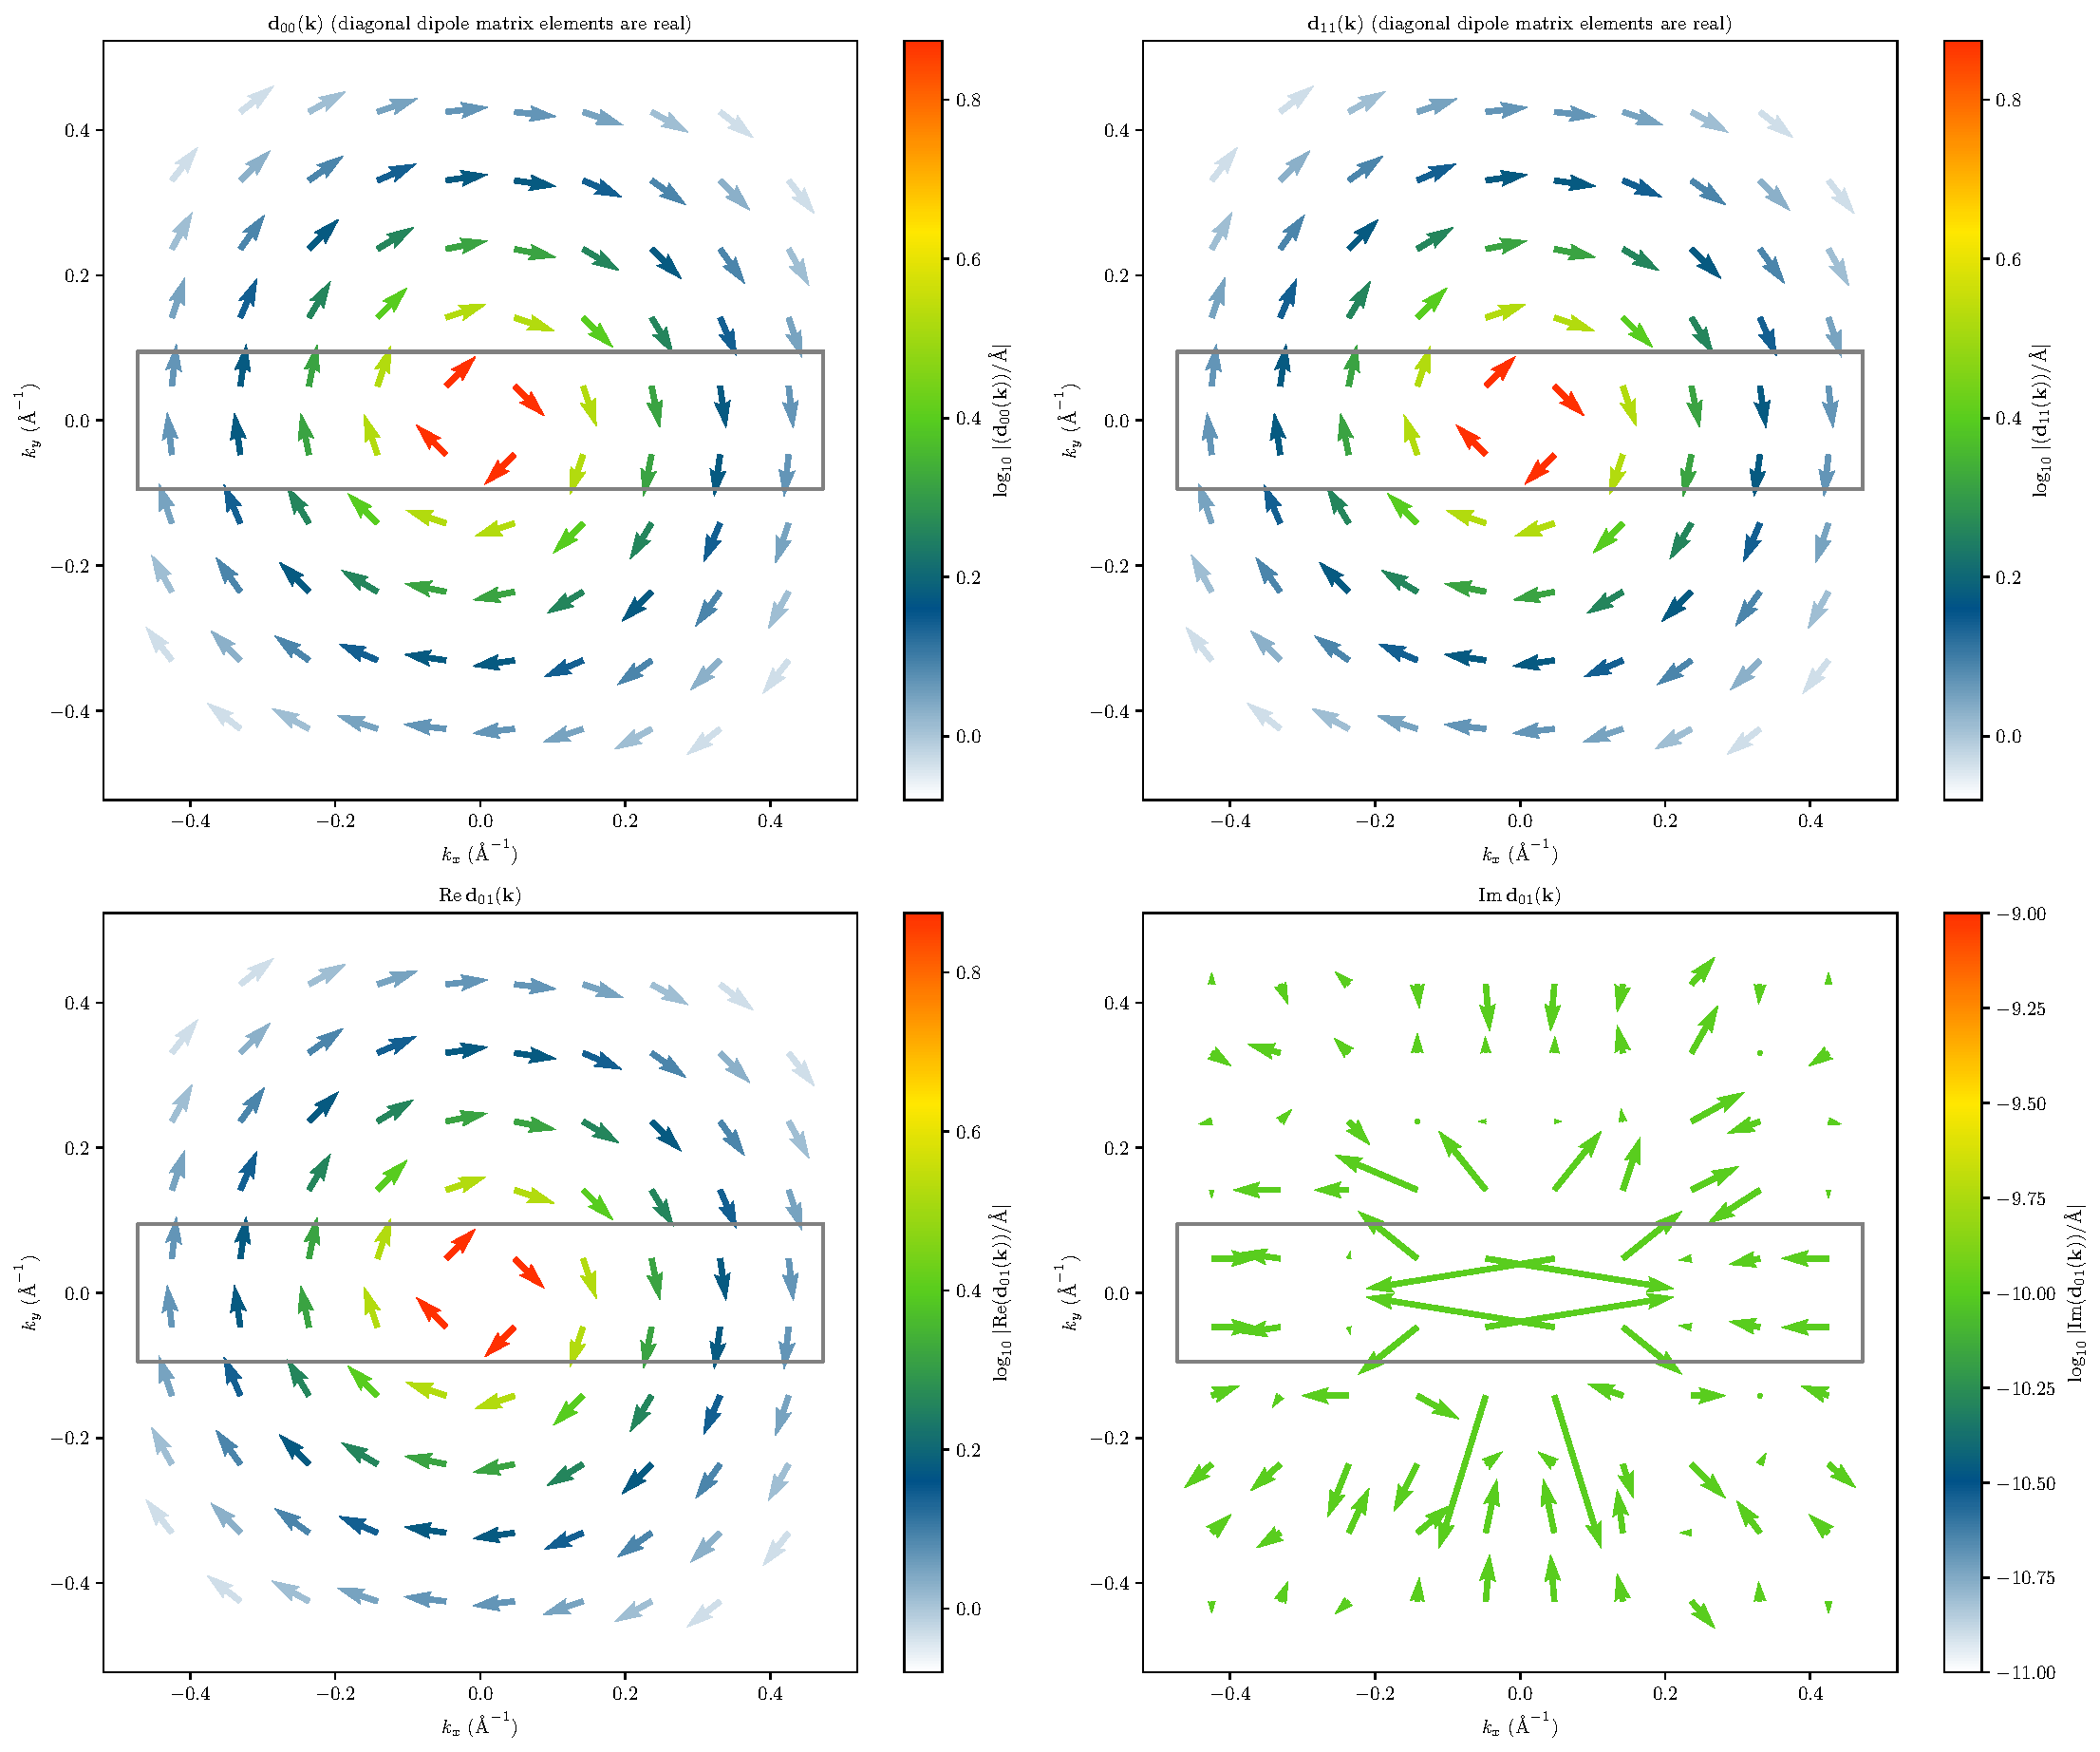
\includegraphics[width=\textwidth]{dipoles.pdf}
    \caption{Real and imaginary part of dipole matrix elements.}
    \label{fig:dipoles}
\end{figure}

The $n$-band Hamiltonian $h(\bk)$ is an $n\timest n$ matrix that is given as an input. 
%
Diagonalizing $h(\bk)$ yields the band structure and the eigenvectors~$\ketunk$,
\begin{align}
    h(\bk)\,\ketunk = \epsilon_n(\bk)\,\ketunk\,.
    \label{e3}
\end{align}
Dipoles are computed from
\begin{align}
\mathbf{d}_{nn'}(\bk) &=  iq\, \braunk \,\partial_{\bk}\,\ketunkprime\,,
\end{align}
where $q\eqt {-}\sd{e}$ is the electron charge.
%
The band structure and the dipoles are sketched in Fig.~\ref{fig:bandstructuredipole} and~\ref{fig:dipoles}. 
%{\color{red}How is the complex phase of $\ketunk$ made continuous?}

\section{Time evolution of the density matrix}
In case you choose the length gauge (\texttt{gauge = 'length'}, that is also the default) and $1/T_1\eqt 0$, we solve semiconductor Bloch equations in the length gauge, Eq.~(50) in Ref.~[\ref{Wilhelm2021}]:
\begin{align}
    \left[
    \frac{\partial}{\partial t}
    {+}q\bE(t)\frac{\partial}{\partial \bk}
    \right]\rhonnprime = 
    \left[i\sd(\epsilon_{n'}(\bk){-}\epsilon_{n}(\bk))
   \sd {-}\sd\frac{1{-}\sd\delta_{nn'}}{T_2}\right]\rhonnprime
    -i\sd \bE(t){\sum_{\un}}
    \big(\rho_{n\un}(\bk;t) \mathbf{d}_{\un n'}(\bk)
  \sd  {-} \sd \mathbf{d}_{n\un}(\bk)\rho_{\un n'}(\bk;t)
    \big)\label{e5}
\end{align}
with a dephasing time $T_2\eqt 10$\,fs. 
%
The time evolution of the density matrix is visualized in Figs.~\ref{fig:dm00}\,--\,\ref{fig:Imdm01}.
\\\\
\foreach \bandindex in {0,...,1}{
\begin{figure}
    \centering
    \includegraphics[width=\textwidth]{dm_\bandindex\bandindex.pdf}
    \caption{Time evolution of the \bandindex-\bandindex{} diagonal entry of the density matrix.}
    \label{fig:dm\bandindex\bandindex}
\end{figure}
}

\foreach \bandindex in {0,...,1}{
\foreach \jbandindex in {0,...,1}{
\ifnum \bandindex<\jbandindex
{
\begin{figure}
    \centering
    \includegraphics[width=\textwidth]{Re_dm_\bandindex\jbandindex.pdf}
    \caption{Time evolution of the real part of the \bandindex-\jbandindex{} offdiagonal entry of the density matrix.}    \label{fig:Redm\bandindex\jbandindex}
\end{figure}
\begin{figure}
    \centering
    \includegraphics[width=\textwidth]{Im_dm_\bandindex\jbandindex.pdf}
    \caption{Time evolution of the imaginary part of the \bandindex-\jbandindex{} offdiagonal entry of the density matrix.}       \label{fig:Imdm\bandindex\jbandindex}
\end{figure}
}
\fi
}
}

\section{Time-dependent current}
\begin{figure}
\centering
\setlength\figureheight{7.5cm} 
\setlength\figurewidth{7.5cm}
% This file was created with tikzplotlib v0.10.1.
\begin{tikzpicture}

\definecolor{darkgray176}{RGB}{176,176,176}
\definecolor{steelblue31119180}{RGB}{31,119,180}

\begin{axis}[
height=\figureheight,
tick align=outside,
tick pos=left,
width=\figurewidth,
x grid style={darkgray176},
xlabel={\(\displaystyle t \; (\si{\fs})\)},
xmajorgrids,
xmin=-92.0000000000078, xmax=92.4999999999927,
xtick style={color=black},
y grid style={darkgray176},
ylabel={Current \(\displaystyle j_{\parallel}(t)\) parallel to \(\displaystyle \bE\) in atomic units},
ymajorgrids,
ymin=-0.000255271091689042, ymax=0.00021728367372135,
ytick style={color=black}
]
\addplot [thick, steelblue31119180]
table {%
-92.0000000000078 -3.87846276457791e-08
-91.5000000000078 -4.18720129152121e-08
-91.0000000000078 -4.4895212877762e-08
-90.5000000000078 -4.78038619619107e-08
-90.0000000000078 -5.0541661773705e-08
-89.5000000000078 -5.30463192839502e-08
-89.0000000000078 -5.52495283542132e-08
-88.5000000000078 -5.70770300858007e-08
-88.0000000000078 -5.84488491567906e-08
-87.5000000000078 -5.92795437795268e-08
-87.0000000000078 -5.94785564587237e-08
-86.5000000000078 -5.8950775987837e-08
-86.0000000000078 -5.75971862549808e-08
-85.5000000000078 -5.53156251170419e-08
-85.0000000000078 -5.20017401338317e-08
-84.5000000000077 -4.7550092823509e-08
-84.0000000000077 -4.18553729771045e-08
-83.5000000000077 -3.48138079680434e-08
-83.0000000000077 -2.6324754134954e-08
-82.5000000000077 -1.62923944244034e-08
-82.0000000000077 -4.62760160803137e-09
-81.5000000000077 8.75000993669914e-09
-81.0000000000077 2.39099388672796e-08
-80.5000000000077 4.09085435090209e-08
-80.0000000000077 5.97866315847595e-08
-79.5000000000077 8.05669863843459e-08
-79.0000000000077 1.03251866145668e-07
-78.5000000000077 1.27820432329141e-07
-78.0000000000077 1.54226157806152e-07
-77.5000000000077 1.82394324334947e-07
-77.0000000000077 2.12219558107908e-07
-76.5000000000077 2.4356344529011e-07
-76.0000000000077 2.76252350822695e-07
-75.5000000000077 3.10075431345658e-07
-75.0000000000077 3.44782847048076e-07
-74.5000000000077 3.80084305636955e-07
-74.0000000000077 4.15647974293246e-07
-73.5000000000077 4.51099710961846e-07
-73.0000000000077 4.86022941764912e-07
-72.5000000000077 5.19958745430177e-07
-72.0000000000077 5.52406526311002e-07
-71.5000000000077 5.8282586725543e-07
-71.0000000000077 6.10638524593772e-07
-70.5000000000077 6.35231377173776e-07
-70.0000000000077 6.55960181545422e-07
-69.5000000000077 6.72154229760936e-07
-69.0000000000077 6.83121972575149e-07
-68.5000000000077 6.88157450625167e-07
-68.0000000000077 6.8654750646935e-07
-67.5000000000077 6.77579830948479e-07
-67.0000000000077 6.60551418338702e-07
-66.5000000000077 6.3477724181564e-07
-66.0000000000077 5.99599159881664e-07
-65.5000000000077 5.5439469878961e-07
-65.0000000000077 4.98585567276268e-07
-64.5000000000077 4.31646283266912e-07
-64.0000000000077 3.53113069813029e-07
-63.5000000000077 2.62593278188234e-07
-63.0000000000077 1.59776057007653e-07
-62.5000000000077 4.44448968741383e-08
-62.0000000000077 -8.3508009799581e-08
-61.5000000000077 -2.24065266762445e-07
-61.0000000000077 -3.77065813773984e-07
-60.5000000000077 -5.421858810907e-07
-60.0000000000077 -7.18920616707147e-07
-59.5000000000077 -9.06568180019774e-07
-59.0000000000077 -1.10421945656052e-06
-58.5000000000077 -1.31075661068268e-06
-58.0000000000077 -1.52486369990005e-06
-57.5000000000077 -1.74505363310663e-06
-57.0000000000077 -1.96971424814863e-06
-56.5000000000077 -2.1971733290668e-06
-56.0000000000077 -2.42577806023281e-06
-55.5000000000077 -2.65397560221111e-06
-55.0000000000076 -2.88037199604503e-06
-54.5000000000076 -3.10374176226989e-06
-54.0000000000076 -3.32297118676304e-06
-53.5000000000076 -3.5369572156667e-06
-53.0000000000076 -3.74455391851668e-06
-52.5000000000076 -3.94472730822768e-06
-52.0000000000076 -4.13706453593825e-06
-51.5000000000076 -4.3225902756113e-06
-51.0000000000076 -4.50447058898066e-06
-50.5000000000076 -4.68785808191387e-06
-50.0000000000076 -4.87828196416477e-06
-49.5000000000076 -5.07889599841618e-06
-49.0000000000076 -5.28817831982663e-06
-48.5000000000076 -5.50008402095936e-06
-48.0000000000076 -5.70704545394888e-06
-47.5000000000076 -5.90341398713181e-06
-47.0000000000076 -6.08590140201102e-06
-46.5000000000076 -6.25018222995221e-06
-46.0000000000076 -6.38686723046644e-06
-45.5000000000076 -6.48116900643502e-06
-45.0000000000076 -6.51713790507648e-06
-44.5000000000076 -6.48279540431496e-06
-44.0000000000076 -6.37175651478298e-06
-43.5000000000076 -6.18050756222597e-06
-43.0000000000076 -5.90416966619944e-06
-42.5000000000076 -5.53410727568693e-06
-42.0000000000076 -5.0588593164862e-06
-41.5000000000076 -4.46784961429754e-06
-41.0000000000076 -3.75622091128343e-06
-40.5000000000076 -2.92869415604049e-06
-40.0000000000076 -2.00039989907276e-06
-39.5000000000076 -9.93532190787292e-07
-39.0000000000076 6.93830749709272e-08
-38.5000000000076 1.17269251175589e-06
-38.0000000000076 2.31164514910459e-06
-37.5000000000076 3.49146043117822e-06
-37.0000000000076 4.72358736182493e-06
-36.5000000000076 6.02400033751823e-06
-36.0000000000076 7.41384493933503e-06
-35.5000000000076 8.91296388056398e-06
-35.0000000000076 1.0527957201516e-05
-34.5000000000076 1.22766705209323e-05
-34.0000000000076 1.42447481626885e-05
-33.5000000000076 1.65419526938193e-05
-33.0000000000076 1.9233589718662e-05
-32.5000000000076 2.24417281890751e-05
-32.0000000000076 2.62191412629949e-05
-31.5000000000076 3.04585226847193e-05
-31.0000000000076 3.50480835354937e-05
-30.5000000000076 3.96615282925204e-05
-30.0000000000076 4.4097700040904e-05
-29.5000000000076 4.81919922028961e-05
-29.0000000000076 5.20994354430136e-05
-28.5000000000076 5.60681703943831e-05
-28.0000000000076 6.03698940317993e-05
-27.5000000000076 6.49103425871205e-05
-27.0000000000076 6.93907049622452e-05
-26.5000000000075 7.34737429230567e-05
-26.0000000000075 7.72431766421116e-05
-25.5000000000075 8.09100986700615e-05
-25.0000000000075 8.4430964734719e-05
-24.5000000000075 8.74148302180632e-05
-24.0000000000075 8.97237389210937e-05
-23.5000000000075 9.17439307747654e-05
-23.0000000000075 9.33803315165664e-05
-22.5000000000075 9.42072015403103e-05
-22.0000000000075 9.44017823452787e-05
-21.5000000000076 9.4174897027335e-05
-21.0000000000076 9.32095092951245e-05
-20.5000000000076 9.16183289084939e-05
-20.0000000000076 8.95087307265969e-05
-19.5000000000076 8.6668598466481e-05
-19.0000000000076 8.35282543003404e-05
-18.5000000000076 7.99774668650973e-05
-18.0000000000076 7.56160612734393e-05
-17.5000000000076 7.12675290242971e-05
-17.0000000000076 6.68551220733768e-05
-16.5000000000076 6.12749527623792e-05
-16.0000000000076 5.51030982870394e-05
-15.5000000000076 4.89955264389107e-05
-15.0000000000076 4.17780600897613e-05
-14.5000000000076 3.19499467236461e-05
-14.0000000000076 1.95829302176746e-05
-13.5000000000076 5.49209862407509e-06
-13.0000000000076 -9.56166989633632e-06
-12.5000000000076 -2.48029002966641e-05
-12.0000000000076 -3.95395170128008e-05
-11.5000000000076 -5.38177767840425e-05
-11.0000000000076 -6.87086828478617e-05
-10.5000000000076 -8.50132208928781e-05
-10.0000000000076 -0.000101771979500635
-9.50000000000757 -0.000117682348769945
-9.00000000000757 -0.000133301336328592
-8.50000000000757 -0.000148527318118171
-8.00000000000757 -0.000161054524828362
-7.50000000000757 -0.000171731023089538
-7.00000000000757 -0.000182846388523717
-6.50000000000757 -0.000191862781329469
-6.00000000000757 -0.000200301444700357
-5.50000000000756 -0.000209445668824446
-5.00000000000756 -0.000216612278081924
-4.50000000000756 -0.000223887074067084
-4.00000000000756 -0.000228780671418532
-3.50000000000756 -0.000232684629844337
-3.00000000000756 -0.000233791329624934
-2.50000000000756 -0.000233772886340404
-2.00000000000756 -0.000233099294757625
-1.50000000000756 -0.000232287989176758
-1.00000000000756 -0.000231673761928027
-0.500000000007563 -0.000231604453370751
-7.5634022520587e-12 -0.000231815275623148
0.499999999992437 -0.000232233431464374
0.999999999992437 -0.000232411281265277
1.49999999999244 -0.000232666129090968
1.99999999999244 -0.000232557639590293
2.49999999999244 -0.000230919651112991
2.99999999999244 -0.00022847210616156
3.49999999999244 -0.00022276225218962
3.99999999999244 -0.000214818272243885
4.49999999999244 -0.000203876812583278
4.99999999999244 -0.000191353595355133
5.49999999999244 -0.000176903652215112
5.99999999999244 -0.000161359475715142
6.49999999999244 -0.000144233494617745
6.99999999999244 -0.000126152776320974
7.49999999999244 -0.000107444220635058
7.99999999999244 -8.88069132903596e-05
8.49999999999244 -6.95976300716354e-05
8.99999999999244 -4.94767030290212e-05
9.49999999999244 -2.91222937381546e-05
9.99999999999244 -9.50887441568562e-06
10.4999999999924 8.98657579971313e-06
10.9999999999924 2.68507889515123e-05
11.4999999999924 4.36365780769702e-05
11.9999999999924 5.96542649276977e-05
12.4999999999924 7.69109216236452e-05
12.9999999999924 9.26598875613843e-05
13.4999999999924 0.000106203496733052
13.9999999999924 0.000121056917267438
14.4999999999924 0.000133497183537632
14.9999999999924 0.000145353264428055
15.4999999999924 0.000155883498162269
15.9999999999924 0.000165111233684037
16.4999999999924 0.000173728218860617
16.9999999999924 0.000180824960030341
17.4999999999924 0.000186834359439921
17.9999999999924 0.000190982317514522
18.4999999999924 0.00019396473296626
18.9999999999924 0.000195344845981941
19.4999999999924 0.000195803911657241
19.9999999999924 0.000195364401553974
20.4999999999924 0.000194364324164953
20.9999999999924 0.000192670080482968
21.4999999999924 0.000190093846710105
21.9999999999924 0.000186939845330636
22.4999999999924 0.000182840631829171
22.9999999999924 0.000178255089050993
23.4999999999924 0.000172882145913132
23.9999999999924 0.000166936444202804
24.4999999999924 0.000160459658866686
24.9999999999924 0.000153024193890091
25.4999999999924 0.000144828925121187
25.9999999999924 0.000135508324221911
26.4999999999924 0.000126066380015777
26.9999999999924 0.000116138695936051
27.4999999999924 0.000105837329883176
27.9999999999924 9.60582250307558e-05
28.4999999999924 8.69157796653092e-05
28.9999999999924 7.76796160516385e-05
29.4999999999924 6.78650065461589e-05
29.9999999999924 5.78940099547115e-05
30.4999999999924 4.8144468327577e-05
30.9999999999924 3.91547502795126e-05
31.4999999999924 3.06805563461752e-05
31.9999999999924 2.22288723910197e-05
32.4999999999924 1.41315167893819e-05
32.9999999999924 7.00543878954873e-06
33.4999999999924 4.24188019707244e-07
33.9999999999925 -6.12384254479232e-06
34.4999999999925 -1.21198156634984e-05
34.9999999999925 -1.70489210646083e-05
35.4999999999925 -2.1468543874962e-05
35.9999999999925 -2.57310798278845e-05
36.4999999999925 -2.91360027772413e-05
36.9999999999925 -3.18010010930727e-05
37.4999999999925 -3.42921535029131e-05
37.9999999999925 -3.60353111170529e-05
38.4999999999925 -3.71659893678208e-05
38.9999999999925 -3.81450505507335e-05
39.4999999999925 -3.84336591729368e-05
39.9999999999925 -3.83774738213472e-05
40.4999999999925 -3.81488948571285e-05
40.9999999999925 -3.72063093698529e-05
41.4999999999925 -3.61187009722759e-05
41.9999999999925 -3.49475397294779e-05
42.4999999999925 -3.32510658023394e-05
42.9999999999925 -3.15273268338501e-05
43.4999999999925 -2.97732773897714e-05
43.9999999999925 -2.76629203185022e-05
44.4999999999925 -2.54486260148142e-05
44.9999999999925 -2.31340644829453e-05
45.4999999999925 -2.066071045684e-05
45.9999999999925 -1.82257818107117e-05
46.4999999999925 -1.57288383930008e-05
46.9999999999925 -1.30350840679324e-05
47.4999999999925 -1.03310693476531e-05
47.9999999999925 -7.6762954177674e-06
48.4999999999925 -4.92128732287737e-06
48.9999999999925 -2.11428358957221e-06
49.4999999999925 5.72703076262095e-07
49.9999999999925 3.14441756307686e-06
50.4999999999925 5.65558593030394e-06
50.9999999999925 8.05021872010279e-06
51.4999999999925 1.03018675919079e-05
51.9999999999925 1.24432940895146e-05
52.4999999999925 1.44355139651659e-05
52.9999999999925 1.62205675485293e-05
53.4999999999925 1.78258670854625e-05
53.9999999999925 1.92979639222063e-05
54.4999999999925 2.06357102223896e-05
54.9999999999925 2.18163141643371e-05
55.4999999999925 2.28331980941176e-05
55.9999999999925 2.37266017030414e-05
56.4999999999925 2.45388749089198e-05
56.9999999999925 2.52354228636906e-05
57.4999999999925 2.57813663809589e-05
57.9999999999925 2.62276086108098e-05
58.4999999999925 2.65915038277095e-05
58.9999999999925 2.68056866106192e-05
59.4999999999925 2.68729831993543e-05
59.9999999999925 2.68766741180759e-05
60.4999999999925 2.6826095421674e-05
60.9999999999925 2.66797442792375e-05
61.4999999999925 2.64717317729508e-05
61.9999999999925 2.62630816615019e-05
62.4999999999926 2.60321224517001e-05
62.9999999999926 2.57218800219287e-05
63.4999999999926 2.53390653422044e-05
63.9999999999926 2.4925232773414e-05
64.4999999999926 2.44838540115954e-05
64.9999999999926 2.40099751980122e-05
65.4999999999926 2.35383388598396e-05
65.9999999999926 2.30984235971282e-05
66.4999999999926 2.26752164670583e-05
66.9999999999926 2.2251562548951e-05
67.4999999999926 2.18353891664031e-05
67.9999999999926 2.14318486495866e-05
68.4999999999926 2.10312318310523e-05
68.9999999999926 2.06269839762515e-05
69.4999999999926 2.02273456972188e-05
69.9999999999926 1.98481812349883e-05
70.4999999999926 1.94936670441244e-05
70.9999999999926 1.91544738498624e-05
71.4999999999926 1.88327967892441e-05
71.9999999999926 1.85437585327578e-05
72.4999999999926 1.82855184075665e-05
72.9999999999926 1.80430017657283e-05
73.4999999999926 1.78196703721306e-05
73.9999999999926 1.76280666394495e-05
74.4999999999926 1.74603728005208e-05
74.9999999999926 1.7303475957507e-05
75.4999999999926 1.71642583371584e-05
75.9999999999926 1.70505734856043e-05
76.4999999999926 1.69515071946668e-05
76.9999999999926 1.68595780546132e-05
77.4999999999926 1.67850166669184e-05
77.9999999999926 1.67322080196408e-05
78.4999999999926 1.66913725507814e-05
78.9999999999926 1.66609599048946e-05
79.4999999999926 1.66479012815295e-05
79.9999999999926 1.664664256389e-05
80.4999999999926 1.66462458927454e-05
80.9999999999926 1.6649142995647e-05
81.4999999999926 1.66599626063864e-05
81.9999999999926 1.66721912922674e-05
82.4999999999926 1.66821818861523e-05
82.9999999999926 1.66967697423707e-05
83.4999999999926 1.67186498560343e-05
83.9999999999926 1.67431085573611e-05
84.4999999999926 1.67696658005282e-05
84.9999999999926 1.68006561627575e-05
85.4999999999926 1.68325838060416e-05
85.9999999999926 1.68605077283444e-05
86.4999999999926 1.68849913297229e-05
86.9999999999926 1.6908452876393e-05
87.4999999999926 1.6930635642293e-05
87.9999999999926 1.69506222377498e-05
88.4999999999926 1.69693839975145e-05
88.9999999999926 1.69887800660701e-05
89.4999999999926 1.70089429667883e-05
89.9999999999926 1.70278751426621e-05
90.4999999999927 1.70446225192913e-05
90.9999999999927 1.70605392253954e-05
91.4999999999927 1.70756478577578e-05
91.9999999999927 1.70877017075838e-05
92.4999999999927 1.70965076512437e-05
};
\end{axis}

\end{tikzpicture}
\hfill% This file was created with tikzplotlib v0.10.1.
\begin{tikzpicture}

\definecolor{darkgray176}{RGB}{176,176,176}
\definecolor{steelblue31119180}{RGB}{31,119,180}

\begin{axis}[
height=\figureheight,
tick align=outside,
tick pos=left,
width=\figurewidth,
x grid style={darkgray176},
xlabel={\(\displaystyle t \; (\si{\fs})\)},
xmajorgrids,
xmin=-92.0000000000078, xmax=92.4999999999927,
xtick style={color=black},
y grid style={darkgray176},
ylabel={Current \(\displaystyle j_{\bot}(t)\) orthogonal to \(\displaystyle \bE\) in atomic units},
ymajorgrids,
ymin=-1.25583812290442e-14, ymax=1.37769335846789e-14,
ytick style={color=black}
]
\addplot [thick, steelblue31119180]
table {%
-92.0000000000078 -5.68130214758217e-21
-91.5000000000078 -5.89327270036023e-21
-91.0000000000078 -6.38553914883065e-21
-90.5000000000078 -5.57729614985033e-21
-90.0000000000078 -6.69762150881175e-21
-89.5000000000078 -6.83189062357314e-21
-89.0000000000078 -7.08982978906713e-21
-88.5000000000078 -1.03232738080828e-20
-88.0000000000078 -9.39300211140267e-21
-87.5000000000078 -1.10178343358961e-20
-87.0000000000078 -9.33567276102836e-21
-86.5000000000078 -8.75697244729488e-21
-86.0000000000078 -8.6841950683766e-21
-85.5000000000078 -1.13333603189068e-20
-85.0000000000078 -1.16524479307207e-20
-84.5000000000077 -1.12399855685965e-20
-84.0000000000077 -1.00154718393441e-20
-83.5000000000077 -9.51512735928087e-21
-83.0000000000077 -1.07696789218133e-20
-82.5000000000077 -1.19167808635843e-20
-82.0000000000077 -1.07502830637525e-20
-81.5000000000077 -1.19902448215489e-20
-81.0000000000077 -1.44821834704538e-20
-80.5000000000077 -1.75668114811625e-20
-80.0000000000077 -2.53519312882797e-20
-79.5000000000077 -1.31162344576432e-21
-79.0000000000077 -9.72367574462454e-23
-78.5000000000077 3.36664035401705e-21
-78.0000000000077 2.44078850994812e-21
-77.5000000000077 -4.41298682072898e-22
-77.0000000000077 -3.11629646922385e-21
-76.5000000000077 -4.96225005784811e-21
-76.0000000000077 -1.01512428457695e-20
-75.5000000000077 -1.34416729256362e-20
-75.0000000000077 -1.76419918867432e-20
-74.5000000000077 -1.75008998927082e-20
-74.0000000000077 -9.51117952976408e-21
-73.5000000000077 -2.07525382564534e-20
-73.0000000000077 6.90286573249463e-21
-72.5000000000077 2.51466441534064e-20
-72.0000000000077 6.00729202437189e-20
-71.5000000000077 4.97495177020649e-20
-71.0000000000077 5.10567642064084e-20
-70.5000000000077 8.76431884309135e-20
-70.0000000000077 7.22940272696195e-20
-69.5000000000077 4.05246416346492e-20
-69.0000000000077 8.70087893920409e-20
-68.5000000000077 3.77288917577128e-20
-68.0000000000077 -9.00791708875368e-21
-67.5000000000077 -2.27394980167319e-20
-67.0000000000077 -5.57282480381066e-20
-66.5000000000077 -4.6149097182749e-20
-66.0000000000077 -3.81188686560674e-20
-65.5000000000077 -1.72611464897057e-19
-65.0000000000077 -1.00339408156922e-19
-64.5000000000077 -6.11000424971317e-20
-64.0000000000077 -7.05253996460959e-20
-63.5000000000077 -2.14146750888005e-19
-63.0000000000077 -6.90753447001014e-20
-62.5000000000077 -3.54824051178956e-20
-62.0000000000077 -3.34567222994003e-19
-61.5000000000077 -7.4721770777686e-20
-61.0000000000077 -1.07655594475349e-21
-60.5000000000077 -2.90977692496229e-19
-60.0000000000077 -6.4439562978816e-20
-59.5000000000077 -1.71809540570863e-20
-59.0000000000077 3.85802497752475e-20
-58.5000000000077 6.98443132320682e-20
-58.0000000000077 -2.64744880291419e-21
-57.5000000000077 -6.63839548382177e-20
-57.0000000000077 -1.1480700182264e-19
-56.5000000000077 -2.6073525866045e-19
-56.0000000000077 -4.2552521506093e-19
-55.5000000000077 -5.3074208076347e-19
-55.0000000000076 -6.82866026915983e-19
-54.5000000000076 -9.01846294290637e-19
-54.0000000000076 -1.02593584482059e-18
-53.5000000000076 -1.14343423650511e-18
-53.0000000000076 -1.28422138944349e-18
-52.5000000000076 -1.44012426666738e-18
-52.0000000000076 -1.29292171911946e-18
-51.5000000000076 -1.30909202882024e-18
-51.0000000000076 -1.3632274134707e-18
-50.5000000000076 -1.32561386699279e-18
-50.0000000000076 -9.74085395236544e-19
-49.5000000000076 -8.96749131450171e-19
-49.0000000000076 3.10751169032517e-19
-48.5000000000076 1.87610745376306e-18
-48.0000000000076 2.37879316837448e-18
-47.5000000000076 3.99687872386846e-19
-47.0000000000076 1.08270769300922e-19
-46.5000000000076 -1.66062050057648e-18
-46.0000000000076 -1.94043716409445e-18
-45.5000000000076 -1.70210086024372e-18
-45.0000000000076 -1.95098301824714e-18
-44.5000000000076 -2.57248535631217e-18
-44.0000000000076 -3.46817990234708e-18
-43.5000000000076 -3.67980004234433e-18
-43.0000000000076 -2.68848975199173e-18
-42.5000000000076 1.78646769346522e-18
-42.0000000000076 6.58483133293791e-18
-41.5000000000076 8.86625111463592e-18
-41.0000000000076 4.73719768538711e-18
-40.5000000000076 -1.1519588019452e-17
-40.0000000000076 -3.37727463955091e-17
-39.5000000000076 -4.45485001687249e-17
-39.0000000000076 -3.3258108712858e-17
-38.5000000000076 -6.34297974436962e-18
-38.0000000000076 3.01520031364198e-17
-37.5000000000076 6.33306664146609e-17
-37.0000000000076 7.30644897975912e-17
-36.5000000000076 5.7677385531877e-17
-36.0000000000076 2.52467748415332e-17
-35.5000000000076 -1.25516756125283e-17
-35.0000000000076 -4.17222112558048e-17
-34.5000000000076 -6.30684261747307e-17
-34.0000000000076 -7.38603502576474e-17
-33.5000000000076 -5.34070176569822e-17
-33.0000000000076 -3.78399308137288e-17
-32.5000000000076 -4.05762284378794e-17
-32.0000000000076 7.70409798700978e-17
-31.5000000000076 -6.6406540542528e-17
-31.0000000000076 1.17199592483531e-17
-30.5000000000076 -8.21929811521573e-17
-30.0000000000076 7.20831629158365e-16
-29.5000000000076 4.83391019853668e-16
-29.0000000000076 7.4900312088491e-16
-28.5000000000076 3.5888807184093e-16
-28.0000000000076 -3.88070559452246e-16
-27.5000000000076 6.15006091906979e-17
-27.0000000000076 1.25558095873562e-15
-26.5000000000075 1.43551010394711e-15
-26.0000000000075 7.74555022439928e-16
-25.5000000000075 -6.06068832041048e-16
-25.0000000000075 -1.39662543051532e-15
-24.5000000000075 -1.13259098926532e-15
-24.0000000000075 -1.78087136019486e-16
-23.5000000000075 -6.02966944806271e-16
-23.0000000000075 -9.32998747457675e-16
-22.5000000000075 1.48427694577691e-15
-22.0000000000075 1.40169868941971e-15
-21.5000000000076 -8.76880742226508e-17
-21.0000000000076 1.38029201160364e-15
-20.5000000000076 -9.61390999064483e-16
-20.0000000000076 -2.62492215538711e-15
-19.5000000000076 1.30091969490885e-15
-19.0000000000076 1.76433546088344e-16
-18.5000000000076 -1.01881669021058e-15
-18.0000000000076 2.61645453755944e-15
-17.5000000000076 1.00555984848371e-15
-17.0000000000076 -2.56748521532991e-15
-16.5000000000076 -4.28234796521227e-16
-16.0000000000076 1.5580023091014e-15
-15.5000000000076 -5.22601911707246e-16
-15.0000000000076 -2.18198221983537e-15
-14.5000000000076 -6.9220174430465e-16
-14.0000000000076 6.55535918586587e-16
-13.5000000000076 8.42447825361041e-16
-13.0000000000076 7.03445030945301e-16
-12.5000000000076 3.77772181343675e-16
-12.0000000000076 3.24598578591939e-16
-11.5000000000076 8.82083363608501e-17
-11.0000000000076 2.05748208405041e-16
-10.5000000000076 7.27618940891034e-16
-10.0000000000076 6.88661149537121e-16
-9.50000000000757 -4.51556601451423e-16
-9.00000000000757 -4.29241574064337e-16
-8.50000000000757 -1.12441303089838e-16
-8.00000000000757 -2.30200810123182e-15
-7.50000000000757 4.04547964425959e-15
-7.00000000000757 2.70439852450953e-15
-6.50000000000757 -1.60203617158748e-15
-6.00000000000757 -1.9317080090838e-15
-5.50000000000756 2.15032497178289e-15
-5.00000000000756 -2.19836344661921e-15
-4.50000000000756 1.30115029758633e-15
-4.00000000000756 1.60583267908244e-15
-3.50000000000756 1.13387336513029e-15
-3.00000000000756 -9.28563864257998e-16
-2.50000000000756 -2.23087279968723e-15
-2.00000000000756 2.49492973875942e-15
-1.50000000000756 -5.14747359534325e-16
-1.00000000000756 1.23042558129674e-15
-0.500000000007563 -4.901066197781e-16
-7.5634022520587e-12 -3.29115578842618e-15
0.499999999992437 7.03646948899478e-15
0.999999999992437 -5.38920425811726e-15
1.49999999999244 -2.74614042135976e-17
1.99999999999244 5.50407813823165e-15
2.49999999999244 -9.65052800849073e-15
2.99999999999244 1.25798738204187e-14
3.49999999999244 -1.1361321464784e-14
3.99999999999244 8.59106900248958e-15
4.49999999999244 -6.40836404011628e-15
4.99999999999244 5.76431325975891e-15
5.49999999999244 -4.34534749180654e-15
5.99999999999244 3.98207515686586e-15
6.49999999999244 -3.27640846597906e-15
6.99999999999244 4.15063446518687e-15
7.49999999999244 -3.66406281572075e-15
7.99999999999244 1.59548368087394e-15
8.49999999999244 2.8916563353002e-15
8.99999999999244 -1.25487790179211e-15
9.49999999999244 1.84918037282653e-15
9.99999999999244 2.80117571889791e-15
10.4999999999924 -4.19471894777288e-16
10.9999999999924 -2.4921793799964e-15
11.4999999999924 -2.09225809270431e-15
11.9999999999924 2.5470909395125e-16
12.4999999999924 1.80342542694274e-15
12.9999999999924 4.66791564194561e-15
13.4999999999924 2.90946898602103e-15
13.9999999999924 -1.06901776820515e-15
14.4999999999924 -6.06890002551071e-16
14.9999999999924 -2.12660664273656e-17
15.4999999999924 1.281700930301e-15
15.9999999999924 -4.95391920656649e-15
16.4999999999924 4.59354909068864e-15
16.9999999999924 -4.73630902141051e-15
17.4999999999924 2.71526216040069e-16
17.9999999999924 -1.76006649912244e-15
18.4999999999924 1.09260673477388e-15
18.9999999999924 -1.84549072998698e-15
19.4999999999924 1.24879786534461e-16
19.9999999999924 1.00088873815101e-15
20.4999999999924 -2.00249178215664e-15
20.9999999999924 2.64578326101501e-15
21.4999999999924 -6.44191391746069e-16
21.9999999999924 7.2477577861147e-16
22.4999999999924 8.33524626633981e-16
22.9999999999924 -9.68137533494429e-16
23.4999999999924 -2.94957697853453e-16
23.9999999999924 -1.58577587059792e-15
24.4999999999924 -7.57119210240818e-16
24.9999999999924 -3.14019540151518e-15
25.4999999999924 -2.48944027014448e-16
25.9999999999924 -1.42857233802853e-15
26.4999999999924 -3.95579207608959e-16
26.9999999999924 2.30253961228112e-16
27.4999999999924 6.24893884760539e-16
27.9999999999924 1.00248045907113e-15
28.4999999999924 2.74822146991255e-16
28.9999999999924 8.09122926238549e-16
29.4999999999924 -8.27121183992469e-16
29.9999999999924 -3.98998876582204e-16
30.4999999999924 8.59135584972253e-17
30.9999999999924 -5.06510344384133e-16
31.4999999999924 9.90764718164434e-16
31.9999999999924 9.22056369188847e-16
32.4999999999924 -1.33935159966902e-15
32.9999999999924 -9.57372325575366e-16
33.4999999999924 7.88919881909775e-16
33.9999999999925 1.39992698592205e-16
34.4999999999925 -8.83922560572729e-16
34.9999999999925 5.17899866869035e-17
35.4999999999925 8.002419109281e-16
35.9999999999925 9.97328457789067e-17
36.4999999999925 -4.14049919628919e-16
36.9999999999925 1.49616142035004e-16
37.4999999999925 4.58781214602957e-16
37.9999999999925 -1.3370455728943e-16
38.4999999999925 -2.61098475453892e-16
38.9999999999925 3.34851961056125e-16
39.4999999999925 -9.78711509924856e-17
39.9999999999925 -3.75522399124435e-16
40.4999999999925 1.23844886713611e-16
40.9999999999925 -4.15860994315407e-16
41.4999999999925 -2.39719919915564e-16
41.9999999999925 2.43915763754447e-16
42.4999999999925 -3.48058182683064e-16
42.9999999999925 -7.19030397269086e-17
43.4999999999925 2.17390831389608e-16
43.9999999999925 -4.04353358263995e-16
44.4999999999925 -1.5939707023315e-17
44.9999999999925 3.94983015320861e-16
45.4999999999925 -9.28372632769363e-17
45.9999999999925 -2.33583638912587e-17
46.4999999999925 2.6631234574698e-16
46.9999999999925 6.27014304502172e-17
47.4999999999925 -1.64700931815008e-16
47.9999999999925 -6.13740589408657e-17
48.4999999999925 9.09361973016785e-17
48.9999999999925 2.34483551800283e-17
49.4999999999925 -1.55718676304693e-16
49.9999999999925 -1.46353957817106e-16
50.4999999999925 3.76557298945286e-17
50.9999999999925 -1.34930688598916e-17
51.4999999999925 -2.19168159342807e-16
51.9999999999925 -6.4096295426146e-17
52.4999999999925 1.86135731908817e-16
52.9999999999925 1.24637934945893e-17
53.4999999999925 -1.14452045948284e-16
53.9999999999925 8.96369480700675e-17
54.4999999999925 4.4438823285537e-17
54.9999999999925 -2.19241277264932e-16
55.4999999999925 -1.24210476324237e-16
55.9999999999925 5.44897253499914e-17
56.4999999999925 -5.29654978964564e-17
56.9999999999925 -7.90348493618992e-17
57.4999999999925 9.2314188910963e-17
57.9999999999925 5.99735695093888e-17
58.4999999999925 -1.42411214477888e-16
58.9999999999925 -1.56708580481158e-16
59.4999999999925 5.81006258118715e-18
59.9999999999925 4.8156588402831e-17
60.4999999999925 -7.23811184484971e-17
60.9999999999925 -6.40175530484726e-17
61.4999999999925 7.23080005263718e-17
61.9999999999925 7.78424647857021e-18
62.4999999999926 -1.27112695387057e-16
62.9999999999926 -3.40335805215522e-17
63.4999999999926 2.66205481091566e-17
63.9999999999926 -8.21732955577389e-17
64.4999999999926 -9.15436385008733e-17
64.9999999999926 1.11139241630453e-17
65.4999999999926 2.13616821716833e-17
65.9999999999926 -3.05182958039898e-17
66.4999999999926 -6.29939021387184e-17
66.9999999999926 -5.8634949088941e-17
67.4999999999926 -1.12770333739402e-17
67.9999999999926 -1.23175576503387e-18
68.4999999999926 -5.02263880445317e-17
68.9999999999926 -4.04173375686456e-17
69.4999999999926 3.25093530680172e-18
69.9999999999926 -2.27340493254196e-17
70.4999999999926 -3.95624203253344e-17
70.9999999999926 -5.43322405946446e-18
71.4999999999926 -2.60862248320871e-17
71.9999999999926 -6.14134301297024e-17
72.4999999999926 -3.23518683126704e-17
72.9999999999926 -1.68564932776553e-17
73.4999999999926 -3.65870833403896e-17
73.9999999999926 -2.28352895252854e-17
74.4999999999926 -1.1940719128616e-17
74.9999999999926 -3.22281302906122e-17
75.4999999999926 -3.03776844152873e-17
75.9999999999926 -2.70986268307451e-17
76.4999999999926 -4.64636272828529e-17
76.9999999999926 -3.32236589226259e-17
77.4999999999926 -1.13614002071617e-17
77.9999999999926 -3.74476250392489e-17
78.4999999999926 -4.47875395295192e-17
78.9999999999926 -4.0721058168243e-18
79.4999999999926 -9.98340859787725e-18
79.9999999999926 -4.88596453463435e-17
80.4999999999926 -3.28018247565184e-17
80.9999999999926 -1.43029904588179e-17
81.4999999999926 -3.45229081542369e-17
81.9999999999926 -3.70932843397186e-17
82.4999999999926 -1.78407729985728e-17
82.9999999999926 -2.37070801352409e-17
83.4999999999926 -3.51134759867874e-17
83.9999999999926 -2.67892817755996e-17
84.4999999999926 -2.01355508621975e-17
84.9999999999926 -2.64630633538098e-17
85.4999999999926 -3.3285527933655e-17
85.9999999999926 -3.33305235780398e-17
86.4999999999926 -2.5287552144257e-17
86.9999999999926 -2.17778918822427e-17
87.4999999999926 -3.00964616378823e-17
87.9999999999926 -3.21887591017755e-17
88.4999999999926 -2.36958312241447e-17
88.9999999999926 -2.57600064102974e-17
89.4999999999926 -3.17894227578604e-17
89.9999999999926 -2.68230285088882e-17
90.4999999999927 -2.54787836328924e-17
90.9999999999927 -3.19412830576591e-17
91.4999999999927 -2.91403041947054e-17
91.9999999999927 -2.35214731021536e-17
92.4999999999927 -2.66149236536085e-17
};
\end{axis}

\end{tikzpicture}

\\
\setlength\figureheight{6.5cm} 
\setlength\figurewidth{\textwidth}
% This file was created with tikzplotlib v0.10.1.
\begin{tikzpicture}

\definecolor{darkgray176}{RGB}{176,176,176}
\definecolor{steelblue31119180}{RGB}{31,119,180}

\begin{axis}[
height=\figureheight,
tick align=outside,
tick pos=left,
width=\figurewidth,
x grid style={darkgray176},
xlabel={\(\displaystyle t \; (\si{\fs})\)},
xmajorgrids,
xmin=-400, xmax=399.499999999985,
xtick style={color=black},
y grid style={darkgray176},
ylabel={Current \(\displaystyle j_{\parallel}(t)\) parallel to \(\displaystyle \bE\) in atomic units},
ymajorgrids,
ymin=-0.000255271091689042, ymax=0.00021728367372135,
ytick style={color=black}
]
\addplot [thick, steelblue31119180]
table {%
-400 0
-399.5 4.11613854924621e-63
-399 1.50732111720716e-62
-398.5 3.5204797123909e-62
-398 6.81468390025545e-62
-397.5 1.24437576631871e-61
-397 2.23414678633055e-61
-396.5 3.51744812746443e-61
-396 4.21524260561145e-61
-395.5 7.12658370139911e-61
-395 2.71471858002498e-60
-394.5 4.32859644323245e-60
-394 -1.43524954496594e-59
-393.5 -3.87136186680295e-59
-393 2.09329414311353e-58
-392.5 7.31250489859222e-58
-392 -2.30773456897828e-57
-391.5 -1.17290110342903e-56
-391 2.44423362935752e-56
-390.5 1.84911149074559e-55
-390 -2.15412193466199e-55
-389.5 -2.82480190696844e-54
-389 1.03189960792089e-54
-388.5 4.19121715242494e-53
-388 1.63418598446158e-53
-387.500000000001 -6.02774696345379e-52
-387.000000000001 -6.97071829207677e-52
-386.500000000001 8.3696106759498e-51
-386.000000000001 1.67062755643147e-50
-385.500000000001 -1.11376834700847e-49
-385.000000000001 -3.33914365355602e-49
-384.500000000001 1.40161863989024e-48
-384.000000000001 6.06386947272474e-48
-383.500000000001 -1.62481618510333e-47
-383.000000000001 -1.03325856505132e-46
-382.500000000001 1.63093125502023e-46
-382.000000000001 1.67648478047342e-45
-381.500000000001 -1.1409094256204e-45
-381.000000000001 -2.6080667422995e-44
-380.500000000001 -3.24143898361746e-45
-380.000000000001 3.89952571313052e-43
-379.500000000001 3.54572155195006e-43
-379.000000000001 -5.5978185776609e-42
-378.500000000001 -9.74475532547748e-42
-378.000000000001 7.67797784588764e-41
-377.500000000001 2.07517086204614e-40
-377.000000000001 -9.95779893689577e-40
-376.500000000001 -3.91969938123823e-39
-376.000000000001 1.19533338273818e-38
-375.500000000001 6.86852104327077e-38
-375.000000000001 -1.26458690792008e-37
-374.500000000001 -1.13874499819491e-36
-374.000000000001 1.01221668680945e-36
-373.500000000001 1.80311208796275e-35
-373.000000000001 -1.04190921755001e-36
-372.500000000001 -2.73755955729195e-34
-372.000000000001 -2.01165184462979e-34
-371.500000000001 3.98561886347404e-33
-371.000000000001 6.2071060623296e-33
-370.500000000001 -5.5440773098648e-32
-370.000000000001 -1.3801571168304e-31
-369.500000000001 7.30324783923788e-31
-369.000000000001 2.67086320086924e-30
-368.500000000001 -8.94471290922105e-30
-368.000000000001 -4.75770105927039e-29
-367.500000000001 9.77501606227314e-29
-367.000000000001 7.98719853072263e-28
-366.500000000001 -8.46694483385378e-28
-366.000000000001 -1.2779293831846e-26
-365.500000000001 2.67370729134696e-27
-365.000000000001 1.95841147166487e-25
-364.500000000001 1.15218175290752e-25
-364.000000000001 -2.87725775177096e-24
-363.500000000001 -4.03552602323634e-24
-363.000000000001 4.0410890855626e-23
-362.500000000001 9.3335912391416e-23
-362.000000000002 -5.38425011935439e-22
-361.500000000002 -1.84362411030421e-21
-361.000000000002 6.69652141380891e-21
-360.500000000002 3.32839102279956e-20
-360.000000000002 -7.50459607992789e-20
-359.500000000002 -5.64425164839589e-19
-359.000000000002 6.88636050165707e-19
-358.500000000002 1.01422491863442e-18
-358.000000000002 -1.09338756179526e-18
-357.500000000002 2.91970325485338e-19
-357.000000000002 -1.96944612682426e-18
-356.500000000002 -8.362476429002e-18
-356.000000000002 2.19963739133829e-18
-355.500000000002 4.92810337436053e-18
-355.000000000002 -3.81735043333578e-19
-354.500000000002 -8.29954715222588e-19
-354.000000000002 1.44415231521329e-18
-353.500000000002 -7.28495801339642e-19
-353.000000000002 9.23723093968106e-20
-352.500000000002 -1.71325858046129e-19
-352.000000000002 -4.51494671859366e-19
-351.500000000002 3.85139205074035e-19
-351.000000000002 -5.56068667163532e-19
-350.500000000002 8.53511070500303e-19
-350.000000000002 -1.68209184570975e-18
-349.500000000002 2.41257019364998e-18
-349.000000000002 -2.05564679021366e-18
-348.500000000002 1.87860362960704e-18
-348.000000000002 -1.26135755865659e-18
-347.500000000002 1.6415169286153e-18
-347.000000000002 -1.8525246691986e-18
-346.500000000002 1.87667141292416e-18
-346.000000000002 -1.6577210592454e-18
-345.500000000002 9.19656224502741e-19
-345.000000000002 -3.61200279711262e-19
-344.500000000002 -3.61887700845937e-19
-344.000000000002 1.80015896762589e-19
-343.500000000002 -5.93788248698936e-19
-343.000000000002 4.79372216764044e-19
-342.500000000002 -9.06312382722213e-19
-342.000000000002 1.54281379554637e-18
-341.500000000002 -1.970912667592e-18
-341.000000000002 2.42773660452343e-18
-340.500000000002 -2.03870661710706e-18
-340.000000000002 1.51004762242349e-18
-339.500000000002 -1.17886968254425e-18
-339.000000000002 2.02737331795505e-18
-338.500000000003 -1.86372474095907e-18
-338.000000000003 1.57079890599557e-18
-337.500000000003 -1.04786677400601e-18
-337.000000000003 2.15613250932803e-19
-336.500000000003 -9.37130976018099e-20
-336.000000000003 -5.12124140220144e-19
-335.500000000003 3.91883258560411e-19
-335.000000000003 -5.55660185966458e-19
-334.500000000003 7.2119193478999e-19
-334.000000000003 -1.49895160857478e-18
-333.500000000003 2.34212995973826e-18
-333.000000000003 -2.16986782357575e-18
-332.500000000003 2.15493692272944e-18
-332.000000000003 -1.40133920850359e-18
-331.500000000003 1.50575304486914e-18
-331.000000000003 -1.54208262870566e-18
-330.500000000003 1.82225808765998e-18
-330.000000000003 -1.70697597883884e-18
-329.500000000003 1.12597706104343e-18
-329.000000000003 -4.66512873467947e-19
-328.500000000003 -3.25222722052536e-19
-328.000000000003 1.53078614997058e-19
-327.500000000003 -6.80408157730198e-19
-327.000000000003 5.84258446160921e-19
-326.500000000003 -7.95243639762932e-19
-326.000000000003 1.30085415055183e-18
-325.500000000003 -1.99403924069451e-18
-325.000000000003 2.4927619995042e-18
-324.500000000003 -2.04088740842129e-18
-324.000000000003 1.61938030329299e-18
-323.500000000003 -1.13432284319476e-18
-323.000000000003 1.89653280038087e-18
-322.500000000003 -1.83295302023044e-18
-322.000000000003 1.60287502747342e-18
-321.500000000003 -1.21148519831195e-18
-321.000000000003 4.1024535999445e-19
-320.500000000003 -6.92238052059688e-20
-320.000000000003 -5.48299590645192e-19
-319.500000000003 4.44739938810598e-19
-319.000000000003 -6.52865658081328e-19
-318.500000000003 6.43244560553041e-19
-318.000000000003 -1.31315488908594e-18
-317.500000000003 2.07768339922985e-18
-317.000000000003 -2.15543086259828e-18
-316.500000000003 2.39634935423134e-18
-316.000000000003 -1.61082215596021e-18
-315.500000000003 1.44420912292754e-18
-315.000000000003 -1.30470103534052e-18
-314.500000000003 1.80589543128994e-18
-314.000000000003 -1.68152876098279e-18
-313.500000000003 1.30531452292199e-18
-313.000000000004 -6.03908281159762e-19
-312.500000000004 -2.24665004040678e-19
-312.000000000004 1.29608023726275e-19
-311.500000000004 -7.89645992113772e-19
-311.000000000004 6.18843905642109e-19
-310.500000000004 -7.34670324567551e-19
-310.000000000004 1.0896999156084e-18
-309.500000000004 -1.97052849840354e-18
-309.000000000004 2.46954647000333e-18
-308.500000000004 -2.08372005927176e-18
-308.000000000004 1.78983481001001e-18
-307.500000000004 -1.16953527987644e-18
-307.000000000004 1.66757959674291e-18
-306.500000000004 -1.83271747656271e-18
-306.000000000004 1.64877867556888e-18
-305.500000000004 -1.35678227527624e-18
-305.000000000004 6.18364324587069e-19
-304.500000000004 -1.07214828893243e-19
-304.000000000004 -6.10788125676481e-19
-303.500000000004 4.81725455420652e-19
-303.000000000004 -8.26316122109882e-19
-302.500000000004 6.38237316518138e-19
-302.000000000004 -1.14681276015825e-18
-301.500000000004 1.80520711398951e-18
-301.000000000004 -2.10145949608777e-18
-300.500000000004 2.44266825721768e-18
-300.000000000004 -1.87567067045411e-18
-299.500000000004 1.45276077092516e-18
-299.000000000004 -1.1452198282676e-18
-298.500000000004 1.83251289357923e-18
-298.000000000004 -1.66246158886183e-18
-297.500000000004 1.37244292483754e-18
-297.000000000004 -7.59537240401849e-19
-296.500000000004 -7.32677175302659e-20
-296.000000000004 1.30720695409709e-19
-295.500000000004 -8.04054503482103e-19
-295.000000000004 6.32273651352702e-19
-294.500000000004 -7.35106428120415e-19
-294.000000000004 9.25147657027862e-19
-293.500000000004 -1.76839642777104e-18
-293.000000000004 2.48736803723847e-18
-292.500000000004 -2.16773947347767e-18
-292.000000000004 2.01294956197129e-18
-291.500000000004 -1.28023491663941e-18
-291.000000000004 1.5032267023499e-18
-290.500000000004 -1.56516873585868e-18
-290.000000000004 1.67481539477609e-18
-289.500000000004 -1.46717957828248e-18
-289.000000000004 8.21665621840305e-19
-288.500000000004 -1.95939328378359e-19
-288.000000000005 -5.92958753685413e-19
-287.500000000005 4.53355192156022e-19
-287.000000000005 -9.08835957099115e-19
-286.500000000005 7.13546289344956e-19
-286.000000000005 -1.0148706109448e-18
-285.500000000005 1.5433262620883e-18
-285.000000000005 -2.09231117060646e-18
-284.500000000005 2.51795818724249e-18
-284.000000000005 -2.08934703029896e-18
-283.500000000005 1.52917189620115e-18
-283.000000000005 -1.06680098845572e-18
-282.500000000005 1.89342018469421e-18
-282.000000000005 -1.61879743439509e-18
-281.500000000005 1.38557992941666e-18
-281.000000000005 -9.17075836543242e-19
-280.500000000005 1.12749750742314e-19
-280.000000000005 1.7536151309389e-19
-279.500000000005 -8.26249548728783e-19
-279.000000000005 6.71100130417768e-19
-278.500000000005 -8.04622553260598e-19
-278.000000000005 8.20592347903002e-19
-277.500000000005 -1.56626699527874e-18
-277.000000000005 2.3519148300688e-18
-276.500000000005 -2.29111234681389e-18
-276.000000000005 2.27725739410312e-18
-275.500000000005 -1.45877839629803e-18
-275.000000000005 1.4080996321796e-18
-274.500000000005 -1.29308641928528e-18
-274.000000000005 1.62925211371807e-18
-273.500000000005 -1.46361929192185e-18
-273.000000000005 1.00180849271323e-18
-272.500000000005 -3.21635708381436e-19
-272.000000000005 -5.06589811214769e-19
-271.500000000005 4.24818215264022e-19
-271.000000000005 -1.00305870420627e-18
-270.500000000005 8.6675899240504e-19
-270.000000000005 -9.30513430614126e-19
-269.500000000005 1.30957165057325e-18
-269.000000000005 -2.1329171783625e-18
-268.500000000005 2.54259616932065e-18
-268.000000000005 -2.10189859323734e-18
-267.500000000005 1.6680282263438e-18
-267.000000000005 -1.06903456129467e-18
-266.500000000005 1.68697146186869e-18
-266.000000000005 -1.59541634618012e-18
-265.500000000005 1.41532249665101e-18
-265.000000000005 -1.05984198524363e-18
-264.500000000005 3.15854534246123e-19
-264.000000000006 1.54379581273186e-19
-263.500000000006 -8.68502024451009e-19
-263.000000000006 7.44269488246918e-19
-262.500000000006 -9.48336406262404e-19
-262.000000000006 7.86756929214205e-19
-261.500000000006 -1.38053461624157e-18
-261.000000000006 2.06140279564941e-18
-260.500000000006 -2.22115279278115e-18
-260.000000000006 2.448356624772e-18
-259.500000000006 -1.69441288805537e-18
-259.000000000006 1.38357714229628e-18
-258.500000000006 -1.09927092483166e-18
-258.000000000006 1.62893841191864e-18
-257.500000000006 -1.42995404001345e-18
-257.000000000006 1.14104111361487e-18
-256.500000000006 -4.69036198211645e-19
-256.000000000006 -3.65892891679172e-19
-255.500000000006 4.09653275896363e-19
-255.000000000006 -1.09292533487584e-18
-254.500000000006 8.68079335439824e-19
-254.000000000006 -9.04701367143469e-19
-253.500000000006 1.11980488998378e-18
-253.000000000006 -2.03313910334523e-18
-252.500000000006 2.52607868216866e-18
-252.000000000006 -2.15535573607791e-18
-251.500000000006 1.86092177041927e-18
-251.000000000006 -1.14798492251766e-18
-250.500000000006 1.48880262028587e-18
-250.000000000006 -1.57596633823985e-18
-249.500000000006 1.45107185077338e-18
-249.000000000006 -1.17138177863699e-18
-248.500000000006 5.17809317115657e-19
-248.000000000006 7.93711125961764e-20
-247.500000000006 -8.66933413071968e-19
-247.000000000006 7.52444689785844e-19
-246.500000000006 -1.1324899486956e-18
-246.000000000006 8.31315957247113e-19
-245.500000000006 -1.22637040642561e-18
-245.000000000006 1.77848463969853e-18
-244.500000000006 -2.17934219529421e-18
-244.000000000006 2.49370091111692e-18
-243.500000000006 -1.97362575701942e-18
-243.000000000006 1.42777352613253e-18
-242.500000000006 -9.8724270928388e-19
-242.000000000006 1.6654896518432e-18
-241.500000000006 -1.39653054424598e-18
-241.000000000006 1.1627046147251e-18
-240.500000000006 -6.21911285549085e-19
-240.000000000006 -1.86994596071264e-19
-239.500000000006 4.26964359978401e-19
-239.000000000007 -1.10309340747652e-18
-238.500000000007 8.91758190029813e-19
-238.000000000007 -9.45776596447235e-19
-237.500000000007 9.87691664767796e-19
-237.000000000007 -1.81334172567713e-18
-236.500000000007 2.55227433691187e-18
-236.000000000007 -2.24823557515263e-18
-235.500000000007 2.09672506012871e-18
-235.000000000007 -1.29634169690595e-18
-234.500000000007 1.36019255005179e-18
-234.000000000007 -1.26910415144493e-18
-233.500000000007 1.44311509818359e-18
-233.000000000007 -1.23605145364719e-18
-232.500000000007 7.00305310022568e-19
-232.000000000007 -3.60289901330726e-20
-231.500000000007 -7.93358892063072e-19
-231.000000000007 7.17377861845639e-19
-230.500000000007 -1.2106457305502e-18
-230.000000000007 9.58617976268393e-19
-229.500000000007 -1.11719553601548e-18
-229.000000000007 1.52095260370799e-18
-228.500000000007 -2.18616062590092e-18
-228.000000000007 2.56612442472181e-18
-227.500000000007 -2.10980330064987e-18
-227.000000000007 1.5356401364638e-18
-226.500000000007 -9.56918264852888e-19
-226.000000000007 1.69453657290653e-18
-225.500000000007 -1.35109723521185e-18
-225.000000000007 1.17744747940745e-18
-224.500000000007 -7.63608204846974e-19
-224.000000000007 1.26735688931223e-20
-223.500000000007 4.21765349340901e-19
-223.000000000007 -1.12964474962266e-18
-222.500000000007 9.46949518044727e-19
-222.000000000007 -1.05910914125472e-18
-221.500000000007 9.24279650074151e-19
-221.000000000007 -1.60695398117848e-18
-220.500000000007 2.31126492387192e-18
-220.000000000007 -2.32999532679583e-18
-219.500000000007 2.36191958971132e-18
-219.000000000007 -1.50374133844425e-18
-218.500000000007 1.30276130304185e-18
-218.000000000007 -1.04124882771265e-18
-217.500000000007 1.41656237165282e-18
-217.000000000007 -1.19398304358662e-18
-216.500000000007 8.45073705802862e-19
-216.000000000007 -1.77348111716711e-19
-215.500000000007 -6.62803123958124e-19
-215.000000000007 6.90786256481304e-19
-214.500000000008 -1.31518041858561e-18
-214.000000000008 1.0971355426244e-18
-213.500000000008 -1.06663611649602e-18
-213.000000000008 1.30195553469047e-18
-212.500000000008 -2.2478807783691e-18
-212.000000000008 2.54875097437538e-18
-211.500000000008 -2.1381373103029e-18
-211.000000000008 1.69253648662883e-18
-210.500000000008 -1.01256734708408e-18
-210.000000000008 1.45320164389662e-18
-209.500000000008 -1.34390535942388e-18
-209.000000000008 1.18828505026339e-18
-208.500000000008 -8.92818426687889e-19
-208.000000000008 1.9741923853519e-19
-207.500000000008 3.39106103814403e-19
-207.000000000008 -1.16958019598976e-18
-206.500000000008 1.01534996093098e-18
-206.000000000008 -1.2759007857078e-18
-205.500000000008 9.05478003997956e-19
-205.000000000008 -1.46450013332773e-18
-204.500000000008 1.96814790653367e-18
-204.000000000008 -2.29533279070822e-18
-203.500000000008 2.41765371655011e-18
-203.000000000008 -1.79957818784155e-18
-202.500000000008 1.27331044047065e-18
-202.000000000008 -9.35042754759375e-19
-201.500000000008 1.3960741737218e-18
-201.000000000008 -1.17516832409674e-18
-200.500000000008 9.22156167183674e-19
-200.000000000008 -3.1966772118705e-19
-199.500000000008 -4.56142111875185e-19
-199.000000000008 7.55858320544616e-19
-198.500000000008 -1.2636962956347e-18
-198.000000000008 1.27537532751422e-18
-197.500000000008 -8.3331517282745e-19
-197.000000000008 1.47936413789724e-18
-196.500000000008 -1.60499731865599e-18
-196.000000000008 3.13325172300792e-18
-195.500000000008 -1.43678430780209e-18
-195.000000000008 2.87234814963297e-18
-194.500000000008 8.90479686675239e-20
-194.000000000008 2.80804718971866e-18
-193.500000000008 6.21672543254327e-19
-193.000000000008 3.48307047819879e-18
-192.500000000008 1.78623894315486e-18
-192.000000000008 3.68795019068672e-18
-191.500000000008 4.17441905031356e-18
-191.000000000008 3.55883437289939e-18
-190.500000000008 6.46572525450464e-18
-190.000000000008 4.96284807844789e-18
-189.500000000008 8.43233334075856e-18
-189.000000000008 7.24143540993828e-18
-188.500000000008 1.1494857362979e-17
-188.000000000008 8.87623342047242e-18
-187.500000000008 1.50261569030336e-17
-187.000000000008 1.19732293025718e-17
-186.500000000008 1.69420568092319e-17
-186.000000000008 1.62524650784055e-17
-185.500000000008 2.00510750565961e-17
-185.000000000008 1.8856986831167e-17
-184.500000000008 2.20749441381265e-17
-184.000000000008 2.15266872521491e-17
-183.500000000008 2.21217496565812e-17
-183.000000000008 2.2923349596871e-17
-182.500000000008 1.98515350773021e-17
-182.000000000008 2.03423822328099e-17
-181.500000000008 1.45967645514374e-17
-181.000000000008 1.16556455351401e-17
-180.500000000008 1.52007163323598e-18
-180.000000000008 -3.89847994368981e-18
-179.500000000008 -2.1630885746535e-17
-179.000000000008 -3.39310120299203e-17
-178.500000000008 -5.87396241739674e-17
-178.000000000008 -8.29831090126319e-17
-177.500000000008 -1.18021288422231e-16
-177.000000000008 -1.55839646990088e-16
-176.500000000008 -2.06389590466716e-16
-176.000000000008 -2.63412990682465e-16
-175.500000000008 -3.33762249164466e-16
-175.000000000008 -4.16839331776467e-16
-174.500000000008 -5.10766295708324e-16
-174.000000000008 -6.24615495082836e-16
-173.500000000008 -7.5107178849812e-16
-173.000000000008 -9.02850173621136e-16
-172.500000000008 -1.06941926607939e-15
-172.000000000008 -1.26421496818858e-15
-171.500000000008 -1.47479346272463e-15
-171.000000000008 -1.71929883134964e-15
-170.500000000008 -1.98292014220057e-15
-170.000000000008 -2.27728605609641e-15
-169.500000000008 -2.58853155314185e-15
-169.000000000008 -2.93242637350664e-15
-168.500000000008 -3.2918421245473e-15
-168.000000000008 -3.67372749294219e-15
-167.500000000008 -4.06178153703616e-15
-167.000000000008 -4.46128196307952e-15
-166.500000000008 -4.84875568639561e-15
-166.000000000008 -5.22355675957595e-15
-165.500000000008 -5.56123840948838e-15
-165.000000000008 -5.85091760488497e-15
-164.500000000008 -6.05813652440871e-15
-164.000000000008 -6.15760711512731e-15
-163.500000000008 -6.12317720093912e-15
-163.000000000008 -5.90584749354291e-15
-162.500000000008 -5.45246523616506e-15
-162.000000000008 -4.71624887380262e-15
-161.500000000008 -3.63592594410188e-15
-161.000000000008 -2.13416030801477e-15
-160.500000000008 -1.54218846387156e-16
-160.000000000008 2.41016238417362e-15
-159.500000000008 5.7046651586363e-15
-159.000000000008 9.85793205439513e-15
-158.500000000008 1.50103900966263e-14
-158.000000000008 2.13114738968462e-14
-157.500000000008 2.89236053780196e-14
-157.000000000008 3.80161735362998e-14
-156.500000000008 4.87733390655827e-14
-156.000000000008 6.138951049775e-14
-155.500000000008 7.60534121150188e-14
-155.000000000008 9.29662406372738e-14
-154.500000000008 1.1234155495518e-13
-154.000000000008 1.34381157400904e-13
-153.500000000008 1.59263559030696e-13
-153.000000000008 1.87164464480332e-13
-152.500000000008 2.1823184958357e-13
-152.000000000008 2.52572156948589e-13
-151.500000000008 2.90242247905462e-13
-151.000000000008 3.31235371989575e-13
-150.500000000008 3.75460378236462e-13
-150.000000000008 4.22720398075044e-13
-149.500000000008 4.72706610634459e-13
-149.000000000008 5.24950603171939e-13
-148.500000000008 5.78815085503252e-13
-148.000000000008 6.33455902358827e-13
-147.500000000008 6.87781804655559e-13
-147.000000000008 7.40427261123332e-13
-146.500000000008 7.8970643297289e-13
-146.000000000008 8.3356878593769e-13
-145.500000000008 8.69578921912554e-13
-145.000000000008 8.94845751537407e-13
-144.500000000008 9.05966154670835e-13
-144.000000000008 8.98978624277894e-13
-143.500000000008 8.69375725344927e-13
-143.000000000008 8.11993466541482e-13
-142.500000000008 7.20960935201163e-13
-142.000000000008 5.89653657548247e-13
-141.500000000008 4.11029955444107e-13
-141.000000000008 1.76705748276518e-13
-140.500000000008 -1.22239955139972e-13
-140.000000000008 -4.95675587228713e-13
-139.500000000008 -9.5408560301384e-13
-139.000000000008 -1.50864579803156e-12
-138.500000000008 -2.17125113264367e-12
-138.000000000008 -2.95441036342466e-12
-137.500000000008 -3.87096983946653e-12
-137.000000000008 -4.93418520408135e-12
-136.500000000008 -6.15734340464828e-12
-136.000000000008 -7.55350873725777e-12
-135.500000000008 -9.1353491219224e-12
-135.000000000008 -1.09146687241372e-11
-134.500000000008 -1.29018981464962e-11
-134.000000000008 -1.51057419172964e-11
-133.500000000008 -1.75325155671584e-11
-133.000000000008 -2.01853718904555e-11
-132.500000000008 -2.3063676134883e-11
-132.000000000008 -2.61622234195235e-11
-131.500000000008 -2.9470122453551e-11
-131.000000000008 -3.29697839252412e-11
-130.500000000008 -3.66357968791032e-11
-130.000000000008 -4.04337948695737e-11
-129.500000000008 -4.43190325760267e-11
-129.000000000008 -4.82349461187378e-11
-128.500000000008 -5.21118158185546e-11
-128.000000000008 -5.58652013777819e-11
-127.500000000008 -5.93940592853304e-11
-127.000000000008 -6.25801422406793e-11
-126.500000000008 -6.52853361308633e-11
-126.000000000008 -6.73499079779916e-11
-125.500000000008 -6.85919162209268e-11
-125.000000000008 -6.88056943276106e-11
-124.500000000008 -6.77608321504656e-11
-124.000000000008 -6.52007382137549e-11
-123.500000000008 -6.08418634668371e-11
-123.000000000008 -5.43738380946379e-11
-122.500000000008 -4.54593847842126e-11
-122.000000000008 -3.37349986189508e-11
-121.500000000008 -1.88121367963747e-11
-121.000000000008 -2.78987122522286e-13
-120.500000000008 2.22965804506504e-11
-120.000000000008 4.93633655489532e-11
-119.500000000008 8.13825763441893e-11
-119.000000000008 1.18821963687421e-10
-118.500000000008 1.6214823865132e-10
-118.000000000008 2.11819524241782e-10
-117.500000000008 2.68275853790604e-10
-117.000000000008 3.31926737942784e-10
-116.500000000008 4.0313868219161e-10
-116.000000000008 4.8222178520715e-10
-115.500000000008 5.69412065072667e-10
-115.000000000008 6.64852560565303e-10
-114.500000000008 7.68575600226993e-10
-114.000000000008 8.80480423514267e-10
-113.500000000008 1.00030733534855e-09
-113.000000000008 1.12761473144947e-09
-112.500000000008 1.26175410972909e-09
-112.000000000008 1.40183805455894e-09
-111.500000000008 1.5467115843179e-09
-111.000000000008 1.69492714471115e-09
-110.500000000008 1.84471040805902e-09
-110.000000000008 1.99392611415841e-09
-109.500000000008 2.14005541308144e-09
-109.000000000008 2.28016768251702e-09
-108.500000000008 2.41088218418261e-09
-108.000000000008 2.52835348145516e-09
-107.500000000008 2.62825360049869e-09
-107.000000000008 2.70574152189673e-09
-106.500000000008 2.75545860051108e-09
-106.000000000008 2.77153039241323e-09
-105.500000000008 2.7475545111623e-09
-105.000000000008 2.67661432318601e-09
-104.500000000008 2.55130995230322e-09
-104.000000000008 2.3637764503827e-09
-103.500000000008 2.10572619198019e-09
-103.000000000008 1.76851946925552e-09
-102.500000000008 1.34322594063091e-09
-102.000000000008 8.20707017852879e-10
-101.500000000008 1.91736221721192e-10
-101.000000000008 -5.52883935068192e-10
-100.500000000008 -1.42218880571206e-09
-100.000000000008 -2.42487357777889e-09
-99.5000000000078 -3.5691116264669e-09
-99.0000000000078 -4.86236308023291e-09
-98.5000000000078 -6.31113555322498e-09
-98.0000000000078 -7.92073443357518e-09
-97.5000000000078 -9.6950115989201e-09
-97.0000000000078 -1.16360689262607e-08
-96.5000000000078 -1.37439463646673e-08
-96.0000000000078 -1.6016318734698e-08
-95.5000000000078 -1.84481569044437e-08
-95.0000000000078 -2.10313718799924e-08
-94.5000000000078 -2.37544809277192e-08
-94.0000000000078 -2.66022546516767e-08
-93.5000000000078 -2.95553515199293e-08
-93.0000000000078 -3.25899896955937e-08
-92.5000000000078 -3.56776251814654e-08
-92.0000000000078 -3.87846276457791e-08
-91.5000000000078 -4.18720129152121e-08
-91.0000000000078 -4.4895212877762e-08
-90.5000000000078 -4.78038619619107e-08
-90.0000000000078 -5.0541661773705e-08
-89.5000000000078 -5.30463192839502e-08
-89.0000000000078 -5.52495283542132e-08
-88.5000000000078 -5.70770300858007e-08
-88.0000000000078 -5.84488491567906e-08
-87.5000000000078 -5.92795437795268e-08
-87.0000000000078 -5.94785564587237e-08
-86.5000000000078 -5.8950775987837e-08
-86.0000000000078 -5.75971862549808e-08
-85.5000000000078 -5.53156251170419e-08
-85.0000000000078 -5.20017401338317e-08
-84.5000000000077 -4.7550092823509e-08
-84.0000000000077 -4.18553729771045e-08
-83.5000000000077 -3.48138079680434e-08
-83.0000000000077 -2.6324754134954e-08
-82.5000000000077 -1.62923944244034e-08
-82.0000000000077 -4.62760160803137e-09
-81.5000000000077 8.75000993669914e-09
-81.0000000000077 2.39099388672796e-08
-80.5000000000077 4.09085435090209e-08
-80.0000000000077 5.97866315847595e-08
-79.5000000000077 8.05669863843459e-08
-79.0000000000077 1.03251866145668e-07
-78.5000000000077 1.27820432329141e-07
-78.0000000000077 1.54226157806152e-07
-77.5000000000077 1.82394324334947e-07
-77.0000000000077 2.12219558107908e-07
-76.5000000000077 2.4356344529011e-07
-76.0000000000077 2.76252350822695e-07
-75.5000000000077 3.10075431345658e-07
-75.0000000000077 3.44782847048076e-07
-74.5000000000077 3.80084305636955e-07
-74.0000000000077 4.15647974293246e-07
-73.5000000000077 4.51099710961846e-07
-73.0000000000077 4.86022941764912e-07
-72.5000000000077 5.19958745430177e-07
-72.0000000000077 5.52406526311002e-07
-71.5000000000077 5.8282586725543e-07
-71.0000000000077 6.10638524593772e-07
-70.5000000000077 6.35231377173776e-07
-70.0000000000077 6.55960181545422e-07
-69.5000000000077 6.72154229760936e-07
-69.0000000000077 6.83121972575149e-07
-68.5000000000077 6.88157450625167e-07
-68.0000000000077 6.8654750646935e-07
-67.5000000000077 6.77579830948479e-07
-67.0000000000077 6.60551418338702e-07
-66.5000000000077 6.3477724181564e-07
-66.0000000000077 5.99599159881664e-07
-65.5000000000077 5.5439469878961e-07
-65.0000000000077 4.98585567276268e-07
-64.5000000000077 4.31646283266912e-07
-64.0000000000077 3.53113069813029e-07
-63.5000000000077 2.62593278188234e-07
-63.0000000000077 1.59776057007653e-07
-62.5000000000077 4.44448968741383e-08
-62.0000000000077 -8.3508009799581e-08
-61.5000000000077 -2.24065266762445e-07
-61.0000000000077 -3.77065813773984e-07
-60.5000000000077 -5.421858810907e-07
-60.0000000000077 -7.18920616707147e-07
-59.5000000000077 -9.06568180019774e-07
-59.0000000000077 -1.10421945656052e-06
-58.5000000000077 -1.31075661068268e-06
-58.0000000000077 -1.52486369990005e-06
-57.5000000000077 -1.74505363310663e-06
-57.0000000000077 -1.96971424814863e-06
-56.5000000000077 -2.1971733290668e-06
-56.0000000000077 -2.42577806023281e-06
-55.5000000000077 -2.65397560221111e-06
-55.0000000000076 -2.88037199604503e-06
-54.5000000000076 -3.10374176226989e-06
-54.0000000000076 -3.32297118676304e-06
-53.5000000000076 -3.5369572156667e-06
-53.0000000000076 -3.74455391851668e-06
-52.5000000000076 -3.94472730822768e-06
-52.0000000000076 -4.13706453593825e-06
-51.5000000000076 -4.3225902756113e-06
-51.0000000000076 -4.50447058898066e-06
-50.5000000000076 -4.68785808191387e-06
-50.0000000000076 -4.87828196416477e-06
-49.5000000000076 -5.07889599841618e-06
-49.0000000000076 -5.28817831982663e-06
-48.5000000000076 -5.50008402095936e-06
-48.0000000000076 -5.70704545394888e-06
-47.5000000000076 -5.90341398713181e-06
-47.0000000000076 -6.08590140201102e-06
-46.5000000000076 -6.25018222995221e-06
-46.0000000000076 -6.38686723046644e-06
-45.5000000000076 -6.48116900643502e-06
-45.0000000000076 -6.51713790507648e-06
-44.5000000000076 -6.48279540431496e-06
-44.0000000000076 -6.37175651478298e-06
-43.5000000000076 -6.18050756222597e-06
-43.0000000000076 -5.90416966619944e-06
-42.5000000000076 -5.53410727568693e-06
-42.0000000000076 -5.0588593164862e-06
-41.5000000000076 -4.46784961429754e-06
-41.0000000000076 -3.75622091128343e-06
-40.5000000000076 -2.92869415604049e-06
-40.0000000000076 -2.00039989907276e-06
-39.5000000000076 -9.93532190787292e-07
-39.0000000000076 6.93830749709272e-08
-38.5000000000076 1.17269251175589e-06
-38.0000000000076 2.31164514910459e-06
-37.5000000000076 3.49146043117822e-06
-37.0000000000076 4.72358736182493e-06
-36.5000000000076 6.02400033751823e-06
-36.0000000000076 7.41384493933503e-06
-35.5000000000076 8.91296388056398e-06
-35.0000000000076 1.0527957201516e-05
-34.5000000000076 1.22766705209323e-05
-34.0000000000076 1.42447481626885e-05
-33.5000000000076 1.65419526938193e-05
-33.0000000000076 1.9233589718662e-05
-32.5000000000076 2.24417281890751e-05
-32.0000000000076 2.62191412629949e-05
-31.5000000000076 3.04585226847193e-05
-31.0000000000076 3.50480835354937e-05
-30.5000000000076 3.96615282925204e-05
-30.0000000000076 4.4097700040904e-05
-29.5000000000076 4.81919922028961e-05
-29.0000000000076 5.20994354430136e-05
-28.5000000000076 5.60681703943831e-05
-28.0000000000076 6.03698940317993e-05
-27.5000000000076 6.49103425871205e-05
-27.0000000000076 6.93907049622452e-05
-26.5000000000075 7.34737429230567e-05
-26.0000000000075 7.72431766421116e-05
-25.5000000000075 8.09100986700615e-05
-25.0000000000075 8.4430964734719e-05
-24.5000000000075 8.74148302180632e-05
-24.0000000000075 8.97237389210937e-05
-23.5000000000075 9.17439307747654e-05
-23.0000000000075 9.33803315165664e-05
-22.5000000000075 9.42072015403103e-05
-22.0000000000075 9.44017823452787e-05
-21.5000000000076 9.4174897027335e-05
-21.0000000000076 9.32095092951245e-05
-20.5000000000076 9.16183289084939e-05
-20.0000000000076 8.95087307265969e-05
-19.5000000000076 8.6668598466481e-05
-19.0000000000076 8.35282543003404e-05
-18.5000000000076 7.99774668650973e-05
-18.0000000000076 7.56160612734393e-05
-17.5000000000076 7.12675290242971e-05
-17.0000000000076 6.68551220733768e-05
-16.5000000000076 6.12749527623792e-05
-16.0000000000076 5.51030982870394e-05
-15.5000000000076 4.89955264389107e-05
-15.0000000000076 4.17780600897613e-05
-14.5000000000076 3.19499467236461e-05
-14.0000000000076 1.95829302176746e-05
-13.5000000000076 5.49209862407509e-06
-13.0000000000076 -9.56166989633632e-06
-12.5000000000076 -2.48029002966641e-05
-12.0000000000076 -3.95395170128008e-05
-11.5000000000076 -5.38177767840425e-05
-11.0000000000076 -6.87086828478617e-05
-10.5000000000076 -8.50132208928781e-05
-10.0000000000076 -0.000101771979500635
-9.50000000000757 -0.000117682348769945
-9.00000000000757 -0.000133301336328592
-8.50000000000757 -0.000148527318118171
-8.00000000000757 -0.000161054524828362
-7.50000000000757 -0.000171731023089538
-7.00000000000757 -0.000182846388523717
-6.50000000000757 -0.000191862781329469
-6.00000000000757 -0.000200301444700357
-5.50000000000756 -0.000209445668824446
-5.00000000000756 -0.000216612278081924
-4.50000000000756 -0.000223887074067084
-4.00000000000756 -0.000228780671418532
-3.50000000000756 -0.000232684629844337
-3.00000000000756 -0.000233791329624934
-2.50000000000756 -0.000233772886340404
-2.00000000000756 -0.000233099294757625
-1.50000000000756 -0.000232287989176758
-1.00000000000756 -0.000231673761928027
-0.500000000007563 -0.000231604453370751
-7.5634022520587e-12 -0.000231815275623148
0.499999999992437 -0.000232233431464374
0.999999999992437 -0.000232411281265277
1.49999999999244 -0.000232666129090968
1.99999999999244 -0.000232557639590293
2.49999999999244 -0.000230919651112991
2.99999999999244 -0.00022847210616156
3.49999999999244 -0.00022276225218962
3.99999999999244 -0.000214818272243885
4.49999999999244 -0.000203876812583278
4.99999999999244 -0.000191353595355133
5.49999999999244 -0.000176903652215112
5.99999999999244 -0.000161359475715142
6.49999999999244 -0.000144233494617745
6.99999999999244 -0.000126152776320974
7.49999999999244 -0.000107444220635058
7.99999999999244 -8.88069132903596e-05
8.49999999999244 -6.95976300716354e-05
8.99999999999244 -4.94767030290212e-05
9.49999999999244 -2.91222937381546e-05
9.99999999999244 -9.50887441568562e-06
10.4999999999924 8.98657579971313e-06
10.9999999999924 2.68507889515123e-05
11.4999999999924 4.36365780769702e-05
11.9999999999924 5.96542649276977e-05
12.4999999999924 7.69109216236452e-05
12.9999999999924 9.26598875613843e-05
13.4999999999924 0.000106203496733052
13.9999999999924 0.000121056917267438
14.4999999999924 0.000133497183537632
14.9999999999924 0.000145353264428055
15.4999999999924 0.000155883498162269
15.9999999999924 0.000165111233684037
16.4999999999924 0.000173728218860617
16.9999999999924 0.000180824960030341
17.4999999999924 0.000186834359439921
17.9999999999924 0.000190982317514522
18.4999999999924 0.00019396473296626
18.9999999999924 0.000195344845981941
19.4999999999924 0.000195803911657241
19.9999999999924 0.000195364401553974
20.4999999999924 0.000194364324164953
20.9999999999924 0.000192670080482968
21.4999999999924 0.000190093846710105
21.9999999999924 0.000186939845330636
22.4999999999924 0.000182840631829171
22.9999999999924 0.000178255089050993
23.4999999999924 0.000172882145913132
23.9999999999924 0.000166936444202804
24.4999999999924 0.000160459658866686
24.9999999999924 0.000153024193890091
25.4999999999924 0.000144828925121187
25.9999999999924 0.000135508324221911
26.4999999999924 0.000126066380015777
26.9999999999924 0.000116138695936051
27.4999999999924 0.000105837329883176
27.9999999999924 9.60582250307558e-05
28.4999999999924 8.69157796653092e-05
28.9999999999924 7.76796160516385e-05
29.4999999999924 6.78650065461589e-05
29.9999999999924 5.78940099547115e-05
30.4999999999924 4.8144468327577e-05
30.9999999999924 3.91547502795126e-05
31.4999999999924 3.06805563461752e-05
31.9999999999924 2.22288723910197e-05
32.4999999999924 1.41315167893819e-05
32.9999999999924 7.00543878954873e-06
33.4999999999924 4.24188019707244e-07
33.9999999999925 -6.12384254479232e-06
34.4999999999925 -1.21198156634984e-05
34.9999999999925 -1.70489210646083e-05
35.4999999999925 -2.1468543874962e-05
35.9999999999925 -2.57310798278845e-05
36.4999999999925 -2.91360027772413e-05
36.9999999999925 -3.18010010930727e-05
37.4999999999925 -3.42921535029131e-05
37.9999999999925 -3.60353111170529e-05
38.4999999999925 -3.71659893678208e-05
38.9999999999925 -3.81450505507335e-05
39.4999999999925 -3.84336591729368e-05
39.9999999999925 -3.83774738213472e-05
40.4999999999925 -3.81488948571285e-05
40.9999999999925 -3.72063093698529e-05
41.4999999999925 -3.61187009722759e-05
41.9999999999925 -3.49475397294779e-05
42.4999999999925 -3.32510658023394e-05
42.9999999999925 -3.15273268338501e-05
43.4999999999925 -2.97732773897714e-05
43.9999999999925 -2.76629203185022e-05
44.4999999999925 -2.54486260148142e-05
44.9999999999925 -2.31340644829453e-05
45.4999999999925 -2.066071045684e-05
45.9999999999925 -1.82257818107117e-05
46.4999999999925 -1.57288383930008e-05
46.9999999999925 -1.30350840679324e-05
47.4999999999925 -1.03310693476531e-05
47.9999999999925 -7.6762954177674e-06
48.4999999999925 -4.92128732287737e-06
48.9999999999925 -2.11428358957221e-06
49.4999999999925 5.72703076262095e-07
49.9999999999925 3.14441756307686e-06
50.4999999999925 5.65558593030394e-06
50.9999999999925 8.05021872010279e-06
51.4999999999925 1.03018675919079e-05
51.9999999999925 1.24432940895146e-05
52.4999999999925 1.44355139651659e-05
52.9999999999925 1.62205675485293e-05
53.4999999999925 1.78258670854625e-05
53.9999999999925 1.92979639222063e-05
54.4999999999925 2.06357102223896e-05
54.9999999999925 2.18163141643371e-05
55.4999999999925 2.28331980941176e-05
55.9999999999925 2.37266017030414e-05
56.4999999999925 2.45388749089198e-05
56.9999999999925 2.52354228636906e-05
57.4999999999925 2.57813663809589e-05
57.9999999999925 2.62276086108098e-05
58.4999999999925 2.65915038277095e-05
58.9999999999925 2.68056866106192e-05
59.4999999999925 2.68729831993543e-05
59.9999999999925 2.68766741180759e-05
60.4999999999925 2.6826095421674e-05
60.9999999999925 2.66797442792375e-05
61.4999999999925 2.64717317729508e-05
61.9999999999925 2.62630816615019e-05
62.4999999999926 2.60321224517001e-05
62.9999999999926 2.57218800219287e-05
63.4999999999926 2.53390653422044e-05
63.9999999999926 2.4925232773414e-05
64.4999999999926 2.44838540115954e-05
64.9999999999926 2.40099751980122e-05
65.4999999999926 2.35383388598396e-05
65.9999999999926 2.30984235971282e-05
66.4999999999926 2.26752164670583e-05
66.9999999999926 2.2251562548951e-05
67.4999999999926 2.18353891664031e-05
67.9999999999926 2.14318486495866e-05
68.4999999999926 2.10312318310523e-05
68.9999999999926 2.06269839762515e-05
69.4999999999926 2.02273456972188e-05
69.9999999999926 1.98481812349883e-05
70.4999999999926 1.94936670441244e-05
70.9999999999926 1.91544738498624e-05
71.4999999999926 1.88327967892441e-05
71.9999999999926 1.85437585327578e-05
72.4999999999926 1.82855184075665e-05
72.9999999999926 1.80430017657283e-05
73.4999999999926 1.78196703721306e-05
73.9999999999926 1.76280666394495e-05
74.4999999999926 1.74603728005208e-05
74.9999999999926 1.7303475957507e-05
75.4999999999926 1.71642583371584e-05
75.9999999999926 1.70505734856043e-05
76.4999999999926 1.69515071946668e-05
76.9999999999926 1.68595780546132e-05
77.4999999999926 1.67850166669184e-05
77.9999999999926 1.67322080196408e-05
78.4999999999926 1.66913725507814e-05
78.9999999999926 1.66609599048946e-05
79.4999999999926 1.66479012815295e-05
79.9999999999926 1.664664256389e-05
80.4999999999926 1.66462458927454e-05
80.9999999999926 1.6649142995647e-05
81.4999999999926 1.66599626063864e-05
81.9999999999926 1.66721912922674e-05
82.4999999999926 1.66821818861523e-05
82.9999999999926 1.66967697423707e-05
83.4999999999926 1.67186498560343e-05
83.9999999999926 1.67431085573611e-05
84.4999999999926 1.67696658005282e-05
84.9999999999926 1.68006561627575e-05
85.4999999999926 1.68325838060416e-05
85.9999999999926 1.68605077283444e-05
86.4999999999926 1.68849913297229e-05
86.9999999999926 1.6908452876393e-05
87.4999999999926 1.6930635642293e-05
87.9999999999926 1.69506222377498e-05
88.4999999999926 1.69693839975145e-05
88.9999999999926 1.69887800660701e-05
89.4999999999926 1.70089429667883e-05
89.9999999999926 1.70278751426621e-05
90.4999999999927 1.70446225192913e-05
90.9999999999927 1.70605392253954e-05
91.4999999999927 1.70756478577578e-05
91.9999999999927 1.70877017075838e-05
92.4999999999927 1.70965076512437e-05
92.9999999999927 1.71041466330032e-05
93.4999999999927 1.7110380449517e-05
93.9999999999927 1.71133826708754e-05
94.4999999999927 1.71140920191739e-05
94.9999999999927 1.71144537463219e-05
95.4999999999927 1.71135991658619e-05
95.9999999999927 1.71103733436295e-05
96.4999999999927 1.71063206724104e-05
96.9999999999927 1.71026231372949e-05
97.4999999999927 1.70980176067956e-05
97.9999999999927 1.70919722146042e-05
98.4999999999927 1.70856832978133e-05
98.9999999999927 1.70790245103505e-05
99.4999999999927 1.7070728960009e-05
99.9999999999927 1.70613205216593e-05
100.499999999993 1.70521304438664e-05
100.999999999993 1.70427928118634e-05
101.499999999993 1.70327145097192e-05
101.999999999993 1.70228292752281e-05
102.499999999993 1.70137645348372e-05
102.999999999993 1.7004735659419e-05
103.499999999993 1.69953140808189e-05
103.999999999993 1.69859029257619e-05
104.499999999993 1.6976345298304e-05
104.999999999993 1.69661042100525e-05
105.499999999993 1.69554258405281e-05
105.999999999993 1.69449499664609e-05
106.499999999993 1.69347994448459e-05
106.999999999993 1.69247928678009e-05
107.499999999993 1.69149591533703e-05
107.999999999993 1.69054572266025e-05
108.499999999993 1.68962390902028e-05
108.999999999993 1.68869911421926e-05
109.499999999993 1.68775274593053e-05
109.999999999993 1.68680535137596e-05
110.499999999993 1.68587244582135e-05
110.999999999993 1.68493281142997e-05
111.499999999993 1.68398063252501e-05
111.999999999993 1.68304888559105e-05
112.499999999993 1.68214626706796e-05
112.999999999993 1.68124443644473e-05
113.499999999993 1.68034390035622e-05
113.999999999993 1.67947193298818e-05
114.499999999993 1.67861961647689e-05
114.999999999993 1.67775911943251e-05
115.499999999993 1.6769001857863e-05
115.999999999993 1.67606160940097e-05
116.499999999993 1.67522570896377e-05
116.999999999993 1.67437491620963e-05
117.499999999993 1.67352415786651e-05
117.999999999993 1.67268080303046e-05
118.499999999993 1.67182849480385e-05
118.999999999993 1.67096903360441e-05
119.499999999993 1.67012330284926e-05
119.999999999993 1.66928954422535e-05
120.499999999993 1.6684522781912e-05
120.999999999993 1.66761717380011e-05
121.499999999993 1.66679414599771e-05
121.999999999993 1.66597206262697e-05
122.499999999993 1.66514058627647e-05
122.999999999993 1.66430678084751e-05
123.499999999993 1.66347474425857e-05
123.999999999993 1.66263901582949e-05
124.499999999993 1.6618019746482e-05
124.999999999993 1.66097288626368e-05
125.499999999993 1.66015251550516e-05
125.999999999993 1.65933448588081e-05
126.499999999993 1.65851577352702e-05
126.999999999993 1.6576972339552e-05
127.499999999993 1.65687832650465e-05
127.999999999993 1.65605573996289e-05
128.499999999993 1.6552277840235e-05
128.999999999993 1.65439822028798e-05
129.499999999993 1.65357115960479e-05
129.999999999993 1.65274481646504e-05
130.499999999993 1.65191707102875e-05
130.999999999993 1.65109142515572e-05
131.499999999993 1.65026977467108e-05
131.999999999993 1.64944772436069e-05
132.499999999993 1.64862338222142e-05
132.999999999993 1.6478004790189e-05
133.499999999993 1.64697926400905e-05
133.999999999993 1.64615570239906e-05
134.499999999993 1.64533038867464e-05
134.999999999993 1.64450719970964e-05
135.499999999993 1.643685158848e-05
135.999999999993 1.64286142084637e-05
136.499999999993 1.64203790475121e-05
136.999999999993 1.64121699540062e-05
137.499999999993 1.64039680889421e-05
137.999999999993 1.63957636556101e-05
138.499999999993 1.63875813805223e-05
138.999999999993 1.63794225677865e-05
139.499999999993 1.63712579890671e-05
139.999999999993 1.636308524587e-05
140.499999999993 1.63549224851663e-05
140.999999999993 1.63467612424516e-05
141.499999999993 1.63385852064515e-05
141.999999999993 1.63304055948434e-05
142.499999999993 1.63222365109662e-05
142.999999999993 1.63140721760258e-05
143.499999999993 1.63059103045963e-05
143.999999999993 1.62977609486241e-05
144.499999999993 1.6289624355973e-05
144.999999999993 1.62814886541875e-05
145.499999999993 1.6273348211692e-05
145.999999999993 1.62652069706776e-05
146.499999999993 1.62570684786988e-05
146.999999999993 1.62489318845813e-05
147.499999999993 1.62407967586476e-05
147.999999999993 1.62326682999031e-05
148.499999999993 1.62245522875023e-05
148.999999999993 1.62164457467543e-05
149.499999999993 1.6208342360671e-05
149.999999999993 1.62002437978592e-05
150.499999999993 1.61921531600187e-05
150.999999999993 1.61840649604394e-05
151.499999999993 1.61759748401194e-05
151.999999999993 1.61678880737454e-05
152.499999999993 1.61598078769857e-05
152.999999999993 1.6151729361246e-05
153.499999999993 1.61436517678061e-05
153.999999999993 1.61355810344722e-05
154.499999999993 1.61275174075293e-05
154.999999999993 1.61194557654336e-05
155.499999999993 1.61113969813663e-05
155.999999999993 1.61033451027761e-05
156.499999999993 1.60952980335051e-05
156.999999999993 1.6087252612225e-05
157.499999999993 1.60792114089622e-05
157.999999999993 1.60711759176269e-05
158.499999999993 1.60631424560848e-05
158.999999999993 1.60551100371819e-05
159.499999999993 1.60470822315327e-05
159.999999999993 1.60390595807927e-05
160.499999999993 1.60310397475908e-05
160.999999999993 1.60230237585097e-05
161.499999999993 1.60150140607173e-05
161.999999999993 1.60070097641441e-05
162.499999999993 1.59990092901762e-05
162.999999999993 1.59910133019334e-05
163.499999999993 1.5983021972234e-05
163.999999999993 1.59750336709119e-05
164.499999999993 1.59670476485576e-05
164.999999999993 1.59590649461288e-05
165.499999999993 1.59510865734564e-05
165.999999999993 1.59431125578788e-05
166.499999999993 1.59351426316102e-05
166.999999999993 1.59271770756679e-05
167.499999999993 1.59192163633653e-05
167.999999999993 1.59112599730512e-05
168.499999999993 1.59033068018801e-05
168.999999999993 1.58953569062005e-05
169.499999999993 1.5887411082702e-05
169.999999999993 1.58794690716385e-05
170.499999999993 1.58715303057667e-05
170.999999999993 1.58635955214059e-05
171.499999999993 1.58556655129501e-05
171.999999999993 1.58477396969172e-05
172.499999999993 1.58398175929952e-05
172.999999999993 1.58318998591698e-05
173.499999999993 1.5823986678149e-05
173.999999999993 1.5816077206357e-05
174.499999999993 1.58081712567915e-05
174.999999999993 1.58002694625213e-05
175.499999999993 1.57923717390809e-05
175.999999999993 1.57844775239494e-05
176.499999999993 1.57765870601343e-05
176.999999999993 1.57687007805161e-05
177.499999999993 1.57608183251887e-05
177.999999999993 1.57529394351897e-05
178.499999999993 1.57450646129335e-05
178.999999999993 1.57371940901541e-05
179.499999999993 1.57293274645615e-05
179.999999999993 1.57214646695871e-05
180.499999999993 1.57136060299301e-05
180.999999999993 1.57057514536786e-05
181.499999999993 1.56979006147327e-05
181.999999999993 1.56900535633827e-05
182.499999999993 1.56822104494265e-05
182.999999999993 1.56743711549623e-05
183.499999999993 1.56665356110778e-05
183.999999999993 1.56587040108931e-05
184.499999999993 1.56508765286964e-05
184.999999999993 1.56430531309415e-05
185.499999999993 1.56352337014235e-05
185.999999999993 1.56274182004838e-05
186.499999999993 1.56196066541362e-05
186.999999999993 1.56117990054816e-05
187.499999999993 1.56039951185197e-05
187.999999999993 1.55961950020473e-05
188.499999999993 1.55883988102438e-05
188.999999999993 1.55806065649714e-05
189.499999999993 1.55728181681031e-05
189.999999999993 1.55650336672945e-05
190.499999999993 1.55572531714838e-05
190.999999999993 1.55494765987486e-05
191.499999999993 1.5541703825672e-05
191.999999999993 1.55339349131174e-05
192.499999999993 1.55261699251621e-05
192.999999999993 1.55184087662152e-05
193.499999999993 1.55106513917906e-05
193.999999999993 1.55028979090117e-05
194.499999999993 1.54951483543069e-05
194.999999999993 1.54874026487324e-05
195.499999999993 1.54796608010308e-05
195.999999999993 1.54719228870838e-05
196.499999999993 1.54641888738976e-05
196.999999999993 1.54564586970362e-05
197.499999999993 1.54487324025291e-05
197.999999999993 1.54410100316459e-05
198.499999999993 1.54332915198491e-05
198.999999999993 1.54255768269836e-05
199.499999999993 1.54178659955123e-05
199.999999999993 1.54101590299536e-05
200.499999999993 1.54024558830672e-05
200.999999999993 1.53947565572656e-05
201.499999999993 1.53870610886648e-05
201.999999999993 1.53793694723489e-05
202.499999999993 1.53716816914502e-05
202.999999999993 1.5363997763199e-05
203.499999999993 1.53563177050517e-05
203.999999999993 1.53486415012971e-05
204.499999999993 1.53409691244046e-05
204.999999999993 1.53333005638195e-05
205.499999999993 1.53256358261113e-05
205.999999999993 1.53179749131946e-05
206.499999999993 1.53103178145092e-05
206.999999999993 1.53026645323898e-05
207.499999999993 1.52950150894377e-05
207.999999999993 1.52873694913569e-05
208.499999999993 1.52797277179783e-05
208.999999999993 1.52720897635368e-05
209.499999999993 1.52644556396781e-05
209.999999999993 1.52568253367262e-05
210.499999999993 1.5249198832766e-05
210.999999999992 1.52415761323449e-05
211.499999999992 1.52339572497588e-05
211.999999999992 1.52263421754501e-05
212.499999999992 1.52187308981312e-05
212.999999999992 1.52111234293603e-05
213.499999999992 1.52035197759852e-05
213.999999999992 1.5195919923426e-05
214.499999999992 1.51883238644928e-05
214.999999999992 1.51807316073224e-05
215.499999999992 1.51731431484759e-05
215.999999999992 1.51655584749146e-05
216.499999999992 1.51579775885609e-05
216.999999999992 1.51504004966645e-05
217.499999999992 1.51428271913041e-05
217.999999999992 1.51352576637333e-05
218.499999999992 1.51276919192009e-05
218.999999999992 1.51201299609638e-05
219.499999999992 1.5112571781812e-05
219.999999999992 1.51050173789355e-05
220.499999999992 1.50974667563456e-05
220.999999999992 1.50899199123688e-05
221.499999999992 1.50823768409295e-05
221.999999999992 1.50748375405162e-05
222.499999999992 1.50673020112294e-05
222.999999999992 1.50597702489375e-05
223.499999999992 1.50522422481045e-05
223.999999999992 1.50447180063939e-05
224.499999999992 1.50371975244369e-05
224.999999999992 1.50296808024227e-05
225.499999999992 1.50221678380081e-05
225.999999999992 1.50146586290908e-05
226.499999999992 1.50071531761662e-05
226.999999999992 1.49996514781088e-05
227.499999999992 1.49921535296694e-05
227.999999999992 1.49846593271346e-05
228.499999999992 1.49771688706631e-05
228.999999999992 1.49696821585925e-05
229.499999999992 1.49621991867073e-05
229.999999999992 1.49547199539665e-05
230.499999999992 1.49472444615561e-05
230.999999999992 1.49397727072721e-05
231.499999999992 1.49323046873162e-05
231.999999999992 1.49248404008979e-05
232.499999999992 1.49173798475752e-05
232.999999999992 1.49099230237601e-05
233.499999999992 1.49024699260918e-05
233.999999999992 1.48950205539906e-05
234.499999999992 1.48875749061839e-05
234.999999999992 1.48801329793883e-05
235.499999999992 1.48726947718285e-05
235.999999999992 1.48652602832625e-05
236.499999999991 1.48578295115018e-05
236.999999999991 1.48504024533432e-05
237.499999999991 1.48429791076191e-05
237.999999999991 1.48355594735522e-05
238.499999999991 1.48281435484876e-05
238.999999999991 1.48207313299051e-05
239.499999999991 1.48133228167031e-05
239.999999999991 1.48059180071872e-05
240.499999999991 1.479851689874e-05
240.999999999991 1.47911194894829e-05
241.499999999991 1.47837257780313e-05
241.999999999991 1.47763357624224e-05
242.499999999991 1.47689494405228e-05
242.999999999991 1.47615668106312e-05
243.499999999991 1.47541878713137e-05
243.999999999991 1.4746812621076e-05
244.499999999991 1.47394410579865e-05
244.999999999991 1.47320731798572e-05
245.499999999991 1.47247089849233e-05
245.999999999991 1.47173484714758e-05
246.499999999991 1.47099916371711e-05
246.999999999991 1.47026384798272e-05
247.499999999991 1.46952889980342e-05
247.999999999991 1.46879431901893e-05
248.499999999991 1.46806010541513e-05
248.999999999991 1.46732625881616e-05
249.499999999991 1.46659277907903e-05
249.999999999991 1.46585966601233e-05
250.499999999991 1.46512691939877e-05
250.999999999991 1.46439453905784e-05
251.499999999991 1.46366252482305e-05
251.999999999991 1.46293087649927e-05
252.499999999991 1.462199593884e-05
252.999999999991 1.46146867680622e-05
253.499999999991 1.46073812510601e-05
253.999999999991 1.46000793859277e-05
254.499999999991 1.45927811707128e-05
254.999999999991 1.45854866038061e-05
255.499999999991 1.45781956834686e-05
255.999999999991 1.45709084075955e-05
256.499999999991 1.45636247743559e-05
256.999999999991 1.45563447821851e-05
257.499999999991 1.45490684291572e-05
257.999999999991 1.45417957132486e-05
258.499999999991 1.45345266327999e-05
258.999999999991 1.45272611860695e-05
259.499999999991 1.45199993710754e-05
259.999999999991 1.45127411860306e-05
260.499999999991 1.45054866292343e-05
260.99999999999 1.44982356988055e-05
261.49999999999 1.44909883929203e-05
261.99999999999 1.44837447098179e-05
262.49999999999 1.44765046476567e-05
262.99999999999 1.44692682046587e-05
263.49999999999 1.44620353790475e-05
263.99999999999 1.44548061688853e-05
264.49999999999 1.44475805723406e-05
264.99999999999 1.4440358587726e-05
265.49999999999 1.4433140213164e-05
265.99999999999 1.44259254467709e-05
266.49999999999 1.44187142868888e-05
266.99999999999 1.44115067317623e-05
267.49999999999 1.44043027794877e-05
267.99999999999 1.4397102428309e-05
268.49999999999 1.43899056764792e-05
268.99999999999 1.43827125221163e-05
269.49999999999 1.43755229634161e-05
269.99999999999 1.43683369986017e-05
270.49999999999 1.43611546258352e-05
270.99999999999 1.43539758433544e-05
271.49999999999 1.43468006493887e-05
271.99999999999 1.43396290420859e-05
272.49999999999 1.43324610196926e-05
272.99999999999 1.43252965804802e-05
273.49999999999 1.43181357225662e-05
273.99999999999 1.43109784441539e-05
274.49999999999 1.43038247435482e-05
274.99999999999 1.42966746188877e-05
275.49999999999 1.42895280683237e-05
275.99999999999 1.42823850901854e-05
276.49999999999 1.42752456826703e-05
276.99999999999 1.42681098439006e-05
277.49999999999 1.42609775721725e-05
277.99999999999 1.42538488657363e-05
278.49999999999 1.4246723722715e-05
278.99999999999 1.42396021413763e-05
279.49999999999 1.42324841199876e-05
279.99999999999 1.42253696566858e-05
280.49999999999 1.42182587497167e-05
280.99999999999 1.42111513973599e-05
281.49999999999 1.42040475977653e-05
281.99999999999 1.41969473491585e-05
282.49999999999 1.41898506498386e-05
282.99999999999 1.41827574979605e-05
283.49999999999 1.41756678917216e-05
283.99999999999 1.41685818294473e-05
284.49999999999 1.41614993093232e-05
284.999999999989 1.41544203295235e-05
285.499999999989 1.41473448883678e-05
285.999999999989 1.41402729840787e-05
286.499999999989 1.4133204614811e-05
286.999999999989 1.41261397788586e-05
287.499999999989 1.4119078474478e-05
287.999999999989 1.41120206998183e-05
288.499999999989 1.41049664531597e-05
288.999999999989 1.40979157327826e-05
289.499999999989 1.40908685368472e-05
289.999999999989 1.40838248636147e-05
290.499999999989 1.40767847113903e-05
290.999999999989 1.40697480783369e-05
291.499999999989 1.40627149626945e-05
291.999999999989 1.40556853627843e-05
292.499999999989 1.40486592767854e-05
292.999999999989 1.40416367029063e-05
293.499999999989 1.40346176394838e-05
293.999999999989 1.40276020847203e-05
294.499999999989 1.40205900368039e-05
294.999999999989 1.40135814940711e-05
295.499999999989 1.40065764547589e-05
295.999999999989 1.39995749170388e-05
296.499999999989 1.39925768792266e-05
296.999999999989 1.39855823395994e-05
297.499999999989 1.39785912963219e-05
297.999999999989 1.3971603747689e-05
298.499999999989 1.39646196920061e-05
298.999999999989 1.39576391274408e-05
299.499999999989 1.39506620522676e-05
299.999999999989 1.39436884648097e-05
300.499999999989 1.39367183632487e-05
300.999999999989 1.39297517458361e-05
301.499999999989 1.39227886109121e-05
301.999999999989 1.39158289566756e-05
302.499999999989 1.39088727813523e-05
302.999999999989 1.39019200832944e-05
303.499999999989 1.38949708607232e-05
303.999999999989 1.38880251118453e-05
304.499999999989 1.38810828350054e-05
304.999999999989 1.38741440284628e-05
305.499999999989 1.38672086904053e-05
305.999999999989 1.38602768191649e-05
306.499999999989 1.38533484130317e-05
306.999999999989 1.3846423470189e-05
307.499999999989 1.38395019889499e-05
307.999999999989 1.38325839676348e-05
308.499999999989 1.38256694044273e-05
308.999999999989 1.3818758297622e-05
309.499999999989 1.38118506455587e-05
309.999999999989 1.38049464464324e-05
310.499999999988 1.37980456985107e-05
310.999999999988 1.37911484001528e-05
311.499999999988 1.37842545495704e-05
311.999999999988 1.37773641450097e-05
312.499999999988 1.37704771848339e-05
312.999999999988 1.37635936672845e-05
313.499999999988 1.37567135905832e-05
313.999999999988 1.37498369530926e-05
314.499999999988 1.37429637530856e-05
314.999999999988 1.37360939887688e-05
315.499999999988 1.3729227658493e-05
315.999999999988 1.37223647605617e-05
316.499999999988 1.37155052931745e-05
316.999999999988 1.37086492546632e-05
317.499999999988 1.37017966433626e-05
317.999999999988 1.36949474574706e-05
318.499999999988 1.36881016953007e-05
318.999999999988 1.36812593552084e-05
319.499999999988 1.36744204354069e-05
319.999999999988 1.36675849341773e-05
320.499999999988 1.36607528498934e-05
320.999999999988 1.36539241807919e-05
321.499999999988 1.36470989251263e-05
321.999999999988 1.36402770812768e-05
322.499999999988 1.36334586475102e-05
322.999999999988 1.36266436220561e-05
323.499999999988 1.36198320032927e-05
323.999999999988 1.36130237895148e-05
324.499999999988 1.36062189789407e-05
324.999999999988 1.35994175699351e-05
325.499999999988 1.35926195608259e-05
325.999999999988 1.3585824949823e-05
326.499999999988 1.35790337352753e-05
326.999999999988 1.35722459155344e-05
327.499999999988 1.35654614888181e-05
327.999999999988 1.35586804534487e-05
328.499999999988 1.35519028078007e-05
328.999999999988 1.35451285501076e-05
329.499999999988 1.35383576786619e-05
329.999999999988 1.35315901918544e-05
330.499999999988 1.35248260879395e-05
330.999999999988 1.35180653651863e-05
331.499999999988 1.35113080219895e-05
331.999999999988 1.35045540566342e-05
332.499999999988 1.34978034673648e-05
332.999999999988 1.34910562525765e-05
333.499999999988 1.34843124105802e-05
333.999999999987 1.34775719396097e-05
334.499999999987 1.34708348380458e-05
334.999999999987 1.34641011042306e-05
335.499999999987 1.34573707363947e-05
335.999999999987 1.34506437329005e-05
336.499999999987 1.34439200921147e-05
336.999999999987 1.34371998122733e-05
337.499999999987 1.34304828917111e-05
337.999999999987 1.3423769328822e-05
338.499999999987 1.3417059121853e-05
338.999999999987 1.34103522691152e-05
339.499999999987 1.34036487690149e-05
339.999999999987 1.33969486198225e-05
340.499999999987 1.33902518198203e-05
340.999999999987 1.33835583674238e-05
341.499999999987 1.3376868260929e-05
341.999999999987 1.33701814985994e-05
342.499999999987 1.33634980788444e-05
342.999999999987 1.33568179999921e-05
343.499999999987 1.33501412602923e-05
343.999999999987 1.33434678581442e-05
344.499999999987 1.33367977919008e-05
344.999999999987 1.333013105981e-05
345.499999999987 1.33234676602522e-05
345.999999999987 1.33168075916074e-05
346.499999999987 1.33101508521297e-05
346.999999999987 1.33034974401695e-05
347.499999999987 1.3296847354136e-05
347.999999999987 1.32902005922918e-05
348.499999999987 1.32835571529633e-05
348.999999999987 1.32769170345745e-05
349.499999999987 1.32702802354102e-05
349.999999999987 1.32636467537703e-05
350.499999999987 1.3257016588084e-05
350.999999999987 1.32503897366623e-05
351.499999999987 1.32437661977879e-05
351.999999999987 1.32371459698859e-05
352.499999999987 1.32305290512951e-05
352.999999999987 1.32239154402852e-05
353.499999999987 1.32173051352732e-05
353.999999999987 1.32106981346233e-05
354.499999999987 1.32040944366008e-05
354.999999999987 1.31974940396017e-05
355.499999999987 1.31908969420244e-05
355.999999999987 1.31843031421338e-05
356.499999999987 1.31777126383004e-05
356.999999999987 1.31711254289484e-05
357.499999999987 1.31645415123546e-05
357.999999999987 1.31579608868619e-05
358.499999999987 1.31513835509097e-05
358.999999999987 1.31448095027956e-05
359.499999999986 1.31382387408407e-05
359.999999999986 1.31316712634883e-05
360.499999999986 1.31251070690636e-05
360.999999999986 1.3118546155866e-05
361.499999999986 1.31119885223327e-05
361.999999999986 1.31054341668258e-05
362.499999999986 1.30988830876255e-05
362.999999999986 1.3092335283159e-05
363.499999999986 1.30857907518183e-05
363.999999999986 1.30792494918794e-05
364.499999999986 1.30727115017465e-05
364.999999999986 1.30661767798422e-05
365.499999999986 1.3059645324448e-05
365.999999999986 1.30531171339434e-05
366.499999999986 1.30465922067694e-05
366.999999999986 1.3040070541224e-05
367.499999999986 1.30335521356605e-05
367.999999999986 1.30270369885352e-05
368.499999999986 1.30205250981621e-05
368.999999999986 1.30140164628768e-05
369.499999999986 1.30075110811371e-05
369.999999999986 1.30010089512877e-05
370.499999999986 1.29945100716392e-05
370.999999999986 1.29880144406455e-05
371.499999999986 1.29815220566858e-05
371.999999999986 1.29750329180542e-05
372.499999999986 1.29685470231922e-05
372.999999999986 1.296206437051e-05
373.499999999986 1.29555849582995e-05
373.999999999986 1.29491087849794e-05
374.499999999986 1.29426358489856e-05
374.999999999986 1.29361661486169e-05
375.499999999986 1.29296996822668e-05
375.999999999986 1.29232364483955e-05
376.499999999986 1.29167764453105e-05
376.999999999986 1.29103196713861e-05
377.499999999986 1.29038661250914e-05
377.999999999986 1.28974158047576e-05
378.499999999986 1.28909687087323e-05
378.999999999986 1.288452483549e-05
379.499999999986 1.28780841833937e-05
379.999999999986 1.2871646750766e-05
380.499999999986 1.28652125360772e-05
380.999999999986 1.28587815377212e-05
381.499999999986 1.28523537540108e-05
381.999999999986 1.2845929183399e-05
382.499999999986 1.28395078243119e-05
382.999999999986 1.2833089675056e-05
383.499999999986 1.28266747340688e-05
383.999999999986 1.28202629997986e-05
384.499999999985 1.28138544705602e-05
384.999999999985 1.28074491447634e-05
385.499999999985 1.28010470208813e-05
385.999999999985 1.27946480972391e-05
386.499999999985 1.27882523722249e-05
386.999999999985 1.27818598443246e-05
387.499999999985 1.27754705118834e-05
387.999999999985 1.27690843732644e-05
388.499999999985 1.27627014269567e-05
388.999999999985 1.27563216713371e-05
389.499999999985 1.27499451047479e-05
389.999999999985 1.27435717256726e-05
390.499999999985 1.27372015325199e-05
390.999999999985 1.27308345236152e-05
391.499999999985 1.27244706974336e-05
391.999999999985 1.27181100524095e-05
392.499999999985 1.27117525868666e-05
392.999999999985 1.27053982992581e-05
393.499999999985 1.26990471880488e-05
393.999999999985 1.26926992515679e-05
394.499999999985 1.2686354488237e-05
394.999999999985 1.26800128965485e-05
395.499999999985 1.26736744748451e-05
395.999999999985 1.26673392215223e-05
396.499999999985 1.26610071350814e-05
396.999999999985 1.26546782138934e-05
397.499999999985 1.26483524563268e-05
397.999999999985 1.26420298608875e-05
398.499999999985 1.26357104259714e-05
398.999999999985 1.26293941499318e-05
399.499999999985 1.26230810312651e-05
};
\end{axis}

\end{tikzpicture}

\\
% This file was created with tikzplotlib v0.10.1.
\begin{tikzpicture}

\definecolor{darkgray176}{RGB}{176,176,176}
\definecolor{steelblue31119180}{RGB}{31,119,180}

\begin{axis}[
height=\figureheight,
tick align=outside,
tick pos=left,
width=\figurewidth,
x grid style={darkgray176},
xlabel={\(\displaystyle t \; (\si{\fs})\)},
xmajorgrids,
xmin=-400, xmax=399.499999999985,
xtick style={color=black},
y grid style={darkgray176},
ylabel={Current \(\displaystyle j_{\bot}(t)\) orthogonal to \(\displaystyle \bE\) in atomic units},
ymajorgrids,
ymin=-1.25583812290442e-14, ymax=1.37769335846789e-14,
ytick style={color=black}
]
\addplot [thick, steelblue31119180]
table {%
-400 0
-399.5 0
-399 1.39304269765796e-78
-398.5 5.67717400904825e-78
-398 2.68808239146058e-78
-397.5 -1.82565595753364e-77
-397 3.67371260166279e-77
-396.5 3.83947768246953e-76
-396 -2.86728788422462e-77
-395.5 -4.80270720607623e-75
-395 -3.89951152254548e-75
-394.5 6.14746522377758e-74
-394 1.10103854754225e-73
-393.5 -8.44129553115727e-73
-393 -2.17271606715005e-72
-392.5 1.09223023916191e-71
-392 3.57030099683035e-71
-391.5 -1.46570251448825e-70
-391 -6.46412391005073e-70
-390.5 1.74381017108345e-69
-390 1.07635179525496e-68
-389.5 -1.53936346137022e-68
-389 -1.77988900220932e-67
-388.5 9.23618076822132e-68
-388 2.73814275691228e-66
-387.500000000001 9.85192615276941e-67
-387.000000000001 -4.11317916878123e-65
-386.500000000001 -3.94077046110777e-65
-386.000000000001 5.95056339627272e-64
-385.500000000001 9.14258746977001e-64
-385.000000000001 -7.94459324959325e-63
-384.500000000001 -2.11855819989153e-62
-384.000000000001 1.15007445136969e-61
-383.500000000001 4.51959082643527e-61
-383.000000000001 -1.45272562278277e-60
-382.500000000001 -8.00613232111391e-60
-382.000000000001 1.1363542649323e-59
-381.500000000001 1.27581592471944e-58
-381.000000000001 -8.26439465405307e-59
-380.500000000001 -1.96434330433524e-57
-380.000000000001 0
-379.500000000001 2.97518207545911e-56
-379.000000000001 2.11568503143759e-56
-378.500000000001 -4.27368376350392e-55
-378.000000000001 -6.09317289054025e-55
-377.500000000001 5.68696136450423e-54
-377.000000000001 1.40819995692486e-53
-376.500000000001 -7.47429207906271e-53
-376.000000000001 -3.33635066717582e-52
-375.500000000001 9.01247972431909e-52
-375.000000000001 5.51147798525667e-51
-374.500000000001 -9.98305446386114e-51
-374.000000000001 -9.06794113800721e-50
-373.500000000001 5.32429571405928e-50
-373.000000000001 1.45142519621803e-48
-372.500000000001 5.67924876166323e-49
-372.000000000001 -2.18651077324034e-47
-371.500000000001 -2.49886945513182e-47
-371.000000000001 3.0895113263448e-46
-370.500000000001 6.54249457343604e-46
-370.000000000001 -4.0708855123602e-45
-369.500000000001 -1.25034340736778e-44
-369.000000000001 5.35030667338769e-44
-368.500000000001 2.14012266935508e-43
-368.000000000001 -7.07170969004287e-43
-367.500000000001 -4.0197086659191e-42
-367.000000000001 6.55063634446076e-42
-366.500000000001 6.78884130244115e-41
-366.000000000001 -6.66973882345095e-41
-365.500000000001 -1.12551842645735e-39
-365.000000000001 4.57353519322351e-40
-364.500000000001 1.77986744602948e-38
-364.000000000001 7.31765630915762e-39
-363.500000000001 -2.65874845899393e-37
-363.000000000001 -2.73192502208551e-37
-362.500000000001 3.7466400302887e-36
-362.000000000002 8.42994006814958e-36
-361.500000000002 -4.87063203937531e-35
-361.000000000002 -1.59856641292318e-34
-360.500000000002 5.79480324684652e-34
-360.000000000002 2.87741954326172e-33
-359.500000000002 -6.71397893427735e-33
-359.000000000002 -4.92358455180339e-32
-358.500000000002 3.83655939101563e-32
-358.000000000002 -5.11541252135417e-33
-357.500000000002 -1.11899648904623e-33
-357.000000000002 4.85964189528646e-32
-356.500000000002 -9.71928379057293e-32
-356.000000000002 -1.99501088332813e-31
-355.500000000002 9.71928379057293e-32
-355.000000000002 -2.07813633680013e-32
-354.500000000002 -3.19713282584636e-32
-354.000000000002 9.84716910360678e-32
-353.500000000002 -5.30724049090495e-32
-353.000000000002 3.8205737268864e-32
-352.500000000002 -6.02659537672039e-32
-352.000000000002 4.4759859561849e-32
-351.500000000002 -3.86853071927409e-32
-351.000000000002 2.30193563460938e-32
-350.500000000002 3.19713282584636e-33
-350.000000000002 -2.17405032157552e-32
-349.500000000002 6.01060971259115e-32
-349.000000000002 -4.73175658225261e-32
-348.500000000002 5.05146986483725e-32
-348.000000000002 -4.4759859561849e-32
-347.500000000002 7.86494675158204e-32
-347.000000000002 -1.0550538325293e-31
-346.500000000002 1.06144809818099e-31
-346.000000000002 -1.02947676992253e-31
-345.500000000002 6.74595026253581e-32
-345.000000000002 -6.1864520180127e-32
-344.500000000002 4.84365623115723e-32
-344.000000000002 -6.4342298120158e-32
-343.500000000002 5.4830827963265e-32
-343.000000000002 -3.56480310081869e-32
-342.500000000002 6.39426565169272e-34
-342.000000000002 3.83655939101563e-32
-341.500000000002 -3.64473142146485e-32
-341.000000000002 5.8827243995573e-32
-340.500000000002 -4.79569923876954e-32
-340.000000000002 4.60387126921876e-32
-339.500000000002 -6.77792159079428e-32
-339.000000000002 1.08702516078776e-31
-338.500000000003 -1.17015061425977e-31
-338.000000000003 9.78322644708986e-32
-337.500000000003 -7.76903276680665e-32
-337.000000000003 5.32322615503419e-32
-336.500000000003 -8.1446958738436e-32
-336.000000000003 7.9448750722282e-32
-335.500000000003 -7.60917612551433e-32
-335.000000000003 6.25039467452963e-32
-334.500000000003 -2.30193563460938e-32
-334.000000000003 6.39426565169272e-33
-333.500000000003 2.04616500854167e-32
-333.000000000003 -1.08702516078776e-32
-332.500000000003 2.3658782911263e-32
-332.000000000003 -2.49376360416016e-32
-331.500000000003 5.75483908652344e-32
-331.000000000003 -9.84716910360678e-32
-330.500000000003 1.06784236383268e-31
-330.000000000003 -1.19572767686654e-31
-329.500000000003 8.12071737764975e-32
-329.000000000003 -6.82587858318197e-32
-328.500000000003 5.99462404846192e-32
-328.000000000003 -8.76014394281902e-32
-327.500000000003 8.37648800371746e-32
-327.000000000003 -6.61806494950196e-32
-326.500000000003 3.35698946713868e-32
-326.000000000003 3.83655939101563e-33
-325.500000000003 -4.4759859561849e-33
-325.000000000003 4.09233001708334e-32
-324.500000000003 -3.00530485629558e-32
-324.000000000003 3.70867407798178e-32
-323.500000000003 -5.27526916264649e-32
-323.000000000003 9.20774253843751e-32
-322.500000000003 -1.19572767686654e-31
-322.000000000003 1.00389970731576e-31
-321.500000000003 -8.76014394281902e-32
-321.000000000003 6.12250936149578e-32
-320.500000000003 -8.43043962015362e-32
-320.000000000003 1.04066673481299e-31
-319.500000000003 -9.78322644708986e-32
-319.000000000003 8.72817261456056e-32
-318.500000000003 -5.01949853657878e-32
-318.000000000003 2.74953423022787e-32
-317.500000000003 8.31254534720053e-33
-317.000000000003 1.27885313033854e-33
-316.500000000003 2.1101076650586e-32
-316.000000000003 -1.98222235202474e-32
-315.500000000003 5.11541252135417e-32
-315.000000000003 -8.63225862978517e-32
-314.500000000003 9.655341134056e-32
-314.000000000003 -1.25967033338347e-31
-313.500000000003 9.97505441664064e-32
-313.000000000004 -8.50437331675131e-32
-312.500000000004 7.92888940809897e-32
-312.000000000004 -1.26886209025777e-31
-311.500000000004 1.24048753642839e-31
-311.000000000004 -1.03267390274837e-31
-310.500000000004 6.84186424731121e-32
-310.000000000004 -1.82236571073242e-32
-309.500000000004 2.55770626067709e-32
-309.000000000004 -2.55770626067709e-33
-308.500000000004 4.4759859561849e-33
-308.000000000004 1.15096781730469e-32
-307.500000000004 -3.58078876494792e-32
-307.000000000004 8.31254534720053e-32
-306.500000000004 -1.33640152120378e-31
-306.000000000004 1.17654487991146e-31
-305.500000000004 -1.17015061425977e-31
-305.000000000004 8.2486026906836e-32
-304.500000000004 -1.06744272222945e-31
-304.000000000004 1.26606459903516e-31
-303.500000000004 -1.36837284946224e-31
-303.000000000004 1.29803592729362e-31
-302.500000000004 -7.70509011028972e-32
-302.000000000004 4.06035868882487e-32
-301.500000000004 4.4759859561849e-33
-301.000000000004 1.4067384433724e-32
-300.500000000004 1.27885313033854e-32
-300.000000000004 -7.03369221686199e-33
-299.500000000004 3.38896079539714e-32
-299.000000000004 -7.12960620163738e-32
-298.500000000004 9.59139847753907e-32
-298.000000000004 -1.29164166164193e-31
-297.500000000004 1.06784236383268e-31
-297.000000000004 -8.63225862978517e-32
-296.500000000004 6.92179256795737e-32
-296.000000000004 -1.20252158412146e-31
-295.500000000004 1.17974201273731e-31
-295.000000000004 -9.655341134056e-32
-294.500000000004 7.06566354512045e-32
-294.000000000004 -2.94136219977865e-32
-293.500000000004 2.17405032157552e-32
-293.000000000004 3.83655939101563e-33
-292.500000000004 -4.4759859561849e-33
-292.000000000004 1.4067384433724e-32
-291.500000000004 -2.68559157371094e-32
-291.000000000004 6.90580690382813e-32
-290.500000000004 -1.11899648904623e-31
-290.000000000004 1.11899648904623e-31
-289.500000000004 -1.21491047382162e-31
-289.000000000004 7.60917612551433e-32
-288.500000000004 -8.24060985861899e-32
-288.000000000005 8.42444499610515e-32
-287.500000000005 -1.10620795774284e-31
-287.000000000005 1.0550538325293e-31
-286.500000000005 -8.18466003416668e-32
-286.000000000005 4.31612931489258e-32
-285.500000000005 -6.39426565169272e-34
-285.000000000005 1.4067384433724e-32
-284.500000000005 1.4067384433724e-32
-284.000000000005 -1.47068109988932e-32
-283.500000000005 3.26107548236329e-32
-283.000000000005 -6.55412229298503e-32
-282.500000000005 1.12539075469792e-31
-282.000000000005 -1.4003441777207e-31
-281.500000000005 1.12539075469792e-31
-281.000000000005 -9.59139847753907e-32
-280.500000000005 6.82987499921428e-32
-280.000000000005 -1.09581727605884e-31
-279.500000000005 1.1381792860013e-31
-279.000000000005 -1.0134911057933e-31
-278.500000000005 8.53634464500978e-32
-278.000000000005 -3.90050204753256e-32
-277.500000000005 2.49376360416016e-32
-277.000000000005 -1.91827969550781e-33
-276.500000000005 5.75483908652344e-33
-276.000000000005 7.67311878203126e-33
-275.500000000005 -1.15096781730469e-32
-275.000000000005 4.02838736056641e-32
-274.500000000005 -7.60917612551433e-32
-274.000000000005 8.18466003416668e-32
-273.500000000005 -9.655341134056e-32
-273.000000000005 6.9377782320866e-32
-272.500000000005 -6.17046635388347e-32
-272.000000000005 5.8827243995573e-32
-271.500000000005 -8.52035898088054e-32
-271.000000000005 8.2486026906836e-32
-270.500000000005 -6.29835166691733e-32
-270.000000000005 3.51684610843099e-32
-269.500000000005 -2.55770626067709e-33
-269.000000000005 1.08702516078776e-32
-268.500000000005 1.53462375640625e-32
-268.000000000005 -1.59856641292318e-32
-267.500000000005 2.30193563460938e-32
-267.000000000005 -3.70867407798178e-32
-266.500000000005 7.03369221686199e-32
-266.000000000005 -9.46351316450522e-32
-265.500000000005 8.37648800371746e-32
-265.000000000005 -7.73706143854819e-32
-264.500000000005 4.73175658225261e-32
-264.000000000006 -5.77082475065268e-32
-263.500000000006 6.01060971259115e-32
-263.000000000006 -6.2344090104004e-32
-262.500000000006 5.30724049090495e-32
-262.000000000006 -2.58967758893555e-32
-261.500000000006 1.91827969550781e-33
-261.000000000006 3.19713282584636e-32
-260.500000000006 -2.23799297809245e-32
-260.000000000006 3.58078876494792e-32
-259.500000000006 -2.55770626067709e-32
-259.000000000006 4.15627267360027e-32
-258.500000000006 -7.03369221686199e-32
-258.000000000006 8.82408659933595e-32
-257.500000000006 -1.04865956687761e-31
-257.000000000006 9.23971386669597e-32
-256.500000000006 -6.42623697995118e-32
-256.000000000006 5.01949853657878e-32
-255.500000000006 -8.72817261456056e-32
-255.000000000006 7.44931948422201e-32
-254.500000000006 -5.85075307129883e-32
-254.000000000006 3.7726167344987e-32
-253.500000000006 -1.27885313033854e-33
-253.000000000006 -5.11541252135417e-33
-252.500000000006 3.19713282584636e-32
-252.000000000006 -2.17405032157552e-32
-251.500000000006 2.87741954326172e-32
-251.000000000006 -3.90050204753256e-32
-250.500000000006 7.48129081248048e-32
-250.000000000006 -1.17654487991146e-31
-249.500000000006 1.04865956687761e-31
-249.000000000006 -9.84716910360678e-32
-248.500000000006 6.33032299517579e-32
-248.000000000006 -6.47819038837118e-32
-247.500000000006 6.65003627776042e-32
-247.000000000006 -7.92888940809897e-32
-246.500000000006 7.38537682770509e-32
-246.000000000006 -4.57189994096029e-32
-245.500000000006 1.34279578685547e-32
-245.000000000006 2.94136219977865e-32
-244.500000000006 -2.62164891719401e-32
-244.000000000006 4.73175658225261e-32
-243.500000000006 -3.58078876494792e-32
-243.000000000006 4.4759859561849e-32
-242.500000000006 -6.5860936212435e-32
-242.000000000006 9.91111176012371e-32
-241.500000000006 -1.17654487991146e-31
-241.000000000006 9.33562785147136e-32
-240.500000000006 -7.41734815596355e-32
-240.000000000006 4.81967773496338e-32
-239.500000000006 -7.62516178964356e-32
-239.000000000007 6.90580690382813e-32
-238.500000000007 -5.85075307129883e-32
-238.000000000007 4.06035868882487e-32
-237.500000000007 -8.31254534720053e-33
-237.000000000007 -1.08702516078776e-32
-236.500000000007 3.96444470404948e-32
-236.000000000007 -2.74953423022787e-32
-235.500000000007 3.58078876494792e-32
-235.000000000007 -3.38896079539714e-32
-234.500000000007 6.33032299517579e-32
-234.000000000007 -9.655341134056e-32
-233.500000000007 9.59139847753907e-32
-233.000000000007 -1.00389970731576e-31
-232.500000000007 6.36229432343425e-32
-232.000000000007 -5.21432381815379e-32
-231.500000000007 4.57189994096029e-32
-231.000000000007 -5.69089643000652e-32
-230.500000000007 5.30724049090495e-32
-230.000000000007 -3.93247337579102e-32
-229.500000000007 1.7584230542155e-32
-229.000000000007 1.21491047382162e-32
-228.500000000007 -1.15096781730469e-32
-228.000000000007 3.45290345191407e-32
-227.500000000007 -2.55770626067709e-32
-227.000000000007 2.87741954326172e-32
-226.500000000007 -4.18824400185873e-32
-226.000000000007 7.16157752989584e-32
-225.500000000007 -8.63225862978517e-32
-225.000000000007 7.2894628429297e-32
-224.500000000007 -6.17046635388347e-32
-224.000000000007 3.91049308761333e-32
-223.500000000007 -5.59498244523113e-32
-223.000000000007 6.39426565169272e-32
-222.500000000007 -5.78681041478191e-32
-222.000000000007 4.95555588006185e-32
-221.500000000007 -2.20602164983399e-32
-221.000000000007 8.31254534720053e-33
-220.500000000007 1.08702516078776e-32
-220.000000000007 -2.55770626067709e-33
-219.500000000007 1.66250906944011e-32
-219.000000000007 -1.47068109988932e-32
-218.500000000007 3.64473142146485e-32
-218.000000000007 -6.20243768214193e-32
-217.500000000007 6.90580690382813e-32
-217.000000000007 -8.28057401894207e-32
-216.500000000007 6.01060971259115e-32
-216.000000000007 -5.3791759794865e-32
-215.500000000007 5.01949853657878e-32
-215.000000000007 -7.41734815596355e-32
-214.500000000008 6.71397893427735e-32
-214.000000000008 -5.65892510174805e-32
-213.500000000008 2.87741954326172e-32
-213.000000000008 0
-212.500000000008 6.39426565169272e-33
-212.000000000008 2.30193563460938e-32
-211.500000000008 -2.17405032157552e-32
-211.000000000008 2.49376360416016e-32
-210.500000000008 -3.58078876494792e-32
-210.000000000008 6.77792159079428e-32
-209.500000000008 -1.00389970731576e-31
-209.000000000008 8.69620128630209e-32
-208.500000000008 -8.05677472113282e-32
-208.000000000008 5.11541252135417e-32
-207.500000000008 -6.85784991144044e-32
-207.000000000008 7.03369221686199e-32
-206.500000000008 -7.06566354512045e-32
-206.000000000008 6.45820830820964e-32
-205.500000000008 -4.18824400185873e-32
-205.000000000008 2.30193563460938e-32
-204.500000000008 5.75483908652344e-33
-204.000000000008 3.19713282584636e-33
-203.500000000008 1.79039438247396e-32
-203.000000000008 -1.4067384433724e-32
-202.500000000008 3.26107548236329e-32
-202.000000000008 -6.17046635388347e-32
-201.500000000008 7.48129081248048e-32
-201.000000000008 -9.23971386669597e-32
-200.500000000008 7.96086073635743e-32
-200.000000000008 -6.02659537672039e-32
-199.500000000008 5.11541252135417e-32
-199.000000000008 -8.85605792759441e-32
-198.500000000008 8.76014394281902e-32
-198.000000000008 -7.25749151467123e-32
-197.500000000008 4.76372791051107e-32
-197.000000000008 -1.08702516078776e-32
-196.500000000008 8.9519719123698e-33
-196.000000000008 2.55770626067709e-32
-195.500000000008 -2.1101076650586e-32
-195.000000000008 3.0692475128125e-32
-194.500000000008 -3.54881743668946e-32
-194.000000000008 7.60917612551433e-32
-193.500000000008 -1.1381792860013e-31
-193.000000000008 1.06144809818099e-31
-192.500000000008 -1.03267390274837e-31
-192.000000000008 6.36229432343425e-32
-191.500000000008 -6.94577106415121e-32
-191.000000000008 6.87383557556967e-32
-190.500000000008 -8.12071737764975e-32
-190.000000000008 7.60917612551433e-32
-189.500000000008 -4.95555588006185e-32
-189.000000000008 2.42982094764323e-32
-188.500000000008 1.53462375640625e-32
-188.000000000008 -1.08702516078776e-32
-187.500000000008 4.22021533011719e-32
-187.000000000008 -3.19713282584636e-32
-186.500000000008 4.34810064315105e-32
-186.000000000008 -6.29835166691733e-32
-185.500000000008 9.33562785147136e-32
-185.000000000008 -1.16375634860807e-31
-184.500000000008 9.55942714928061e-32
-184.000000000008 -7.88093241571127e-32
-183.500000000008 5.01150570451417e-32
-183.000000000008 -8.9519719123698e-32
-182.500000000008 8.18466003416668e-32
-182.000000000008 -7.44931948422201e-32
-181.500000000008 5.14738384961264e-32
-181.000000000008 -2.3658782911263e-32
-180.500000000008 3.83655939101563e-33
-180.000000000008 2.68559157371094e-32
-179.500000000008 -3.00530485629558e-32
-179.000000000008 3.26107548236329e-32
-178.500000000008 -2.8134768867448e-32
-178.000000000008 6.33032299517579e-32
-177.500000000008 -1.02627963709668e-31
-177.000000000008 1.0070968401416e-31
-176.500000000008 -1.19572767686654e-31
-176.000000000008 4.84365623115723e-32
-175.500000000008 -7.80100409506511e-32
-175.000000000008 5.05146986483725e-32
-174.500000000008 -1.07743376231022e-31
-174.000000000008 1.02308250427083e-32
-173.500000000008 -7.22552018641277e-32
-173.000000000008 1.27885313033854e-33
-172.500000000008 -4.02838736056641e-32
-172.000000000008 -3.64473142146485e-32
-171.500000000008 -6.45820830820964e-32
-171.000000000008 -1.38755564641732e-31
-170.500000000008 -1.12539075469792e-31
-170.000000000008 -9.33562785147136e-32
-169.500000000008 -3.08843030976758e-31
-169.000000000008 -1.97582808637305e-31
-168.500000000008 -9.49548449276368e-32
-168.000000000008 -1.91827969550781e-32
-167.500000000008 3.35059520148698e-31
-167.000000000008 -3.45929771756576e-31
-166.500000000008 -1.12539075469792e-31
-166.000000000008 -1.02947676992253e-31
-165.500000000008 2.01419368028321e-32
-165.000000000008 8.69620128630209e-32
-164.500000000008 6.37508285473764e-31
-164.000000000008 1.72005746030534e-31
-163.500000000008 3.7726167344987e-32
-163.000000000008 -8.78012602298056e-32
-162.500000000008 -7.10163128941122e-32
-162.000000000008 2.94056291657219e-31
-161.500000000008 2.88061667608757e-31
-161.000000000008 -3.91329057883594e-31
-160.500000000008 1.56659508466472e-31
-160.000000000008 1.56020081901302e-31
-159.500000000008 -3.46569198321745e-31
-159.000000000008 -1.67529760074349e-31
-158.500000000008 2.44260947894662e-31
-158.000000000008 -2.83665609973218e-31
-157.500000000008 1.25327606773177e-31
-157.000000000008 1.3338438149431e-30
-156.500000000008 9.71448809133416e-31
-156.000000000008 -4.70617951964584e-31
-155.500000000008 2.53212919807032e-30
-155.000000000008 -9.55303288362892e-31
-154.500000000008 -4.63584259747722e-31
-154.000000000008 -3.47848051452084e-31
-153.500000000008 7.80867721384714e-30
-153.000000000008 1.49037543809654e-29
-152.500000000008 1.53628626547569e-29
-152.000000000008 2.11240960069321e-29
-151.500000000008 5.39292365063764e-30
-151.000000000008 2.31037606526961e-29
-150.500000000008 2.32751269721615e-31
-150.000000000008 -3.15672106692766e-29
-149.500000000008 -4.17826894744209e-29
-149.000000000008 -2.44516718520729e-29
-148.500000000008 -4.4593608654905e-29
-148.000000000008 -5.52976093558386e-30
-147.500000000008 -7.50124092131376e-29
-147.000000000008 1.88298334911047e-29
-146.500000000008 -6.81372947844376e-29
-146.000000000008 2.89276578082578e-29
-145.500000000008 1.24713757270615e-29
-145.000000000008 6.91910697638365e-29
-144.500000000008 2.38736302371599e-29
-144.000000000008 1.15398591069229e-28
-143.500000000008 2.5940256895787e-29
-143.000000000008 1.16073186095482e-28
-142.500000000008 1.81515937334297e-28
-142.000000000008 1.49037543809654e-28
-141.500000000008 7.0945656258661e-29
-141.000000000008 2.49632131042084e-30
-140.500000000008 4.4094855934073e-30
-140.000000000008 1.30177017843421e-28
-139.500000000008 1.31916258100681e-28
-139.000000000008 1.650027462888e-28
-138.500000000008 6.39426565169272e-29
-138.000000000008 2.22090750027113e-28
-137.500000000008 7.31503990553647e-28
-137.000000000008 -5.12932644341226e-28
-136.500000000008 -3.55950864885909e-28
-136.000000000008 3.72156491753559e-28
-135.500000000008 -9.94927273753301e-28
-135.000000000008 -9.24948430461176e-28
-134.500000000008 4.74382895580301e-28
-134.000000000008 6.50353086314884e-28
-133.500000000008 -2.09527296874667e-28
-133.000000000008 2.00900665198655e-27
-132.500000000008 3.03225284945807e-27
-132.000000000008 2.59928433365065e-27
-131.500000000008 1.96890181781914e-27
-131.000000000008 2.57653097875567e-28
-130.500000000008 -7.62482928782968e-28
-130.000000000008 -6.80308942039934e-28
-129.500000000008 -1.4722566469459e-27
-129.000000000008 -7.50042245531034e-28
-128.500000000008 5.39925653133907e-27
-128.000000000008 -1.47553051095957e-27
-127.500000000008 -2.6665622391315e-27
-127.000000000008 -5.63693905873127e-27
-126.500000000008 -3.72009167872944e-27
-126.000000000008 -2.15420252099267e-27
-125.500000000008 -4.08152626583824e-27
-125.000000000008 -1.76791930602014e-26
-124.500000000008 -8.82011703921938e-27
-124.000000000008 -1.25056694526046e-26
-123.500000000008 1.48346963119271e-27
-123.000000000008 1.54630326627501e-26
-122.500000000008 1.41172290133321e-26
-122.000000000008 1.345558109617e-27
-121.500000000008 7.07514751993504e-27
-121.000000000008 1.82714350602737e-26
-120.500000000008 9.26503515867668e-28
-120.000000000008 -6.05795797088881e-27
-119.500000000008 2.66793726201724e-26
-119.000000000008 1.14349522269349e-26
-118.500000000008 -3.72984779349016e-26
-118.000000000008 -5.95057523124054e-27
-117.500000000008 5.82381121663137e-26
-117.000000000008 -1.66024191861064e-26
-116.500000000008 -1.10944703695136e-26
-116.000000000008 8.19304112604166e-26
-115.500000000008 6.22819889959947e-26
-115.000000000008 -3.6693467865176e-26
-114.500000000008 8.63828663190033e-26
-114.000000000008 1.35920357482596e-25
-113.500000000008 -5.55269216605843e-22
-113.000000000008 2.73642649718315e-26
-112.500000000008 2.99000690822572e-25
-112.000000000008 -8.29623331975244e-26
-111.500000000008 -5.55248279590703e-22
-111.000000000008 -5.54906875813176e-22
-110.500000000008 -4.33679703834834e-22
-110.000000000008 -5.55596304430812e-22
-109.500000000008 -4.33144843504102e-22
-109.000000000008 -1.30050043777697e-21
-108.500000000008 -1.85604924236958e-21
-108.000000000008 -1.97677451266099e-21
-107.500000000008 -8.67335647274203e-22
-107.000000000008 -9.89258827027302e-23
-106.500000000008 5.55660608358223e-22
-106.000000000008 6.77115117453674e-22
-105.500000000008 3.34530108837231e-22
-105.000000000008 1.40504831500398e-21
-104.500000000008 1.21895438338994e-22
-104.000000000008 1.54253342233964e-21
-103.500000000008 1.40477660000539e-21
-103.000000000008 2.10001381717667e-21
-102.500000000008 2.41092165094242e-22
-102.000000000008 9.87086112769631e-22
-101.500000000008 2.96604628847523e-21
-101.000000000008 2.53064521313293e-21
-100.500000000008 2.11202308372434e-21
-100.000000000008 8.15527844038054e-22
-99.5000000000078 8.1158269647066e-22
-99.0000000000078 1.64248280398214e-22
-98.5000000000078 -8.87929079552988e-22
-98.0000000000078 -7.91469752189067e-22
-97.5000000000078 -1.22140099173008e-21
-97.0000000000078 -3.15168646777516e-21
-96.5000000000078 -3.89621808254021e-21
-96.0000000000078 -3.80291540962008e-21
-95.5000000000078 -4.83668252791501e-21
-95.0000000000078 -6.15726167321326e-21
-94.5000000000078 -5.84233443540611e-21
-94.0000000000078 -4.99372273405706e-21
-93.5000000000078 -3.63373837671202e-21
-93.0000000000078 -4.8437454416599e-21
-92.5000000000078 -5.19765012058454e-21
-92.0000000000078 -5.68130214758217e-21
-91.5000000000078 -5.89327270036023e-21
-91.0000000000078 -6.38553914883065e-21
-90.5000000000078 -5.57729614985033e-21
-90.0000000000078 -6.69762150881175e-21
-89.5000000000078 -6.83189062357314e-21
-89.0000000000078 -7.08982978906713e-21
-88.5000000000078 -1.03232738080828e-20
-88.0000000000078 -9.39300211140267e-21
-87.5000000000078 -1.10178343358961e-20
-87.0000000000078 -9.33567276102836e-21
-86.5000000000078 -8.75697244729488e-21
-86.0000000000078 -8.6841950683766e-21
-85.5000000000078 -1.13333603189068e-20
-85.0000000000078 -1.16524479307207e-20
-84.5000000000077 -1.12399855685965e-20
-84.0000000000077 -1.00154718393441e-20
-83.5000000000077 -9.51512735928087e-21
-83.0000000000077 -1.07696789218133e-20
-82.5000000000077 -1.19167808635843e-20
-82.0000000000077 -1.07502830637525e-20
-81.5000000000077 -1.19902448215489e-20
-81.0000000000077 -1.44821834704538e-20
-80.5000000000077 -1.75668114811625e-20
-80.0000000000077 -2.53519312882797e-20
-79.5000000000077 -1.31162344576432e-21
-79.0000000000077 -9.72367574462454e-23
-78.5000000000077 3.36664035401705e-21
-78.0000000000077 2.44078850994812e-21
-77.5000000000077 -4.41298682072898e-22
-77.0000000000077 -3.11629646922385e-21
-76.5000000000077 -4.96225005784811e-21
-76.0000000000077 -1.01512428457695e-20
-75.5000000000077 -1.34416729256362e-20
-75.0000000000077 -1.76419918867432e-20
-74.5000000000077 -1.75008998927082e-20
-74.0000000000077 -9.51117952976408e-21
-73.5000000000077 -2.07525382564534e-20
-73.0000000000077 6.90286573249463e-21
-72.5000000000077 2.51466441534064e-20
-72.0000000000077 6.00729202437189e-20
-71.5000000000077 4.97495177020649e-20
-71.0000000000077 5.10567642064084e-20
-70.5000000000077 8.76431884309135e-20
-70.0000000000077 7.22940272696195e-20
-69.5000000000077 4.05246416346492e-20
-69.0000000000077 8.70087893920409e-20
-68.5000000000077 3.77288917577128e-20
-68.0000000000077 -9.00791708875368e-21
-67.5000000000077 -2.27394980167319e-20
-67.0000000000077 -5.57282480381066e-20
-66.5000000000077 -4.6149097182749e-20
-66.0000000000077 -3.81188686560674e-20
-65.5000000000077 -1.72611464897057e-19
-65.0000000000077 -1.00339408156922e-19
-64.5000000000077 -6.11000424971317e-20
-64.0000000000077 -7.05253996460959e-20
-63.5000000000077 -2.14146750888005e-19
-63.0000000000077 -6.90753447001014e-20
-62.5000000000077 -3.54824051178956e-20
-62.0000000000077 -3.34567222994003e-19
-61.5000000000077 -7.4721770777686e-20
-61.0000000000077 -1.07655594475349e-21
-60.5000000000077 -2.90977692496229e-19
-60.0000000000077 -6.4439562978816e-20
-59.5000000000077 -1.71809540570863e-20
-59.0000000000077 3.85802497752475e-20
-58.5000000000077 6.98443132320682e-20
-58.0000000000077 -2.64744880291419e-21
-57.5000000000077 -6.63839548382177e-20
-57.0000000000077 -1.1480700182264e-19
-56.5000000000077 -2.6073525866045e-19
-56.0000000000077 -4.2552521506093e-19
-55.5000000000077 -5.3074208076347e-19
-55.0000000000076 -6.82866026915983e-19
-54.5000000000076 -9.01846294290637e-19
-54.0000000000076 -1.02593584482059e-18
-53.5000000000076 -1.14343423650511e-18
-53.0000000000076 -1.28422138944349e-18
-52.5000000000076 -1.44012426666738e-18
-52.0000000000076 -1.29292171911946e-18
-51.5000000000076 -1.30909202882024e-18
-51.0000000000076 -1.3632274134707e-18
-50.5000000000076 -1.32561386699279e-18
-50.0000000000076 -9.74085395236544e-19
-49.5000000000076 -8.96749131450171e-19
-49.0000000000076 3.10751169032517e-19
-48.5000000000076 1.87610745376306e-18
-48.0000000000076 2.37879316837448e-18
-47.5000000000076 3.99687872386846e-19
-47.0000000000076 1.08270769300922e-19
-46.5000000000076 -1.66062050057648e-18
-46.0000000000076 -1.94043716409445e-18
-45.5000000000076 -1.70210086024372e-18
-45.0000000000076 -1.95098301824714e-18
-44.5000000000076 -2.57248535631217e-18
-44.0000000000076 -3.46817990234708e-18
-43.5000000000076 -3.67980004234433e-18
-43.0000000000076 -2.68848975199173e-18
-42.5000000000076 1.78646769346522e-18
-42.0000000000076 6.58483133293791e-18
-41.5000000000076 8.86625111463592e-18
-41.0000000000076 4.73719768538711e-18
-40.5000000000076 -1.1519588019452e-17
-40.0000000000076 -3.37727463955091e-17
-39.5000000000076 -4.45485001687249e-17
-39.0000000000076 -3.3258108712858e-17
-38.5000000000076 -6.34297974436962e-18
-38.0000000000076 3.01520031364198e-17
-37.5000000000076 6.33306664146609e-17
-37.0000000000076 7.30644897975912e-17
-36.5000000000076 5.7677385531877e-17
-36.0000000000076 2.52467748415332e-17
-35.5000000000076 -1.25516756125283e-17
-35.0000000000076 -4.17222112558048e-17
-34.5000000000076 -6.30684261747307e-17
-34.0000000000076 -7.38603502576474e-17
-33.5000000000076 -5.34070176569822e-17
-33.0000000000076 -3.78399308137288e-17
-32.5000000000076 -4.05762284378794e-17
-32.0000000000076 7.70409798700978e-17
-31.5000000000076 -6.6406540542528e-17
-31.0000000000076 1.17199592483531e-17
-30.5000000000076 -8.21929811521573e-17
-30.0000000000076 7.20831629158365e-16
-29.5000000000076 4.83391019853668e-16
-29.0000000000076 7.4900312088491e-16
-28.5000000000076 3.5888807184093e-16
-28.0000000000076 -3.88070559452246e-16
-27.5000000000076 6.15006091906979e-17
-27.0000000000076 1.25558095873562e-15
-26.5000000000075 1.43551010394711e-15
-26.0000000000075 7.74555022439928e-16
-25.5000000000075 -6.06068832041048e-16
-25.0000000000075 -1.39662543051532e-15
-24.5000000000075 -1.13259098926532e-15
-24.0000000000075 -1.78087136019486e-16
-23.5000000000075 -6.02966944806271e-16
-23.0000000000075 -9.32998747457675e-16
-22.5000000000075 1.48427694577691e-15
-22.0000000000075 1.40169868941971e-15
-21.5000000000076 -8.76880742226508e-17
-21.0000000000076 1.38029201160364e-15
-20.5000000000076 -9.61390999064483e-16
-20.0000000000076 -2.62492215538711e-15
-19.5000000000076 1.30091969490885e-15
-19.0000000000076 1.76433546088344e-16
-18.5000000000076 -1.01881669021058e-15
-18.0000000000076 2.61645453755944e-15
-17.5000000000076 1.00555984848371e-15
-17.0000000000076 -2.56748521532991e-15
-16.5000000000076 -4.28234796521227e-16
-16.0000000000076 1.5580023091014e-15
-15.5000000000076 -5.22601911707246e-16
-15.0000000000076 -2.18198221983537e-15
-14.5000000000076 -6.9220174430465e-16
-14.0000000000076 6.55535918586587e-16
-13.5000000000076 8.42447825361041e-16
-13.0000000000076 7.03445030945301e-16
-12.5000000000076 3.77772181343675e-16
-12.0000000000076 3.24598578591939e-16
-11.5000000000076 8.82083363608501e-17
-11.0000000000076 2.05748208405041e-16
-10.5000000000076 7.27618940891034e-16
-10.0000000000076 6.88661149537121e-16
-9.50000000000757 -4.51556601451423e-16
-9.00000000000757 -4.29241574064337e-16
-8.50000000000757 -1.12441303089838e-16
-8.00000000000757 -2.30200810123182e-15
-7.50000000000757 4.04547964425959e-15
-7.00000000000757 2.70439852450953e-15
-6.50000000000757 -1.60203617158748e-15
-6.00000000000757 -1.9317080090838e-15
-5.50000000000756 2.15032497178289e-15
-5.00000000000756 -2.19836344661921e-15
-4.50000000000756 1.30115029758633e-15
-4.00000000000756 1.60583267908244e-15
-3.50000000000756 1.13387336513029e-15
-3.00000000000756 -9.28563864257998e-16
-2.50000000000756 -2.23087279968723e-15
-2.00000000000756 2.49492973875942e-15
-1.50000000000756 -5.14747359534325e-16
-1.00000000000756 1.23042558129674e-15
-0.500000000007563 -4.901066197781e-16
-7.5634022520587e-12 -3.29115578842618e-15
0.499999999992437 7.03646948899478e-15
0.999999999992437 -5.38920425811726e-15
1.49999999999244 -2.74614042135976e-17
1.99999999999244 5.50407813823165e-15
2.49999999999244 -9.65052800849073e-15
2.99999999999244 1.25798738204187e-14
3.49999999999244 -1.1361321464784e-14
3.99999999999244 8.59106900248958e-15
4.49999999999244 -6.40836404011628e-15
4.99999999999244 5.76431325975891e-15
5.49999999999244 -4.34534749180654e-15
5.99999999999244 3.98207515686586e-15
6.49999999999244 -3.27640846597906e-15
6.99999999999244 4.15063446518687e-15
7.49999999999244 -3.66406281572075e-15
7.99999999999244 1.59548368087394e-15
8.49999999999244 2.8916563353002e-15
8.99999999999244 -1.25487790179211e-15
9.49999999999244 1.84918037282653e-15
9.99999999999244 2.80117571889791e-15
10.4999999999924 -4.19471894777288e-16
10.9999999999924 -2.4921793799964e-15
11.4999999999924 -2.09225809270431e-15
11.9999999999924 2.5470909395125e-16
12.4999999999924 1.80342542694274e-15
12.9999999999924 4.66791564194561e-15
13.4999999999924 2.90946898602103e-15
13.9999999999924 -1.06901776820515e-15
14.4999999999924 -6.06890002551071e-16
14.9999999999924 -2.12660664273656e-17
15.4999999999924 1.281700930301e-15
15.9999999999924 -4.95391920656649e-15
16.4999999999924 4.59354909068864e-15
16.9999999999924 -4.73630902141051e-15
17.4999999999924 2.71526216040069e-16
17.9999999999924 -1.76006649912244e-15
18.4999999999924 1.09260673477388e-15
18.9999999999924 -1.84549072998698e-15
19.4999999999924 1.24879786534461e-16
19.9999999999924 1.00088873815101e-15
20.4999999999924 -2.00249178215664e-15
20.9999999999924 2.64578326101501e-15
21.4999999999924 -6.44191391746069e-16
21.9999999999924 7.2477577861147e-16
22.4999999999924 8.33524626633981e-16
22.9999999999924 -9.68137533494429e-16
23.4999999999924 -2.94957697853453e-16
23.9999999999924 -1.58577587059792e-15
24.4999999999924 -7.57119210240818e-16
24.9999999999924 -3.14019540151518e-15
25.4999999999924 -2.48944027014448e-16
25.9999999999924 -1.42857233802853e-15
26.4999999999924 -3.95579207608959e-16
26.9999999999924 2.30253961228112e-16
27.4999999999924 6.24893884760539e-16
27.9999999999924 1.00248045907113e-15
28.4999999999924 2.74822146991255e-16
28.9999999999924 8.09122926238549e-16
29.4999999999924 -8.27121183992469e-16
29.9999999999924 -3.98998876582204e-16
30.4999999999924 8.59135584972253e-17
30.9999999999924 -5.06510344384133e-16
31.4999999999924 9.90764718164434e-16
31.9999999999924 9.22056369188847e-16
32.4999999999924 -1.33935159966902e-15
32.9999999999924 -9.57372325575366e-16
33.4999999999924 7.88919881909775e-16
33.9999999999925 1.39992698592205e-16
34.4999999999925 -8.83922560572729e-16
34.9999999999925 5.17899866869035e-17
35.4999999999925 8.002419109281e-16
35.9999999999925 9.97328457789067e-17
36.4999999999925 -4.14049919628919e-16
36.9999999999925 1.49616142035004e-16
37.4999999999925 4.58781214602957e-16
37.9999999999925 -1.3370455728943e-16
38.4999999999925 -2.61098475453892e-16
38.9999999999925 3.34851961056125e-16
39.4999999999925 -9.78711509924856e-17
39.9999999999925 -3.75522399124435e-16
40.4999999999925 1.23844886713611e-16
40.9999999999925 -4.15860994315407e-16
41.4999999999925 -2.39719919915564e-16
41.9999999999925 2.43915763754447e-16
42.4999999999925 -3.48058182683064e-16
42.9999999999925 -7.19030397269086e-17
43.4999999999925 2.17390831389608e-16
43.9999999999925 -4.04353358263995e-16
44.4999999999925 -1.5939707023315e-17
44.9999999999925 3.94983015320861e-16
45.4999999999925 -9.28372632769363e-17
45.9999999999925 -2.33583638912587e-17
46.4999999999925 2.6631234574698e-16
46.9999999999925 6.27014304502172e-17
47.4999999999925 -1.64700931815008e-16
47.9999999999925 -6.13740589408657e-17
48.4999999999925 9.09361973016785e-17
48.9999999999925 2.34483551800283e-17
49.4999999999925 -1.55718676304693e-16
49.9999999999925 -1.46353957817106e-16
50.4999999999925 3.76557298945286e-17
50.9999999999925 -1.34930688598916e-17
51.4999999999925 -2.19168159342807e-16
51.9999999999925 -6.4096295426146e-17
52.4999999999925 1.86135731908817e-16
52.9999999999925 1.24637934945893e-17
53.4999999999925 -1.14452045948284e-16
53.9999999999925 8.96369480700675e-17
54.4999999999925 4.4438823285537e-17
54.9999999999925 -2.19241277264932e-16
55.4999999999925 -1.24210476324237e-16
55.9999999999925 5.44897253499914e-17
56.4999999999925 -5.29654978964564e-17
56.9999999999925 -7.90348493618992e-17
57.4999999999925 9.2314188910963e-17
57.9999999999925 5.99735695093888e-17
58.4999999999925 -1.42411214477888e-16
58.9999999999925 -1.56708580481158e-16
59.4999999999925 5.81006258118715e-18
59.9999999999925 4.8156588402831e-17
60.4999999999925 -7.23811184484971e-17
60.9999999999925 -6.40175530484726e-17
61.4999999999925 7.23080005263718e-17
61.9999999999925 7.78424647857021e-18
62.4999999999926 -1.27112695387057e-16
62.9999999999926 -3.40335805215522e-17
63.4999999999926 2.66205481091566e-17
63.9999999999926 -8.21732955577389e-17
64.4999999999926 -9.15436385008733e-17
64.9999999999926 1.11139241630453e-17
65.4999999999926 2.13616821716833e-17
65.9999999999926 -3.05182958039898e-17
66.4999999999926 -6.29939021387184e-17
66.9999999999926 -5.8634949088941e-17
67.4999999999926 -1.12770333739402e-17
67.9999999999926 -1.23175576503387e-18
68.4999999999926 -5.02263880445317e-17
68.9999999999926 -4.04173375686456e-17
69.4999999999926 3.25093530680172e-18
69.9999999999926 -2.27340493254196e-17
70.4999999999926 -3.95624203253344e-17
70.9999999999926 -5.43322405946446e-18
71.4999999999926 -2.60862248320871e-17
71.9999999999926 -6.14134301297024e-17
72.4999999999926 -3.23518683126704e-17
72.9999999999926 -1.68564932776553e-17
73.4999999999926 -3.65870833403896e-17
73.9999999999926 -2.28352895252854e-17
74.4999999999926 -1.1940719128616e-17
74.9999999999926 -3.22281302906122e-17
75.4999999999926 -3.03776844152873e-17
75.9999999999926 -2.70986268307451e-17
76.4999999999926 -4.64636272828529e-17
76.9999999999926 -3.32236589226259e-17
77.4999999999926 -1.13614002071617e-17
77.9999999999926 -3.74476250392489e-17
78.4999999999926 -4.47875395295192e-17
78.9999999999926 -4.0721058168243e-18
79.4999999999926 -9.98340859787725e-18
79.9999999999926 -4.88596453463435e-17
80.4999999999926 -3.28018247565184e-17
80.9999999999926 -1.43029904588179e-17
81.4999999999926 -3.45229081542369e-17
81.9999999999926 -3.70932843397186e-17
82.4999999999926 -1.78407729985728e-17
82.9999999999926 -2.37070801352409e-17
83.4999999999926 -3.51134759867874e-17
83.9999999999926 -2.67892817755996e-17
84.4999999999926 -2.01355508621975e-17
84.9999999999926 -2.64630633538098e-17
85.4999999999926 -3.3285527933655e-17
85.9999999999926 -3.33305235780398e-17
86.4999999999926 -2.5287552144257e-17
86.9999999999926 -2.17778918822427e-17
87.4999999999926 -3.00964616378823e-17
87.9999999999926 -3.21887591017755e-17
88.4999999999926 -2.36958312241447e-17
88.9999999999926 -2.57600064102974e-17
89.4999999999926 -3.17894227578604e-17
89.9999999999926 -2.68230285088882e-17
90.4999999999927 -2.54787836328924e-17
90.9999999999927 -3.19412830576591e-17
91.4999999999927 -2.91403041947054e-17
91.9999999999927 -2.35214731021536e-17
92.4999999999927 -2.66149236536085e-17
92.9999999999927 -2.7599203374526e-17
93.4999999999927 -2.54056657107671e-17
93.9999999999927 -2.77398147632285e-17
94.4999999999927 -2.8499116262222e-17
94.9999999999927 -2.69692643531388e-17
95.4999999999927 -2.92190465723788e-17
95.9999999999927 -2.86341031953764e-17
96.4999999999927 -2.41795344012813e-17
96.9999999999927 -2.72673604971881e-17
97.4999999999927 -3.11144880920884e-17
97.9999999999927 -2.49107136225343e-17
98.4999999999927 -2.3881438257232e-17
98.9999999999927 -3.07882696702986e-17
99.4999999999927 -2.99614747047279e-17
99.9999999999927 -2.47476044116394e-17
100.499999999993 -2.73348539637653e-17
100.999999999993 -2.94327758832066e-17
101.499999999993 -2.58724955212594e-17
101.999999999993 -2.56868884881721e-17
102.499999999993 -2.84203738845486e-17
102.999999999993 -2.75654566412374e-17
103.499999999993 -2.60131069099618e-17
103.999999999993 -2.69523909864945e-17
104.499999999993 -2.8105404373855e-17
104.999999999993 -2.78691772408348e-17
105.499999999993 -2.66880415757338e-17
105.999999999993 -2.60074824544137e-17
106.499999999993 -2.72111159417071e-17
106.999999999993 -2.80154130850854e-17
107.499999999993 -2.669929048683e-17
107.999999999993 -2.64686878093579e-17
108.499999999993 -2.7767937040969e-17
108.999999999993 -2.73067316860248e-17
109.499999999993 -2.64349410760693e-17
109.999999999993 -2.74473430747273e-17
110.499999999993 -2.74248452525349e-17
110.999999999993 -2.6418067709425e-17
111.499999999993 -2.67780328645034e-17
111.999999999993 -2.72898583193805e-17
112.499999999993 -2.69130197976578e-17
112.999999999993 -2.70648800974565e-17
113.499999999993 -2.73123561415729e-17
113.999999999993 -2.6868024153273e-17
114.499999999993 -2.70480067308122e-17
114.999999999993 -2.72336137638995e-17
115.499999999993 -2.6418067709425e-17
115.999999999993 -2.66599192979933e-17
116.499999999993 -2.74698408969197e-17
116.999999999993 -2.67780328645034e-17
117.499999999993 -2.61874650319529e-17
117.999999999993 -2.72786094082843e-17
118.499999999993 -2.74360941636311e-17
118.999999999993 -2.63224519651073e-17
119.499999999993 -2.6530556820387e-17
119.999999999993 -2.71829936639666e-17
120.499999999993 -2.67217883090224e-17
120.999999999993 -2.64518144427136e-17
121.499999999993 -2.69523909864945e-17
121.999999999993 -2.70255089086198e-17
122.499999999993 -2.6643045931349e-17
122.999999999993 -2.66824171201857e-17
123.499999999993 -2.68961464310135e-17
123.999999999993 -2.68623996977249e-17
124.499999999993 -2.66599192979933e-17
124.999999999993 -2.65474301870313e-17
125.499999999993 -2.67049149423781e-17
125.999999999993 -2.68511507866287e-17
126.499999999993 -2.66824171201857e-17
126.999999999993 -2.65080589981946e-17
127.499999999993 -2.67217883090224e-17
127.999999999993 -2.67161638534743e-17
128.499999999993 -2.65193079092908e-17
128.999999999993 -2.65924258314161e-17
129.499999999993 -2.669929048683e-17
129.999999999993 -2.65249323648389e-17
130.499999999993 -2.65193079092908e-17
130.999999999993 -2.66711682090895e-17
131.499999999993 -2.6586801375868e-17
131.999999999993 -2.65643035536756e-17
132.499999999993 -2.66205481091566e-17
132.999999999993 -2.6530556820387e-17
133.499999999993 -2.64855611760022e-17
133.999999999993 -2.65699280092237e-17
134.499999999993 -2.64855611760022e-17
134.999999999993 -2.6418067709425e-17
135.499999999993 -2.65755524647718e-17
135.999999999993 -2.65361812759351e-17
136.499999999993 -2.63168275095592e-17
136.999999999993 -2.64574388982617e-17
137.499999999993 -2.65699280092237e-17
137.999999999993 -2.64068187983288e-17
138.499999999993 -2.63393253317516e-17
138.999999999993 -2.64461899871655e-17
139.499999999993 -2.64405655316174e-17
139.999999999993 -2.63168275095592e-17
140.499999999993 -2.63730720650402e-17
140.999999999993 -2.64068187983288e-17
141.499999999993 -2.63505742428478e-17
141.999999999993 -2.62943296873668e-17
142.499999999993 -2.63449497872997e-17
142.999999999993 -2.63280764206554e-17
143.499999999993 -2.62943296873668e-17
143.999999999993 -2.62774563207225e-17
144.499999999993 -2.62605829540782e-17
144.999999999993 -2.63224519651073e-17
145.499999999993 -2.62718318651744e-17
145.999999999993 -2.62268362207896e-17
146.499999999993 -2.62380851318858e-17
146.999999999993 -2.62549584985301e-17
147.499999999993 -2.61874650319529e-17
147.999999999993 -2.62155873096934e-17
148.499999999993 -2.62155873096934e-17
148.999999999993 -2.61818405764048e-17
149.499999999993 -2.61480938431162e-17
149.999999999993 -2.61818405764048e-17
150.499999999993 -2.61480938431162e-17
150.999999999993 -2.61480938431162e-17
151.499999999993 -2.61143471098276e-17
151.999999999993 -2.61312204764719e-17
152.499999999993 -2.61030981987314e-17
152.999999999993 -2.60862248320871e-17
153.499999999993 -2.60637270098947e-17
153.999999999993 -2.6080600376539e-17
154.499999999993 -2.60412291877023e-17
154.999999999993 -2.60693514654428e-17
155.499999999993 -2.60018579988656e-17
155.999999999993 -2.60018579988656e-17
156.499999999993 -2.59849846322213e-17
156.999999999993 -2.60074824544137e-17
157.499999999993 -2.59906090877694e-17
157.999999999993 -2.5968111265577e-17
158.499999999993 -2.59793601766732e-17
158.999999999993 -2.59737357211251e-17
159.499999999993 -2.59793601766732e-17
159.999999999993 -2.59512378989328e-17
160.499999999993 -2.59343645322884e-17
160.999999999993 -2.58949933434518e-17
161.499999999993 -2.59174911656442e-17
161.999999999993 -2.58837444323556e-17
162.499999999993 -2.58837444323556e-17
162.999999999993 -2.58443732435189e-17
163.499999999993 -2.58668710657112e-17
163.999999999993 -2.58274998768746e-17
164.499999999993 -2.58106265102303e-17
164.999999999993 -2.58162509657784e-17
165.499999999993 -2.5793753143586e-17
165.999999999993 -2.57881286880379e-17
166.499999999993 -2.57881286880379e-17
166.999999999993 -2.57825042324898e-17
167.499999999993 -2.57543819547493e-17
167.999999999993 -2.57600064102974e-17
168.499999999993 -2.57318841325569e-17
168.999999999993 -2.57431330436531e-17
169.499999999993 -2.57318841325569e-17
169.999999999993 -2.57093863103645e-17
170.499999999993 -2.56981373992683e-17
170.999999999993 -2.56756395770759e-17
171.499999999993 -2.56587662104316e-17
171.999999999993 -2.56700151215278e-17
172.499999999993 -2.56418928437873e-17
172.999999999993 -2.56362683882392e-17
173.499999999993 -2.56306439326911e-17
173.999999999993 -2.56081461104987e-17
174.499999999993 -2.55856482883063e-17
174.999999999993 -2.55743993772101e-17
175.499999999993 -2.55743993772101e-17
175.999999999993 -2.55743993772101e-17
176.499999999993 -2.55519015550177e-17
176.999999999993 -2.55294037328253e-17
177.499999999993 -2.55237792772772e-17
177.999999999993 -2.55350281883734e-17
178.499999999993 -2.55069059106329e-17
178.999999999993 -2.54844080884405e-17
179.499999999993 -2.54956569995367e-17
179.999999999993 -2.54675347217962e-17
180.499999999993 -2.54337879885076e-17
180.999999999993 -2.54619102662481e-17
181.499999999993 -2.54112901663152e-17
181.999999999993 -2.54169146218633e-17
182.499999999993 -2.54225390774114e-17
182.999999999993 -2.53831678885747e-17
183.499999999993 -2.53606700663823e-17
183.999999999993 -2.53550456108342e-17
184.499999999993 -2.53212988775456e-17
184.999999999993 -2.53212988775456e-17
185.499999999993 -2.52931765998051e-17
185.999999999993 -2.52988010553532e-17
186.499999999993 -2.52763032331608e-17
186.999999999993 -2.52481809554203e-17
187.499999999993 -2.5231307588776e-17
187.999999999993 -2.52481809554203e-17
188.499999999993 -2.5231307588776e-17
188.999999999993 -2.52088097665836e-17
189.499999999993 -2.51975608554874e-17
189.999999999993 -2.51863119443912e-17
190.499999999993 -2.51581896666507e-17
190.999999999993 -2.51525652111026e-17
191.499999999993 -2.51469407555545e-17
191.999999999993 -2.51413163000064e-17
192.499999999993 -2.51019451111697e-17
192.999999999993 -2.51131940222659e-17
193.499999999993 -2.50569494667849e-17
193.999999999993 -2.50400761001406e-17
194.499999999993 -2.50457005556887e-17
194.999999999993 -2.50288271890444e-17
195.499999999993 -2.50288271890444e-17
195.999999999993 -2.50288271890444e-17
196.499999999993 -2.50175782779482e-17
196.999999999993 -2.49782070891115e-17
197.499999999993 -2.49950804557558e-17
197.999999999993 -2.49613337224672e-17
198.499999999993 -2.49332114447267e-17
198.999999999993 -2.49275869891786e-17
199.499999999993 -2.49669581780153e-17
199.999999999993 -2.49163380780824e-17
200.499999999993 -2.49219625336305e-17
200.999999999993 -2.49275869891786e-17
201.499999999993 -2.49219625336305e-17
201.999999999993 -2.49107136225343e-17
202.499999999993 -2.49444603558229e-17
202.999999999993 -2.48769668892457e-17
203.499999999993 -2.48713424336976e-17
203.999999999993 -2.48994647114381e-17
204.499999999993 -2.49163380780824e-17
204.999999999993 -2.489384025589e-17
205.499999999993 -2.48600935226014e-17
205.999999999993 -2.49163380780824e-17
206.499999999993 -2.48544690670533e-17
206.999999999993 -2.48207223337647e-17
207.499999999993 -2.48994647114381e-17
207.999999999993 -2.4837595700409e-17
208.499999999993 -2.47701022338318e-17
208.999999999993 -2.49050891669862e-17
209.499999999993 -2.48488446115052e-17
209.999999999993 -2.47588533227356e-17
210.499999999993 -2.48544690670533e-17
210.999999999992 -2.48263467893128e-17
211.499999999992 -2.47926000560242e-17
211.999999999992 -2.4837595700409e-17
212.499999999992 -2.4781351144928e-17
212.999999999992 -2.47644777782837e-17
213.499999999992 -2.48263467893128e-17
213.999999999992 -2.47588533227356e-17
214.499999999992 -2.47476044116394e-17
214.999999999992 -2.48150978782166e-17
215.499999999992 -2.47757266893799e-17
215.999999999992 -2.4781351144928e-17
216.499999999992 -2.47869756004761e-17
216.999999999992 -2.47419799560913e-17
217.499999999992 -2.47476044116394e-17
217.999999999992 -2.48038489671204e-17
218.499999999992 -2.47307310449951e-17
218.999999999992 -2.47194821338989e-17
219.499999999992 -2.48150978782166e-17
219.999999999992 -2.47757266893799e-17
220.499999999992 -2.46857354006103e-17
220.999999999992 -2.47926000560242e-17
221.499999999992 -2.47532288671875e-17
221.999999999992 -2.46351153006774e-17
222.499999999992 -2.47644777782837e-17
222.999999999992 -2.47869756004761e-17
223.499999999992 -2.46238663895812e-17
223.999999999992 -2.46969843117065e-17
224.499999999992 -2.47869756004761e-17
224.999999999992 -2.46238663895812e-17
225.499999999992 -2.46351153006774e-17
225.999999999992 -2.48150978782166e-17
226.499999999992 -2.46294908451293e-17
226.999999999992 -2.45732462896483e-17
227.499999999992 -2.48038489671204e-17
227.999999999992 -2.46632375784179e-17
228.499999999992 -2.45451240119078e-17
228.999999999992 -2.47644777782837e-17
229.499999999992 -2.46969843117065e-17
229.999999999992 -2.45057528230711e-17
230.499999999992 -2.47138576783508e-17
230.999999999992 -2.47419799560913e-17
231.499999999992 -2.45057528230711e-17
231.999999999992 -2.46294908451293e-17
232.499999999992 -2.47644777782837e-17
232.999999999992 -2.4500128367523e-17
233.499999999992 -2.45451240119078e-17
233.999999999992 -2.47588533227356e-17
234.499999999992 -2.45338751008116e-17
234.999999999992 -2.44832550008787e-17
235.499999999992 -2.47307310449951e-17
235.999999999992 -2.46182419340331e-17
236.499999999991 -2.44157615343015e-17
236.999999999991 -2.46913598561584e-17
237.499999999991 -2.46294908451293e-17
237.999999999991 -2.43482680677243e-17
238.499999999991 -2.46351153006774e-17
238.999999999991 -2.4668862033966e-17
239.499999999991 -2.43482680677243e-17
239.999999999991 -2.45844952007445e-17
240.499999999991 -2.46969843117065e-17
240.999999999991 -2.43595169788205e-17
241.499999999991 -2.4443883812042e-17
241.999999999991 -2.4668862033966e-17
242.499999999991 -2.43988881676572e-17
242.999999999991 -2.44045126232053e-17
243.499999999991 -2.46913598561584e-17
243.999999999991 -2.44663816342344e-17
244.499999999991 -2.42976479677914e-17
244.999999999991 -2.46519886673217e-17
245.499999999991 -2.44832550008787e-17
245.999999999991 -2.42470278678585e-17
246.499999999991 -2.45844952007445e-17
246.999999999991 -2.45507484674559e-17
247.499999999991 -2.42526523234066e-17
247.999999999991 -2.45226261897154e-17
248.499999999991 -2.46013685673888e-17
248.999999999991 -2.42357789567623e-17
249.499999999991 -2.44270104453977e-17
249.999999999991 -2.46238663895812e-17
250.499999999991 -2.42639012345028e-17
250.999999999991 -2.43201457899838e-17
251.499999999991 -2.46238663895812e-17
251.999999999991 -2.43088968788876e-17
252.499999999991 -2.42414034123104e-17
252.999999999991 -2.46182419340331e-17
253.499999999991 -2.43763903454648e-17
253.999999999991 -2.41851588568294e-17
254.499999999991 -2.45619973785521e-17
254.999999999991 -2.44101370787534e-17
255.499999999991 -2.41570365790889e-17
255.999999999991 -2.45282506452635e-17
256.499999999991 -2.45113772786192e-17
256.999999999991 -2.41232898458003e-17
257.499999999991 -2.44551327231382e-17
257.999999999991 -2.45226261897154e-17
258.499999999991 -2.41514121235408e-17
258.999999999991 -2.43257702455319e-17
259.499999999991 -2.45844952007445e-17
259.999999999991 -2.41795344012813e-17
260.499999999991 -2.42357789567623e-17
260.99999999999 -2.46013685673888e-17
261.49999999999 -2.42414034123104e-17
261.99999999999 -2.41345387568965e-17
262.49999999999 -2.45170017341673e-17
262.99999999999 -2.43257702455319e-17
263.49999999999 -2.40782942014155e-17
263.99999999999 -2.45226261897154e-17
264.49999999999 -2.43820148010129e-17
264.99999999999 -2.40332985570307e-17
265.49999999999 -2.44326349009458e-17
265.99999999999 -2.44663816342344e-17
266.49999999999 -2.40276741014826e-17
266.99999999999 -2.42920235122433e-17
267.49999999999 -2.44945039119749e-17
267.99999999999 -2.40389230125788e-17
268.49999999999 -2.4218905590118e-17
268.99999999999 -2.45170017341673e-17
269.49999999999 -2.41007920236079e-17
269.99999999999 -2.40951675680598e-17
270.49999999999 -2.4500128367523e-17
270.99999999999 -2.41401632124446e-17
271.49999999999 -2.40051762792902e-17
271.99999999999 -2.45170017341673e-17
272.49999999999 -2.42245300456661e-17
272.99999999999 -2.39714295460016e-17
273.49999999999 -2.44157615343015e-17
273.99999999999 -2.43145213344357e-17
274.49999999999 -2.39151849905206e-17
274.99999999999 -2.43032724233395e-17
275.49999999999 -2.43595169788205e-17
275.99999999999 -2.39264339016168e-17
276.49999999999 -2.42076566790218e-17
276.99999999999 -2.44382593564939e-17
277.49999999999 -2.39320583571649e-17
277.99999999999 -2.41007920236079e-17
278.49999999999 -2.44157615343015e-17
278.99999999999 -2.39489317238092e-17
279.49999999999 -2.39995518237421e-17
279.99999999999 -2.44495082675901e-17
280.49999999999 -2.40445474681269e-17
280.99999999999 -2.38870627127801e-17
281.49999999999 -2.44213859898496e-17
281.99999999999 -2.41457876679927e-17
282.49999999999 -2.38308181572991e-17
282.99999999999 -2.433139470108e-17
283.49999999999 -2.42132811345699e-17
283.99999999999 -2.37914469684624e-17
284.49999999999 -2.42245300456661e-17
284.999999999989 -2.42582767789547e-17
285.499999999989 -2.38083203351067e-17
285.999999999989 -2.41007920236079e-17
286.499999999989 -2.43370191566281e-17
286.999999999989 -2.38083203351067e-17
287.499999999989 -2.39601806349054e-17
287.999999999989 -2.43707658899167e-17
288.499999999989 -2.38533159794915e-17
288.999999999989 -2.38420670683953e-17
289.499999999989 -2.43707658899167e-17
289.999999999989 -2.39658050904535e-17
290.499999999989 -2.37408268685295e-17
290.999999999989 -2.42920235122433e-17
291.499999999989 -2.39883029126459e-17
291.999999999989 -2.36620844908561e-17
292.499999999989 -2.42020322234737e-17
292.999999999989 -2.41232898458003e-17
293.499999999989 -2.36789578575004e-17
293.999999999989 -2.4106416479156e-17
294.499999999989 -2.41964077679256e-17
294.999999999989 -2.36339622131156e-17
295.499999999989 -2.39658050904535e-17
295.999999999989 -2.42470278678585e-17
296.499999999989 -2.36733334019523e-17
296.999999999989 -2.38308181572991e-17
297.499999999989 -2.42863990566952e-17
297.999999999989 -2.37577002351738e-17
298.499999999989 -2.37239535018852e-17
298.999999999989 -2.42639012345028e-17
299.499999999989 -2.3825193701751e-17
299.999999999989 -2.36058399353751e-17
300.499999999989 -2.42020322234737e-17
300.999999999989 -2.39601806349054e-17
301.499999999989 -2.35552198354422e-17
301.999999999989 -2.41570365790889e-17
302.499999999989 -2.40164251903864e-17
302.999999999989 -2.35495953798941e-17
303.499999999989 -2.40670452903193e-17
303.999999999989 -2.41232898458003e-17
304.499999999989 -2.35383464687979e-17
304.999999999989 -2.38645648905877e-17
305.499999999989 -2.41964077679256e-17
305.999999999989 -2.35777176576346e-17
306.499999999989 -2.376894914627e-17
306.999999999989 -2.42470278678585e-17
307.499999999989 -2.36677089464042e-17
307.999999999989 -2.36508355797599e-17
308.499999999989 -2.41907833123775e-17
308.999999999989 -2.37464513240776e-17
309.499999999989 -2.35552198354422e-17
309.999999999989 -2.41795344012813e-17
310.499999999988 -2.38533159794915e-17
310.999999999988 -2.35214731021536e-17
311.499999999988 -2.41345387568965e-17
311.999999999988 -2.39545561793573e-17
312.499999999988 -2.34371062689321e-17
312.999999999988 -2.39545561793573e-17
313.499999999988 -2.40839186569636e-17
313.999999999988 -2.34202329022878e-17
314.499999999988 -2.38533159794915e-17
314.999999999988 -2.41457876679927e-17
315.499999999988 -2.34764774577688e-17
315.999999999988 -2.36677089464042e-17
316.499999999988 -2.41739099457332e-17
316.999999999988 -2.35327220132498e-17
317.499999999988 -2.35720932020865e-17
317.999999999988 -2.41570365790889e-17
318.499999999988 -2.36283377575675e-17
318.999999999988 -2.3431481813384e-17
319.499999999988 -2.40951675680598e-17
319.999999999988 -2.38308181572991e-17
320.499999999988 -2.33358660690663e-17
320.999999999988 -2.39601806349054e-17
321.499999999988 -2.39039360794244e-17
321.999999999988 -2.32739970580372e-17
322.499999999988 -2.38476915239434e-17
322.999999999988 -2.40276741014826e-17
323.499999999988 -2.3318992702422e-17
323.999999999988 -2.37014556796928e-17
324.499999999988 -2.40389230125788e-17
324.999999999988 -2.33414905246144e-17
325.499999999988 -2.35327220132498e-17
325.999999999988 -2.40726697458674e-17
326.499999999988 -2.33977350800954e-17
326.999999999988 -2.34371062689321e-17
327.499999999988 -2.40614208347712e-17
327.999999999988 -2.35945910242789e-17
328.499999999988 -2.32739970580372e-17
328.999999999988 -2.39601806349054e-17
329.499999999988 -2.36789578575004e-17
329.999999999988 -2.31783813137195e-17
330.499999999988 -2.38308181572991e-17
330.999999999988 -2.3825193701751e-17
331.499999999988 -2.31390101248828e-17
331.999999999988 -2.37464513240776e-17
332.499999999988 -2.38983116238763e-17
332.999999999988 -2.31165123026904e-17
333.499999999988 -2.35720932020865e-17
333.999999999987 -2.39489317238092e-17
334.499999999987 -2.31896302248157e-17
334.999999999987 -2.3431481813384e-17
335.499999999987 -2.39714295460016e-17
335.999999999987 -2.33302416135182e-17
336.499999999987 -2.32739970580372e-17
336.999999999987 -2.39545561793573e-17
337.499999999987 -2.34483551800283e-17
337.999999999987 -2.31390101248828e-17
338.499999999987 -2.38758138016839e-17
338.999999999987 -2.35664687465384e-17
339.499999999987 -2.30827655694018e-17
339.999999999987 -2.37745736018181e-17
340.499999999987 -2.37070801352409e-17
340.999999999987 -2.29983987361803e-17
341.499999999987 -2.36677089464042e-17
341.999999999987 -2.37633246907219e-17
342.499999999987 -2.30152721028246e-17
342.999999999987 -2.34483551800283e-17
343.499999999987 -2.38476915239434e-17
343.999999999987 -2.31221367582385e-17
344.499999999987 -2.33471149801625e-17
344.999999999987 -2.3937682812713e-17
345.499999999987 -2.31952546803638e-17
345.999999999987 -2.31390101248828e-17
346.499999999987 -2.38701893461358e-17
346.999999999987 -2.33414905246144e-17
347.499999999987 -2.3037769925017e-17
347.999999999987 -2.38420670683953e-17
348.499999999987 -2.3487726368865e-17
348.999999999987 -2.29365297251512e-17
349.499999999987 -2.37577002351738e-17
349.999999999987 -2.36114643909232e-17
350.499999999987 -2.28971585363145e-17
350.999999999987 -2.35777176576346e-17
351.499999999987 -2.37408268685295e-17
351.999999999987 -2.29421541806993e-17
352.499999999987 -2.34764774577688e-17
352.999999999987 -2.38195692462029e-17
353.499999999987 -2.29927742806322e-17
353.999999999987 -2.32683726024891e-17
354.499999999987 -2.38364426128472e-17
354.999999999987 -2.31333856693347e-17
355.499999999987 -2.30546432916613e-17
355.999999999987 -2.38730015739099e-17
356.499999999987 -2.32571236913929e-17
356.999999999987 -2.29562153195696e-17
357.499999999987 -2.38139447906548e-17
357.999999999987 -2.34202329022878e-17
358.499999999987 -2.28437262086076e-17
358.999999999987 -2.36648967186302e-17
359.499999999986 -2.35214731021536e-17
359.999999999986 -2.27987305642228e-17
360.499999999986 -2.3541158696572e-17
360.999999999986 -2.37042679074669e-17
361.499999999986 -2.2869036258574e-17
361.999999999986 -2.33049315635518e-17
362.499999999986 -2.37633246907219e-17
362.999999999986 -2.2925280814055e-17
363.499999999986 -2.31221367582385e-17
363.999999999986 -2.38195692462029e-17
364.499999999986 -2.30180843305987e-17
364.999999999986 -2.29702764584398e-17
365.499999999986 -2.38139447906548e-17
365.999999999986 -2.31980669081379e-17
366.499999999986 -2.27931061086747e-17
366.999999999986 -2.36761456297264e-17
367.499999999986 -2.33049315635518e-17
367.999999999986 -2.27228004143234e-17
368.499999999986 -2.3600215479827e-17
368.999999999986 -2.34680407744467e-17
369.499999999986 -2.26946781365829e-17
369.999999999986 -2.33864861689992e-17
370.499999999986 -2.36283377575675e-17
370.999999999986 -2.27143637310013e-17
371.499999999986 -2.3203691363686e-17
371.999999999986 -2.36705211741783e-17
372.499999999986 -2.27846694253525e-17
372.999999999986 -2.29702764584398e-17
373.499999999986 -2.37464513240776e-17
373.999999999986 -2.29393419529253e-17
374.499999999986 -2.2812791703093e-17
374.999999999986 -2.37014556796928e-17
375.499999999986 -2.30658922027575e-17
375.999999999986 -2.26609314032943e-17
376.499999999986 -2.3600215479827e-17
376.999999999986 -2.31699446303974e-17
377.499999999986 -2.26187479866836e-17
377.999999999986 -2.34905385966391e-17
378.499999999986 -2.33414905246144e-17
378.999999999986 -2.25259444701399e-17
379.499999999986 -2.32908704246815e-17
379.999999999986 -2.3484914141091e-17
380.499999999986 -2.25231322423659e-17
380.999999999986 -2.30546432916613e-17
381.499999999986 -2.36199010742454e-17
381.999999999986 -2.26778047699386e-17
382.499999999986 -2.28381017530595e-17
382.999999999986 -2.36255255297935e-17
383.499999999986 -2.27481104642899e-17
383.999999999986 -2.26581191755203e-17
384.499999999985 -2.35720932020865e-17
384.999999999985 -2.28746607141221e-17
385.499999999985 -2.25540667478804e-17
385.999999999985 -2.35355342410239e-17
386.499999999985 -2.30602677472094e-17
386.999999999985 -2.24443898646925e-17
387.499999999985 -2.33639883468068e-17
387.999999999985 -2.32571236913929e-17
388.499999999985 -2.23768963981153e-17
388.999999999985 -2.3150259035979e-17
389.499999999985 -2.34005473078695e-17
389.999999999985 -2.24472020924665e-17
390.499999999985 -2.29534030917955e-17
390.999999999985 -2.35074119632834e-17
391.499999999985 -2.25090711034956e-17
391.999999999985 -2.27931061086747e-17
392.499999999985 -2.3543970924346e-17
392.999999999985 -2.26356213533279e-17
393.499999999985 -2.25821890256209e-17
393.999999999985 -2.3541158696572e-17
394.499999999985 -2.28662240308e-17
394.999999999985 -2.24359531813703e-17
395.499999999985 -2.34764774577688e-17
395.999999999985 -2.30462066083392e-17
396.499999999985 -2.23290885259564e-17
396.999999999985 -2.32318136414265e-17
397.499999999985 -2.32205647303303e-17
397.999999999985 -2.23234640704083e-17
398.499999999985 -2.30602677472094e-17
398.999999999985 -2.34061717634176e-17
399.499999999985 -2.23178396148602e-17
};
\end{axis}

\end{tikzpicture}

\caption{Components of the time-dependent current~$\bj(t)$: top left: parallel to the driving field, top right: orthogonal to the driving field, see Eq.~\eqref{currentcomp}.
Middle and bottom: Current over the whole time window of the simulation. }
    \label{fig:current}
\end{figure}
In case you choose the length gauge (\texttt{gauge = 'length'}, that is also the default), the current is computed from Eq.~(67) in Ref.~[\ref{Wilhelm2021}] as
\begin{align}
 \bj(t)  =
q\sum_{nn'} \intbzdkpi
\ \langle u_{n\bk} |  \frac{\partial h(\bk)}{\partial \bk} | u_{n'\bk}\rangle \ \rhonprimen\;.\label{current}
\end{align} 
The matrix element $ \langle u_{n\bk} |  (\partial_\bk h(\bk)) | u_{n'\bk}\rangle$ can be computed from Eq.~(68) in Ref.~[\ref{Wilhelm2021}] as
\begin{align}
   \langle u_{n\bk} |  \frac{\partial h(\bk)}{\partial \bk} | u_{n'\bk}\rangle  = \delta_{nn'}\partial_\bk\epsilon_n(\bk) 
   +\frac{i}{q}\, \bd_{nn'}(\bk)\,(\epsilon_n(\bk)-\epsilon_{n'}(\bk)) \;.
\end{align}
%
In our case, the current is a two-dimensional vector. 
%
For generating meaningful plots, we project the current onto the axis~$\hat{e}_\phi$ of the incoming E-field and its orthogonal direction $\hat{e}_{\phi+\pi/2}$:
\begin{align}
    j_{\parallel}(t) = \hat{e}_\phi\;\bj(t)\;,\hspace{2em}
    j_{\bot}(t) = \hat{e}_{\phi+\pi/2}\;\bj(t)\;, 
    \label{currentcomp}
\end{align}
and we recover 
\begin{align}
\bj(t)\eqt\hat{e}_\phi\, j_{\parallel}(t)\pt\hat{e}_{\phi+\pi/2}\,j_{\bot}(t)\;.
    \label{currentdecomp}
\end{align}
The time-dependent current is shown in Fig.~\ref{fig:current}. 



\section{Frequency-resolved emission spectrum}
\begin{figure}
\centering
\setlength\figureheight{7.0cm} 
\setlength\figurewidth{0.95\textwidth}
% This file was created with tikzplotlib v0.10.1.
\begin{tikzpicture}

\definecolor{darkgray176}{RGB}{176,176,176}
\definecolor{lightgray204}{RGB}{204,204,204}
\definecolor{steelblue31119180}{RGB}{31,119,180}

\begin{axis}[
height=\figureheight,
legend cell align={left},
legend style={fill opacity=1.0, draw opacity=1, text opacity=1, draw=lightgray204},
log basis y={10},
tick align=outside,
tick pos=left,
width=\figurewidth,
x grid style={darkgray176},
xlabel={Harmonic order = \(\displaystyle f/f_0\)},
xmajorgrids,
xmin=0, xmax=30, xtick={0,1,2,3,4,5,6,7,8,9,10,11,12,13,14,15,16,17,18,19,20,21,22,23,24,25,26,27,28,29,30}, xticklabels={,1,,,,5,,,,,10,,,,,15,,,,,20,,,,,25,,,,,30},
xtick style={color=black},
y grid style={darkgray176},
ylabel={Emission intensity in atomic units},
ymajorgrids,
ymin=3.65267619266265e-24, ymax=7.08330718935421e-16,
ymode=log,
ytick style={color=black}
]
\addplot [thick, steelblue31119180]
table {%
0 0
0.049968769500847 3.62898304411282e-20
0.0999375390016941 1.84208346024877e-19
0.149906308502541 5.67032566051983e-19
0.199875078003388 1.40811277011478e-18
0.249843847504235 3.04965904096872e-18
0.299812617005082 5.96545916976778e-18
0.349781386505929 1.07581737990646e-17
0.399750156006776 1.81325273218858e-17
0.449718925507623 2.88369516709886e-17
0.49968769500847 4.35688808487595e-17
0.549656464509317 6.28446972014188e-17
0.599625234010164 8.68454254718427e-17
0.649594003511011 1.15262418604681e-16
0.699562773011858 1.47179262132455e-16
0.749531542512705 1.81030973107998e-16
0.799500312013552 2.14674249824454e-16
0.849469081514399 2.45581786694588e-16
0.899437851015246 2.71143546328307e-16
0.949406620516093 2.89026967845761e-16
0.99937539001694 2.97526637339714e-16
1.04934415951779 2.95829967956666e-16
1.09931292901863 2.8414145570882e-16
1.14928169851948 2.63639933646358e-16
1.19925046802033 2.36281524894901e-16
1.24921923752118 2.04494457617009e-16
1.29918800702202 1.70831478173681e-16
1.34915677652287 1.37647266137901e-16
1.39912554602372 1.06853820762223e-16
1.44909431552456 7.97824754099074e-17
1.49906308502541 5.7154938809842e-17
1.54903185452626 3.91444386085198e-17
1.5990006240271 2.54956600161532e-17
1.64896939352795 1.5669409202204e-17
1.6989381630288 8.98283807894106e-18
1.74890693252965 4.72535446435787e-18
1.79887570203049 2.24066062191207e-18
1.84884447153134 9.74188176396407e-19
1.89881324103219 4.91184722197477e-19
1.94878201053303 4.7361589313372e-19
1.99875078003388 7.04402534871034e-19
2.04871954953473 1.04620405480596e-18
2.09868831903557 1.41989253804152e-18
2.14865708853642 1.7857462455327e-18
2.19862585803727 2.12865311967162e-18
2.24859462753812 2.44742093862191e-18
2.29856339703896 2.74762090955959e-18
2.34853216653981 3.03712839185649e-18
2.39850093604066 3.3235254386037e-18
2.4484697055415 3.61267100746787e-18
2.49843847504235 3.90793796133484e-18
2.5484072445432 4.20980801366921e-18
2.59837601404405 4.5156783513102e-18
2.64834478354489 4.81985324378003e-18
2.69831355304574 5.11376450083294e-18
2.74828232254659 5.38648486162008e-18
2.79825109204743 5.62557219990169e-18
2.84821986154828 5.81822063671014e-18
2.89818863104913 5.95261561958263e-18
2.94815740054997 6.01931753905381e-18
2.99812617005082 6.01245659281043e-18
3.04809493955167 5.93052786000757e-18
3.09806370905252 5.77663457794611e-18
3.14803247855336 5.55812841697746e-18
3.19800124805421 5.28571366267667e-18
3.24797001755506 4.97218675490758e-18
3.2979387870559 4.63104594066848e-18
3.34790755655675 4.27521223712458e-18
3.3978763260576 3.91605362116479e-18
3.44784509555845 3.56281633452271e-18
3.49781386505929 3.22246707133171e-18
3.54778263456014 2.8998650221811e-18
3.59775140406099 2.59813307155331e-18
3.64772017356183 2.31908993014053e-18
3.69768894306268 2.06363351463025e-18
3.74765771256353 1.83201504653464e-18
3.79762648206437 1.62399471357804e-18
3.84759525156522 1.43890821046337e-18
3.89756402106607 1.27569138458737e-18
3.94753279056692 1.13290820335356e-18
3.99750156006776 1.00881209431074e-18
4.04747032956861 9.01451322783379e-19
4.09743909906946 8.0881271058957e-19
4.1474078685703 7.28987974163298e-19
4.19737663807115 6.60342659510936e-19
4.247345407572 6.01666383785603e-19
4.29731417707284 5.52282541583673e-19
4.34728294657369 5.12095560994233e-19
4.39725171607454 4.81556159919487e-19
4.44722048557539 4.61532591962689e-19
4.49718925507623 4.53089986722864e-19
4.54715802457708 4.57199056751077e-19
4.59712679407793 4.74415037675767e-19
4.64709556357877 5.04581469072736e-19
4.69706433307962 5.46615827206389e-19
4.74703310258047 5.98422750236676e-19
4.79700187208131 6.56957650651001e-19
4.84697064158216 7.18434708967394e-19
4.89693941108301 7.78646231397656e-19
4.94690818058386 8.33341961430948e-19
4.9968769500847 8.78610965534924e-19
5.04684571958555 9.11214989568264e-19
5.0968144890864 9.28837097704982e-19
5.14678325858724 9.30227608488818e-19
5.19675202808809 9.15245785151465e-19
5.24672079758894 8.84807265469271e-19
5.29668956708978 8.407531801859e-19
5.34665833659063 7.85658728691249e-19
5.39662710609148 7.22599019707155e-19
5.44659587559233 6.54890288768181e-19
5.49656464509317 5.85826020975116e-19
5.54653341459402 5.18429468378323e-19
5.59650218409487 4.55244997438077e-19
5.64647095359571 3.98188897154714e-19
5.69643972309656 3.4847465157288e-19
5.74640849259741 3.0661837932852e-19
5.79637726209825 2.7251862490045e-19
5.8463460315991 2.45593344436826e-19
5.89631480109995 2.24948402956658e-19
5.9462835706008 2.09548298063485e-19
5.99625234010164 1.98362097049277e-19
6.04622110960249 1.90465207487817e-19
6.09618987910334 1.85088732298719e-19
6.14615864860418 1.81620062935055e-19
6.19612741810503 1.79568188089466e-19
6.24609618760588 1.78512741988695e-19
6.29606495710672 1.7805612861542e-19
6.34603372660757 1.77793633526245e-19
6.39600249610842 1.77308991318915e-19
6.44597126560927 1.76194747060131e-19
6.49594003511011 1.74090119985624e-19
6.54590880461096 1.7072534799691e-19
6.59587757411181 1.65960990628756e-19
6.64584634361265 1.59812793064201e-19
6.6958151131135 1.52456378036344e-19
6.74578388261435 1.44210174759723e-19
6.7957526521152 1.35498896501207e-19
6.84572142161604 1.26803179413469e-19
6.89569019111689 1.18603472912141e-19
6.94565896061774 1.11327610197813e-19
6.99562773011858 1.05311234370979e-19
7.04559649961943 1.00778040288903e-19
7.09556526912028 9.78426797883161e-20
7.14553403862113 9.65339166144301e-20
7.19550280812197 9.68305702965408e-20
7.24547157762282 9.86995062870415e-20
7.29544034712367 1.0212453892957e-19
7.34540911662451 1.07117812990216e-19
7.39537788612536 1.1371016178251e-19
7.44534665562621 1.2192252161942e-19
7.49531542512705 1.31725042153638e-19
7.5452841946279 1.42992959934712e-19
7.59525296412875 1.55468404823549e-19
7.6452217336296 1.68735721318623e-19
7.69519050313044 1.82215615235665e-19
7.74515927263129 1.95181280702952e-19
7.79512804213214 2.0679782643914e-19
7.84509681163298 2.16184402761377e-19
7.89506558113383 2.22495799281826e-19
7.94503435063468 2.25016625275889e-19
7.99500312013552 2.2325693678624e-19
8.04497188963637 2.1703457765373e-19
8.09494065913722 2.06528206375304e-19
8.14490942863807 1.92287344227377e-19
8.19487819813891 1.75192159291149e-19
8.24484696763976 1.56365071848338e-19
8.29481573714061 1.37046378463578e-19
8.34478450664145 1.18454142203802e-19
8.3947532761423 1.01652184075611e-19
8.44472204564315 8.74479995959819e-20
8.49469081514399 7.63353677732771e-20
8.54465958464484 6.84863752401659e-20
8.59462835414569 6.3787386854522e-20
8.64459712364654 6.19058141391073e-20
8.69456589314738 6.23710074243218e-20
8.74453466264823 6.46534573006672e-20
8.79450343214908 6.82306959215727e-20
8.84447220164992 7.26340799757184e-20
8.89444097115077 7.74762222153694e-20
8.94440974065162 8.24629228002755e-20
8.99437851015246 8.73954538593689e-20
9.04434727965331 9.21690137946688e-20
9.09431604915416 9.6771517256823e-20
9.14428481865501 1.01284209047777e-19
9.19425358815585 1.05882533583502e-19
9.2442223576567 1.10832964842417e-19
9.29419112715755 1.16479867516376e-19
9.34415989665839 1.23216620660775e-19
9.39412866615924 1.31437596316174e-19
9.44409743566009 1.41471991784215e-19
9.49406620516093 1.53506109209562e-19
9.54403497466178 1.67506014003619e-19
9.59400374416263 1.83155927267099e-19
9.64397251366348 1.99827878678586e-19
9.69394128316432 2.1659452889262e-19
9.74391005266517 2.3229016932209e-19
9.79387882216602 2.45616165143528e-19
9.84384759166686 2.55278495310084e-19
9.89381636116771 2.60138497594678e-19
9.94378513066856 2.59354833994416e-19
9.9937539001694 2.5249558422256e-19
10.0437226696703 2.39603899717456e-19
10.0936914391711 2.21207773911229e-19
10.1436602086719 1.98272817523429e-19
10.1936289781728 1.72105050250844e-19
10.2435977476736 1.44217419552865e-19
10.2935665171745 1.16178158351135e-19
10.3435352866753 8.9460708605462e-20
10.3935040561762 6.53136760042973e-20
10.443472825677 4.46654434512981e-20
10.4934415951779 2.80723252351059e-20
10.5434103646787 1.57124519546698e-20
10.5933791341796 7.42105536082761e-21
10.6433479036804 2.75754312912603e-21
10.6933166731813 1.09152222097774e-21
10.7432854426821 1.69411510782546e-21
10.793254212183 3.8223815980945e-21
10.8432229816838 6.78783718177028e-21
10.8931917511847 1.00041087086865e-20
10.9431605206855 1.30128120314968e-20
10.9931292901863 1.54900597411227e-20
11.0430980596872 1.72381844162712e-20
11.093066829188 1.81681807554837e-20
11.1430355986889 1.82781687368761e-20
11.1930043681897 1.76321514283394e-20
11.2429731376906 1.63418301854923e-20
11.2929419071914 1.4552578726665e-20
11.3429106766923 1.24331568982579e-20
11.3928794461931 1.01676090675746e-20
11.442848215694 7.94723219634821e-21
11.4928169851948 5.96062977055535e-21
11.5427857546957 4.38068951204787e-21
11.5927545241965 3.34868230210883e-21
11.6427232936974 2.95726361155749e-21
11.6926920631982 3.23553589039836e-21
11.7426608326991 4.14004942742305e-21
11.7926296021999 5.5553396568909e-21
11.8425983717007 7.30621571932898e-21
11.8925671412016 9.18172982145493e-21
11.9425359107024 1.0968061013848e-20
11.9925046802033 1.24851104937877e-20
12.0424734497041 1.36200982827579e-20
12.092442219205 1.43513494147972e-20
12.1424109887058 1.47568981596323e-20
12.1923797582067 1.50052668465766e-20
12.2423485277075 1.5329206579114e-20
12.2923172972084 1.59865576154455e-20
12.3422860667092 1.72149532397386e-20
12.3922548362101 1.91883093929953e-20
12.4422236057109 2.19826900461565e-20
12.4921923752118 2.5557342835332e-20
12.5421611447126 2.97538840337722e-20
12.5921299142134 3.43133793057373e-20
12.6420986837143 3.89080574345261e-20
12.6920674532151 4.31821533265636e-20
12.742036222716 4.67952545340435e-20
12.7920049922168 4.94616283613089e-20
12.8419737617177 5.09801989476928e-20
12.8919425312185 5.12517990431997e-20
12.9419113007194 5.02826059575026e-20
12.9918800702202 4.81748430424312e-20
13.0418488397211 4.51075261191502e-20
13.0918176092219 4.13110410107326e-20
13.1417863787228 3.70396016948967e-20
13.1917551482236 3.25452529469447e-20
13.2417239177245 2.8056238646392e-20
13.2916926872253 2.37614856413848e-20
13.3416614567262 1.98018636889944e-20
13.391630226227 1.62679320534169e-20
13.4415989957279 1.32031659763111e-20
13.4915677652287 1.06112075785752e-20
13.5415365347295 8.46550161993139e-21
13.5915053042304 6.71972848455099e-21
13.6414740737312 5.31769161095788e-21
13.6914428432321 4.20169897760205e-21
13.7414116127329 3.31893017579127e-21
13.7913803822338 2.62572365985302e-21
13.8413491517346 2.09007325218446e-21
13.8913179212355 1.69282369679489e-21
13.9412866907363 1.42806943998112e-21
13.9912554602372 1.30310213860243e-21
14.041224229738 1.33798113217568e-21
14.0911929992389 1.56451138108534e-21
14.1411617687397 2.02420699987096e-21
14.1911305382406 2.7647747274298e-21
14.2410993077414 3.83480289480752e-21
14.2910680772423 5.27666396514476e-21
14.3410368467431 7.11806139368586e-21
14.3910056162439 9.36307851225915e-21
14.4409743857448 1.19839248822219e-20
14.4909431552456 1.49147538773425e-20
14.5409119247465 1.80489053452194e-20
14.5908806942473 2.12406975427492e-20
14.6408494637482 2.4312459863282e-20
14.690818233249 2.70668826186966e-20
14.7407870027499 2.93040024149354e-20
14.7907557722507 3.08413153693391e-20
14.8407245417516 3.15347353266127e-20
14.8906933112524 3.12975524645575e-20
14.9406620807533 3.01143756805352e-20
14.9906308502541 2.80474001013942e-20
15.040599619755 2.52332745523439e-20
15.0905683892558 2.18702605510971e-20
15.1405371587566 1.81970375028157e-20
15.1905059282575 1.44660773265538e-20
15.2404746977583 1.09156218688671e-20
15.2904434672592 7.74466057799406e-21
15.34041223676 5.09479893929151e-21
15.3903810062609 3.04161202333736e-21
15.4403497757617 1.5962679657333e-21
15.4903185452626 7.16284666916241e-22
15.5402873147634 3.22672881525312e-22
15.5902560842643 3.19757366880111e-22
15.6402248537651 6.13824244322793e-22
15.690193623266 1.1273858150192e-21
15.7401623927668 1.80707404042221e-21
15.7901311622677 2.62465026368449e-21
15.8400999317685 3.57201033534254e-21
15.8900687012694 4.65209441133469e-21
15.9400374707702 5.86812411782149e-21
15.990006240271 7.21356950129514e-21
16.0399750097719 8.66479314275115e-21
16.0899437792727 1.0177595951306e-20
16.1399125487736 1.16880786716337e-20
16.1898813182744 1.31174846709471e-20
16.2398500877753 1.43800997801744e-20
16.2898188572761 1.53928975800619e-20
16.339787626777 1.60854395777403e-20
16.3897563962778 1.64085568478024e-20
16.4397251657787 1.63405355924544e-20
16.4896939352795 1.58898841016796e-20
16.5396627047804 1.50942441562551e-20
16.5896314742812 1.40155784016562e-20
16.6396002437821 1.27323443483354e-20
16.6895690132829 1.13298627676315e-20
16.7395377827838 9.8904058881646e-21
16.7895065522846 8.4845900751028e-21
16.8394753217854 7.16542258236857e-21
16.8894440912863 5.96584651176673e-21
16.9394128607871 4.89993979632476e-21
16.989381630288 3.96719065873283e-21
17.0393503997888 3.15865342920055e-21
17.0893191692897 2.4634294051436e-21
17.1392879387905 1.87390965044126e-21
17.1892567082914 1.38857274225593e-21
17.2392254777922 1.01177476238686e-21
17.2891942472931 7.507511829212e-22
17.3391630167939 6.10780507710435e-22
17.3891317862948 5.89954283031837e-22
17.4391005557956 6.7512857444972e-22
17.4890693252965 8.40359168102419e-22
17.5390380947973 1.0485098852761e-21
17.5890068642982 1.25592175696858e-21
17.638975633799 1.41924145082068e-21
17.6889444032998 1.50292923047508e-21
17.7389131728007 1.48574517496123e-21
17.7888819423015 1.36470204549437e-21
17.8388507118024 1.15552550327236e-21
17.8888194813032 8.89440451541867e-22
17.9387882508041 6.06918223633961e-22
17.9887570203049 3.49683132372836e-22
18.0387257898058 1.52642836226569e-22
18.0886945593066 3.74056231682685e-23
18.1386633288075 8.69603735894367e-24
18.1886320983083 5.4369643829723e-23
18.2386008678092 1.48995597338513e-22
18.28856963731 2.6027070147535e-22
18.3385384068109 3.56979246765982e-22
18.3885071763117 4.16906645842541e-22
18.4384759458126 4.33090994695694e-22
18.4884447153134 4.17049840564586e-22
18.5384134848142 3.98109217540642e-22
18.5883822543151 4.18622579377712e-22
18.6383510238159 5.25613490937228e-22
18.6883197933168 7.601061242937e-22
18.7382885628176 1.1460063085589e-21
18.7882573323185 1.68074235082358e-21
18.8382261018193 2.32986111071961e-21
18.8881948713202 3.02733336685646e-21
18.938163640821 3.68245745179544e-21
18.9881324103219 4.1930604092072e-21
19.0381011798227 4.46337789444196e-21
19.0880699493236 4.42381442523021e-21
19.1380387188244 4.04902546885564e-21
19.1880074883253 3.37064491641864e-21
19.2379762578261 2.48160220386694e-21
19.287945027327 1.53026368133246e-21
19.3379137968278 7.04364097301338e-22
19.3878825663286 2.06530108945796e-22
19.4378513358295 2.2477829273713e-22
19.4878201053303 9.02398021112669e-22
19.5377888748312 2.31193349205094e-21
19.587757644332 4.43753439801793e-21
19.6377264138329 7.16885134168576e-21
19.6876951833337 1.03080878983084e-20
19.7376639528346 1.35899935847426e-20
19.7876327223354 1.67127000684974e-20
19.8376014918363 1.93755759189928e-20
19.8875702613371 2.13189251301606e-20
19.937539030838 2.23596206417581e-20
19.9875078003388 2.24168758391645e-20
20.0374765698397 2.15234706717799e-20
20.0874453393405 1.98198612298518e-20
20.1374141088414 1.75314771057143e-20
20.1873828783422 1.49326656507109e-20
20.237351647843 1.23035113042175e-20
20.2873204173439 9.88744729128919e-21
20.3372891868447 7.85766250200354e-21
20.3872579563456 6.29861947351554e-21
20.4372267258464 5.20582570870927e-21
20.4871954953473 4.50304695540456e-21
20.5371642648481 4.07237470711237e-21
20.587133034349 3.7899045645444e-21
20.6371018038498 3.55890227965477e-21
20.6870705733507 3.33340289403632e-21
20.7370393428515 3.12784919989132e-21
20.7870081123524 3.01186178381903e-21
20.8369768818532 3.09260753251357e-21
20.8869456513541 3.48967141479769e-21
20.9369144208549 4.30835001692164e-21
20.9868831903557 5.61682633154029e-21
21.0368519598566 7.43109988482424e-21
21.0868207293574 9.70941581594066e-21
21.1367894988583 1.2355871169905e-20
21.1867582683591 1.52313368282084e-20
21.23672703786 1.81690326022313e-20
21.2866958073608 2.09919974739334e-20
21.3366645768617 2.35301023210891e-20
21.3866333463625 2.56348926067388e-20
21.4366021158634 2.71911936444968e-20
21.4865708853642 2.81249250064536e-20
21.5365396548651 2.84069202712933e-20
21.5865084243659 2.80527761472628e-20
21.6364771938668 2.71189354351368e-20
21.6864459633676 2.5695406525365e-20
21.7364147328685 2.38957678826841e-20
21.7863835023693 2.1845385393293e-20
21.8363522718701 1.96690332940263e-20
21.886321041371 1.74792860977447e-20
21.9362898108718 1.53670716673567e-20
21.9862585803727 1.33955986241451e-20
22.0362273498735 1.1598486314742e-20
22.0861961193744 9.98236903610483e-21
22.1361648888752 8.53359627492429e-21
22.1861336583761 7.22801386981547e-21
22.2361024278769 6.0423008918156e-21
22.2860711973778 4.96505011115184e-21
22.3360399668786 4.00577405433882e-21
22.3860087363795 3.20030019032753e-21
22.4359775058803 2.61154124896145e-21
22.4859462753812 2.32530146174398e-21
22.535915044882 2.44149553111955e-21
22.5858838143829 3.06180426115325e-21
22.6358525838837 4.27528106501893e-21
22.6858213533845 6.14370480701254e-21
22.7357901228854 8.68853309496124e-21
22.7857588923862 1.18811637337009e-20
22.8357276618871 1.56378948469108e-20
22.8856964313879 1.98205224823764e-20
22.9356652008888 2.42429583309838e-20
22.9856339703896 2.86836153525976e-20
23.0356027398905 3.29026291873715e-20
23.0855715093913 3.66623147605209e-20
23.1355402788922 3.97486886461358e-20
23.185509048393 4.19915316958061e-20
23.2354778178939 4.32804361254618e-20
23.2854465873947 4.35746515247918e-20
23.3354153568956 4.29053145114956e-20
23.3853841263964 4.1369720486486e-20
23.4353528958973 3.91184889262985e-20
23.4853216653981 3.63375525376295e-20
23.5352904348989 3.32276418320752e-20
23.5852592043998 2.99841869614491e-20
23.6352279739006 2.67802770217803e-20
23.6851967434015 2.37545847358298e-20
23.7351655129023 2.10051601248376e-20
23.7851342824032 1.85889462287867e-20
23.835103051904 1.65259868851973e-20
23.8850718214049 1.48067328901222e-20
23.9350405909057 1.34006708991734e-20
23.9850093604066 1.22646713116297e-20
24.0349781299074 1.13498811000557e-20
24.0849468994083 1.06065456948189e-20
24.1349156689091 9.98670322749734e-21
24.18488443841 9.44515553622952e-21
24.2348532079108 8.93942440195218e-21
24.2848219774117 8.42952805448902e-21
24.3347907469125 7.87836953716225e-21
24.3847595164133 7.25333797934052e-21
24.4347282859142 6.52941608266886e-21
24.484697055415 5.69369735525629e-21
24.5346658249159 4.75078935401773e-21
24.5846345944167 3.72817366737918e-21
24.6346033639176 2.68028463943243e-21
24.6845721334184 1.68994016828027e-21
24.7345409029193 8.65883614114975e-22
24.7845096724201 3.35617848103373e-22
24.834478441921 2.33417477733586e-22
24.8844472114218 6.84310920024607e-22
24.9344159809227 1.7857807712362e-21
24.9843847504235 3.58974322114064e-21
25.0343535199244 6.0878311613303e-21
25.0843222894252 9.202956285715e-21
25.1342910589261 1.27894830715752e-20
25.1842598284269 1.66431499739743e-20
25.2342285979277 2.05202854780084e-20
25.2841973674286 2.41641616562598e-20
25.3341661369294 2.73348392406e-20
25.3841349064303 2.98379135203974e-20
25.4341036759311 3.15474176732735e-20
25.484072445432 3.24188844675956e-20
25.5340412149328 3.24901332174072e-20
25.5840099844337 3.18694805312026e-20
25.6339787539345 3.07133755809632e-20
25.6839475234354 2.91974751176282e-20
25.7339162929362 2.74864753801668e-20
25.7838850624371 2.57083109886744e-20
25.8338538319379 2.39375185440247e-20
25.8838226014388 2.21907786295012e-20
25.9337913709396 2.0435237205381e-20
25.9837601404405 1.860765000404e-20
26.0337289099413 1.66402149017131e-20
26.0836976794421 1.44876079828714e-20
26.133666448943 1.21494994083597e-20
26.1836352184438 9.68374454414321e-21
26.2336039879447 7.20733212686346e-21
26.2835727574455 4.8846333840661e-21
26.3335415269464 2.90502822216088e-21
26.3835102964472 1.45407430934355e-21
26.4334790659481 6.83620087365274e-22
26.4834478354489 6.86415472369635e-22
26.5334166049498 1.47984282208713e-21
26.5833853744506 3.00159424922779e-21
26.6333541439515 5.11784547827757e-21
26.6833229134523 7.64218830002435e-21
26.7332916829532 1.03617315480639e-20
26.783260452454 1.306570186377e-20
26.8332292219549 1.5571732649261e-20
26.8831979914557 1.77457858808865e-20
26.9331667609565 1.95130913573073e-20
26.9831355304574 2.08592746217422e-20
27.0331042999582 2.18226001362733e-20
27.0830730694591 2.24796444331265e-20
27.1330418389599 2.29275089414731e-20
27.1830106084608 2.32658053778341e-20
27.2329793779616 2.35811678011704e-20
27.2829481474625 2.39361502776534e-20
27.3329169169633 2.43633035177677e-20
27.3828856864642 2.48642311791919e-20
27.432854455965 2.54126929777581e-20
27.4828232254659 2.59604424835072e-20
27.5327919949667 2.64444591517118e-20
27.5827607644676 2.67944723319142e-20
27.6327295339684 2.69400490145866e-20
27.6826983034693 2.68168909661061e-20
27.7326670729701 2.63722555290253e-20
27.7826358424709 2.55695259998133e-20
27.8326046119718 2.43919191264359e-20
27.8825733814726 2.28451836821319e-20
27.9325421509735 2.09589958031154e-20
27.9825109204743 1.87866740401322e-20
28.0324796899752 1.64028767509919e-20
28.082448459476 1.38991254363959e-20
28.1324172289769 1.1377296928926e-20
28.1823859984777 8.94158675662002e-21
28.2323547679786 6.68978643639975e-21
28.2823235374794 4.70495730334598e-21
28.3322923069803 3.04865680975611e-21
28.3822610764811 1.75674431669242e-21
28.432229845982 8.38465265952326e-22
28.4821986154828 2.79028230825107e-22
28.5321673849836 4.53254987207942e-23
28.5821361544845 9.39026207774983e-23
28.6321049239853 3.79858041758673e-22
28.6820736934862 8.65137931121401e-22
28.732042462987 1.52473851680087e-21
28.7820112324879 2.34964774216169e-21
28.8319800019887 3.34590797411435e-21
28.8819487714896 4.52987287415785e-21
28.9319175409904 5.92044247110332e-21
28.9818863104913 7.52965786255854e-21
29.0318550799921 9.35340250642347e-21
29.081823849493 1.13640119245189e-20
29.1317926189938 1.35063165399043e-20
29.1817613884947 1.56980764039094e-20
29.2317301579955 1.78350127158017e-20
29.2816989274964 1.97998390332055e-20
29.3316676969972 2.14739954676952e-20
29.381636466498 2.27503225868885e-20
29.4316052359989 2.35447621910993e-20
29.4815740054997 2.38053603238673e-20
29.5315427750006 2.35173284347244e-20
29.5815115445014 2.27035914107389e-20
29.6314803140023 2.14209840694497e-20
29.6814490835031 1.97529149461922e-20
29.731417853004 1.77997861960578e-20
29.7813866225048 1.56686742793611e-20
29.8313553920057 1.34637250932343e-20
29.8813241615065 1.12784378797318e-20
29.9312929310074 9.19058080617042e-21
29.9812617005082 7.25999152927659e-21
};
\addlegendentry{$\;I(\w) = I_{\parallel}(\w) + I_{\bot}(\w)$}
\end{axis}

\end{tikzpicture}

\\[1.0em]
% This file was created with tikzplotlib v0.10.1.
\begin{tikzpicture}

\definecolor{darkgray176}{RGB}{176,176,176}
\definecolor{darkorange25512714}{RGB}{255,127,14}
\definecolor{lightgray204}{RGB}{204,204,204}
\definecolor{steelblue31119180}{RGB}{31,119,180}

\begin{axis}[
height=\figureheight,
legend cell align={left},
legend style={fill opacity=1.0, draw opacity=1, text opacity=1, draw=lightgray204},
log basis y={10},
tick align=outside,
tick pos=left,
width=\figurewidth,
x grid style={darkgray176},
xlabel={Harmonic order = \(\displaystyle f/f_0\)},
xmajorgrids,
xmin=0, xmax=30, xtick={0,1,2,3,4,5,6,7,8,9,10,11,12,13,14,15,16,17,18,19,20,21,22,23,24,25,26,27,28,29,30}, xticklabels={,1,,,,5,,,,,10,,,,,15,,,,,20,,,,,25,,,,,30},
xtick style={color=black},
y grid style={darkgray176},
ylabel={Emission intensity in atomic units},
ymajorgrids,
ymin=3.26325678123976e-44, ymax=6.38187735934175e-15,
ymode=log,
ytick style={color=black}
]
\addplot [thick, steelblue31119180]
table {%
0 0
0.049968769500847 3.62898304411282e-20
0.0999375390016941 1.84208346024877e-19
0.149906308502541 5.67032566051983e-19
0.199875078003388 1.40811277011478e-18
0.249843847504235 3.04965904096872e-18
0.299812617005082 5.96545916976778e-18
0.349781386505929 1.07581737990646e-17
0.399750156006776 1.81325273218858e-17
0.449718925507623 2.88369516709886e-17
0.49968769500847 4.35688808487595e-17
0.549656464509317 6.28446972014188e-17
0.599625234010164 8.68454254718427e-17
0.649594003511011 1.15262418604681e-16
0.699562773011858 1.47179262132455e-16
0.749531542512705 1.81030973107998e-16
0.799500312013552 2.14674249824454e-16
0.849469081514399 2.45581786694588e-16
0.899437851015246 2.71143546328307e-16
0.949406620516093 2.89026967845761e-16
0.99937539001694 2.97526637339714e-16
1.04934415951779 2.95829967956666e-16
1.09931292901863 2.8414145570882e-16
1.14928169851948 2.63639933646358e-16
1.19925046802033 2.36281524894901e-16
1.24921923752118 2.04494457617009e-16
1.29918800702202 1.70831478173681e-16
1.34915677652287 1.37647266137901e-16
1.39912554602372 1.06853820762223e-16
1.44909431552456 7.97824754099074e-17
1.49906308502541 5.7154938809842e-17
1.54903185452626 3.91444386085198e-17
1.5990006240271 2.54956600161532e-17
1.64896939352795 1.5669409202204e-17
1.6989381630288 8.98283807894106e-18
1.74890693252965 4.72535446435787e-18
1.79887570203049 2.24066062191207e-18
1.84884447153134 9.74188176396407e-19
1.89881324103219 4.91184722197477e-19
1.94878201053303 4.7361589313372e-19
1.99875078003388 7.04402534871034e-19
2.04871954953473 1.04620405480596e-18
2.09868831903557 1.41989253804152e-18
2.14865708853642 1.7857462455327e-18
2.19862585803727 2.12865311967162e-18
2.24859462753812 2.44742093862191e-18
2.29856339703896 2.74762090955959e-18
2.34853216653981 3.03712839185649e-18
2.39850093604066 3.3235254386037e-18
2.4484697055415 3.61267100746787e-18
2.49843847504235 3.90793796133484e-18
2.5484072445432 4.20980801366921e-18
2.59837601404405 4.5156783513102e-18
2.64834478354489 4.81985324378003e-18
2.69831355304574 5.11376450083294e-18
2.74828232254659 5.38648486162008e-18
2.79825109204743 5.62557219990169e-18
2.84821986154828 5.81822063671014e-18
2.89818863104913 5.95261561958263e-18
2.94815740054997 6.01931753905381e-18
2.99812617005082 6.01245659281043e-18
3.04809493955167 5.93052786000757e-18
3.09806370905252 5.77663457794611e-18
3.14803247855336 5.55812841697746e-18
3.19800124805421 5.28571366267667e-18
3.24797001755506 4.97218675490758e-18
3.2979387870559 4.63104594066848e-18
3.34790755655675 4.27521223712458e-18
3.3978763260576 3.91605362116479e-18
3.44784509555845 3.56281633452271e-18
3.49781386505929 3.22246707133171e-18
3.54778263456014 2.8998650221811e-18
3.59775140406099 2.59813307155331e-18
3.64772017356183 2.31908993014053e-18
3.69768894306268 2.06363351463025e-18
3.74765771256353 1.83201504653464e-18
3.79762648206437 1.62399471357804e-18
3.84759525156522 1.43890821046337e-18
3.89756402106607 1.27569138458737e-18
3.94753279056692 1.13290820335356e-18
3.99750156006776 1.00881209431074e-18
4.04747032956861 9.01451322783379e-19
4.09743909906946 8.0881271058957e-19
4.1474078685703 7.28987974163298e-19
4.19737663807115 6.60342659510936e-19
4.247345407572 6.01666383785603e-19
4.29731417707284 5.52282541583673e-19
4.34728294657369 5.12095560994233e-19
4.39725171607454 4.81556159919487e-19
4.44722048557539 4.61532591962689e-19
4.49718925507623 4.53089986722864e-19
4.54715802457708 4.57199056751077e-19
4.59712679407793 4.74415037675767e-19
4.64709556357877 5.04581469072736e-19
4.69706433307962 5.46615827206389e-19
4.74703310258047 5.98422750236676e-19
4.79700187208131 6.56957650651001e-19
4.84697064158216 7.18434708967394e-19
4.89693941108301 7.78646231397656e-19
4.94690818058386 8.33341961430948e-19
4.9968769500847 8.78610965534924e-19
5.04684571958555 9.11214989568264e-19
5.0968144890864 9.28837097704982e-19
5.14678325858724 9.30227608488818e-19
5.19675202808809 9.15245785151465e-19
5.24672079758894 8.84807265469271e-19
5.29668956708978 8.407531801859e-19
5.34665833659063 7.85658728691249e-19
5.39662710609148 7.22599019707155e-19
5.44659587559233 6.54890288768181e-19
5.49656464509317 5.85826020975116e-19
5.54653341459402 5.18429468378323e-19
5.59650218409487 4.55244997438077e-19
5.64647095359571 3.98188897154714e-19
5.69643972309656 3.4847465157288e-19
5.74640849259741 3.0661837932852e-19
5.79637726209825 2.7251862490045e-19
5.8463460315991 2.45593344436826e-19
5.89631480109995 2.24948402956658e-19
5.9462835706008 2.09548298063485e-19
5.99625234010164 1.98362097049277e-19
6.04622110960249 1.90465207487817e-19
6.09618987910334 1.85088732298719e-19
6.14615864860418 1.81620062935055e-19
6.19612741810503 1.79568188089466e-19
6.24609618760588 1.78512741988695e-19
6.29606495710672 1.7805612861542e-19
6.34603372660757 1.77793633526245e-19
6.39600249610842 1.77308991318915e-19
6.44597126560927 1.76194747060131e-19
6.49594003511011 1.74090119985624e-19
6.54590880461096 1.7072534799691e-19
6.59587757411181 1.65960990628756e-19
6.64584634361265 1.59812793064201e-19
6.6958151131135 1.52456378036344e-19
6.74578388261435 1.44210174759723e-19
6.7957526521152 1.35498896501207e-19
6.84572142161604 1.26803179413469e-19
6.89569019111689 1.18603472912141e-19
6.94565896061774 1.11327610197813e-19
6.99562773011858 1.05311234370979e-19
7.04559649961943 1.00778040288903e-19
7.09556526912028 9.78426797883161e-20
7.14553403862113 9.65339166144301e-20
7.19550280812197 9.68305702965408e-20
7.24547157762282 9.86995062870415e-20
7.29544034712367 1.0212453892957e-19
7.34540911662451 1.07117812990216e-19
7.39537788612536 1.1371016178251e-19
7.44534665562621 1.2192252161942e-19
7.49531542512705 1.31725042153638e-19
7.5452841946279 1.42992959934712e-19
7.59525296412875 1.55468404823549e-19
7.6452217336296 1.68735721318623e-19
7.69519050313044 1.82215615235665e-19
7.74515927263129 1.95181280702952e-19
7.79512804213214 2.0679782643914e-19
7.84509681163298 2.16184402761377e-19
7.89506558113383 2.22495799281826e-19
7.94503435063468 2.25016625275889e-19
7.99500312013552 2.2325693678624e-19
8.04497188963637 2.1703457765373e-19
8.09494065913722 2.06528206375304e-19
8.14490942863807 1.92287344227377e-19
8.19487819813891 1.75192159291149e-19
8.24484696763976 1.56365071848338e-19
8.29481573714061 1.37046378463578e-19
8.34478450664145 1.18454142203802e-19
8.3947532761423 1.01652184075611e-19
8.44472204564315 8.74479995959819e-20
8.49469081514399 7.63353677732771e-20
8.54465958464484 6.84863752401659e-20
8.59462835414569 6.3787386854522e-20
8.64459712364654 6.19058141391073e-20
8.69456589314738 6.23710074243218e-20
8.74453466264823 6.46534573006672e-20
8.79450343214908 6.82306959215727e-20
8.84447220164992 7.26340799757184e-20
8.89444097115077 7.74762222153694e-20
8.94440974065162 8.24629228002755e-20
8.99437851015246 8.73954538593689e-20
9.04434727965331 9.21690137946688e-20
9.09431604915416 9.6771517256823e-20
9.14428481865501 1.01284209047777e-19
9.19425358815585 1.05882533583502e-19
9.2442223576567 1.10832964842417e-19
9.29419112715755 1.16479867516376e-19
9.34415989665839 1.23216620660775e-19
9.39412866615924 1.31437596316174e-19
9.44409743566009 1.41471991784215e-19
9.49406620516093 1.53506109209562e-19
9.54403497466178 1.67506014003619e-19
9.59400374416263 1.83155927267099e-19
9.64397251366348 1.99827878678586e-19
9.69394128316432 2.1659452889262e-19
9.74391005266517 2.3229016932209e-19
9.79387882216602 2.45616165143528e-19
9.84384759166686 2.55278495310084e-19
9.89381636116771 2.60138497594678e-19
9.94378513066856 2.59354833994416e-19
9.9937539001694 2.5249558422256e-19
10.0437226696703 2.39603899717456e-19
10.0936914391711 2.21207773911229e-19
10.1436602086719 1.98272817523429e-19
10.1936289781728 1.72105050250844e-19
10.2435977476736 1.44217419552865e-19
10.2935665171745 1.16178158351135e-19
10.3435352866753 8.9460708605462e-20
10.3935040561762 6.53136760042973e-20
10.443472825677 4.46654434512981e-20
10.4934415951779 2.80723252351059e-20
10.5434103646787 1.57124519546698e-20
10.5933791341796 7.42105536082761e-21
10.6433479036804 2.75754312912603e-21
10.6933166731813 1.09152222097774e-21
10.7432854426821 1.69411510782546e-21
10.793254212183 3.8223815980945e-21
10.8432229816838 6.78783718177028e-21
10.8931917511847 1.00041087086865e-20
10.9431605206855 1.30128120314968e-20
10.9931292901863 1.54900597411227e-20
11.0430980596872 1.72381844162712e-20
11.093066829188 1.81681807554837e-20
11.1430355986889 1.82781687368761e-20
11.1930043681897 1.76321514283394e-20
11.2429731376906 1.63418301854923e-20
11.2929419071914 1.4552578726665e-20
11.3429106766923 1.24331568982579e-20
11.3928794461931 1.01676090675746e-20
11.442848215694 7.94723219634821e-21
11.4928169851948 5.96062977055535e-21
11.5427857546957 4.38068951204787e-21
11.5927545241965 3.34868230210883e-21
11.6427232936974 2.95726361155749e-21
11.6926920631982 3.23553589039836e-21
11.7426608326991 4.14004942742305e-21
11.7926296021999 5.5553396568909e-21
11.8425983717007 7.30621571932898e-21
11.8925671412016 9.18172982145493e-21
11.9425359107024 1.0968061013848e-20
11.9925046802033 1.24851104937877e-20
12.0424734497041 1.36200982827579e-20
12.092442219205 1.43513494147972e-20
12.1424109887058 1.47568981596323e-20
12.1923797582067 1.50052668465766e-20
12.2423485277075 1.5329206579114e-20
12.2923172972084 1.59865576154455e-20
12.3422860667092 1.72149532397386e-20
12.3922548362101 1.91883093929953e-20
12.4422236057109 2.19826900461565e-20
12.4921923752118 2.5557342835332e-20
12.5421611447126 2.97538840337722e-20
12.5921299142134 3.43133793057373e-20
12.6420986837143 3.89080574345261e-20
12.6920674532151 4.31821533265636e-20
12.742036222716 4.67952545340435e-20
12.7920049922168 4.94616283613089e-20
12.8419737617177 5.09801989476928e-20
12.8919425312185 5.12517990431997e-20
12.9419113007194 5.02826059575026e-20
12.9918800702202 4.81748430424312e-20
13.0418488397211 4.51075261191502e-20
13.0918176092219 4.13110410107326e-20
13.1417863787228 3.70396016948967e-20
13.1917551482236 3.25452529469447e-20
13.2417239177245 2.8056238646392e-20
13.2916926872253 2.37614856413848e-20
13.3416614567262 1.98018636889944e-20
13.391630226227 1.62679320534169e-20
13.4415989957279 1.32031659763111e-20
13.4915677652287 1.06112075785752e-20
13.5415365347295 8.46550161993139e-21
13.5915053042304 6.71972848455099e-21
13.6414740737312 5.31769161095788e-21
13.6914428432321 4.20169897760205e-21
13.7414116127329 3.31893017579127e-21
13.7913803822338 2.62572365985302e-21
13.8413491517346 2.09007325218446e-21
13.8913179212355 1.69282369679489e-21
13.9412866907363 1.42806943998112e-21
13.9912554602372 1.30310213860243e-21
14.041224229738 1.33798113217568e-21
14.0911929992389 1.56451138108534e-21
14.1411617687397 2.02420699987096e-21
14.1911305382406 2.7647747274298e-21
14.2410993077414 3.83480289480752e-21
14.2910680772423 5.27666396514476e-21
14.3410368467431 7.11806139368586e-21
14.3910056162439 9.36307851225915e-21
14.4409743857448 1.19839248822219e-20
14.4909431552456 1.49147538773425e-20
14.5409119247465 1.80489053452194e-20
14.5908806942473 2.12406975427492e-20
14.6408494637482 2.4312459863282e-20
14.690818233249 2.70668826186966e-20
14.7407870027499 2.93040024149354e-20
14.7907557722507 3.08413153693391e-20
14.8407245417516 3.15347353266127e-20
14.8906933112524 3.12975524645575e-20
14.9406620807533 3.01143756805352e-20
14.9906308502541 2.80474001013942e-20
15.040599619755 2.52332745523439e-20
15.0905683892558 2.18702605510971e-20
15.1405371587566 1.81970375028157e-20
15.1905059282575 1.44660773265538e-20
15.2404746977583 1.09156218688671e-20
15.2904434672592 7.74466057799406e-21
15.34041223676 5.09479893929151e-21
15.3903810062609 3.04161202333736e-21
15.4403497757617 1.5962679657333e-21
15.4903185452626 7.16284666916241e-22
15.5402873147634 3.22672881525312e-22
15.5902560842643 3.19757366880111e-22
15.6402248537651 6.13824244322793e-22
15.690193623266 1.1273858150192e-21
15.7401623927668 1.80707404042221e-21
15.7901311622677 2.62465026368449e-21
15.8400999317685 3.57201033534254e-21
15.8900687012694 4.65209441133469e-21
15.9400374707702 5.86812411782149e-21
15.990006240271 7.21356950129514e-21
16.0399750097719 8.66479314275115e-21
16.0899437792727 1.0177595951306e-20
16.1399125487736 1.16880786716337e-20
16.1898813182744 1.31174846709471e-20
16.2398500877753 1.43800997801744e-20
16.2898188572761 1.53928975800619e-20
16.339787626777 1.60854395777403e-20
16.3897563962778 1.64085568478024e-20
16.4397251657787 1.63405355924544e-20
16.4896939352795 1.58898841016796e-20
16.5396627047804 1.50942441562551e-20
16.5896314742812 1.40155784016562e-20
16.6396002437821 1.27323443483354e-20
16.6895690132829 1.13298627676315e-20
16.7395377827838 9.8904058881646e-21
16.7895065522846 8.4845900751028e-21
16.8394753217854 7.16542258236857e-21
16.8894440912863 5.96584651176673e-21
16.9394128607871 4.89993979632476e-21
16.989381630288 3.96719065873283e-21
17.0393503997888 3.15865342920055e-21
17.0893191692897 2.4634294051436e-21
17.1392879387905 1.87390965044126e-21
17.1892567082914 1.38857274225593e-21
17.2392254777922 1.01177476238686e-21
17.2891942472931 7.507511829212e-22
17.3391630167939 6.10780507710435e-22
17.3891317862948 5.89954283031837e-22
17.4391005557956 6.7512857444972e-22
17.4890693252965 8.40359168102419e-22
17.5390380947973 1.0485098852761e-21
17.5890068642982 1.25592175696858e-21
17.638975633799 1.41924145082068e-21
17.6889444032998 1.50292923047508e-21
17.7389131728007 1.48574517496123e-21
17.7888819423015 1.36470204549437e-21
17.8388507118024 1.15552550327236e-21
17.8888194813032 8.89440451541867e-22
17.9387882508041 6.06918223633961e-22
17.9887570203049 3.49683132372836e-22
18.0387257898058 1.52642836226569e-22
18.0886945593066 3.74056231682685e-23
18.1386633288075 8.69603735894363e-24
18.1886320983083 5.43696438297229e-23
18.2386008678092 1.48995597338513e-22
18.28856963731 2.6027070147535e-22
18.3385384068109 3.56979246765982e-22
18.3885071763117 4.16906645842541e-22
18.4384759458126 4.33090994695694e-22
18.4884447153134 4.17049840564586e-22
18.5384134848142 3.98109217540642e-22
18.5883822543151 4.18622579377712e-22
18.6383510238159 5.25613490937228e-22
18.6883197933168 7.601061242937e-22
18.7382885628176 1.1460063085589e-21
18.7882573323185 1.68074235082358e-21
18.8382261018193 2.32986111071961e-21
18.8881948713202 3.02733336685646e-21
18.938163640821 3.68245745179544e-21
18.9881324103219 4.1930604092072e-21
19.0381011798227 4.46337789444196e-21
19.0880699493236 4.42381442523021e-21
19.1380387188244 4.04902546885564e-21
19.1880074883253 3.37064491641864e-21
19.2379762578261 2.48160220386694e-21
19.287945027327 1.53026368133246e-21
19.3379137968278 7.04364097301337e-22
19.3878825663286 2.06530108945796e-22
19.4378513358295 2.2477829273713e-22
19.4878201053303 9.02398021112668e-22
19.5377888748312 2.31193349205094e-21
19.587757644332 4.43753439801793e-21
19.6377264138329 7.16885134168576e-21
19.6876951833337 1.03080878983084e-20
19.7376639528346 1.35899935847426e-20
19.7876327223354 1.67127000684974e-20
19.8376014918363 1.93755759189928e-20
19.8875702613371 2.13189251301606e-20
19.937539030838 2.23596206417581e-20
19.9875078003388 2.24168758391645e-20
20.0374765698397 2.15234706717799e-20
20.0874453393405 1.98198612298518e-20
20.1374141088414 1.75314771057143e-20
20.1873828783422 1.49326656507109e-20
20.237351647843 1.23035113042175e-20
20.2873204173439 9.88744729128919e-21
20.3372891868447 7.85766250200354e-21
20.3872579563456 6.29861947351554e-21
20.4372267258464 5.20582570870927e-21
20.4871954953473 4.50304695540456e-21
20.5371642648481 4.07237470711237e-21
20.587133034349 3.7899045645444e-21
20.6371018038498 3.55890227965477e-21
20.6870705733507 3.33340289403632e-21
20.7370393428515 3.12784919989132e-21
20.7870081123524 3.01186178381903e-21
20.8369768818532 3.09260753251357e-21
20.8869456513541 3.48967141479769e-21
20.9369144208549 4.30835001692164e-21
20.9868831903557 5.61682633154029e-21
21.0368519598566 7.43109988482424e-21
21.0868207293574 9.70941581594066e-21
21.1367894988583 1.2355871169905e-20
21.1867582683591 1.52313368282084e-20
21.23672703786 1.81690326022313e-20
21.2866958073608 2.09919974739334e-20
21.3366645768617 2.35301023210891e-20
21.3866333463625 2.56348926067388e-20
21.4366021158634 2.71911936444968e-20
21.4865708853642 2.81249250064536e-20
21.5365396548651 2.84069202712933e-20
21.5865084243659 2.80527761472628e-20
21.6364771938668 2.71189354351368e-20
21.6864459633676 2.5695406525365e-20
21.7364147328685 2.38957678826841e-20
21.7863835023693 2.1845385393293e-20
21.8363522718701 1.96690332940263e-20
21.886321041371 1.74792860977447e-20
21.9362898108718 1.53670716673567e-20
21.9862585803727 1.33955986241451e-20
22.0362273498735 1.1598486314742e-20
22.0861961193744 9.98236903610483e-21
22.1361648888752 8.53359627492429e-21
22.1861336583761 7.22801386981547e-21
22.2361024278769 6.0423008918156e-21
22.2860711973778 4.96505011115184e-21
22.3360399668786 4.00577405433882e-21
22.3860087363795 3.20030019032753e-21
22.4359775058803 2.61154124896145e-21
22.4859462753812 2.32530146174398e-21
22.535915044882 2.44149553111955e-21
22.5858838143829 3.06180426115325e-21
22.6358525838837 4.27528106501893e-21
22.6858213533845 6.14370480701254e-21
22.7357901228854 8.68853309496124e-21
22.7857588923862 1.18811637337009e-20
22.8357276618871 1.56378948469108e-20
22.8856964313879 1.98205224823764e-20
22.9356652008888 2.42429583309838e-20
22.9856339703896 2.86836153525976e-20
23.0356027398905 3.29026291873715e-20
23.0855715093913 3.66623147605209e-20
23.1355402788922 3.97486886461358e-20
23.185509048393 4.19915316958061e-20
23.2354778178939 4.32804361254618e-20
23.2854465873947 4.35746515247918e-20
23.3354153568956 4.29053145114956e-20
23.3853841263964 4.1369720486486e-20
23.4353528958973 3.91184889262985e-20
23.4853216653981 3.63375525376295e-20
23.5352904348989 3.32276418320752e-20
23.5852592043998 2.99841869614491e-20
23.6352279739006 2.67802770217803e-20
23.6851967434015 2.37545847358298e-20
23.7351655129023 2.10051601248376e-20
23.7851342824032 1.85889462287867e-20
23.835103051904 1.65259868851973e-20
23.8850718214049 1.48067328901222e-20
23.9350405909057 1.34006708991734e-20
23.9850093604066 1.22646713116297e-20
24.0349781299074 1.13498811000557e-20
24.0849468994083 1.06065456948189e-20
24.1349156689091 9.98670322749734e-21
24.18488443841 9.44515553622952e-21
24.2348532079108 8.93942440195218e-21
24.2848219774117 8.42952805448902e-21
24.3347907469125 7.87836953716225e-21
24.3847595164133 7.25333797934052e-21
24.4347282859142 6.52941608266886e-21
24.484697055415 5.69369735525629e-21
24.5346658249159 4.75078935401773e-21
24.5846345944167 3.72817366737918e-21
24.6346033639176 2.68028463943243e-21
24.6845721334184 1.68994016828027e-21
24.7345409029193 8.65883614114974e-22
24.7845096724201 3.35617848103372e-22
24.834478441921 2.33417477733585e-22
24.8844472114218 6.84310920024607e-22
24.9344159809227 1.7857807712362e-21
24.9843847504235 3.58974322114064e-21
25.0343535199244 6.0878311613303e-21
25.0843222894252 9.202956285715e-21
25.1342910589261 1.27894830715752e-20
25.1842598284269 1.66431499739743e-20
25.2342285979277 2.05202854780084e-20
25.2841973674286 2.41641616562598e-20
25.3341661369294 2.73348392406e-20
25.3841349064303 2.98379135203974e-20
25.4341036759311 3.15474176732735e-20
25.484072445432 3.24188844675956e-20
25.5340412149328 3.24901332174072e-20
25.5840099844337 3.18694805312026e-20
25.6339787539345 3.07133755809632e-20
25.6839475234354 2.91974751176282e-20
25.7339162929362 2.74864753801668e-20
25.7838850624371 2.57083109886744e-20
25.8338538319379 2.39375185440247e-20
25.8838226014388 2.21907786295012e-20
25.9337913709396 2.0435237205381e-20
25.9837601404405 1.860765000404e-20
26.0337289099413 1.66402149017131e-20
26.0836976794421 1.44876079828714e-20
26.133666448943 1.21494994083597e-20
26.1836352184438 9.68374454414321e-21
26.2336039879447 7.20733212686346e-21
26.2835727574455 4.8846333840661e-21
26.3335415269464 2.90502822216088e-21
26.3835102964472 1.45407430934355e-21
26.4334790659481 6.83620087365273e-22
26.4834478354489 6.86415472369633e-22
26.5334166049498 1.47984282208713e-21
26.5833853744506 3.00159424922779e-21
26.6333541439515 5.11784547827757e-21
26.6833229134523 7.64218830002435e-21
26.7332916829532 1.03617315480639e-20
26.783260452454 1.306570186377e-20
26.8332292219549 1.5571732649261e-20
26.8831979914557 1.77457858808865e-20
26.9331667609565 1.95130913573073e-20
26.9831355304574 2.08592746217422e-20
27.0331042999582 2.18226001362733e-20
27.0830730694591 2.24796444331265e-20
27.1330418389599 2.29275089414731e-20
27.1830106084608 2.32658053778341e-20
27.2329793779616 2.35811678011704e-20
27.2829481474625 2.39361502776534e-20
27.3329169169633 2.43633035177677e-20
27.3828856864642 2.48642311791919e-20
27.432854455965 2.54126929777581e-20
27.4828232254659 2.59604424835072e-20
27.5327919949667 2.64444591517118e-20
27.5827607644676 2.67944723319142e-20
27.6327295339684 2.69400490145866e-20
27.6826983034693 2.68168909661061e-20
27.7326670729701 2.63722555290253e-20
27.7826358424709 2.55695259998133e-20
27.8326046119718 2.43919191264359e-20
27.8825733814726 2.28451836821319e-20
27.9325421509735 2.09589958031154e-20
27.9825109204743 1.87866740401322e-20
28.0324796899752 1.64028767509919e-20
28.082448459476 1.38991254363959e-20
28.1324172289769 1.1377296928926e-20
28.1823859984777 8.94158675662002e-21
28.2323547679786 6.68978643639974e-21
28.2823235374794 4.70495730334598e-21
28.3322923069803 3.0486568097561e-21
28.3822610764811 1.75674431669241e-21
28.432229845982 8.38465265952324e-22
28.4821986154828 2.79028230825106e-22
28.5321673849836 4.53254987207925e-23
28.5821361544845 9.39026207774965e-23
28.6321049239853 3.79858041758671e-22
28.6820736934862 8.65137931121399e-22
28.732042462987 1.52473851680086e-21
28.7820112324879 2.34964774216169e-21
28.8319800019887 3.34590797411435e-21
28.8819487714896 4.52987287415784e-21
28.9319175409904 5.92044247110332e-21
28.9818863104913 7.52965786255854e-21
29.0318550799921 9.35340250642347e-21
29.081823849493 1.13640119245189e-20
29.1317926189938 1.35063165399043e-20
29.1817613884947 1.56980764039094e-20
29.2317301579955 1.78350127158017e-20
29.2816989274964 1.97998390332055e-20
29.3316676969972 2.14739954676952e-20
29.381636466498 2.27503225868885e-20
29.4316052359989 2.35447621910993e-20
29.4815740054997 2.38053603238673e-20
29.5315427750006 2.35173284347244e-20
29.5815115445014 2.27035914107389e-20
29.6314803140023 2.14209840694497e-20
29.6814490835031 1.97529149461922e-20
29.731417853004 1.77997861960578e-20
29.7813866225048 1.56686742793611e-20
29.8313553920057 1.34637250932343e-20
29.8813241615065 1.12784378797318e-20
29.9312929310074 9.19058080617042e-21
29.9812617005082 7.25999152927658e-21
};
\addlegendentry{$\;I_{\parallel}(\w)$}
\addplot [thick, darkorange25512714]
table {%
0 0
0.049968769500847 6.99961010419847e-43
0.0999375390016941 2.96040343391293e-42
0.149906308502541 7.19809897772507e-42
0.199875078003388 1.39170361165204e-41
0.249843847504235 2.35011720272031e-41
0.299812617005082 3.6046799757409e-41
0.349781386505929 5.12936746066215e-41
0.399750156006776 6.86756779146448e-41
0.449718925507623 8.74710796433349e-41
0.49968769500847 1.0700357417336e-40
0.549656464509317 1.26834024771839e-40
0.599625234010164 1.46887438958765e-40
0.649594003511011 1.67475021147223e-40
0.699562773011858 1.89192890562399e-40
0.749531542512705 2.12704820425977e-40
0.799500312013552 2.38444199283098e-40
0.849469081514399 2.66296745518194e-40
0.899437851015246 2.95344398183285e-40
0.949406620516093 3.23755363138373e-40
0.99937539001694 3.4889029830135e-40
1.04934415951779 3.67659120528421e-40
1.09931292901863 3.7711152713518e-40
1.14928169851948 3.75186757955395e-40
1.19925046802033 3.6149707308269e-40
1.24921923752118 3.37987490096066e-40
1.29918800702202 3.0931088564722e-40
1.34915677652287 2.82786421896356e-40
1.39912554602372 2.67867679998171e-40
1.44909431552456 2.75126177758798e-40
1.49906308502541 3.14843246195875e-40
1.54903185452626 3.95383899366782e-40
1.5990006240271 5.21586333602521e-40
1.64896939352795 6.93428583088447e-40
1.6989381630288 9.05222149775872e-40
1.74890693252965 1.1455285963091e-39
1.79887570203049 1.39790240004488e-39
1.84884447153134 1.64244147685992e-39
1.89881324103219 1.85799187235566e-39
1.94878201053303 2.02472689117173e-39
1.99875078003388 2.12672798375927e-39
2.04871954953473 2.15415805933313e-39
2.09868831903557 2.10465331695524e-39
2.14865708853642 1.9836701427576e-39
2.19862585803727 1.80369566428041e-39
2.24859462753812 1.58243444728898e-39
2.29856339703896 1.34027826868853e-39
2.34853216653981 1.09750691606052e-39
2.39850093604066 8.71719948054934e-40
2.4484697055415 6.75945346046287e-40
2.49843847504235 5.17718969804009e-40
2.5484072445432 3.99211590540699e-40
2.59837601404405 3.18248923971271e-40
2.64834478354489 2.69881089506143e-40
2.69831355304574 2.48058810037863e-40
2.74828232254659 2.46989901835059e-40
2.79825109204743 2.61876904518811e-40
2.84821986154828 2.88941097325137e-40
2.89818863104913 3.24864115006073e-40
2.94815740054997 3.65963214358864e-40
2.99812617005082 4.07507077983718e-40
3.04809493955167 4.43547894075861e-40
3.09806370905252 4.67497992403594e-40
3.14803247855336 4.7345440125666e-40
3.19800124805421 4.58034153069028e-40
3.24797001755506 4.22294324208202e-40
3.2979387870559 3.73226649111146e-40
3.34790755655675 3.24359964445527e-40
3.3978763260576 2.95161093354261e-40
3.44784509555845 3.0915169069676e-40
3.49781386505929 3.908960121312e-40
3.54778263456014 5.6220958503519e-40
3.59775140406099 8.38061762898739e-40
3.64772017356183 1.22269674568248e-39
3.69768894306268 1.70650190582257e-39
3.74765771256353 2.26413895908172e-39
3.79762648206437 2.85443706373934e-39
3.84759525156522 3.4225115869381e-39
3.89756402106607 3.90447171306971e-39
3.94753279056692 4.23485387363926e-39
3.99750156006776 4.35652106466608e-39
4.04747032956861 4.23220318779279e-39
4.09743909906946 3.85619413644318e-39
4.1474078685703 3.26411443347892e-39
4.19737663807115 2.53829070097831e-39
4.247345407572 1.80639404260872e-39
4.29731417707284 1.23165723883768e-39
4.34728294657369 9.94273400632806e-40
4.39725171607454 1.26532361502367e-39
4.44722048557539 2.17648215315672e-39
4.49718925507623 3.79037994034248e-39
4.54715802457708 6.07741438403818e-39
4.59712679407793 8.90460600131648e-39
4.64709556357877 1.20406510346657e-38
4.69706433307962 1.51787201489348e-38
4.74703310258047 1.79752250396071e-38
4.79700187208131 2.00993772105649e-38
4.84697064158216 2.12856602776862e-38
4.89693941108301 2.13800133053076e-38
4.94690818058386 2.03709991610187e-38
4.9968769500847 1.83995362512143e-38
5.04684571958555 1.57445028470022e-38
5.0968144890864 1.27859274911004e-38
5.14678325858724 9.95162669942033e-39
5.19675202808809 7.65616171279071e-39
5.24672079758894 6.24224344192336e-39
5.29668956708978 5.93401151987115e-39
5.34665833659063 6.80918417812004e-39
5.39662710609148 8.7935154228238e-39
5.44659587559233 1.16770918934089e-38
5.49656464509317 1.51485319557317e-38
5.54653341459402 1.8840706857739e-38
5.59650218409487 2.23804897768614e-38
5.64647095359571 2.54352469663799e-38
5.69643972309656 2.77500638107613e-38
5.74640849259741 2.9171658161598e-38
5.79637726209825 2.96571619695974e-38
5.8463460315991 2.92681016147486e-38
5.89631480109995 2.81517333242055e-38
5.9462835706008 2.65132505748418e-38
5.99625234010164 2.458320796593e-38
6.04622110960249 2.25847776327324e-38
6.09618987910334 2.0705174999594e-38
6.14615864860418 1.90747971424846e-38
6.19612741810503 1.77563928109379e-38
6.24609618760588 1.67450723262659e-38
6.29606495710672 1.59783706323442e-38
6.34603372660757 1.53541345500585e-38
6.39600249610842 1.47529445404555e-38
6.44597126560927 1.40612741423777e-38
6.49594003511011 1.31917125915094e-38
6.54590880461096 1.20972891825804e-38
6.59587757411181 1.0778096341387e-38
6.64584634361265 9.27979175880822e-39
6.6958151131135 7.68491906010912e-39
6.74578388261435 6.0990922985944e-39
6.7957526521152 4.6347745422497e-39
6.84572142161604 3.39556486066441e-39
6.89569019111689 2.46360526792203e-39
6.94565896061774 1.89202588703203e-39
6.99562773011858 1.70341349345205e-39
7.04559649961943 1.89428425813237e-39
7.09556526912028 2.44461569216697e-39
7.14553403862113 3.33074933196624e-39
7.19550280812197 4.53946315738542e-39
7.24547157762282 6.08073589646749e-39
7.29544034712367 7.99667328948667e-39
7.34540911662451 1.03642448017376e-38
7.39537788612536 1.32899307632689e-38
7.44534665562621 1.68951769362289e-38
7.49531542512705 2.12927590166995e-38
7.5452841946279 2.65557645014914e-38
7.59525296412875 3.26827607542154e-38
7.6452217336296 3.95645289451725e-38
7.69519050313044 4.69590599124903e-38
7.74515927263129 5.44818418715796e-38
7.79512804213214 6.16174301418387e-38
7.84509681163298 6.77557304647931e-38
7.89506558113383 7.22525570095003e-38
7.94503435063468 7.45094227413926e-38
7.99500312013552 7.4063048604821e-38
8.04497188963637 7.0671712385445e-38
8.09494065913722 6.43841531235671e-38
8.14490942863807 5.55778225111392e-38
8.19487819813891 4.49568670079141e-38
8.24484696763976 3.35058443344257e-38
8.29481573714061 2.24018898242944e-38
8.34478450664145 1.28946535173927e-38
8.3947532761423 6.16861749355917e-39
8.44472204564315 3.20541434225209e-39
8.49469081514399 4.66400222519148e-39
8.54465958464484 1.07940741613206e-38
8.59462835414569 2.13934784918108e-38
8.64459712364654 3.58146414404087e-38
8.69456589314738 5.30190315994247e-38
8.74453466264823 7.16734277054359e-38
8.79450343214908 9.02776297980746e-38
8.84447220164992 1.07310409142096e-37
8.89444097115077 1.21378821539881e-37
8.94440974065162 1.31355409731077e-37
8.99437851015246 1.36488372574083e-37
9.04434727965331 1.36471771755419e-37
9.09431604915416 1.31466620787384e-37
9.14428481865501 1.22069352522336e-37
9.19425358815585 1.09231258784249e-37
9.2442223576567 9.41399644671329e-38
9.29419112715755 7.8080279573408e-38
9.34415989665839 6.22952432543634e-38
9.39412866615924 4.7867695019248e-38
9.44409743566009 3.563809031245e-38
9.49406620516093 2.61664644486232e-38
9.54403497466178 1.9737318778103e-38
9.59400374416263 1.63980315353395e-38
9.64397251366348 1.60161605927234e-38
9.69394128316432 1.83397805085322e-38
9.74391005266517 2.30476573584612e-38
9.79387882216602 2.97814067558508e-38
9.84384759166686 3.81579949392367e-38
9.89381636116771 4.7766265494661e-38
9.94378513066856 5.81544515185699e-38
9.9937539001694 6.88165990256554e-38
10.0437226696703 7.91850068133619e-38
10.0936914391711 8.86340953126733e-38
10.1436602086719 9.64993482097187e-38
10.1936289781728 1.0211342211158e-37
10.2435977476736 1.04859906616777e-37
10.2935665171745 1.04242928835438e-37
10.3435352866753 9.99673667595218e-38
10.3935040561762 9.20200076429619e-38
10.443472825677 8.07375326128236e-38
10.4934415951779 6.68443624481808e-38
10.5434103646787 5.1443925011337e-38
10.5933791341796 3.59519669701418e-38
10.6433479036804 2.19700600548163e-38
10.6933166731813 1.11098622879378e-38
10.7432854426821 4.79113670326755e-39
10.793254212183 4.04562213306871e-39
10.8432229816838 9.36169521671978e-39
10.8931917511847 2.05999085754455e-38
10.9431605206855 3.69975039754286e-38
10.9931292901863 5.72634312241899e-38
11.0430980596872 7.97481289043698e-38
11.093066829188 1.026584601656e-37
11.1430355986889 1.24280944602494e-37
11.1930043681897 1.431771948311e-37
11.2429731376906 1.58323562259113e-37
11.2929419071914 1.69179950811112e-37
11.3429106766923 1.75687137235605e-37
11.3928794461931 1.7820436373406e-37
11.442848215694 1.77407005958628e-37
11.4928169851948 1.74166773025967e-37
11.5427857546957 1.69434634180312e-37
11.5927545241965 1.64141027124416e-37
11.6427232936974 1.59120883207758e-37
11.6926920631982 1.55064458778923e-37
11.7426608326991 1.5249018230163e-37
11.7926296021999 1.51733283719413e-37
11.8425983717007 1.52943784857422e-37
11.8925671412016 1.56088969711477e-37
11.9425359107024 1.60957979601301e-37
11.9925046802033 1.67168919727178e-37
12.0424734497041 1.74181135991363e-37
12.092442219205 1.81316589302342e-37
12.1424109887058 1.87794181179581e-37
12.1923797582067 1.92779378550454e-37
12.2423485277075 1.95448748608351e-37
12.2923172972084 1.95065549541877e-37
12.3422860667092 1.91059074964057e-37
12.3922548362101 1.8309786525193e-37
12.4422236057109 1.71145925442247e-37
12.4921923752118 1.55492171029782e-37
12.5421611447126 1.36746456492607e-37
12.5921299142134 1.1580024343217e-37
12.6420986837143 9.37553693594322e-38
12.6920674532151 7.1829433491038e-38
12.742036222716 5.12500309087027e-38
12.7920049922168 3.31517294684233e-38
12.8419737617177 1.84890054923681e-38
12.8919425312185 7.9755044014101e-39
12.9419113007194 2.05553674178595e-39
12.9918800702202 9.08484303948674e-40
13.0418488397211 4.48169223671223e-39
13.0918176092219 1.25433051691412e-38
13.1417863787228 2.47440075409976e-38
13.1917551482236 4.06761010019938e-38
13.2417239177245 5.99198227895336e-38
13.2916926872253 8.20699939523782e-38
13.3416614567262 1.06740431644455e-37
13.391630226227 1.33548311330985e-37
13.4415989957279 1.62084959556693e-37
13.4915677652287 1.91882543085756e-37
13.5415365347295 2.22387102473648e-37
13.5915053042304 2.52946992567216e-37
13.6414740737312 2.82822156686715e-37
13.6914428432321 3.11214458403628e-37
13.7414116127329 3.37313722254772e-37
13.7913803822338 3.60349679725676e-37
13.8413491517346 3.79638075128034e-37
13.8913179212355 3.94610610538583e-37
13.9412866907363 4.04823134782848e-37
13.9912554602372 4.09943385298249e-37
14.041224229738 4.09726693171722e-37
14.0911929992389 4.03993061062515e-37
14.1411617687397 3.92620037718177e-37
14.1911305382406 3.75562064008818e-37
14.2410993077414 3.52899161760036e-37
14.2910680772423 3.24908061209928e-37
14.3410368467431 2.92139968003694e-37
14.3910056162439 2.55483866662307e-37
14.4409743857448 2.16194223031699e-37
14.4909431552456 1.75867298013617e-37
14.5409119247465 1.36359597235627e-37
14.5908806942473 9.96528599416606e-38
14.6408494637482 6.76799124640424e-38
14.690818233249 4.21328023582527e-38
14.7407870027499 2.42780569339885e-38
14.7907557722507 1.48037926693552e-38
14.8407245417516 1.37203596828273e-38
14.8906933112524 2.03308538917201e-38
14.9406620807533 3.32805161092841e-38
14.9906308502541 5.06849556087038e-38
15.040599619755 7.03267215013088e-38
15.0905683892558 8.98990783989067e-38
15.1405371587566 1.07266752019908e-37
15.1905059282575 1.20708126286812e-37
15.2404746977583 1.29103812771745e-37
15.2904434672592 1.32043485905986e-37
15.34041223676 1.29835575892384e-37
15.3903810062609 1.23420439052394e-37
15.4403497757617 1.14203591922459e-37
15.4903185452626 1.03838072858662e-37
15.5402873147634 9.39914856804241e-38
15.5902560842643 8.61328560151419e-38
15.6402248537651 8.13678488311455e-38
15.690193623266 8.03401983701739e-38
15.7401623927668 8.32050036006901e-38
15.7901311622677 8.96682753545509e-38
15.8400999317685 9.90784950925267e-38
15.8900687012694 1.10550752043721e-37
15.9400374707702 1.23102270378715e-37
15.990006240271 1.3577935458183e-37
16.0399750097719 1.47759347787782e-37
16.0899437792727 1.58416512252115e-37
16.1399125487736 1.67347208807639e-37
16.1898813182744 1.74356657096105e-37
16.2398500877753 1.79415952955097e-37
16.2898188572761 1.82602764778859e-37
16.339787626777 1.84041139314644e-37
16.3897563962778 1.83854461632502e-37
16.4397251657787 1.82140959674794e-37
16.4896939352795 1.78974271207813e-37
16.5396627047804 1.74424287094457e-37
16.5896314742812 1.68587775949485e-37
16.6396002437821 1.61615805071373e-37
16.6895690132829 1.53726378844937e-37
16.7395377827838 1.45195522930368e-37
16.7895065522846 1.36326759651783e-37
16.8394753217854 1.27405568209916e-37
16.8894440912863 1.18650166681466e-37
16.9394128607871 1.10171616387088e-37
16.989381630288 1.01954562565951e-37
17.0393503997888 9.38654607824158e-38
17.0893191692897 8.56890372792565e-38
17.1392879387905 7.7187361400288e-38
17.1892567082914 6.81705720354295e-38
17.2392254777922 5.85650404745932e-38
17.2891942472931 4.84642340065086e-38
17.3391630167939 3.81499754562747e-38
17.3891317862948 2.80768676299706e-38
17.4391005557956 1.88195439298363e-38
17.4890693252965 1.09898655221443e-38
17.5390380947973 5.13774197712376e-39
17.5890068642982 1.65351748652278e-39
17.638975633799 6.90839474370438e-40
17.6889444032998 2.12622912200186e-39
17.7389131728007 5.56552519218729e-39
17.7888819423015 1.0398933373732e-38
17.8388507118024 1.58970109945507e-38
17.8888194813032 2.13312285691227e-38
17.9387882508041 2.609647367729e-38
17.9887570203049 2.9810483306421e-38
18.0387257898058 3.2367716720901e-38
18.0886945593066 3.39328566802863e-38
18.1386633288075 3.48711676354e-38
18.1886320983083 3.56273999561965e-38
18.2386008678092 3.65788398680059e-38
18.28856963731 3.78979667944522e-38
18.3385384068109 3.94627918691843e-38
18.3885071763117 4.08463915005038e-38
18.4384759458126 4.14016118012048e-38
18.4884447153134 4.04350730103567e-38
18.5384134848142 3.74412461166458e-38
18.5883822543151 3.23483630123097e-38
18.6383510238159 2.57186189148771e-38
18.6883197933168 1.88488160493313e-38
18.7382885628176 1.37343848670929e-38
18.7882573323185 1.28862989752208e-38
18.8382261018193 1.90208278301379e-38
18.8881948713202 3.46693199740795e-38
18.938163640821 6.17730431585806e-38
18.9881324103219 1.01332694562562e-37
19.0381011798227 1.53172981731424e-37
19.0880699493236 2.15862304012631e-37
19.1380387188244 2.86800925464592e-37
19.1880074883253 3.62463821051355e-37
19.2379762578261 4.38761645389394e-37
19.287945027327 5.11468366166234e-37
19.3379137968278 5.76658271334587e-37
19.3878825663286 6.3109768433904e-37
19.4378513358295 6.72545983058297e-37
19.4878201053303 6.99934156961474e-37
19.5377888748312 7.13405050817401e-37
19.587757644332 7.14215946346366e-37
19.6377264138329 7.04519892454383e-37
19.6876951833337 6.87055991618527e-37
19.7376639528346 6.64789376511732e-37
19.7876327223354 6.40547470686813e-37
19.8376014918363 6.16699099010908e-37
19.8875702613371 5.94916494814013e-37
19.937539030838 5.76047690519887e-37
19.9875078003388 5.60109886603727e-37
20.0374765698397 5.46395975808012e-37
20.0874453393405 5.33669806530685e-37
20.1374141088414 5.20414098925492e-37
20.1873828783422 5.05090224450566e-37
20.237351647843 4.86371780050374e-37
20.2873204173439 4.63322809874867e-37
20.3372891868447 4.35504145114812e-37
20.3872579563456 4.03004604938179e-37
20.4372267258464 3.66405004536747e-37
20.4871954953473 3.26690325726064e-37
20.5371642648481 2.85128603159175e-37
20.587133034349 2.43134814487498e-37
20.6371018038498 2.02135758034693e-37
20.6870705733507 1.63449004121496e-37
20.7370393428515 1.28186429755831e-37
20.7870081123524 9.71906955887102e-38
20.8369768818532 7.10106865464582e-38
20.8869456513541 4.99184954400781e-38
20.9369144208549 3.39653292395042e-38
20.9868831903557 2.30668858486637e-38
21.0368519598566 1.71014376740994e-38
21.0868207293574 1.59981017316867e-38
21.1367894988583 1.97909445176074e-38
21.1867582683591 2.86185521070347e-38
21.23672703786 4.26590602497e-38
21.2866958073608 6.20060704640819e-38
21.3366645768617 8.65081463013839e-38
21.3866333463625 1.15609160028301e-37
21.4366021158634 1.4823398928491e-37
21.4865708853642 1.82760598885573e-37
21.5365396548651 2.17104604675455e-37
21.5865084243659 2.48918433688101e-37
21.6364771938668 2.75879533788705e-37
21.6864459633676 2.96017821783819e-37
21.7364147328685 3.08018564172288e-37
21.7863835023693 3.11437760417171e-37
21.8363522718701 3.06783593565928e-37
21.886321041371 2.95445992407818e-37
21.9362898108718 2.79489593201164e-37
21.9862585803727 2.61354585870453e-37
22.0362273498735 2.43527309465469e-37
22.0861961193744 2.28243734647128e-37
22.1361648888752 2.17274725338443e-37
22.1861336583761 2.11817481403595e-37
22.2361024278769 2.12490986426307e-37
22.2860711973778 2.19412819611145e-37
22.3360399668786 2.32325702475815e-37
22.3860087363795 2.50745321262881e-37
22.4359775058803 2.74112216493257e-37
22.4859462753812 3.01942793859684e-37
22.535915044882 3.33980705719025e-37
22.5858838143829 3.70345924960495e-37
22.6358525838837 4.11665636888643e-37
22.6858213533845 4.59154310050321e-37
22.7357901228854 5.14598472963317e-37
22.7857588923862 5.80202835365328e-37
22.8357276618871 6.58272704046583e-37
22.8856964313879 7.50741625308679e-37
22.9356652008888 8.58595517172304e-37
22.9856339703896 9.81284122292982e-37
23.0356027398905 1.11623579814883e-36
23.0855715093913 1.25859377796416e-36
23.1355402788922 1.40126784011952e-36
23.185509048393 1.53534792575715e-36
23.2354778178939 1.65086432326797e-36
23.2854465873947 1.73781475304249e-36
23.3354153568956 1.78732493329298e-36
23.3853841263964 1.79277690080934e-36
23.4353528958973 1.75073525407207e-36
23.4853216653981 1.66152689546853e-36
23.5352904348989 1.5293804374788e-36
23.5852592043998 1.36209809817845e-36
23.6352279739006 1.17030360479313e-36
23.6851967434015 9.66371828698983e-37
23.7351655129023 7.63189129957715e-37
23.7851342824032 5.72911322761891e-37
23.835103051904 4.0587750975577e-37
23.8850718214049 2.69806349151701e-37
23.9350405909057 1.6935370306996e-37
23.9850093604066 1.06055739978166e-37
24.0349781299074 7.86278133493174e-38
24.0849468994083 8.35436524228226e-38
24.1349156689091 1.15786447235749e-37
24.18488443841 1.69646411930363e-37
24.2348532079108 2.39440158554902e-37
24.2848219774117 3.20046263616665e-37
24.3347907469125 4.0718760979648e-37
24.3847595164133 4.97440707554053e-37
24.4347282859142 5.88008239444253e-37
24.484697055415 6.76343410830764e-37
24.5346658249159 7.59751639523392e-37
24.5846345944167 8.35106199326357e-37
24.6346033639176 8.98793737850319e-37
24.6845721334184 9.4695446016236e-37
24.7345409029193 9.76009653939188e-37
24.7845096724201 9.83392049955162e-37
24.834478441921 9.68330812100939e-37
24.8844472114218 9.32508990344294e-37
24.9344159809227 8.80416627917487e-37
24.9843847504235 8.19267849893595e-37
25.0343535199244 7.58426654133641e-37
25.0843222894252 7.08378676439251e-37
25.1342910589261 6.79376845358454e-37
25.1842598284269 6.79960201666235e-37
25.2342285979277 7.15583438375018e-37
25.2841973674286 7.87591666176956e-37
25.3341661369294 8.92729062837461e-37
25.3841349064303 1.02328745851498e-36
25.4341036759311 1.167895021101e-36
25.484072445432 1.31283554585013e-36
25.5340412149328 1.4436976766639e-36
25.5840099844337 1.54710068639724e-36
25.6339787539345 1.61224136608942e-36
25.6839475234354 1.6320551475106e-36
25.7339162929362 1.60387067933585e-36
25.7838850624371 1.52953755331997e-36
25.8338538319379 1.41509532585745e-36
25.8838226014388 1.27010694762127e-36
25.9337913709396 1.10679149297338e-36
25.9837601404405 9.39064560663906e-37
26.0337289099413 7.81547164769268e-37
26.0836976794421 6.48558470898786e-37
26.133666448943 5.53084857681139e-37
26.1836352184438 5.05727991819149e-37
26.2336039879447 5.13674679098935e-37
26.2835727574455 5.79785451274216e-37
26.3335415269464 7.01944448745405e-37
26.3835102964472 8.72828361040892e-37
26.4334790659481 1.080223654943e-36
26.4834478354489 1.30794891163281e-36
26.5334166049498 1.53733636393305e-36
26.5833853744506 1.74911720457695e-36
26.6333541439515 1.92546580841156e-36
26.6833229134523 2.05191147247014e-36
26.7332916829532 2.11883527717109e-36
26.783260452454 2.12233362631584e-36
26.8332292219549 2.06433563597529e-36
26.8831979914557 1.95198650224783e-36
26.9331667609565 1.79642761756075e-36
26.9831355304574 1.61119351553406e-36
27.0331042999582 1.41049023465551e-36
27.0830730694591 1.20761418786471e-36
27.1330418389599 1.01372034122719e-36
27.1830106084608 8.37067044739245e-37
27.2329793779616 6.82770597948316e-37
27.2829481474625 5.53014546892539e-37
27.3329169169633 4.47592549507871e-37
27.3828856864642 3.64629189911451e-37
27.432854455965 3.01322877458742e-37
27.4828232254659 2.54584428441872e-37
27.5327919949667 2.21494158119696e-37
27.5827607644676 1.99556434961446e-37
27.6327295339684 1.86780735494881e-37
27.6826983034693 1.81651981408063e-37
27.7326670729701 1.83064642693765e-37
27.7826358424709 1.90284569318749e-37
27.8326046119718 2.02974782483117e-37
27.8825733814726 2.21285277449461e-37
27.9325421509735 2.45972547319616e-37
27.9825109204743 2.78491349809218e-37
28.0324796899752 3.20995391395596e-37
28.082448459476 3.76196788769058e-37
28.1324172289769 4.47063335245555e-37
28.1823859984777 5.36370819762844e-37
28.2323547679786 6.4616584374523e-37
28.2823235374794 7.7722369543145e-37
28.3322923069803 9.28598887930104e-37
28.3822610764811 1.09735954424276e-36
28.432229845982 1.27857174453367e-36
28.4821986154828 1.46556098559626e-36
28.5321673849836 1.6504325845019e-36
28.5821361544845 1.82478987503116e-36
28.6321049239853 1.98055642226042e-36
28.6820736934862 2.11079200752233e-36
28.732042462987 2.21039432644811e-36
28.7820112324879 2.27659810121397e-36
28.8319800019887 2.30921632696637e-36
28.8819487714896 2.31060813855246e-36
28.9319175409904 2.28539695933107e-36
28.9818863104913 2.2399944777881e-36
29.0318550799921 2.18200577151558e-36
29.081823849493 2.11959641938391e-36
29.1317926189938 2.06089445037161e-36
29.1817613884947 2.01348170179321e-36
29.2317301579955 1.98400545285147e-36
29.2816989274964 1.97791739742644e-36
29.3316676969972 1.99932779017902e-36
29.381636466498 2.05095101878352e-36
29.4316052359989 2.134115895788e-36
29.4815740054997 2.24881847923645e-36
29.5315427750006 2.39380440829269e-36
29.5815115445014 2.5666779034965e-36
29.6314803140023 2.7640421605319e-36
29.6814490835031 2.98167830421523e-36
29.731417853004 3.21476646454626e-36
29.7813866225048 3.45814386796118e-36
29.8313553920057 3.70658370522308e-36
29.8813241615065 3.95506847304814e-36
29.9312929310074 4.19902598161797e-36
29.9812617005082 4.43449772670994e-36
};
\addlegendentry{$\;I_{\bot}(\w)$}
\end{axis}

\end{tikzpicture}

\\[1.0em]
%% This file was created with tikzplotlib v0.10.1.
\begin{tikzpicture}

\definecolor{darkgray176}{RGB}{176,176,176}
\definecolor{darkorange25512714}{RGB}{255,127,14}
\definecolor{lightgray204}{RGB}{204,204,204}
\definecolor{steelblue31119180}{RGB}{31,119,180}

\begin{axis}[
height=\figureheight,
legend cell align={left},
legend style={fill opacity=1.0, draw opacity=1, text opacity=1, draw=lightgray204},
log basis y={10},
tick align=outside,
tick pos=left,
width=\figurewidth,
x grid style={darkgray176},
xlabel={Harmonic order = \(\displaystyle f/f_0\)},
xmajorgrids,
xmin=0, xmax=30, xtick={0,1,2,3,4,5,6,7,8,9,10,11,12,13,14,15,16,17,18,19,20,21,22,23,24,25,26,27,28,29,30}, xticklabels={,1,,,,5,,,,,10,,,,,15,,,,,20,,,,,25,,,,,30},
xtick style={color=black},
y grid style={darkgray176},
ylabel={Emission intensity in atomic units},
ymajorgrids,
ymin=1.14173042986507e-23, ymax=1.0940288500089e-15,
ymode=log,
ytick style={color=black}
]
\addplot [thick, steelblue31119180]
table {%
0 0
0.049968769500847 1.59834862056478e-19
0.0999375390016941 4.30192337919926e-19
0.149906308502541 6.31700420899389e-19
0.199875078003388 1.23104203728767e-18
0.249843847504235 2.33461232666471e-18
0.299812617005082 4.43220241625596e-18
0.349781386505929 8.17539021630327e-18
0.399750156006776 1.47075646620611e-17
0.449718925507623 2.55516037855296e-17
0.49968769500847 4.27862424234103e-17
0.549656464509317 6.86350595327849e-17
0.599625234010164 1.05185946574366e-16
0.649594003511011 1.53415563303022e-16
0.699562773011858 2.12518593535081e-16
0.749531542512705 2.78982272248966e-16
0.799500312013552 3.46653838552826e-16
0.849469081514399 4.07274651442978e-16
0.899437851015246 4.5223703006262e-16
0.949406620516093 4.74498563546195e-16
0.99937539001694 4.70521272343829e-16
1.04934415951779 4.41125839387362e-16
1.09931292901863 3.91218778922958e-16
1.14928169851948 3.28382352983698e-16
1.19925046802033 2.60952149380468e-16
1.24921923752118 1.96285781925582e-16
1.29918800702202 1.3959759555058e-16
1.34915677652287 9.36511700122349e-17
1.39912554602372 5.89937428525881e-17
1.44909431552456 3.46274518155078e-17
1.49906308502541 1.86810769985699e-17
1.54903185452626 9.04285783085284e-18
1.5990006240271 3.74961348760956e-18
1.64896939352795 1.21975715182909e-18
1.6989381630288 2.98031934640943e-19
1.74890693252965 2.20755951389444e-19
1.79887570203049 5.21462012667888e-19
1.84884447153134 9.41172050921345e-19
1.89881324103219 1.34911076485335e-18
1.94878201053303 1.6909755474015e-18
1.99875078003388 1.9534456940625e-18
2.04871954953473 2.14589881137871e-18
2.09868831903557 2.28700546640462e-18
2.14865708853642 2.39976348174979e-18
2.19862585803727 2.50536775010972e-18
2.24859462753812 2.62327387238537e-18
2.29856339703896 2.76796196646281e-18
2.34853216653981 2.95141166856609e-18
2.39850093604066 3.18095424180645e-18
2.4484697055415 3.46236553862335e-18
2.49843847504235 3.79738132996889e-18
2.5484072445432 4.1859479184664e-18
2.59837601404405 4.62258451586615e-18
2.64834478354489 5.09737938310227e-18
2.69831355304574 5.59208988544427e-18
2.74828232254659 6.08171889111905e-18
2.79825109204743 6.53335403711476e-18
2.84821986154828 6.91123483934933e-18
2.89818863104913 7.18009291281925e-18
2.94815740054997 7.31295365989924e-18
2.99812617005082 7.29509505940346e-18
3.04809493955167 7.12862633524787e-18
3.09806370905252 6.83061420486082e-18
3.14803247855336 6.43062454729293e-18
3.19800124805421 5.96303562484647e-18
3.24797001755506 5.46218254407786e-18
3.2979387870559 4.95568472008249e-18
3.34790755655675 4.46379223397751e-18
3.3978763260576 3.9973925191948e-18
3.44784509555845 3.56166808113682e-18
3.49781386505929 3.15645350908766e-18
3.54778263456014 2.78083382484994e-18
3.59775140406099 2.43309238767723e-18
3.64772017356183 2.11393287624264e-18
3.69768894306268 1.82471530418437e-18
3.74765771256353 1.56855142689535e-18
3.79762648206437 1.34740678246451e-18
3.84759525156522 1.16250520783452e-18
3.89756402106607 1.01235438276197e-18
3.94753279056692 8.94067670074063e-19
3.99750156006776 8.02860734085743e-19
4.04747032956861 7.33753986595016e-19
4.09743909906946 6.81280694328814e-19
4.1474078685703 6.40573917369963e-19
4.19737663807115 6.06838277047485e-19
4.247345407572 5.76240501497672e-19
4.29731417707284 5.45795626782426e-19
4.34728294657369 5.14532118397948e-19
4.39725171607454 4.83573387477131e-19
4.44722048557539 4.56676045240901e-19
4.49718925507623 4.39376857801127e-19
4.54715802457708 4.38024900945185e-19
4.59712679407793 4.58029641955339e-19
4.64709556357877 5.02324068272348e-19
4.69706433307962 5.70440246598193e-19
4.74703310258047 6.5817430674626e-19
4.79700187208131 7.58668390607674e-19
4.84697064158216 8.63364328396432e-19
4.89693941108301 9.63984704695168e-19
4.94690818058386 1.05307805140259e-18
4.9968769500847 1.12518898041629e-18
5.04684571958555 1.17618891692662e-18
5.0968144890864 1.2037061074437e-18
5.14678325858724 1.20617153608874e-18
5.19675202808809 1.1834361385518e-18
5.24672079758894 1.13620386386602e-18
5.29668956708978 1.06683281609868e-18
5.34665833659063 9.78824203656873e-19
5.39662710609148 8.77251604369438e-19
5.44659587559233 7.67927470596637e-19
5.49656464509317 6.57271359223583e-19
5.54653341459402 5.51272380696838e-19
5.59650218409487 4.5511362744195e-19
5.64647095359571 3.72399431104099e-19
5.69643972309656 3.05037965922279e-19
5.74640849259741 2.53130773901062e-19
5.79637726209825 2.1534058630195e-19
5.8463460315991 1.89375509313798e-19
5.89631480109995 1.72570462103407e-19
5.9462835706008 1.62472485844749e-19
5.99625234010164 1.5715359700578e-19
6.04622110960249 1.55441029378067e-19
6.09618987910334 1.56745894464006e-19
6.14615864860418 1.60892155189228e-19
6.19612741810503 1.67683479824971e-19
6.24609618760588 1.76669195259046e-19
6.29606495710672 1.86903743834669e-19
6.34603372660757 1.97036017486491e-19
6.39600249610842 2.05510957327747e-19
6.44597126560927 2.10952160797394e-19
6.49594003511011 2.12485416659631e-19
6.54590880461096 2.09892051877186e-19
6.59587757411181 2.03538471132532e-19
6.64584634361265 1.94078674339305e-19
6.6958151131135 1.82191780512093e-19
6.74578388261435 1.68401722213502e-19
6.7957526521152 1.53193057918931e-19
6.84572142161604 1.37155507674319e-19
6.89569019111689 1.21165443187103e-19
6.94565896061774 1.06255548030282e-19
6.99562773011858 9.34374393651217e-20
7.04559649961943 8.336284512632e-20
7.09556526912028 7.62939192645434e-20
7.14553403862113 7.21248898397797e-20
7.19550280812197 7.07267388540426e-20
7.24547157762282 7.20932213515551e-20
7.29544034712367 7.65228760317912e-20
7.34540911662451 8.44127292510403e-20
7.39537788612536 9.6116895416671e-20
7.44534665562621 1.11619525777002e-19
7.49531542512705 1.30531977129027e-19
7.5452841946279 1.52079941051384e-19
7.59525296412875 1.75411977220415e-19
7.6452217336296 1.99732914701017e-19
7.69519050313044 2.24495231114747e-19
7.74515927263129 2.49227474138536e-19
7.79512804213214 2.73351281990055e-19
7.84509681163298 2.95815001016871e-19
7.89506558113383 3.14964257846374e-19
7.94503435063468 3.28573623924013e-19
7.99500312013552 3.34242479942024e-19
8.04497188963637 3.29965233981793e-19
8.09494065913722 3.14760882098086e-19
8.14490942863807 2.89142901873759e-19
8.19487819813891 2.5522538019481e-19
8.24484696763976 2.16475593078358e-19
8.29481573714061 1.77049657422507e-19
8.34478450664145 1.41020390147841e-19
8.3947532761423 1.11532617375215e-19
8.44472204564315 9.03058990294589e-20
8.49469081514399 7.73997217231693e-20
8.54465958464484 7.15315279570609e-20
8.59462835414569 7.05794028820323e-20
8.64459712364654 7.23617651076712e-20
8.69456589314738 7.5150104554264e-20
8.74453466264823 7.80528672135307e-20
8.79450343214908 8.08952698090714e-20
8.84447220164992 8.40152992899487e-20
8.89444097115077 8.78147890598572e-20
8.94440974065162 9.25469207264736e-20
8.99437851015246 9.80943064666085e-20
9.04434727965331 1.04056368380022e-19
9.09431604915416 1.09788063133533e-19
9.14428481865501 1.14662804542819e-19
9.19425358815585 1.18212660990072e-19
9.2442223576567 1.20426062214192e-19
9.29419112715755 1.21839400004471e-19
9.34415989665839 1.23667379056214e-19
9.39412866615924 1.27615190028626e-19
9.44409743566009 1.35647237574547e-19
9.49406620516093 1.4948537975768e-19
9.54403497466178 1.70190203847592e-19
9.59400374416263 1.9772965682625e-19
9.64397251366348 2.3084419436979e-19
9.69394128316432 2.67099168552561e-19
9.74391005266517 3.0323955263043e-19
9.79387882216602 3.35660005654253e-19
9.84384759166686 3.60945039359298e-19
9.89381636116771 3.76324477172767e-19
9.94378513066856 3.79989935727253e-19
9.9937539001694 3.71254505475528e-19
10.0437226696703 3.50548002913266e-19
10.0936914391711 3.19326182564381e-19
10.1436602086719 2.79872925815378e-19
10.1936289781728 2.35081924205006e-19
10.2435977476736 1.8815775032992e-19
10.2935665171745 1.42320989972922e-19
10.3435352866753 1.0046757013239e-19
10.3935040561762 6.48884855114175e-20
10.443472825677 3.70348587882403e-20
10.4934415951779 1.74249854052979e-20
10.5434103646787 5.67171443630785e-21
10.5933791341796 6.5991273438937e-22
10.6433479036804 8.08502359738743e-22
10.6933166731813 4.37800833173567e-21
10.7432854426821 9.74166474253492e-21
10.793254212183 1.55810175140872e-20
10.8432229816838 2.09702952559839e-20
10.8931917511847 2.53707406952278e-20
10.9431605206855 2.85510609982058e-20
10.9931292901863 3.04920634773161e-20
11.0430980596872 3.12837859035381e-20
11.093066829188 3.10621902461146e-20
11.1430355986889 2.99552475438895e-20
11.1930043681897 2.80761431143297e-20
11.2429731376906 2.55114008723864e-20
11.2929419071914 2.23512313841493e-20
11.3429106766923 1.87007995887814e-20
11.3928794461931 1.47268043399978e-20
11.442848215694 1.0668682802896e-20
11.4928169851948 6.86426595363021e-21
11.5427857546957 3.72053154616797e-21
11.5927545241965 1.67500807574394e-21
11.6427232936974 1.10801053769753e-21
11.6926920631982 2.25163441714561e-21
11.7426608326991 5.1037684392776e-21
11.7926296021999 9.37598496605713e-21
11.8425983717007 1.45150946278036e-20
11.8925671412016 1.97716548507743e-20
11.9425359107024 2.43554279074865e-20
11.9925046802033 2.75800694709902e-20
12.0424734497041 2.90372752722797e-20
12.092442219205 2.86698260400316e-20
12.1424109887058 2.68173959870081e-20
12.1923797582067 2.41276391776588e-20
12.2423485277075 2.14539767965878e-20
12.2923172972084 1.9669982686491e-20
12.3422860667092 1.95331376106079e-20
12.3922548362101 2.15381166997302e-20
12.4422236057109 2.58569626162186e-20
12.4921923752118 3.23018071433757e-20
12.5421611447126 4.03639653776554e-20
12.5921299142134 4.92774185464138e-20
12.6420986837143 5.81308939725197e-20
12.6920674532151 6.59960018641574e-20
12.742036222716 7.20620223725751e-20
12.7920049922168 7.57532851196033e-20
12.8419737617177 7.67939505026601e-20
12.8919425312185 7.52238718583761e-20
12.9419113007194 7.13440382472505e-20
12.9918800702202 6.5640813481892e-20
13.0418488397211 5.86816279944422e-20
13.0918176092219 5.1041345109817e-20
13.1417863787228 4.32331124531487e-20
13.1917551482236 3.56843953325633e-20
13.2417239177245 2.87137195747641e-20
13.2916926872253 2.25397049264745e-20
13.3416614567262 1.72794306389895e-20
13.391630226227 1.29685425933348e-20
13.4415989957279 9.56839402129843e-21
13.4915677652287 6.99069961554267e-21
13.5415365347295 5.11044419188895e-21
13.5915053042304 3.7913571637039e-21
13.6414740737312 2.89836717297089e-21
13.6914428432321 2.31565098034203e-21
13.7414116127329 1.94975196312269e-21
13.7913803822338 1.73423769098028e-21
13.8413491517346 1.62231645615571e-21
13.8913179212355 1.5835961518857e-21
13.9412866907363 1.59705464952065e-21
13.9912554602372 1.65267023424645e-21
14.041224229738 1.75515674746594e-21
14.0911929992389 1.93288005483957e-21
14.1411617687397 2.24620852284004e-21
14.1911305382406 2.78868957684737e-21
14.2410993077414 3.68367446414847e-21
14.2910680772423 5.06487084595026e-21
14.3410368467431 7.05985384008567e-21
14.3910056162439 9.75972497663008e-21
14.4409743857448 1.32081668048582e-20
14.4909431552456 1.73786891719519e-20
14.5409119247465 2.21798495172367e-20
14.5908806942473 2.74385987585352e-20
14.6408494637482 3.29113505487766e-20
14.690818233249 3.82656735600033e-20
14.7407870027499 4.31030618693597e-20
14.7907557722507 4.69649390183532e-20
14.8407245417516 4.94017289310572e-20
14.8906933112524 5.00272269005097e-20
14.9406620807533 4.86208470134756e-20
14.9906308502541 4.51759094013309e-20
15.040599619755 3.99486627308569e-20
15.0905683892558 3.3419300486925e-20
15.1405371587566 2.62382259195272e-20
15.1905059282575 1.91058300650463e-20
15.2404746977583 1.26700382302576e-20
15.2904434672592 7.41395347835621e-21
15.34041223676 3.60039809606334e-21
15.3903810062609 1.24820160620165e-21
15.4403497757617 1.70079158310094e-22
15.4903185452626 3.98328444141784e-23
15.5402873147634 4.83852467826535e-22
15.5902560842643 1.16688243792971e-21
15.6402248537651 1.85421727773381e-21
15.690193623266 2.44186897496514e-21
15.7401623927668 2.94571585683333e-21
15.7901311622677 3.46930971060481e-21
15.8400999317685 4.15002360412005e-21
15.8900687012694 5.11618253870047e-21
15.9400374707702 6.44671304234411e-21
15.990006240271 8.16060194730003e-21
16.0399750097719 1.02105588546021e-20
16.0899437792727 1.25015082312598e-20
16.1399125487736 1.4899435078902e-20
16.1898813182744 1.725514955477e-20
16.2398500877753 1.94101898179328e-20
16.2898188572761 2.12176038911178e-20
16.339787626777 2.25459471859394e-20
16.3897563962778 2.33016069881713e-20
16.4397251657787 2.34329975376074e-20
16.4896939352795 2.29500152898956e-20
16.5396627047804 2.19177642823082e-20
16.5896314742812 2.04600862657702e-20
16.6396002437821 1.87331900973027e-20
16.6895690132829 1.69116410966368e-20
16.7395377827838 1.51508223880373e-20
16.7895065522846 1.35722854802885e-20
16.8394753217854 1.22369563998568e-20
16.8894440912863 1.11494892770836e-20
16.9394128607871 1.02572110911367e-20
16.989381630288 9.4778016861913e-21
17.0393503997888 8.71921871055875e-21
17.0893191692897 7.91392282176663e-21
17.1392879387905 7.03667561777498e-21
17.1892567082914 6.11789750777061e-21
17.2392254777922 5.23673969407367e-21
17.2891942472931 4.50095559233364e-21
17.3391630167939 4.01777580732542e-21
17.3891317862948 3.85889035957575e-21
17.4391005557956 4.03806618038179e-21
17.4890693252965 4.49554569556252e-21
17.5390380947973 5.10919395316315e-21
17.5890068642982 5.71396305701142e-21
17.638975633799 6.14170467380988e-21
17.6889444032998 6.25568667809686e-21
17.7389131728007 5.98476401222298e-21
17.7888819423015 5.33739223464695e-21
17.8388507118024 4.4002788305748e-21
17.8888194813032 3.31768242013568e-21
17.9387882508041 2.25871710838267e-21
17.9887570203049 1.38228428956071e-21
18.0387257898058 8.04333748159375e-22
18.0886945593066 5.79584405993512e-22
18.1386633288075 6.94096128565679e-22
18.1886320983083 1.07503744052672e-21
18.2386008678092 1.60782252356573e-21
18.28856963731 2.16130511666839e-21
18.3385384068109 2.6125453982015e-21
18.3885071763117 2.86930771141769e-21
18.4384759458126 2.88783072859256e-21
18.4884447153134 2.68175234572709e-21
18.5384134848142 2.32540308577985e-21
18.5883822543151 1.94441423652389e-21
18.6383510238159 1.70147236463404e-21
18.6883197933168 1.76885554151457e-21
18.7382885628176 2.29953737419653e-21
18.7882573323185 3.38966162528498e-21
18.8382261018193 5.04713181019472e-21
18.8881948713202 7.16425556769888e-21
18.938163640821 9.51162632174718e-21
18.9881324103219 1.17568867250014e-20
19.0381011798227 1.35164526706284e-20
19.0880699493236 1.44347273630756e-20
19.1380387188244 1.42712292658689e-20
19.1880074883253 1.29770920763288e-20
19.2379762578261 1.07280601968635e-20
19.287945027327 7.91263554015851e-21
19.3379137968278 5.06389222602475e-21
19.3878825663286 2.76755996958573e-21
19.4378513358295 1.55611136061412e-21
19.4878201053303 1.82734786321296e-21
19.5377888748312 3.78921216590856e-21
19.587757644332 7.4426266831372e-21
19.6377264138329 1.25878166267313e-20
19.6876951833337 1.88438551795523e-20
19.7376639528346 2.56761798241525e-20
19.7876327223354 3.24245654009416e-20
19.8376014918363 3.83535330021978e-20
19.8875702613371 4.27185332005619e-20
19.937539030838 4.48754814580214e-20
19.9875078003388 4.43975007981096e-20
20.0374765698397 4.12028697148647e-20
20.0874453393405 3.56237550939382e-20
20.1374141088414 2.84127886013204e-20
20.1873828783422 2.06319302042173e-20
20.237351647843 1.3463649774116e-20
20.2873204173439 7.95286893010336e-21
20.3372891868447 4.77001956036408e-21
20.3872579563456 4.04451113819327e-21
20.4372267258464 5.33950458427337e-21
20.4871954953473 7.77739881422057e-21
20.5371642648481 1.02909720448541e-20
20.587133034349 1.19314692590948e-20
20.6371018038498 1.21322140564771e-20
20.6870705733507 1.08528192074845e-20
20.7370393428515 8.54537670600268e-21
20.7870081123524 5.97317732261933e-21
20.8369768818532 3.94186234848351e-21
20.8869456513541 3.06078200683016e-21
20.9369144208549 3.60750016541046e-21
20.9868831903557 5.53742169841184e-21
21.0368519598566 8.59015881137283e-21
21.0868207293574 1.24290890648464e-20
21.1367894988583 1.67353949811617e-20
21.1867582683591 2.12419913795132e-20
21.23672703786 2.57129259048661e-20
21.2866958073608 2.99176881090199e-20
21.3366645768617 3.36172860835882e-20
21.3866333463625 3.65823114209006e-20
21.4366021158634 3.86191021125821e-20
21.4865708853642 3.96005702375139e-20
21.5365396548651 3.94774584279735e-20
21.5865084243659 3.82819700155377e-20
21.6364771938668 3.61162715189802e-20
21.6864459633676 3.3145512057998e-20
21.7364147328685 2.95859498063715e-20
21.7863835023693 2.5698062245519e-20
21.8363522718701 2.17685158996581e-20
21.886321041371 1.80867555412273e-20
21.9362898108718 1.49075325852556e-20
21.9862585803727 1.24122511163394e-20
22.0362273498735 1.06738646395942e-20
22.0861961193744 9.63986360953336e-21
22.1361648888752 9.14018707859477e-21
22.1861336583761 8.92109334370271e-21
22.2361024278769 8.70241569607607e-21
22.2860711973778 8.24148904309404e-21
22.3360399668786 7.39503048696034e-21
22.3860087363795 6.15678964627842e-21
22.4359775058803 4.66947086146342e-21
22.4859462753812 3.19942808202749e-21
22.535915044882 2.08856661787209e-21
22.5858838143829 1.68763948815202e-21
22.6358525838837 2.29560196244712e-21
22.6858213533845 4.11286274123151e-21
22.7357901228854 7.22486859144411e-21
22.7857588923862 1.16074732715717e-20
22.8357276618871 1.7149708995821e-20
22.8856964313879 2.3668462942401e-20
22.9356652008888 3.09105633958326e-20
22.9856339703896 3.85321359602499e-20
23.0356027398905 4.60836537322922e-20
23.0855715093913 5.30127545462911e-20
23.1355402788922 5.8719124499328e-20
23.185509048393 6.26418163027007e-20
23.2354778178939 6.43738775117593e-20
23.2854465873947 6.37457183613306e-20
23.3354153568956 6.08708295684907e-20
23.3853841263964 5.61167195746387e-20
23.4353528958973 5.00378547327183e-20
23.4853216653981 4.32668190744899e-20
23.5352904348989 3.64185732934885e-20
23.5852592043998 3.00023639246431e-20
23.6352279739006 2.43791190415211e-20
23.6851967434015 1.97418495992326e-20
23.7351655129023 1.61358646623148e-20
23.7851342824032 1.34888329922256e-20
23.835103051904 1.16578949365273e-20
23.8850718214049 1.04683461649208e-20
23.9350405909057 9.75084461948141e-21
23.9850093604066 9.36109461223839e-21
24.0349781299074 9.19236421560636e-21
24.0849468994083 9.17269821386677e-21
24.1349156689091 9.25957301795527e-21
24.18488443841 9.4264616377763e-21
24.2348532079108 9.65351332581655e-21
24.2848219774117 9.91488566087619e-21
24.3347907469125 1.01737886813355e-20
24.3847595164133 1.03755360209712e-20
24.4347282859142 1.04507797166338e-20
24.484697055415 1.0318366530905e-20
24.5346658249159 9.90147048128435e-21
24.5846345944167 9.14399113056476e-21
24.6346033639176 8.03857421781994e-21
24.6845721334184 6.64812690946074e-21
24.7345409029193 5.12733119737277e-21
24.7845096724201 3.72416648175004e-21
24.834478441921 2.76693810755963e-21
24.8844472114218 2.62485062112081e-21
24.9344159809227 3.65232155932764e-21
24.9843847504235 6.12040634720045e-21
25.0343535199244 1.01485770139522e-20
25.0843222894252 1.56531226591499e-20
25.1342910589261 2.23190720759548e-20
25.1842598284269 2.96159526350007e-20
25.2342285979277 3.68473847990212e-20
25.2841973674286 4.3248519478704e-20
25.3341661369294 4.80978180985858e-20
25.3841349064303 5.08460504403429e-20
25.4341036759311 5.12128777129226e-20
25.484072445432 4.9253900166204e-20
25.5340412149328 4.53558453184627e-20
25.5840099844337 4.01817079992698e-20
25.6339787539345 3.45499877822958e-20
25.6839475234354 2.92933539464799e-20
25.7339162929362 2.5103146993215e-20
25.7838850624371 2.24113196354906e-20
25.8338538319379 2.13148052520753e-20
25.8838226014388 2.15756314064193e-20
25.9337913709396 2.26786097840668e-20
25.9837601404405 2.39513929708511e-20
26.0337289099413 2.47045626181336e-20
26.0836976794421 2.43806647877709e-20
26.133666448943 2.26650072622941e-20
26.1836352184438 1.95549376233667e-20
26.2336039879447 1.53578608025222e-20
26.2835727574455 1.06371492195501e-20
26.3335415269464 6.1019168516389e-21
26.3835102964472 2.47743516042596e-21
26.4334790659481 3.68815371329421e-22
26.4834478354489 1.53346472325964e-22
26.5334166049498 1.91372145579841e-21
26.5833853744506 5.42682497418381e-21
26.6333541439515 1.02078188366008e-20
26.6833229134523 1.55964641409823e-20
26.7332916829532 2.08740254511945e-20
26.783260452454 2.53794754880515e-20
26.8332292219549 2.86148750342357e-20
26.8831979914557 3.03093318500513e-20
26.9331667609565 3.04468577083326e-20
26.9831355304574 2.92423610169855e-20
27.0331042999582 2.70893423109656e-20
27.0830730694591 2.44779279851259e-20
27.1330418389599 2.19143826054196e-20
27.1830106084608 1.98432161843511e-20
27.2329793779616 1.85962580477201e-20
27.2829481474625 1.83611810479945e-20
27.3329169169633 1.91812604637396e-20
27.3828856864642 2.09689370456709e-20
27.432854455965 2.35379958820506e-20
27.4828232254659 2.66337065193549e-20
27.5327919949667 2.99681967963307e-20
27.5827607644676 3.32434324849076e-20
27.6327295339684 3.61756981725762e-20
27.6826983034693 3.85075489292389e-20
27.7326670729701 4.00245773501798e-20
27.7826358424709 4.05635508350199e-20
27.8326046119718 4.0027013133312e-20
27.8825733814726 3.83901445777579e-20
27.9325421509735 3.57098138150626e-20
27.9825109204743 3.21234029700384e-20
28.0324796899752 2.78431102345132e-20
28.082448459476 2.31391912859728e-20
28.1324172289769 1.83158761349041e-20
28.1823859984777 1.36811952704176e-20
28.2323547679786 9.51351337362739e-21
28.2823235374794 6.03182471411499e-21
28.3322923069803 3.37096058119666e-21
28.3822610764811 1.56995379634304e-21
28.432229845982 5.7173729258687e-22
28.4821986154828 2.38883810462729e-22
28.5321673849836 3.80122834687383e-22
28.5821361544845 7.86427125438638e-22
28.6321049239853 1.26938273249094e-21
28.6820736934862 1.6960273018428e-21
28.732042462987 2.01419486440107e-21
28.7820112324879 2.26233769498817e-21
28.8319800019887 2.56296334307787e-21
28.8819487714896 3.09814953136329e-21
28.9319175409904 4.07285647606421e-21
28.9818863104913 5.67045076994399e-21
29.0318550799921 8.00993361773688e-21
29.081823849493 1.11119083962572e-20
29.1317926189938 1.48805286021788e-20
29.1817613884947 1.91052748813984e-20
29.2317301579955 2.3482530182981e-20
29.2816989274964 2.76540309965986e-20
29.3316676969972 3.12550831117984e-20
29.381636466498 3.39645215524439e-20
29.4316052359989 3.55479436187242e-20
29.4815740054997 3.58865065446736e-20
29.5315427750006 3.4988440555386e-20
29.5815115445014 3.29802575670961e-20
29.6314803140023 3.00833531979369e-20
29.6814490835031 2.65773901364294e-20
29.731417853004 2.27617732783962e-20
29.7813866225048 1.8916802258131e-20
29.8313553920057 1.52755931251443e-20
29.8813241615065 1.20044564882964e-20
29.9312929310074 9.19855356133731e-21
29.9812617005082 6.88601373012094e-21
};
\addlegendentry{$\;I(\w)$ with $\bj(\w)$ computed using the Hann window}
\addplot [thick, darkorange25512714, dashed]
table {%
0 0
0.049968769500847 8.2669194146458e-20
0.0999375390016941 3.34564926102796e-19
0.149906308502541 6.86243689885196e-19
0.199875078003388 1.2675848488459e-18
0.249843847504235 2.39647841031074e-18
0.299812617005082 4.51153245791521e-18
0.349781386505929 8.33898489414519e-18
0.399750156006776 1.49244767940363e-17
0.449718925507623 2.58215060186745e-17
0.49968769500847 4.30175483925155e-17
0.549656464509317 6.87247334758038e-17
0.599625234010164 1.04844406167373e-16
0.649594003511011 1.52315877663556e-16
0.699562773011858 2.10245199058048e-16
0.749531542512705 2.7525288973695e-16
0.799500312013552 3.41314436441221e-16
0.849469081514399 4.00526428957922e-16
0.899437851015246 4.44590255792872e-16
0.949406620516093 4.66757752243847e-16
0.99937539001694 4.63530760131364e-16
1.04934415951779 4.35598680489584e-16
1.09931292901863 3.87555810428774e-16
1.14928169851948 3.26616221373303e-16
1.19925046802033 2.6079781874462e-16
1.24921923752118 1.9726086326064e-16
1.29918800702202 1.41190479291046e-16
1.34915677652287 9.54142723863822e-17
1.39912554602372 6.06203879646083e-17
1.44909431552456 3.59439856490184e-17
1.49906308502541 1.96395244621125e-17
1.54903185452626 9.66892482294392e-18
1.5990006240271 4.11258962027087e-18
1.64896939352795 1.395485368303e-18
1.6989381630288 3.55640711517215e-19
1.74890693252965 2.11388864402334e-19
1.79887570203049 4.801033951533e-19
1.84884447153134 8.88572221333636e-19
1.89881324103219 1.29715536940632e-18
1.94878201053303 1.64532345387959e-18
1.99875078003388 1.91694047918829e-18
2.04871954953473 2.11903848588922e-18
2.09868831903557 2.26961765689345e-18
2.14865708853642 2.39041759385097e-18
2.19862585803727 2.50291373814302e-18
2.24859462753812 2.62580382564755e-18
2.29856339703896 2.77417173701042e-18
2.34853216653981 2.95940354806771e-18
2.39850093604066 3.18969329767796e-18
2.4484697055415 3.47023449773297e-18
2.49843847504235 3.80342593543549e-18
2.5484072445432 4.18846010153527e-18
2.59837601404405 4.62046052933686e-18
2.64834478354489 5.08886934571792e-18
2.69831355304574 5.57615390896053e-18
2.74828232254659 6.05721076879734e-18
2.79825109204743 6.50049578545317e-18
2.84821986154828 6.87087471882514e-18
2.89818863104913 7.1346016264998e-18
2.94815740054997 7.2651467887801e-18
2.99812617005082 7.24856190312233e-18
3.04809493955167 7.08628125099786e-18
3.09806370905252 6.79482949826725e-18
3.14803247855336 6.40216141094793e-18
3.19800124805421 5.94195667591921e-18
3.24797001755506 5.44730629943744e-18
3.2979387870559 4.94592377223125e-18
3.34790755655675 4.45759999648605e-18
3.3978763260576 3.99404045453351e-18
3.44784509555845 3.56024098811288e-18
3.49781386505929 3.15686540042163e-18
3.54778263456014 2.7826995243212e-18
3.59775140406099 2.43667790507338e-18
3.64772017356183 2.11900054945178e-18
3.69768894306268 1.83135623288221e-18
3.74765771256353 1.57625265873356e-18
3.79762648206437 1.35589014091504e-18
3.84759525156522 1.17106006686442e-18
3.89756402106607 1.02059481649849e-18
3.94753279056692 9.01434574925302e-19
3.99750156006776 8.09175570790766e-19
4.04747032956861 7.38738079155556e-19
4.09743909906946 6.8493584376616e-19
4.1474078685703 6.42802697127605e-19
4.19737663807115 6.07799418460362e-19
4.247345407572 5.76060594947429e-19
4.29731417707284 5.44857835957125e-19
4.34728294657369 5.13193826916247e-19
4.39725171607454 4.82312792039895e-19
4.44722048557539 4.55791541031067e-19
4.49718925507623 4.39025885021295e-19
4.54715802457708 4.38073629402604e-19
4.59712679407793 4.58121933558734e-19
4.64709556357877 5.01989850828492e-19
4.69706433307962 5.69163174478901e-19
4.74703310258047 6.55650191317462e-19
4.79700187208131 7.54703330240602e-19
4.84697064158216 8.58100996539545e-19
4.89693941108301 9.57557851329838e-19
4.94690818058386 1.04581887239088e-18
4.9968769500847 1.11723021495704e-18
5.04684571958555 1.16779060271249e-18
5.0968144890864 1.19493076495981e-18
5.14678325858724 1.19727495474782e-18
5.19675202808809 1.17456603097338e-18
5.24672079758894 1.12773226894118e-18
5.29668956708978 1.0590208621747e-18
5.34665833659063 9.72056371765939e-19
5.39662710609148 8.71733654597944e-19
5.44659587559233 7.63869680257537e-19
5.49656464509317 6.54664442883581e-19
5.54653341459402 5.50045719566551e-19
5.59650218409487 4.5502739124355e-19
5.64647095359571 3.73184699442489e-19
5.69643972309656 3.0637292008472e-19
5.74640849259741 2.54735160039355e-19
5.79637726209825 2.16993421225676e-19
5.8463460315991 1.90932771520178e-19
5.89631480109995 1.73975171062853e-19
5.9462835706008 1.63704595878045e-19
5.99625234010164 1.58238119647933e-19
6.04622110960249 1.56372679608422e-19
6.09618987910334 1.57513233625739e-19
6.14615864860418 1.61426132223102e-19
6.19612741810503 1.67912637955215e-19
6.24609618760588 1.76507761667996e-19
6.29606495710672 1.86315667243892e-19
6.34603372660757 1.96039416789486e-19
6.39600249610842 2.04204788644442e-19
6.44597126560927 2.0948982380036e-19
6.49594003511011 2.11032604222985e-19
6.54590880461096 2.08579351830199e-19
6.59587757411181 2.0241595714495e-19
6.64584634361265 1.93128928596232e-19
6.6958151131135 1.81349394252059e-19
6.74578388261435 1.67626254869314e-19
6.7957526521152 1.52484555374669e-19
6.84572142161604 1.36578376869193e-19
6.89569019111689 1.20786059416549e-19
6.94565896061774 1.06133417597368e-19
6.99562773011858 9.35699382009465e-20
7.04559649961943 8.37314447396298e-20
7.09556526912028 7.68445617701632e-20
7.14553403862113 7.28300791809532e-20
7.19550280812197 7.15399453683926e-20
7.24547157762282 7.29815112025106e-20
7.29544034712367 7.7402147539325e-20
7.34540911662451 8.5191543470503e-20
7.39537788612536 9.66642955368524e-20
7.44534665562621 1.11843149477762e-19
7.49531542512705 1.30360128338003e-19
7.5452841946279 1.51523055240065e-19
7.59525296412875 1.74506709416445e-19
7.6452217336296 1.9855461392676e-19
7.69519050313044 2.23073991908158e-19
7.74515927263129 2.47555611149842e-19
7.79512804213214 2.71345047154854e-19
7.84509681163298 2.93371154287541e-19
7.89506558113383 3.11987810038414e-19
7.94503435063468 3.25051250007636e-19
7.99500312013552 3.30272947926394e-19
8.04497188963637 3.25769091465097e-19
8.09494065913722 3.10649328623711e-19
8.14490942863807 2.85446701255145e-19
8.19487819813891 2.52232886638359e-19
8.24484696763976 2.143491720509e-19
8.29481573714061 1.7580888160323e-19
8.34478450664145 1.40518607418483e-19
8.3947532761423 1.11525156645357e-19
8.44472204564315 9.04875251620958e-20
8.49469081514399 7.75164338393512e-20
8.54465958464484 7.14104911823576e-20
8.59462835414569 7.01975457198089e-20
8.64459712364654 7.1791753809165e-20
8.69456589314738 7.454827299897e-20
8.74453466264823 7.75502979066367e-20
8.79450343214908 8.05842042575011e-20
8.84447220164992 8.38855321862222e-20
8.89444097115077 8.78070016742477e-20
8.94440974065162 9.25473108434508e-20
8.99437851015246 9.80131425661533e-20
9.04434727965331 1.03819283997495e-19
9.09431604915416 1.09392821511217e-19
9.14428481865501 1.14143811639309e-19
9.19425358815585 1.17670673805395e-19
9.2442223576567 1.19967662062018e-19
9.29419112715755 1.21584384693118e-19
9.34415989665839 1.23676289086435e-19
9.39412866615924 1.27893407518701e-19
9.44409743566009 1.36095390723836e-19
9.49406620516093 1.49934761818207e-19
9.54403497466178 1.70404979381035e-19
9.59400374416263 1.9747438417048e-19
9.64397251366348 2.29915295016225e-19
9.69394128316432 2.65380979473159e-19
9.74391005266517 3.00715624456966e-19
9.79387882216602 3.32418378840145e-19
9.84384759166686 3.57153912246155e-19
9.89381636116771 3.72201051525531e-19
9.94378513066856 3.75769632282415e-19
9.9937539001694 3.67158972329451e-19
10.0437226696703 3.46773793168366e-19
10.0936914391711 3.16026667317712e-19
10.1436602086719 2.77161053282341e-19
10.1936289781728 2.3301585329277e-19
10.2435977476736 1.86746825340673e-19
10.2935665171745 1.41515616476665e-19
10.3435352866753 1.00171636175681e-19
10.3935040561762 6.49630902407131e-20
10.443472825677 3.73232643702366e-20
10.4934415951779 1.77705082117132e-20
10.5434103646787 5.94440608458881e-21
10.5933791341796 7.70874303581118e-22
10.6433479036804 7.1996644811638e-22
10.6933166731813 4.09825031077234e-21
10.7432854426821 9.3135484176194e-21
10.793254212183 1.5062798473312e-20
10.8432229816838 2.04201276495103e-20
10.8931917511847 2.4832544128803e-20
10.9431605206855 2.80520233233883e-20
10.9931292901863 3.00405579531704e-20
11.0430980596872 3.08780928559922e-20
11.093066829188 3.06917053429416e-20
11.1430355986889 2.96112571931902e-20
11.1930043681897 2.7749683806286e-20
11.2429731376906 2.52025526306028e-20
11.2929419071914 2.20627059282996e-20
11.3429106766923 1.84451684333084e-20
11.3928794461931 1.45166061871421e-20
11.442848215694 1.0520205461498e-20
11.4928169851948 6.78530524612128e-21
11.5427857546957 3.71101732548087e-21
11.5927545241965 1.71810036452935e-21
11.6427232936974 1.17208972870614e-21
11.6926920631982 2.29233620865967e-21
11.7426608326991 5.07066419987755e-21
11.7926296021999 9.2266213259938e-21
11.8425983717007 1.42206601375027e-20
11.8925671412016 1.93328653570809e-20
11.9425359107024 2.37958185516209e-20
11.9925046802033 2.69527672481576e-20
12.0424734497041 2.84024766627538e-20
12.092442219205 2.809389178387e-20
12.1424109887058 2.63461910194218e-20
12.1923797582067 2.37897677150847e-20
12.2423485277075 2.12441351383264e-20
12.2923172972084 1.95628319676815e-20
12.3422860667092 1.94793338948203e-20
12.3922548362101 2.14826009853509e-20
12.4422236057109 2.57400925826375e-20
12.4921923752118 3.20738445654066e-20
12.5421611447126 3.99870403461688e-20
12.5921299142134 4.87342403060093e-20
12.6420986837143 5.74267736419405e-20
12.6920674532151 6.51600653396921e-20
12.742036222716 7.11443104249294e-20
12.7920049922168 7.48143668305817e-20
12.8419737617177 7.58965421780278e-20
12.8919425312185 7.44186660865528e-20
12.9419113007194 7.06667897998037e-20
12.9918800702202 6.51059075773112e-20
13.0418488397211 5.82894879867263e-20
13.0918176092219 5.07784528007085e-20
13.1417863787228 4.3082099937476e-20
13.1917551482236 3.56230552634877e-20
13.2417239177245 2.87223660645788e-20
13.2916926872253 2.25978773384759e-20
13.3416614567262 1.73708220635041e-20
13.391630226227 1.3077242506907e-20
13.4415989957279 9.68293423550286e-21
13.4915677652287 7.10088011140481e-21
13.5415365347295 5.21046958884713e-21
13.5915053042304 3.87686418360684e-21
13.6414740737312 2.96842579891169e-21
13.6914428432321 2.36980500622554e-21
13.7414116127329 1.98918588419051e-21
13.7913803822338 1.7593614561957e-21
13.8413491517346 1.63406274389309e-21
13.8913179212355 1.58227602278101e-21
13.9412866907363 1.58398376636184e-21
13.9912554602372 1.6299699764836e-21
14.041224229738 1.726517848253e-21
14.0911929992389 1.90324320766705e-21
14.1411617687397 2.22035662250302e-21
14.1911305382406 2.77087170043465e-21
14.2410993077414 3.6745497127726e-21
14.2910680772423 5.06297413914885e-21
14.3410368467431 7.0583919881101e-21
14.3910056162439 9.75106777123381e-21
14.4409743857448 1.3180093703213e-20
14.4909431552456 1.7320493193207e-20
14.5409119247465 2.20762271446039e-20
14.5908806942473 2.72763582566287e-20
14.6408494637482 3.26720540001415e-20
14.690818233249 3.79358671324661e-20
14.7407870027499 4.26695775433546e-20
14.7907557722507 4.64297239444114e-20
14.8407245417516 4.87770044819802e-20
14.8906933112524 4.93470109528314e-20
14.9406620807533 4.79281231070343e-20
14.9906308502541 4.45248966803665e-20
15.040599619755 3.93856262227798e-20
15.0905683892558 3.29818808992091e-20
15.1405371587566 2.59409058378602e-20
15.1905059282575 1.89449908049888e-20
15.2404746977583 1.26202223846986e-20
15.2904434672592 7.43934999393957e-21
15.34041223676 3.65913377798936e-21
15.3903810062609 1.30403375973567e-21
15.4403497757617 1.96882560385526e-22
15.4903185452626 2.6324337419914e-23
15.5402873147634 4.3263121445639e-22
15.5902560842643 1.09053226315386e-21
15.6402248537651 1.77032631276135e-21
15.690193623266 2.36592885788948e-21
15.7401623927668 2.88835954767408e-21
15.7901311622677 3.4323270930814e-21
15.8400999317685 4.12932352533076e-21
15.8900687012694 5.10158616273193e-21
15.9400374707702 6.42799300928011e-21
15.990006240271 8.12703024375085e-21
16.0399750097719 1.01558785489531e-20
16.0899437792727 1.24206577204896e-20
16.1399125487736 1.47917617123409e-20
16.1898813182744 1.71196720014145e-20
16.2398500877753 1.92491355598824e-20
16.2898188572761 2.10320914624976e-20
16.339787626777 2.23405842318435e-20
16.3897563962778 2.30802888551404e-20
16.4397251657787 2.32033772294914e-20
16.4896939352795 2.27180509385188e-20
16.5396627047804 2.16913249798997e-20
16.5896314742812 2.02426127415456e-20
16.6396002437821 1.85276055279313e-20
16.6895690132829 1.67147661170264e-20
16.7395377827838 1.49588388825317e-20
16.7895065522846 1.3376894715997e-20
16.8394753217854 1.20320073870619e-20
16.8894440912863 1.09282304589667e-20
16.9394128607871 1.0018212064209e-20
16.989381630288 9.22205892135661e-21
17.0393503997888 8.45342257882667e-21
17.0893191692897 7.64668998546812e-21
17.1392879387905 6.77845797152024e-21
17.1892567082914 5.87731536194824e-21
17.2392254777922 5.01873940052538e-21
17.2891942472931 4.30566692728325e-21
17.3391630167939 3.83942781479683e-21
17.3891317862948 3.68859048442988e-21
17.4391005557956 3.8643259302303e-21
17.4890693252965 4.3094402039978e-21
17.5390380947973 4.9048197983866e-21
17.5890068642982 5.49239159177377e-21
17.638975633799 5.90918022588497e-21
17.6889444032998 6.02396845650579e-21
17.7389131728007 5.76721143543381e-21
17.7888819423015 5.14669135799136e-21
17.8388507118024 4.24515953155446e-21
17.8888194813032 3.20106762411152e-21
17.9387882508041 2.17765061294502e-21
17.9887570203049 1.32827231712924e-21
18.0387257898058 7.6615561268419e-22
18.0886945593066 5.44817525716876e-22
18.1386633288075 6.52238057165753e-22
18.1886320983083 1.01835191590187e-21
18.2386008678092 1.53275851414582e-21
18.28856963731 2.06817632052769e-21
18.3385384068109 2.50512140304151e-21
18.3885071763117 2.75405310744922e-21
18.4384759458126 2.77231563237931e-21
18.4884447153134 2.57400907293672e-21
18.5384134848142 2.23158221984449e-21
18.5883822543151 1.86842584272038e-21
18.6383510238159 1.64244991992748e-21
18.6883197933168 1.72144405549951e-21
18.7382885628176 2.25209682102502e-21
18.7882573323185 3.32581347842172e-21
18.8382261018193 4.9461966726447e-21
18.8881948713202 7.00530297717262e-21
18.938163640821 9.27764893981566e-21
18.9881324103219 1.14405799305446e-20
19.0381011798227 1.31248060456715e-20
19.0880699493236 1.39898169810337e-20
19.1380387188244 1.38081369017651e-20
19.1880074883253 1.25354737293836e-20
19.2379762578261 1.03446774548172e-20
19.287945027327 7.61114933359095e-21
19.3379137968278 4.85188236771351e-21
19.3878825663286 2.63415015491402e-21
19.4378513358295 1.47735859986481e-21
19.4878201053303 1.77057822614451e-21
19.5377888748312 3.7197994367279e-21
19.587757644332 7.32736863313288e-21
19.6377264138329 1.23965446566803e-20
19.6876951833337 1.85504736669813e-20
19.7376639528346 2.52581994553096e-20
19.7876327223354 3.18679874191549e-20
19.8376014918363 3.76557074918773e-20
19.8875702613371 4.1897837125802e-20
19.937539030838 4.39725273612777e-20
19.9875078003388 4.34788281860063e-20
20.0374765698397 4.03490213441371e-20
20.0874453393405 3.49186099518921e-20
20.1374141088414 2.79198467437178e-20
20.1873828783422 2.03799177798769e-20
20.237351647843 1.3431595471006e-20
20.2873204173439 8.07395781346476e-21
20.3372891868447 4.94361716027694e-21
20.3872579563456 4.16296930438362e-21
20.4372267258464 5.31668948102199e-21
20.4871954953473 7.573070564886e-21
20.5371642648481 9.92257928206317e-21
20.587133034349 1.14661299993313e-20
20.6371018038498 1.16649453195289e-20
20.6870705733507 1.04723955401452e-20
20.7370393428515 8.30676947943322e-21
20.7870081123524 5.8806353530762e-21
20.8369768818532 3.9556801838583e-21
20.8869456513541 3.11738305071138e-21
20.9369144208549 3.64794760191398e-21
20.9868831903557 5.5251758930756e-21
21.0368519598566 8.51640989573191e-21
21.0868207293574 1.23019815576554e-20
21.1367894988583 1.65675674158052e-20
21.1867582683591 2.10395402906011e-20
21.23672703786 2.54755200472578e-20
21.2866958073608 2.96416180363436e-20
21.3366645768617 3.3302926765398e-20
21.3866333463625 3.62356972621492e-20
21.4366021158634 3.82530421094824e-20
21.4865708853642 3.92300919627298e-20
21.5365396548651 3.91184045098493e-20
21.5865084243659 3.79477015675616e-20
21.6364771938668 3.58191542647524e-20
21.6864459633676 3.28959710750416e-20
21.7364147328685 2.93939845816695e-20
21.7863835023693 2.55707141082395e-20
21.8363522718701 2.17086473743353e-20
21.886321041371 1.80894027719039e-20
21.9362898108718 1.4959144958372e-20
21.9862585803727 1.2490774838312e-20
22.0362273498735 1.07522308133368e-20
22.0861961193744 9.69118950707097e-21
22.1361648888752 9.1434725980413e-21
22.1861336583761 8.86672270020904e-21
22.2361024278769 8.59396011332177e-21
22.2860711973778 8.0958548907572e-21
22.3360399668786 7.23741220745915e-21
22.3860087363795 6.01548743573704e-21
22.4359775058803 4.56781090826673e-21
22.4859462753812 3.15113285889471e-21
22.535915044882 2.09378952179419e-21
22.5858838143829 1.73463661279442e-21
22.6358525838837 2.36376962377293e-21
22.6858213533845 4.17935172914569e-21
22.7357901228854 7.2688089680971e-21
22.7857588923862 1.16131803485535e-20
22.8357276618871 1.71040253950616e-20
22.8856964313879 2.35576131457132e-20
22.9356652008888 3.07149857714443e-20
22.9856339703896 3.82284281429061e-20
23.0356027398905 4.56491472996107e-20
23.0855715093913 5.24380824880193e-20
23.1355402788922 5.80156065904009e-20
23.185509048393 6.18477955829297e-20
23.2354778178939 6.35471110464501e-20
23.2854465873947 6.29549107326984e-20
23.3354153568956 6.01782137707605e-20
23.3853841263964 5.5569648836781e-20
23.4353528958973 4.96587953191793e-20
23.4853216653981 4.30563121337331e-20
23.5352904348989 3.63561454982316e-20
23.5852592043998 3.0056575122106e-20
23.6352279739006 2.45120268523378e-20
23.6851967434015 1.99180480985988e-20
23.7351655129023 1.63245733568241e-20
23.7851342824032 1.36683488245247e-20
23.835103051904 1.18141853684852e-20
23.8850718214049 1.05956564838329e-20
23.9350405909057 9.84837153718804e-21
23.9850093604066 9.43204439567448e-21
24.0349781299074 9.24067848779495e-21
24.0849468994083 9.20255914517169e-21
24.1349156689091 9.27321213686602e-21
24.18488443841 9.4247914268483e-21
24.2348532079108 9.63485937201293e-21
24.2848219774117 9.87653474418151e-21
24.3347907469125 1.0111212522119e-20
24.3847595164133 1.02847014948427e-20
24.4347282859142 1.03277901048323e-20
24.484697055415 1.01624322557033e-20
24.5346658249159 9.71454216421015e-21
24.5846345944167 8.93328200832643e-21
24.6346033639176 7.81476423573575e-21
24.6845721334184 6.42565900411404e-21
24.7345409029193 4.92024374761961e-21
24.7845096724201 3.54387967062094e-21
24.834478441921 2.61737278086059e-21
24.8844472114218 2.5001663854581e-21
24.9344159809227 3.53510309756441e-21
24.9843847504235 5.98246633127272e-21
25.0343535199244 9.9548438118358e-21
25.0843222894252 1.53662163012402e-20
25.1342910589261 2.19080281146489e-20
25.1842598284269 2.90617920071566e-20
25.2342285979277 3.61520373462129e-20
25.2841973674286 4.24357116931873e-20
25.3341661369294 4.72156703637125e-20
25.3841349064303 4.99585959202366e-20
25.4341036759311 5.03938800303443e-20
25.484072445432 4.85713628009621e-20
25.5340412149328 4.48628052863777e-20
25.5840099844337 3.9903110230594e-20
25.6339787539345 3.44802087546652e-20
25.6839475234354 2.93939948253599e-20
25.7339162929362 2.53120944010131e-20
25.7838850624371 2.26515418667938e-20
25.8338538319379 2.15103934524428e-20
25.8838226014388 2.16629573356005e-20
25.9337913709396 2.26191152102292e-20
25.9837601404405 2.37349643096416e-20
26.0337289099413 2.435170906697e-20
26.0836976794421 2.39345184681037e-20
26.133666448943 2.21838365487427e-20
26.1836352184438 1.90979207346707e-20
26.2336039879447 1.49756315674397e-20
26.2835727574455 1.03605073579811e-20
26.3335415269464 5.93841375784269e-21
26.3835102964472 2.40945498783823e-21
26.4334790659481 3.58953146721289e-22
26.4834478354489 1.51624243361746e-22
26.5334166049498 1.86789474957468e-21
26.5833853744506 5.29274904509107e-21
26.6333541439515 9.95731351344709e-21
26.6833229134523 1.52235393254908e-20
26.7332916829532 2.03946886885061e-20
26.783260452454 2.48303359500736e-20
26.8332292219549 2.80449291774053e-20
26.8831979914557 2.97734146348379e-20
26.9331667609565 2.99948054544501e-20
26.9831355304574 2.89132946993801e-20
27.0331042999582 2.69045364354384e-20
27.0830730694591 2.44404777891952e-20
27.1330418389599 2.20084409628449e-20
27.1830106084608 2.00390690738361e-20
27.2329793779616 1.88537761392674e-20
27.2829481474625 1.86368650095096e-20
27.3329169169633 1.94318182483496e-20
27.3828856864642 2.11569013263327e-20
27.432854455965 2.36328084207668e-20
27.4828232254659 2.66148845460377e-20
27.5327919949667 2.98239482322056e-20
27.5827607644676 3.29722688051519e-20
27.6327295339684 3.57838158381218e-20
27.6826983034693 3.80098375078803e-20
27.7326670729701 3.94416077373808e-20
27.7826358424709 3.99219613186814e-20
27.8326046119718 3.9356169013629e-20
27.8825733814726 3.77214367437791e-20
27.9325421509735 3.50731501658698e-20
27.9825109204743 3.15455601218095e-20
28.0324796899752 2.73448605083799e-20
28.082448459476 2.27337110986648e-20
28.1324172289769 1.80076933018697e-20
28.1823859984777 1.34658813841286e-20
28.2323547679786 9.37907201424595e-21
28.2823235374794 5.96014177548282e-21
28.3322923069803 3.34108028718769e-21
28.3822610764811 1.56060644156964e-21
28.432229845982 5.64848171411929e-22
28.4821986154828 2.21644884157593e-22
28.5321673849836 3.46806976904754e-22
28.5821361544845 7.38562354798082e-22
28.6321049239853 1.21477852852279e-21
28.6820736934862 1.64670656132981e-21
28.732042462987 1.98319219067303e-21
28.7820112324879 2.26060242426138e-21
28.8319800019887 2.59601694059116e-21
28.8819487714896 3.16414241599181e-21
28.9319175409904 4.16146774688819e-21
28.9818863104913 5.7637522319298e-21
29.0318550799921 8.08451703144877e-21
29.081823849493 1.11423384355922e-20
29.1317926189938 1.48434003675129e-20
29.1817613884947 1.89830742034856e-20
29.2317301579955 2.32668353753075e-20
29.2816989274964 2.73471745469544e-20
29.3316676969972 3.0870217165309e-20
29.381636466498 3.35239824761794e-20
29.4316052359989 3.50800882183037e-20
29.4815740054997 3.54220615875484e-20
29.5315427750006 3.45561498216049e-20
29.5815115445014 3.26038121290683e-20
29.6314803140023 2.97784035747164e-20
29.6814490835031 2.63510594690527e-20
29.731417853004 2.26122506852363e-20
29.7813866225048 1.88355022995178e-20
29.8313553920057 1.52486610487413e-20
29.8813241615065 1.20160531398442e-20
29.9312929310074 9.23260334694966e-21
29.9812617005082 6.92882005377604e-21
};
\addlegendentry{$\;I(\w)$ with $\bj(\w)$ computed using the Parzen window}
\end{axis}

\end{tikzpicture}

% This file was created with tikzplotlib v0.10.1.
\begin{tikzpicture}

\definecolor{darkgray176}{RGB}{176,176,176}
\definecolor{darkorange25512714}{RGB}{255,127,14}
\definecolor{lightgray204}{RGB}{204,204,204}
\definecolor{steelblue31119180}{RGB}{31,119,180}

\begin{axis}[
height=\figureheight,
legend cell align={left},
legend style={fill opacity=1.0, draw opacity=1, text opacity=1, draw=lightgray204},
log basis y={10},
tick align=outside,
tick pos=left,
width=\figurewidth,
x grid style={darkgray176},
xlabel={Harmonic order = \(\displaystyle f/f_0\)},
xmajorgrids,
xmin=0, xmax=40,
xtick style={color=black},
y grid style={darkgray176},
ylabel={Emission intensity in atomic units},
ymajorgrids,
ymin=3.26325678123976e-44, ymax=6.38187735934175e-15,
ymode=log,
ytick style={color=black}
]
\addplot [thick, steelblue31119180]
table {%
0 0
0.049968769500847 3.62898304411282e-20
0.0999375390016941 1.84208346024877e-19
0.149906308502541 5.67032566051983e-19
0.199875078003388 1.40811277011478e-18
0.249843847504235 3.04965904096872e-18
0.299812617005082 5.96545916976778e-18
0.349781386505929 1.07581737990646e-17
0.399750156006776 1.81325273218858e-17
0.449718925507623 2.88369516709886e-17
0.49968769500847 4.35688808487595e-17
0.549656464509317 6.28446972014188e-17
0.599625234010164 8.68454254718427e-17
0.649594003511011 1.15262418604681e-16
0.699562773011858 1.47179262132455e-16
0.749531542512705 1.81030973107998e-16
0.799500312013552 2.14674249824454e-16
0.849469081514399 2.45581786694588e-16
0.899437851015246 2.71143546328307e-16
0.949406620516093 2.89026967845761e-16
0.99937539001694 2.97526637339714e-16
1.04934415951779 2.95829967956666e-16
1.09931292901863 2.8414145570882e-16
1.14928169851948 2.63639933646358e-16
1.19925046802033 2.36281524894901e-16
1.24921923752118 2.04494457617009e-16
1.29918800702202 1.70831478173681e-16
1.34915677652287 1.37647266137901e-16
1.39912554602372 1.06853820762223e-16
1.44909431552456 7.97824754099074e-17
1.49906308502541 5.7154938809842e-17
1.54903185452626 3.91444386085198e-17
1.5990006240271 2.54956600161532e-17
1.64896939352795 1.5669409202204e-17
1.6989381630288 8.98283807894106e-18
1.74890693252965 4.72535446435787e-18
1.79887570203049 2.24066062191207e-18
1.84884447153134 9.74188176396407e-19
1.89881324103219 4.91184722197477e-19
1.94878201053303 4.7361589313372e-19
1.99875078003388 7.04402534871034e-19
2.04871954953473 1.04620405480596e-18
2.09868831903557 1.41989253804152e-18
2.14865708853642 1.7857462455327e-18
2.19862585803727 2.12865311967162e-18
2.24859462753812 2.44742093862191e-18
2.29856339703896 2.74762090955959e-18
2.34853216653981 3.03712839185649e-18
2.39850093604066 3.3235254386037e-18
2.4484697055415 3.61267100746787e-18
2.49843847504235 3.90793796133484e-18
2.5484072445432 4.20980801366921e-18
2.59837601404405 4.5156783513102e-18
2.64834478354489 4.81985324378003e-18
2.69831355304574 5.11376450083294e-18
2.74828232254659 5.38648486162008e-18
2.79825109204743 5.62557219990169e-18
2.84821986154828 5.81822063671014e-18
2.89818863104913 5.95261561958263e-18
2.94815740054997 6.01931753905381e-18
2.99812617005082 6.01245659281043e-18
3.04809493955167 5.93052786000757e-18
3.09806370905252 5.77663457794611e-18
3.14803247855336 5.55812841697746e-18
3.19800124805421 5.28571366267667e-18
3.24797001755506 4.97218675490758e-18
3.2979387870559 4.63104594066848e-18
3.34790755655675 4.27521223712458e-18
3.3978763260576 3.91605362116479e-18
3.44784509555845 3.56281633452271e-18
3.49781386505929 3.22246707133171e-18
3.54778263456014 2.8998650221811e-18
3.59775140406099 2.59813307155331e-18
3.64772017356183 2.31908993014053e-18
3.69768894306268 2.06363351463025e-18
3.74765771256353 1.83201504653464e-18
3.79762648206437 1.62399471357804e-18
3.84759525156522 1.43890821046337e-18
3.89756402106607 1.27569138458737e-18
3.94753279056692 1.13290820335356e-18
3.99750156006776 1.00881209431074e-18
4.04747032956861 9.01451322783379e-19
4.09743909906946 8.0881271058957e-19
4.1474078685703 7.28987974163298e-19
4.19737663807115 6.60342659510936e-19
4.247345407572 6.01666383785603e-19
4.29731417707284 5.52282541583673e-19
4.34728294657369 5.12095560994233e-19
4.39725171607454 4.81556159919487e-19
4.44722048557539 4.61532591962689e-19
4.49718925507623 4.53089986722864e-19
4.54715802457708 4.57199056751077e-19
4.59712679407793 4.74415037675767e-19
4.64709556357877 5.04581469072736e-19
4.69706433307962 5.46615827206389e-19
4.74703310258047 5.98422750236676e-19
4.79700187208131 6.56957650651001e-19
4.84697064158216 7.18434708967394e-19
4.89693941108301 7.78646231397656e-19
4.94690818058386 8.33341961430948e-19
4.9968769500847 8.78610965534924e-19
5.04684571958555 9.11214989568264e-19
5.0968144890864 9.28837097704982e-19
5.14678325858724 9.30227608488818e-19
5.19675202808809 9.15245785151465e-19
5.24672079758894 8.84807265469271e-19
5.29668956708978 8.407531801859e-19
5.34665833659063 7.85658728691249e-19
5.39662710609148 7.22599019707155e-19
5.44659587559233 6.54890288768181e-19
5.49656464509317 5.85826020975116e-19
5.54653341459402 5.18429468378323e-19
5.59650218409487 4.55244997438077e-19
5.64647095359571 3.98188897154714e-19
5.69643972309656 3.4847465157288e-19
5.74640849259741 3.0661837932852e-19
5.79637726209825 2.7251862490045e-19
5.8463460315991 2.45593344436826e-19
5.89631480109995 2.24948402956658e-19
5.9462835706008 2.09548298063485e-19
5.99625234010164 1.98362097049277e-19
6.04622110960249 1.90465207487817e-19
6.09618987910334 1.85088732298719e-19
6.14615864860418 1.81620062935055e-19
6.19612741810503 1.79568188089466e-19
6.24609618760588 1.78512741988695e-19
6.29606495710672 1.7805612861542e-19
6.34603372660757 1.77793633526245e-19
6.39600249610842 1.77308991318915e-19
6.44597126560927 1.76194747060131e-19
6.49594003511011 1.74090119985624e-19
6.54590880461096 1.7072534799691e-19
6.59587757411181 1.65960990628756e-19
6.64584634361265 1.59812793064201e-19
6.6958151131135 1.52456378036344e-19
6.74578388261435 1.44210174759723e-19
6.7957526521152 1.35498896501207e-19
6.84572142161604 1.26803179413469e-19
6.89569019111689 1.18603472912141e-19
6.94565896061774 1.11327610197813e-19
6.99562773011858 1.05311234370979e-19
7.04559649961943 1.00778040288903e-19
7.09556526912028 9.78426797883161e-20
7.14553403862113 9.65339166144301e-20
7.19550280812197 9.68305702965408e-20
7.24547157762282 9.86995062870415e-20
7.29544034712367 1.0212453892957e-19
7.34540911662451 1.07117812990216e-19
7.39537788612536 1.1371016178251e-19
7.44534665562621 1.2192252161942e-19
7.49531542512705 1.31725042153638e-19
7.5452841946279 1.42992959934712e-19
7.59525296412875 1.55468404823549e-19
7.6452217336296 1.68735721318623e-19
7.69519050313044 1.82215615235665e-19
7.74515927263129 1.95181280702952e-19
7.79512804213214 2.0679782643914e-19
7.84509681163298 2.16184402761377e-19
7.89506558113383 2.22495799281826e-19
7.94503435063468 2.25016625275889e-19
7.99500312013552 2.2325693678624e-19
8.04497188963637 2.1703457765373e-19
8.09494065913722 2.06528206375304e-19
8.14490942863807 1.92287344227377e-19
8.19487819813891 1.75192159291149e-19
8.24484696763976 1.56365071848338e-19
8.29481573714061 1.37046378463578e-19
8.34478450664145 1.18454142203802e-19
8.3947532761423 1.01652184075611e-19
8.44472204564315 8.74479995959819e-20
8.49469081514399 7.63353677732771e-20
8.54465958464484 6.84863752401659e-20
8.59462835414569 6.3787386854522e-20
8.64459712364654 6.19058141391073e-20
8.69456589314738 6.23710074243218e-20
8.74453466264823 6.46534573006672e-20
8.79450343214908 6.82306959215727e-20
8.84447220164992 7.26340799757184e-20
8.89444097115077 7.74762222153694e-20
8.94440974065162 8.24629228002755e-20
8.99437851015246 8.73954538593689e-20
9.04434727965331 9.21690137946688e-20
9.09431604915416 9.6771517256823e-20
9.14428481865501 1.01284209047777e-19
9.19425358815585 1.05882533583502e-19
9.2442223576567 1.10832964842417e-19
9.29419112715755 1.16479867516376e-19
9.34415989665839 1.23216620660775e-19
9.39412866615924 1.31437596316174e-19
9.44409743566009 1.41471991784215e-19
9.49406620516093 1.53506109209562e-19
9.54403497466178 1.67506014003619e-19
9.59400374416263 1.83155927267099e-19
9.64397251366348 1.99827878678586e-19
9.69394128316432 2.1659452889262e-19
9.74391005266517 2.3229016932209e-19
9.79387882216602 2.45616165143528e-19
9.84384759166686 2.55278495310084e-19
9.89381636116771 2.60138497594678e-19
9.94378513066856 2.59354833994416e-19
9.9937539001694 2.5249558422256e-19
10.0437226696703 2.39603899717456e-19
10.0936914391711 2.21207773911229e-19
10.1436602086719 1.98272817523429e-19
10.1936289781728 1.72105050250844e-19
10.2435977476736 1.44217419552865e-19
10.2935665171745 1.16178158351135e-19
10.3435352866753 8.9460708605462e-20
10.3935040561762 6.53136760042973e-20
10.443472825677 4.46654434512981e-20
10.4934415951779 2.80723252351059e-20
10.5434103646787 1.57124519546698e-20
10.5933791341796 7.42105536082761e-21
10.6433479036804 2.75754312912603e-21
10.6933166731813 1.09152222097774e-21
10.7432854426821 1.69411510782546e-21
10.793254212183 3.8223815980945e-21
10.8432229816838 6.78783718177028e-21
10.8931917511847 1.00041087086865e-20
10.9431605206855 1.30128120314968e-20
10.9931292901863 1.54900597411227e-20
11.0430980596872 1.72381844162712e-20
11.093066829188 1.81681807554837e-20
11.1430355986889 1.82781687368761e-20
11.1930043681897 1.76321514283394e-20
11.2429731376906 1.63418301854923e-20
11.2929419071914 1.4552578726665e-20
11.3429106766923 1.24331568982579e-20
11.3928794461931 1.01676090675746e-20
11.442848215694 7.94723219634821e-21
11.4928169851948 5.96062977055535e-21
11.5427857546957 4.38068951204787e-21
11.5927545241965 3.34868230210883e-21
11.6427232936974 2.95726361155749e-21
11.6926920631982 3.23553589039836e-21
11.7426608326991 4.14004942742305e-21
11.7926296021999 5.5553396568909e-21
11.8425983717007 7.30621571932898e-21
11.8925671412016 9.18172982145493e-21
11.9425359107024 1.0968061013848e-20
11.9925046802033 1.24851104937877e-20
12.0424734497041 1.36200982827579e-20
12.092442219205 1.43513494147972e-20
12.1424109887058 1.47568981596323e-20
12.1923797582067 1.50052668465766e-20
12.2423485277075 1.5329206579114e-20
12.2923172972084 1.59865576154455e-20
12.3422860667092 1.72149532397386e-20
12.3922548362101 1.91883093929953e-20
12.4422236057109 2.19826900461565e-20
12.4921923752118 2.5557342835332e-20
12.5421611447126 2.97538840337722e-20
12.5921299142134 3.43133793057373e-20
12.6420986837143 3.89080574345261e-20
12.6920674532151 4.31821533265636e-20
12.742036222716 4.67952545340435e-20
12.7920049922168 4.94616283613089e-20
12.8419737617177 5.09801989476928e-20
12.8919425312185 5.12517990431997e-20
12.9419113007194 5.02826059575026e-20
12.9918800702202 4.81748430424312e-20
13.0418488397211 4.51075261191502e-20
13.0918176092219 4.13110410107326e-20
13.1417863787228 3.70396016948967e-20
13.1917551482236 3.25452529469447e-20
13.2417239177245 2.8056238646392e-20
13.2916926872253 2.37614856413848e-20
13.3416614567262 1.98018636889944e-20
13.391630226227 1.62679320534169e-20
13.4415989957279 1.32031659763111e-20
13.4915677652287 1.06112075785752e-20
13.5415365347295 8.46550161993139e-21
13.5915053042304 6.71972848455099e-21
13.6414740737312 5.31769161095788e-21
13.6914428432321 4.20169897760205e-21
13.7414116127329 3.31893017579127e-21
13.7913803822338 2.62572365985302e-21
13.8413491517346 2.09007325218446e-21
13.8913179212355 1.69282369679489e-21
13.9412866907363 1.42806943998112e-21
13.9912554602372 1.30310213860243e-21
14.041224229738 1.33798113217568e-21
14.0911929992389 1.56451138108534e-21
14.1411617687397 2.02420699987096e-21
14.1911305382406 2.7647747274298e-21
14.2410993077414 3.83480289480752e-21
14.2910680772423 5.27666396514476e-21
14.3410368467431 7.11806139368586e-21
14.3910056162439 9.36307851225915e-21
14.4409743857448 1.19839248822219e-20
14.4909431552456 1.49147538773425e-20
14.5409119247465 1.80489053452194e-20
14.5908806942473 2.12406975427492e-20
14.6408494637482 2.4312459863282e-20
14.690818233249 2.70668826186966e-20
14.7407870027499 2.93040024149354e-20
14.7907557722507 3.08413153693391e-20
14.8407245417516 3.15347353266127e-20
14.8906933112524 3.12975524645575e-20
14.9406620807533 3.01143756805352e-20
14.9906308502541 2.80474001013942e-20
15.040599619755 2.52332745523439e-20
15.0905683892558 2.18702605510971e-20
15.1405371587566 1.81970375028157e-20
15.1905059282575 1.44660773265538e-20
15.2404746977583 1.09156218688671e-20
15.2904434672592 7.74466057799406e-21
15.34041223676 5.09479893929151e-21
15.3903810062609 3.04161202333736e-21
15.4403497757617 1.5962679657333e-21
15.4903185452626 7.16284666916241e-22
15.5402873147634 3.22672881525312e-22
15.5902560842643 3.19757366880111e-22
15.6402248537651 6.13824244322793e-22
15.690193623266 1.1273858150192e-21
15.7401623927668 1.80707404042221e-21
15.7901311622677 2.62465026368449e-21
15.8400999317685 3.57201033534254e-21
15.8900687012694 4.65209441133469e-21
15.9400374707702 5.86812411782149e-21
15.990006240271 7.21356950129514e-21
16.0399750097719 8.66479314275115e-21
16.0899437792727 1.0177595951306e-20
16.1399125487736 1.16880786716337e-20
16.1898813182744 1.31174846709471e-20
16.2398500877753 1.43800997801744e-20
16.2898188572761 1.53928975800619e-20
16.339787626777 1.60854395777403e-20
16.3897563962778 1.64085568478024e-20
16.4397251657787 1.63405355924544e-20
16.4896939352795 1.58898841016796e-20
16.5396627047804 1.50942441562551e-20
16.5896314742812 1.40155784016562e-20
16.6396002437821 1.27323443483354e-20
16.6895690132829 1.13298627676315e-20
16.7395377827838 9.8904058881646e-21
16.7895065522846 8.4845900751028e-21
16.8394753217854 7.16542258236857e-21
16.8894440912863 5.96584651176673e-21
16.9394128607871 4.89993979632476e-21
16.989381630288 3.96719065873283e-21
17.0393503997888 3.15865342920055e-21
17.0893191692897 2.4634294051436e-21
17.1392879387905 1.87390965044126e-21
17.1892567082914 1.38857274225593e-21
17.2392254777922 1.01177476238686e-21
17.2891942472931 7.507511829212e-22
17.3391630167939 6.10780507710435e-22
17.3891317862948 5.89954283031837e-22
17.4391005557956 6.7512857444972e-22
17.4890693252965 8.40359168102419e-22
17.5390380947973 1.0485098852761e-21
17.5890068642982 1.25592175696858e-21
17.638975633799 1.41924145082068e-21
17.6889444032998 1.50292923047508e-21
17.7389131728007 1.48574517496123e-21
17.7888819423015 1.36470204549437e-21
17.8388507118024 1.15552550327236e-21
17.8888194813032 8.89440451541867e-22
17.9387882508041 6.06918223633961e-22
17.9887570203049 3.49683132372836e-22
18.0387257898058 1.52642836226569e-22
18.0886945593066 3.74056231682685e-23
18.1386633288075 8.69603735894363e-24
18.1886320983083 5.43696438297229e-23
18.2386008678092 1.48995597338513e-22
18.28856963731 2.6027070147535e-22
18.3385384068109 3.56979246765982e-22
18.3885071763117 4.16906645842541e-22
18.4384759458126 4.33090994695694e-22
18.4884447153134 4.17049840564586e-22
18.5384134848142 3.98109217540642e-22
18.5883822543151 4.18622579377712e-22
18.6383510238159 5.25613490937228e-22
18.6883197933168 7.601061242937e-22
18.7382885628176 1.1460063085589e-21
18.7882573323185 1.68074235082358e-21
18.8382261018193 2.32986111071961e-21
18.8881948713202 3.02733336685646e-21
18.938163640821 3.68245745179544e-21
18.9881324103219 4.1930604092072e-21
19.0381011798227 4.46337789444196e-21
19.0880699493236 4.42381442523021e-21
19.1380387188244 4.04902546885564e-21
19.1880074883253 3.37064491641864e-21
19.2379762578261 2.48160220386694e-21
19.287945027327 1.53026368133246e-21
19.3379137968278 7.04364097301337e-22
19.3878825663286 2.06530108945796e-22
19.4378513358295 2.2477829273713e-22
19.4878201053303 9.02398021112668e-22
19.5377888748312 2.31193349205094e-21
19.587757644332 4.43753439801793e-21
19.6377264138329 7.16885134168576e-21
19.6876951833337 1.03080878983084e-20
19.7376639528346 1.35899935847426e-20
19.7876327223354 1.67127000684974e-20
19.8376014918363 1.93755759189928e-20
19.8875702613371 2.13189251301606e-20
19.937539030838 2.23596206417581e-20
19.9875078003388 2.24168758391645e-20
20.0374765698397 2.15234706717799e-20
20.0874453393405 1.98198612298518e-20
20.1374141088414 1.75314771057143e-20
20.1873828783422 1.49326656507109e-20
20.237351647843 1.23035113042175e-20
20.2873204173439 9.88744729128919e-21
20.3372891868447 7.85766250200354e-21
20.3872579563456 6.29861947351554e-21
20.4372267258464 5.20582570870927e-21
20.4871954953473 4.50304695540456e-21
20.5371642648481 4.07237470711237e-21
20.587133034349 3.7899045645444e-21
20.6371018038498 3.55890227965477e-21
20.6870705733507 3.33340289403632e-21
20.7370393428515 3.12784919989132e-21
20.7870081123524 3.01186178381903e-21
20.8369768818532 3.09260753251357e-21
20.8869456513541 3.48967141479769e-21
20.9369144208549 4.30835001692164e-21
20.9868831903557 5.61682633154029e-21
21.0368519598566 7.43109988482424e-21
21.0868207293574 9.70941581594066e-21
21.1367894988583 1.2355871169905e-20
21.1867582683591 1.52313368282084e-20
21.23672703786 1.81690326022313e-20
21.2866958073608 2.09919974739334e-20
21.3366645768617 2.35301023210891e-20
21.3866333463625 2.56348926067388e-20
21.4366021158634 2.71911936444968e-20
21.4865708853642 2.81249250064536e-20
21.5365396548651 2.84069202712933e-20
21.5865084243659 2.80527761472628e-20
21.6364771938668 2.71189354351368e-20
21.6864459633676 2.5695406525365e-20
21.7364147328685 2.38957678826841e-20
21.7863835023693 2.1845385393293e-20
21.8363522718701 1.96690332940263e-20
21.886321041371 1.74792860977447e-20
21.9362898108718 1.53670716673567e-20
21.9862585803727 1.33955986241451e-20
22.0362273498735 1.1598486314742e-20
22.0861961193744 9.98236903610483e-21
22.1361648888752 8.53359627492429e-21
22.1861336583761 7.22801386981547e-21
22.2361024278769 6.0423008918156e-21
22.2860711973778 4.96505011115184e-21
22.3360399668786 4.00577405433882e-21
22.3860087363795 3.20030019032753e-21
22.4359775058803 2.61154124896145e-21
22.4859462753812 2.32530146174398e-21
22.535915044882 2.44149553111955e-21
22.5858838143829 3.06180426115325e-21
22.6358525838837 4.27528106501893e-21
22.6858213533845 6.14370480701254e-21
22.7357901228854 8.68853309496124e-21
22.7857588923862 1.18811637337009e-20
22.8357276618871 1.56378948469108e-20
22.8856964313879 1.98205224823764e-20
22.9356652008888 2.42429583309838e-20
22.9856339703896 2.86836153525976e-20
23.0356027398905 3.29026291873715e-20
23.0855715093913 3.66623147605209e-20
23.1355402788922 3.97486886461358e-20
23.185509048393 4.19915316958061e-20
23.2354778178939 4.32804361254618e-20
23.2854465873947 4.35746515247918e-20
23.3354153568956 4.29053145114956e-20
23.3853841263964 4.1369720486486e-20
23.4353528958973 3.91184889262985e-20
23.4853216653981 3.63375525376295e-20
23.5352904348989 3.32276418320752e-20
23.5852592043998 2.99841869614491e-20
23.6352279739006 2.67802770217803e-20
23.6851967434015 2.37545847358298e-20
23.7351655129023 2.10051601248376e-20
23.7851342824032 1.85889462287867e-20
23.835103051904 1.65259868851973e-20
23.8850718214049 1.48067328901222e-20
23.9350405909057 1.34006708991734e-20
23.9850093604066 1.22646713116297e-20
24.0349781299074 1.13498811000557e-20
24.0849468994083 1.06065456948189e-20
24.1349156689091 9.98670322749734e-21
24.18488443841 9.44515553622952e-21
24.2348532079108 8.93942440195218e-21
24.2848219774117 8.42952805448902e-21
24.3347907469125 7.87836953716225e-21
24.3847595164133 7.25333797934052e-21
24.4347282859142 6.52941608266886e-21
24.484697055415 5.69369735525629e-21
24.5346658249159 4.75078935401773e-21
24.5846345944167 3.72817366737918e-21
24.6346033639176 2.68028463943243e-21
24.6845721334184 1.68994016828027e-21
24.7345409029193 8.65883614114974e-22
24.7845096724201 3.35617848103372e-22
24.834478441921 2.33417477733585e-22
24.8844472114218 6.84310920024607e-22
24.9344159809227 1.7857807712362e-21
24.9843847504235 3.58974322114064e-21
25.0343535199244 6.0878311613303e-21
25.0843222894252 9.202956285715e-21
25.1342910589261 1.27894830715752e-20
25.1842598284269 1.66431499739743e-20
25.2342285979277 2.05202854780084e-20
25.2841973674286 2.41641616562598e-20
25.3341661369294 2.73348392406e-20
25.3841349064303 2.98379135203974e-20
25.4341036759311 3.15474176732735e-20
25.484072445432 3.24188844675956e-20
25.5340412149328 3.24901332174072e-20
25.5840099844337 3.18694805312026e-20
25.6339787539345 3.07133755809632e-20
25.6839475234354 2.91974751176282e-20
25.7339162929362 2.74864753801668e-20
25.7838850624371 2.57083109886744e-20
25.8338538319379 2.39375185440247e-20
25.8838226014388 2.21907786295012e-20
25.9337913709396 2.0435237205381e-20
25.9837601404405 1.860765000404e-20
26.0337289099413 1.66402149017131e-20
26.0836976794421 1.44876079828714e-20
26.133666448943 1.21494994083597e-20
26.1836352184438 9.68374454414321e-21
26.2336039879447 7.20733212686346e-21
26.2835727574455 4.8846333840661e-21
26.3335415269464 2.90502822216088e-21
26.3835102964472 1.45407430934355e-21
26.4334790659481 6.83620087365273e-22
26.4834478354489 6.86415472369633e-22
26.5334166049498 1.47984282208713e-21
26.5833853744506 3.00159424922779e-21
26.6333541439515 5.11784547827757e-21
26.6833229134523 7.64218830002435e-21
26.7332916829532 1.03617315480639e-20
26.783260452454 1.306570186377e-20
26.8332292219549 1.5571732649261e-20
26.8831979914557 1.77457858808865e-20
26.9331667609565 1.95130913573073e-20
26.9831355304574 2.08592746217422e-20
27.0331042999582 2.18226001362733e-20
27.0830730694591 2.24796444331265e-20
27.1330418389599 2.29275089414731e-20
27.1830106084608 2.32658053778341e-20
27.2329793779616 2.35811678011704e-20
27.2829481474625 2.39361502776534e-20
27.3329169169633 2.43633035177677e-20
27.3828856864642 2.48642311791919e-20
27.432854455965 2.54126929777581e-20
27.4828232254659 2.59604424835072e-20
27.5327919949667 2.64444591517118e-20
27.5827607644676 2.67944723319142e-20
27.6327295339684 2.69400490145866e-20
27.6826983034693 2.68168909661061e-20
27.7326670729701 2.63722555290253e-20
27.7826358424709 2.55695259998133e-20
27.8326046119718 2.43919191264359e-20
27.8825733814726 2.28451836821319e-20
27.9325421509735 2.09589958031154e-20
27.9825109204743 1.87866740401322e-20
28.0324796899752 1.64028767509919e-20
28.082448459476 1.38991254363959e-20
28.1324172289769 1.1377296928926e-20
28.1823859984777 8.94158675662002e-21
28.2323547679786 6.68978643639974e-21
28.2823235374794 4.70495730334598e-21
28.3322923069803 3.0486568097561e-21
28.3822610764811 1.75674431669241e-21
28.432229845982 8.38465265952324e-22
28.4821986154828 2.79028230825106e-22
28.5321673849836 4.53254987207925e-23
28.5821361544845 9.39026207774965e-23
28.6321049239853 3.79858041758671e-22
28.6820736934862 8.65137931121399e-22
28.732042462987 1.52473851680086e-21
28.7820112324879 2.34964774216169e-21
28.8319800019887 3.34590797411435e-21
28.8819487714896 4.52987287415784e-21
28.9319175409904 5.92044247110332e-21
28.9818863104913 7.52965786255854e-21
29.0318550799921 9.35340250642347e-21
29.081823849493 1.13640119245189e-20
29.1317926189938 1.35063165399043e-20
29.1817613884947 1.56980764039094e-20
29.2317301579955 1.78350127158017e-20
29.2816989274964 1.97998390332055e-20
29.3316676969972 2.14739954676952e-20
29.381636466498 2.27503225868885e-20
29.4316052359989 2.35447621910993e-20
29.4815740054997 2.38053603238673e-20
29.5315427750006 2.35173284347244e-20
29.5815115445014 2.27035914107389e-20
29.6314803140023 2.14209840694497e-20
29.6814490835031 1.97529149461922e-20
29.731417853004 1.77997861960578e-20
29.7813866225048 1.56686742793611e-20
29.8313553920057 1.34637250932343e-20
29.8813241615065 1.12784378797318e-20
29.9312929310074 9.19058080617042e-21
29.9812617005082 7.25999152927658e-21
30.0312304700091 5.52905888185342e-21
30.0811992395099 4.02532692160223e-21
30.1311680090108 2.76544906234463e-21
30.1811367785116 1.75965459458129e-21
30.2311055480124 1.01595267391336e-21
30.2810743175133 5.43453561399081e-22
30.3310430870141 3.54392381239663e-22
30.381011856515 4.64660240596171e-22
30.4309806260158 8.92854419099818e-22
30.4809493955167 1.65803747146793e-21
30.5309181650175 2.77653678647029e-21
30.5808869345184 4.25821792811718e-21
30.6308557040192 6.1027240786462e-21
30.6808244735201 8.29618617333091e-21
30.7307932430209 1.08088696417252e-20
30.7807620125218 1.35941322340799e-20
30.8307307820226 1.65889271230838e-20
30.8806995515235 1.97159083476644e-20
30.9306683210243 2.28870020938881e-20
30.9806370905252 2.60081236472956e-20
31.030605860026 2.89845738406541e-20
31.0805746295268 3.17265639155307e-20
31.1305433990277 3.41543079035677e-20
31.1805121685285 3.6202188185309e-20
31.2304809380294 3.78216309051315e-20
31.2804497075302 3.89825008267165e-20
31.3304184770311 3.96730114860879e-20
31.3803872465319 3.98983174214637e-20
31.4303560160328 3.9678087287962e-20
31.4803247855336 3.90434351817919e-20
31.5302935550345 3.80336082704148e-20
31.5802623245353 3.66927971805751e-20
31.6302310940362 3.50673638028231e-20
31.680199863537 3.3203684991422e-20
31.7301686330379 3.1146705989744e-20
31.7801374025387 2.89391978843158e-20
31.8301061720396 2.66216289851392e-20
31.8800749415404 2.42324970326929e-20
31.9300437110412 2.18089307301531e-20
31.9800124805421 1.93873562244269e-20
32.0299812500429 1.70040361147739e-20
32.0799500195438 1.46953231937026e-20
32.1299187890446 1.24975246024202e-20
32.1798875585455 1.04463386101271e-20
32.2298563280463 8.57589795196073e-21
32.2798250975472 6.91752119061044e-21
32.329793867048 5.49832708405358e-21
32.3797626365489 4.33989785519905e-21
32.4297314060497 3.45717994117422e-21
32.4797001755506 2.85778398589339e-21
32.5296689450514 2.54179323801462e-21
32.5796377145523 2.50211938897088e-21
32.6296064840531 2.72536863119061e-21
32.6795752535539 3.19311073878866e-21
32.7295440230548 3.88339133372839e-21
32.7795127925556 4.77229988174254e-21
32.8294815620565 5.83540640963545e-21
32.8794503315573 7.04890661504611e-21
32.9294191010582 8.39036200968645e-21
32.979387870559 9.83898046305924e-21
33.0293566400599 1.13754437247522e-20
33.0793254095607 1.29813439210556e-20
33.1292941790616 1.46383345910426e-20
33.1792629485624 1.63271302547309e-20
33.2292317180633 1.80265010928615e-20
33.2792004875641 1.9712407285619e-20
33.329169257065 2.13574031556071e-20
33.3791380265658 2.29304169546882e-20
33.4291067960667 2.43969801058825e-20
33.4790755655675 2.57199417836603e-20
33.5290443350683 2.68606625983218e-20
33.5790131045692 2.77806369055312e-20
33.62898187407 2.84434496974668e-20
33.6789506435709 2.88169348471532e-20
33.7289194130717 2.88753710534078e-20
33.7788881825726 2.86015346097924e-20
33.8288569520734 2.79884277604368e-20
33.8788257215743 2.70405198616756e-20
33.9287944910751 2.57743753823806e-20
33.978763260576 2.42185947426748e-20
34.0287320300768 2.24130553595723e-20
34.0787007995777 2.04075034757988e-20
34.1286695690785 1.8259604158198e-20
34.1786383385794 1.60325997219548e-20
34.2286071080802 1.37927502221049e-20
34.2785758775811 1.16067310283753e-20
34.3285446470819 9.53914284887737e-21
34.3785134165827 7.65025329147967e-21
34.4284821860836 5.99404322838797e-21
34.4784509555844 4.61658440245528e-21
34.5284197250853 3.55473537669033e-21
34.5783884945861 2.83511798245278e-21
34.628357264087 2.47332988300932e-21
34.6783260335878 2.47336106321951e-21
34.7282948030887 2.82720945177646e-21
34.7782635725895 3.51472664499754e-21
34.8282323420904 4.50375986043512e-21
34.8782011115912 5.75068133382944e-21
34.9281698810921 7.20140321848224e-21
34.9781386505929 8.79295945201502e-21
35.0281074200938 1.04556949988426e-20
35.0780761895946 1.21160410150024e-20
35.1280449590955 1.36997798229012e-20
35.1780137285963 1.51356273378047e-20
35.2279824980971 1.63588953652122e-20
35.277951267598 1.73149538401559e-20
35.3279200370988 1.7962202570549e-20
35.3778888065997 1.82742877336653e-20
35.4278575761005 1.82413590427332e-20
35.4778263456014 1.78702523375574e-20
35.5277951151022 1.71835879200707e-20
35.5777638846031 1.62178829692592e-20
35.6277326541039 1.50208720257292e-20
35.6777014236048 1.36482999227613e-20
35.7276701931056 1.21604877367893e-20
35.7776389626065 1.06189707920222e-20
35.8276077321073 9.0834707520486e-21
35.8775765016082 7.6093988785997e-21
35.927545271109 6.24600591697996e-21
35.9775140406099 5.03520878161698e-21
36.0274828101107 4.01104771258125e-21
36.0774515796115 3.19966971833452e-21
36.1274203491124 2.61970073219222e-21
36.1773891186132 2.28286113972308e-21
36.2273578881141 2.19469393106177e-21
36.2773266576149 2.35530509278091e-21
36.3272954271158 2.7600536163188e-21
36.3772641966166 3.40016530857249e-21
36.4272329661175 4.26327370053539e-21
36.4772017356183 5.33390874155589e-21
36.5271705051192 6.59395879926202e-21
36.57713927462 8.02312583967009e-21
36.6271080441209 9.59938169330319e-21
36.6770768136217 1.12994200329193e-20
36.7270455831226 1.30990886712486e-20
36.7770143526234 1.49737831005402e-20
36.8269831221243 1.68987857606937e-20
36.8769518916251 1.88495450488784e-20
36.9269206611259 2.08019005358588e-20
36.9768894306268 2.2732272337389e-20
37.0268582001276 2.46178394216133e-20
37.0768269696285 2.64367313283946e-20
37.1267957391293 2.81682497524078e-20
37.1767645086302 2.97931222096815e-20
37.226733278131 3.12937729014507e-20
37.2767020476319 3.26545802805149e-20
37.3266708171327 3.38620811205961e-20
37.3766395866336 3.4905080419267e-20
37.4266083561344 3.57746366384356e-20
37.4765771256353 3.64639115959293e-20
37.5265458951361 3.6967900416504e-20
37.576514664637 3.72830842102462e-20
37.6264834341378 3.74070706833908e-20
37.6764522036387 3.73383002737628e-20
37.7264209731395 3.7075893832147e-20
37.7763897426403 3.66197010780681e-20
37.8263585121412 3.59705786997508e-20
37.876327281642 3.51308875012899e-20
37.9262960511429 3.41051559104951e-20
37.9762648206437 3.29008198649983e-20
38.0262335901446 3.15289235262827e-20
38.0762023596454 3.00046566265577e-20
38.1261711291463 2.83476149434959e-20
38.1761398986471 2.65816995875924e-20
38.226108668148 2.47346144567577e-20
38.2760774376488 2.28369728531058e-20
38.3260462071497 2.09210759764986e-20
38.3760149766505 1.90194698940326e-20
38.4259837461514 1.71634170472084e-20
38.4759525156522 1.53814292109111e-20
38.5259212851531 1.36979999204263e-20
38.5758900546539 1.21326477172051e-20
38.6258588241547 1.06993417898563e-20
38.6758275936556 9.40633513830293e-21
38.7257963631564 8.25638432412159e-21
38.7757651326573 7.24729567953604e-21
38.8257339021581 6.37271043310968e-21
38.875702671659 5.6230282142558e-21
38.9256714411598 4.98636996836108e-21
38.9756402106607 4.4494953111508e-21
39.0256089801615 3.99861194336005e-21
39.0755777496624 3.62004122496153e-21
39.1255465191632 3.30072968066702e-21
39.1755152886641 3.02861718781306e-21
39.2254840581649 2.79288637077424e-21
39.2754528276658 2.58412339504296e-21
39.3254215971666 2.39441859084459e-21
39.3753903666675 2.21742802944631e-21
39.4253591361683 2.04840693966895e-21
39.4753279056691 1.88421544216736e-21
39.52529667517 1.72328888181361e-21
39.5752654446708 1.5655606820974e-21
39.6252342141717 1.41232581369321e-21
39.6752029836725 1.26603739525335e-21
39.7251717531734 1.13003658478574e-21
39.7751405226742 1.00822522330574e-21
39.8251092921751 9.0469992588221e-22
39.8750780616759 8.23373860906518e-22
39.9250468311768 7.67617055543349e-22
};
\addlegendentry{$\;I_{\parallel}(\w)$}
\addplot [thick, darkorange25512714]
table {%
0 0
0.049968769500847 6.99961010419847e-43
0.0999375390016941 2.96040343391293e-42
0.149906308502541 7.19809897772507e-42
0.199875078003388 1.39170361165204e-41
0.249843847504235 2.35011720272031e-41
0.299812617005082 3.6046799757409e-41
0.349781386505929 5.12936746066215e-41
0.399750156006776 6.86756779146448e-41
0.449718925507623 8.74710796433349e-41
0.49968769500847 1.0700357417336e-40
0.549656464509317 1.26834024771839e-40
0.599625234010164 1.46887438958765e-40
0.649594003511011 1.67475021147223e-40
0.699562773011858 1.89192890562399e-40
0.749531542512705 2.12704820425977e-40
0.799500312013552 2.38444199283098e-40
0.849469081514399 2.66296745518194e-40
0.899437851015246 2.95344398183285e-40
0.949406620516093 3.23755363138373e-40
0.99937539001694 3.4889029830135e-40
1.04934415951779 3.67659120528421e-40
1.09931292901863 3.7711152713518e-40
1.14928169851948 3.75186757955395e-40
1.19925046802033 3.6149707308269e-40
1.24921923752118 3.37987490096066e-40
1.29918800702202 3.0931088564722e-40
1.34915677652287 2.82786421896356e-40
1.39912554602372 2.67867679998171e-40
1.44909431552456 2.75126177758798e-40
1.49906308502541 3.14843246195875e-40
1.54903185452626 3.95383899366782e-40
1.5990006240271 5.21586333602521e-40
1.64896939352795 6.93428583088447e-40
1.6989381630288 9.05222149775872e-40
1.74890693252965 1.1455285963091e-39
1.79887570203049 1.39790240004488e-39
1.84884447153134 1.64244147685992e-39
1.89881324103219 1.85799187235566e-39
1.94878201053303 2.02472689117173e-39
1.99875078003388 2.12672798375927e-39
2.04871954953473 2.15415805933313e-39
2.09868831903557 2.10465331695524e-39
2.14865708853642 1.9836701427576e-39
2.19862585803727 1.80369566428041e-39
2.24859462753812 1.58243444728898e-39
2.29856339703896 1.34027826868853e-39
2.34853216653981 1.09750691606052e-39
2.39850093604066 8.71719948054934e-40
2.4484697055415 6.75945346046287e-40
2.49843847504235 5.17718969804009e-40
2.5484072445432 3.99211590540699e-40
2.59837601404405 3.18248923971271e-40
2.64834478354489 2.69881089506143e-40
2.69831355304574 2.48058810037863e-40
2.74828232254659 2.46989901835059e-40
2.79825109204743 2.61876904518811e-40
2.84821986154828 2.88941097325137e-40
2.89818863104913 3.24864115006073e-40
2.94815740054997 3.65963214358864e-40
2.99812617005082 4.07507077983718e-40
3.04809493955167 4.43547894075861e-40
3.09806370905252 4.67497992403594e-40
3.14803247855336 4.7345440125666e-40
3.19800124805421 4.58034153069028e-40
3.24797001755506 4.22294324208202e-40
3.2979387870559 3.73226649111146e-40
3.34790755655675 3.24359964445527e-40
3.3978763260576 2.95161093354261e-40
3.44784509555845 3.0915169069676e-40
3.49781386505929 3.908960121312e-40
3.54778263456014 5.6220958503519e-40
3.59775140406099 8.38061762898739e-40
3.64772017356183 1.22269674568248e-39
3.69768894306268 1.70650190582257e-39
3.74765771256353 2.26413895908172e-39
3.79762648206437 2.85443706373934e-39
3.84759525156522 3.4225115869381e-39
3.89756402106607 3.90447171306971e-39
3.94753279056692 4.23485387363926e-39
3.99750156006776 4.35652106466608e-39
4.04747032956861 4.23220318779279e-39
4.09743909906946 3.85619413644318e-39
4.1474078685703 3.26411443347892e-39
4.19737663807115 2.53829070097831e-39
4.247345407572 1.80639404260872e-39
4.29731417707284 1.23165723883768e-39
4.34728294657369 9.94273400632806e-40
4.39725171607454 1.26532361502367e-39
4.44722048557539 2.17648215315672e-39
4.49718925507623 3.79037994034248e-39
4.54715802457708 6.07741438403818e-39
4.59712679407793 8.90460600131648e-39
4.64709556357877 1.20406510346657e-38
4.69706433307962 1.51787201489348e-38
4.74703310258047 1.79752250396071e-38
4.79700187208131 2.00993772105649e-38
4.84697064158216 2.12856602776862e-38
4.89693941108301 2.13800133053076e-38
4.94690818058386 2.03709991610187e-38
4.9968769500847 1.83995362512143e-38
5.04684571958555 1.57445028470022e-38
5.0968144890864 1.27859274911004e-38
5.14678325858724 9.95162669942033e-39
5.19675202808809 7.65616171279071e-39
5.24672079758894 6.24224344192336e-39
5.29668956708978 5.93401151987115e-39
5.34665833659063 6.80918417812004e-39
5.39662710609148 8.7935154228238e-39
5.44659587559233 1.16770918934089e-38
5.49656464509317 1.51485319557317e-38
5.54653341459402 1.8840706857739e-38
5.59650218409487 2.23804897768614e-38
5.64647095359571 2.54352469663799e-38
5.69643972309656 2.77500638107613e-38
5.74640849259741 2.9171658161598e-38
5.79637726209825 2.96571619695974e-38
5.8463460315991 2.92681016147486e-38
5.89631480109995 2.81517333242055e-38
5.9462835706008 2.65132505748418e-38
5.99625234010164 2.458320796593e-38
6.04622110960249 2.25847776327324e-38
6.09618987910334 2.0705174999594e-38
6.14615864860418 1.90747971424846e-38
6.19612741810503 1.77563928109379e-38
6.24609618760588 1.67450723262659e-38
6.29606495710672 1.59783706323442e-38
6.34603372660757 1.53541345500585e-38
6.39600249610842 1.47529445404555e-38
6.44597126560927 1.40612741423777e-38
6.49594003511011 1.31917125915094e-38
6.54590880461096 1.20972891825804e-38
6.59587757411181 1.0778096341387e-38
6.64584634361265 9.27979175880822e-39
6.6958151131135 7.68491906010912e-39
6.74578388261435 6.0990922985944e-39
6.7957526521152 4.6347745422497e-39
6.84572142161604 3.39556486066441e-39
6.89569019111689 2.46360526792203e-39
6.94565896061774 1.89202588703203e-39
6.99562773011858 1.70341349345205e-39
7.04559649961943 1.89428425813237e-39
7.09556526912028 2.44461569216697e-39
7.14553403862113 3.33074933196624e-39
7.19550280812197 4.53946315738542e-39
7.24547157762282 6.08073589646749e-39
7.29544034712367 7.99667328948667e-39
7.34540911662451 1.03642448017376e-38
7.39537788612536 1.32899307632689e-38
7.44534665562621 1.68951769362289e-38
7.49531542512705 2.12927590166995e-38
7.5452841946279 2.65557645014914e-38
7.59525296412875 3.26827607542154e-38
7.6452217336296 3.95645289451725e-38
7.69519050313044 4.69590599124903e-38
7.74515927263129 5.44818418715796e-38
7.79512804213214 6.16174301418387e-38
7.84509681163298 6.77557304647931e-38
7.89506558113383 7.22525570095003e-38
7.94503435063468 7.45094227413926e-38
7.99500312013552 7.4063048604821e-38
8.04497188963637 7.0671712385445e-38
8.09494065913722 6.43841531235671e-38
8.14490942863807 5.55778225111392e-38
8.19487819813891 4.49568670079141e-38
8.24484696763976 3.35058443344257e-38
8.29481573714061 2.24018898242944e-38
8.34478450664145 1.28946535173927e-38
8.3947532761423 6.16861749355917e-39
8.44472204564315 3.20541434225209e-39
8.49469081514399 4.66400222519148e-39
8.54465958464484 1.07940741613206e-38
8.59462835414569 2.13934784918108e-38
8.64459712364654 3.58146414404087e-38
8.69456589314738 5.30190315994247e-38
8.74453466264823 7.16734277054359e-38
8.79450343214908 9.02776297980746e-38
8.84447220164992 1.07310409142096e-37
8.89444097115077 1.21378821539881e-37
8.94440974065162 1.31355409731077e-37
8.99437851015246 1.36488372574083e-37
9.04434727965331 1.36471771755419e-37
9.09431604915416 1.31466620787384e-37
9.14428481865501 1.22069352522336e-37
9.19425358815585 1.09231258784249e-37
9.2442223576567 9.41399644671329e-38
9.29419112715755 7.8080279573408e-38
9.34415989665839 6.22952432543634e-38
9.39412866615924 4.7867695019248e-38
9.44409743566009 3.563809031245e-38
9.49406620516093 2.61664644486232e-38
9.54403497466178 1.9737318778103e-38
9.59400374416263 1.63980315353395e-38
9.64397251366348 1.60161605927234e-38
9.69394128316432 1.83397805085322e-38
9.74391005266517 2.30476573584612e-38
9.79387882216602 2.97814067558508e-38
9.84384759166686 3.81579949392367e-38
9.89381636116771 4.7766265494661e-38
9.94378513066856 5.81544515185699e-38
9.9937539001694 6.88165990256554e-38
10.0437226696703 7.91850068133619e-38
10.0936914391711 8.86340953126733e-38
10.1436602086719 9.64993482097187e-38
10.1936289781728 1.0211342211158e-37
10.2435977476736 1.04859906616777e-37
10.2935665171745 1.04242928835438e-37
10.3435352866753 9.99673667595218e-38
10.3935040561762 9.20200076429619e-38
10.443472825677 8.07375326128236e-38
10.4934415951779 6.68443624481808e-38
10.5434103646787 5.1443925011337e-38
10.5933791341796 3.59519669701418e-38
10.6433479036804 2.19700600548163e-38
10.6933166731813 1.11098622879378e-38
10.7432854426821 4.79113670326755e-39
10.793254212183 4.04562213306871e-39
10.8432229816838 9.36169521671978e-39
10.8931917511847 2.05999085754455e-38
10.9431605206855 3.69975039754286e-38
10.9931292901863 5.72634312241899e-38
11.0430980596872 7.97481289043698e-38
11.093066829188 1.026584601656e-37
11.1430355986889 1.24280944602494e-37
11.1930043681897 1.431771948311e-37
11.2429731376906 1.58323562259113e-37
11.2929419071914 1.69179950811112e-37
11.3429106766923 1.75687137235605e-37
11.3928794461931 1.7820436373406e-37
11.442848215694 1.77407005958628e-37
11.4928169851948 1.74166773025967e-37
11.5427857546957 1.69434634180312e-37
11.5927545241965 1.64141027124416e-37
11.6427232936974 1.59120883207758e-37
11.6926920631982 1.55064458778923e-37
11.7426608326991 1.5249018230163e-37
11.7926296021999 1.51733283719413e-37
11.8425983717007 1.52943784857422e-37
11.8925671412016 1.56088969711477e-37
11.9425359107024 1.60957979601301e-37
11.9925046802033 1.67168919727178e-37
12.0424734497041 1.74181135991363e-37
12.092442219205 1.81316589302342e-37
12.1424109887058 1.87794181179581e-37
12.1923797582067 1.92779378550454e-37
12.2423485277075 1.95448748608351e-37
12.2923172972084 1.95065549541877e-37
12.3422860667092 1.91059074964057e-37
12.3922548362101 1.8309786525193e-37
12.4422236057109 1.71145925442247e-37
12.4921923752118 1.55492171029782e-37
12.5421611447126 1.36746456492607e-37
12.5921299142134 1.1580024343217e-37
12.6420986837143 9.37553693594322e-38
12.6920674532151 7.1829433491038e-38
12.742036222716 5.12500309087027e-38
12.7920049922168 3.31517294684233e-38
12.8419737617177 1.84890054923681e-38
12.8919425312185 7.9755044014101e-39
12.9419113007194 2.05553674178595e-39
12.9918800702202 9.08484303948674e-40
13.0418488397211 4.48169223671223e-39
13.0918176092219 1.25433051691412e-38
13.1417863787228 2.47440075409976e-38
13.1917551482236 4.06761010019938e-38
13.2417239177245 5.99198227895336e-38
13.2916926872253 8.20699939523782e-38
13.3416614567262 1.06740431644455e-37
13.391630226227 1.33548311330985e-37
13.4415989957279 1.62084959556693e-37
13.4915677652287 1.91882543085756e-37
13.5415365347295 2.22387102473648e-37
13.5915053042304 2.52946992567216e-37
13.6414740737312 2.82822156686715e-37
13.6914428432321 3.11214458403628e-37
13.7414116127329 3.37313722254772e-37
13.7913803822338 3.60349679725676e-37
13.8413491517346 3.79638075128034e-37
13.8913179212355 3.94610610538583e-37
13.9412866907363 4.04823134782848e-37
13.9912554602372 4.09943385298249e-37
14.041224229738 4.09726693171722e-37
14.0911929992389 4.03993061062515e-37
14.1411617687397 3.92620037718177e-37
14.1911305382406 3.75562064008818e-37
14.2410993077414 3.52899161760036e-37
14.2910680772423 3.24908061209928e-37
14.3410368467431 2.92139968003694e-37
14.3910056162439 2.55483866662307e-37
14.4409743857448 2.16194223031699e-37
14.4909431552456 1.75867298013617e-37
14.5409119247465 1.36359597235627e-37
14.5908806942473 9.96528599416606e-38
14.6408494637482 6.76799124640424e-38
14.690818233249 4.21328023582527e-38
14.7407870027499 2.42780569339885e-38
14.7907557722507 1.48037926693552e-38
14.8407245417516 1.37203596828273e-38
14.8906933112524 2.03308538917201e-38
14.9406620807533 3.32805161092841e-38
14.9906308502541 5.06849556087038e-38
15.040599619755 7.03267215013088e-38
15.0905683892558 8.98990783989067e-38
15.1405371587566 1.07266752019908e-37
15.1905059282575 1.20708126286812e-37
15.2404746977583 1.29103812771745e-37
15.2904434672592 1.32043485905986e-37
15.34041223676 1.29835575892384e-37
15.3903810062609 1.23420439052394e-37
15.4403497757617 1.14203591922459e-37
15.4903185452626 1.03838072858662e-37
15.5402873147634 9.39914856804241e-38
15.5902560842643 8.61328560151419e-38
15.6402248537651 8.13678488311455e-38
15.690193623266 8.03401983701739e-38
15.7401623927668 8.32050036006901e-38
15.7901311622677 8.96682753545509e-38
15.8400999317685 9.90784950925267e-38
15.8900687012694 1.10550752043721e-37
15.9400374707702 1.23102270378715e-37
15.990006240271 1.3577935458183e-37
16.0399750097719 1.47759347787782e-37
16.0899437792727 1.58416512252115e-37
16.1399125487736 1.67347208807639e-37
16.1898813182744 1.74356657096105e-37
16.2398500877753 1.79415952955097e-37
16.2898188572761 1.82602764778859e-37
16.339787626777 1.84041139314644e-37
16.3897563962778 1.83854461632502e-37
16.4397251657787 1.82140959674794e-37
16.4896939352795 1.78974271207813e-37
16.5396627047804 1.74424287094457e-37
16.5896314742812 1.68587775949485e-37
16.6396002437821 1.61615805071373e-37
16.6895690132829 1.53726378844937e-37
16.7395377827838 1.45195522930368e-37
16.7895065522846 1.36326759651783e-37
16.8394753217854 1.27405568209916e-37
16.8894440912863 1.18650166681466e-37
16.9394128607871 1.10171616387088e-37
16.989381630288 1.01954562565951e-37
17.0393503997888 9.38654607824158e-38
17.0893191692897 8.56890372792565e-38
17.1392879387905 7.7187361400288e-38
17.1892567082914 6.81705720354295e-38
17.2392254777922 5.85650404745932e-38
17.2891942472931 4.84642340065086e-38
17.3391630167939 3.81499754562747e-38
17.3891317862948 2.80768676299706e-38
17.4391005557956 1.88195439298363e-38
17.4890693252965 1.09898655221443e-38
17.5390380947973 5.13774197712376e-39
17.5890068642982 1.65351748652278e-39
17.638975633799 6.90839474370438e-40
17.6889444032998 2.12622912200186e-39
17.7389131728007 5.56552519218729e-39
17.7888819423015 1.0398933373732e-38
17.8388507118024 1.58970109945507e-38
17.8888194813032 2.13312285691227e-38
17.9387882508041 2.609647367729e-38
17.9887570203049 2.9810483306421e-38
18.0387257898058 3.2367716720901e-38
18.0886945593066 3.39328566802863e-38
18.1386633288075 3.48711676354e-38
18.1886320983083 3.56273999561965e-38
18.2386008678092 3.65788398680059e-38
18.28856963731 3.78979667944522e-38
18.3385384068109 3.94627918691843e-38
18.3885071763117 4.08463915005038e-38
18.4384759458126 4.14016118012048e-38
18.4884447153134 4.04350730103567e-38
18.5384134848142 3.74412461166458e-38
18.5883822543151 3.23483630123097e-38
18.6383510238159 2.57186189148771e-38
18.6883197933168 1.88488160493313e-38
18.7382885628176 1.37343848670929e-38
18.7882573323185 1.28862989752208e-38
18.8382261018193 1.90208278301379e-38
18.8881948713202 3.46693199740795e-38
18.938163640821 6.17730431585806e-38
18.9881324103219 1.01332694562562e-37
19.0381011798227 1.53172981731424e-37
19.0880699493236 2.15862304012631e-37
19.1380387188244 2.86800925464592e-37
19.1880074883253 3.62463821051355e-37
19.2379762578261 4.38761645389394e-37
19.287945027327 5.11468366166234e-37
19.3379137968278 5.76658271334587e-37
19.3878825663286 6.3109768433904e-37
19.4378513358295 6.72545983058297e-37
19.4878201053303 6.99934156961474e-37
19.5377888748312 7.13405050817401e-37
19.587757644332 7.14215946346366e-37
19.6377264138329 7.04519892454383e-37
19.6876951833337 6.87055991618527e-37
19.7376639528346 6.64789376511732e-37
19.7876327223354 6.40547470686813e-37
19.8376014918363 6.16699099010908e-37
19.8875702613371 5.94916494814013e-37
19.937539030838 5.76047690519887e-37
19.9875078003388 5.60109886603727e-37
20.0374765698397 5.46395975808012e-37
20.0874453393405 5.33669806530685e-37
20.1374141088414 5.20414098925492e-37
20.1873828783422 5.05090224450566e-37
20.237351647843 4.86371780050374e-37
20.2873204173439 4.63322809874867e-37
20.3372891868447 4.35504145114812e-37
20.3872579563456 4.03004604938179e-37
20.4372267258464 3.66405004536747e-37
20.4871954953473 3.26690325726064e-37
20.5371642648481 2.85128603159175e-37
20.587133034349 2.43134814487498e-37
20.6371018038498 2.02135758034693e-37
20.6870705733507 1.63449004121496e-37
20.7370393428515 1.28186429755831e-37
20.7870081123524 9.71906955887102e-38
20.8369768818532 7.10106865464582e-38
20.8869456513541 4.99184954400781e-38
20.9369144208549 3.39653292395042e-38
20.9868831903557 2.30668858486637e-38
21.0368519598566 1.71014376740994e-38
21.0868207293574 1.59981017316867e-38
21.1367894988583 1.97909445176074e-38
21.1867582683591 2.86185521070347e-38
21.23672703786 4.26590602497e-38
21.2866958073608 6.20060704640819e-38
21.3366645768617 8.65081463013839e-38
21.3866333463625 1.15609160028301e-37
21.4366021158634 1.4823398928491e-37
21.4865708853642 1.82760598885573e-37
21.5365396548651 2.17104604675455e-37
21.5865084243659 2.48918433688101e-37
21.6364771938668 2.75879533788705e-37
21.6864459633676 2.96017821783819e-37
21.7364147328685 3.08018564172288e-37
21.7863835023693 3.11437760417171e-37
21.8363522718701 3.06783593565928e-37
21.886321041371 2.95445992407818e-37
21.9362898108718 2.79489593201164e-37
21.9862585803727 2.61354585870453e-37
22.0362273498735 2.43527309465469e-37
22.0861961193744 2.28243734647128e-37
22.1361648888752 2.17274725338443e-37
22.1861336583761 2.11817481403595e-37
22.2361024278769 2.12490986426307e-37
22.2860711973778 2.19412819611145e-37
22.3360399668786 2.32325702475815e-37
22.3860087363795 2.50745321262881e-37
22.4359775058803 2.74112216493257e-37
22.4859462753812 3.01942793859684e-37
22.535915044882 3.33980705719025e-37
22.5858838143829 3.70345924960495e-37
22.6358525838837 4.11665636888643e-37
22.6858213533845 4.59154310050321e-37
22.7357901228854 5.14598472963317e-37
22.7857588923862 5.80202835365328e-37
22.8357276618871 6.58272704046583e-37
22.8856964313879 7.50741625308679e-37
22.9356652008888 8.58595517172304e-37
22.9856339703896 9.81284122292982e-37
23.0356027398905 1.11623579814883e-36
23.0855715093913 1.25859377796416e-36
23.1355402788922 1.40126784011952e-36
23.185509048393 1.53534792575715e-36
23.2354778178939 1.65086432326797e-36
23.2854465873947 1.73781475304249e-36
23.3354153568956 1.78732493329298e-36
23.3853841263964 1.79277690080934e-36
23.4353528958973 1.75073525407207e-36
23.4853216653981 1.66152689546853e-36
23.5352904348989 1.5293804374788e-36
23.5852592043998 1.36209809817845e-36
23.6352279739006 1.17030360479313e-36
23.6851967434015 9.66371828698983e-37
23.7351655129023 7.63189129957715e-37
23.7851342824032 5.72911322761891e-37
23.835103051904 4.0587750975577e-37
23.8850718214049 2.69806349151701e-37
23.9350405909057 1.6935370306996e-37
23.9850093604066 1.06055739978166e-37
24.0349781299074 7.86278133493174e-38
24.0849468994083 8.35436524228226e-38
24.1349156689091 1.15786447235749e-37
24.18488443841 1.69646411930363e-37
24.2348532079108 2.39440158554902e-37
24.2848219774117 3.20046263616665e-37
24.3347907469125 4.0718760979648e-37
24.3847595164133 4.97440707554053e-37
24.4347282859142 5.88008239444253e-37
24.484697055415 6.76343410830764e-37
24.5346658249159 7.59751639523392e-37
24.5846345944167 8.35106199326357e-37
24.6346033639176 8.98793737850319e-37
24.6845721334184 9.4695446016236e-37
24.7345409029193 9.76009653939188e-37
24.7845096724201 9.83392049955162e-37
24.834478441921 9.68330812100939e-37
24.8844472114218 9.32508990344294e-37
24.9344159809227 8.80416627917487e-37
24.9843847504235 8.19267849893595e-37
25.0343535199244 7.58426654133641e-37
25.0843222894252 7.08378676439251e-37
25.1342910589261 6.79376845358454e-37
25.1842598284269 6.79960201666235e-37
25.2342285979277 7.15583438375018e-37
25.2841973674286 7.87591666176956e-37
25.3341661369294 8.92729062837461e-37
25.3841349064303 1.02328745851498e-36
25.4341036759311 1.167895021101e-36
25.484072445432 1.31283554585013e-36
25.5340412149328 1.4436976766639e-36
25.5840099844337 1.54710068639724e-36
25.6339787539345 1.61224136608942e-36
25.6839475234354 1.6320551475106e-36
25.7339162929362 1.60387067933585e-36
25.7838850624371 1.52953755331997e-36
25.8338538319379 1.41509532585745e-36
25.8838226014388 1.27010694762127e-36
25.9337913709396 1.10679149297338e-36
25.9837601404405 9.39064560663906e-37
26.0337289099413 7.81547164769268e-37
26.0836976794421 6.48558470898786e-37
26.133666448943 5.53084857681139e-37
26.1836352184438 5.05727991819149e-37
26.2336039879447 5.13674679098935e-37
26.2835727574455 5.79785451274216e-37
26.3335415269464 7.01944448745405e-37
26.3835102964472 8.72828361040892e-37
26.4334790659481 1.080223654943e-36
26.4834478354489 1.30794891163281e-36
26.5334166049498 1.53733636393305e-36
26.5833853744506 1.74911720457695e-36
26.6333541439515 1.92546580841156e-36
26.6833229134523 2.05191147247014e-36
26.7332916829532 2.11883527717109e-36
26.783260452454 2.12233362631584e-36
26.8332292219549 2.06433563597529e-36
26.8831979914557 1.95198650224783e-36
26.9331667609565 1.79642761756075e-36
26.9831355304574 1.61119351553406e-36
27.0331042999582 1.41049023465551e-36
27.0830730694591 1.20761418786471e-36
27.1330418389599 1.01372034122719e-36
27.1830106084608 8.37067044739245e-37
27.2329793779616 6.82770597948316e-37
27.2829481474625 5.53014546892539e-37
27.3329169169633 4.47592549507871e-37
27.3828856864642 3.64629189911451e-37
27.432854455965 3.01322877458742e-37
27.4828232254659 2.54584428441872e-37
27.5327919949667 2.21494158119696e-37
27.5827607644676 1.99556434961446e-37
27.6327295339684 1.86780735494881e-37
27.6826983034693 1.81651981408063e-37
27.7326670729701 1.83064642693765e-37
27.7826358424709 1.90284569318749e-37
27.8326046119718 2.02974782483117e-37
27.8825733814726 2.21285277449461e-37
27.9325421509735 2.45972547319616e-37
27.9825109204743 2.78491349809218e-37
28.0324796899752 3.20995391395596e-37
28.082448459476 3.76196788769058e-37
28.1324172289769 4.47063335245555e-37
28.1823859984777 5.36370819762844e-37
28.2323547679786 6.4616584374523e-37
28.2823235374794 7.7722369543145e-37
28.3322923069803 9.28598887930104e-37
28.3822610764811 1.09735954424276e-36
28.432229845982 1.27857174453367e-36
28.4821986154828 1.46556098559626e-36
28.5321673849836 1.6504325845019e-36
28.5821361544845 1.82478987503116e-36
28.6321049239853 1.98055642226042e-36
28.6820736934862 2.11079200752233e-36
28.732042462987 2.21039432644811e-36
28.7820112324879 2.27659810121397e-36
28.8319800019887 2.30921632696637e-36
28.8819487714896 2.31060813855246e-36
28.9319175409904 2.28539695933107e-36
28.9818863104913 2.2399944777881e-36
29.0318550799921 2.18200577151558e-36
29.081823849493 2.11959641938391e-36
29.1317926189938 2.06089445037161e-36
29.1817613884947 2.01348170179321e-36
29.2317301579955 1.98400545285147e-36
29.2816989274964 1.97791739742644e-36
29.3316676969972 1.99932779017902e-36
29.381636466498 2.05095101878352e-36
29.4316052359989 2.134115895788e-36
29.4815740054997 2.24881847923645e-36
29.5315427750006 2.39380440829269e-36
29.5815115445014 2.5666779034965e-36
29.6314803140023 2.7640421605319e-36
29.6814490835031 2.98167830421523e-36
29.731417853004 3.21476646454626e-36
29.7813866225048 3.45814386796118e-36
29.8313553920057 3.70658370522308e-36
29.8813241615065 3.95506847304814e-36
29.9312929310074 4.19902598161797e-36
29.9812617005082 4.43449772670994e-36
30.0312304700091 4.65821848937317e-36
30.0811992395099 4.86760138205167e-36
30.1311680090108 5.06064079676614e-36
30.1811367785116 5.23576246883422e-36
30.2311055480124 5.39166087029781e-36
30.2810743175133 5.52716635392053e-36
30.3310430870141 5.64117695254986e-36
30.381011856515 5.73267400071108e-36
30.4309806260158 5.80082039054073e-36
30.4809493955167 5.84512011785999e-36
30.5309181650175 5.86560261828903e-36
30.5808869345184 5.86298880323155e-36
30.6308557040192 5.83879911505172e-36
30.6808244735201 5.79537629892511e-36
30.7307932430209 5.73581374760342e-36
30.7807620125218 5.66379972261367e-36
30.8307307820226 5.58340385731162e-36
30.8806995515235 5.49884148866772e-36
30.9306683210243 5.41425180938331e-36
30.9806370905252 5.33351807199862e-36
31.030605860026 5.2601446032403e-36
31.0805746295268 5.19718996614994e-36
31.1305433990277 5.14724226967417e-36
31.1805121685285 5.11241463789752e-36
31.2304809380294 5.09433793803308e-36
31.2804497075302 5.09413385709569e-36
31.3304184770311 5.11236238871547e-36
31.3803872465319 5.1489506377855e-36
31.4303560160328 5.20312111120749e-36
31.4803247855336 5.27334438881075e-36
31.5302935550345 5.35734151036521e-36
31.5802623245353 5.45215538112757e-36
31.6302310940362 5.55429932276172e-36
31.680199863537 5.65997705032432e-36
31.7301686330379 5.76535482802027e-36
31.7801374025387 5.8668561579462e-36
31.8301061720396 5.96144411649836e-36
31.8800749415404 6.04685723370057e-36
31.9300437110412 6.12177120399494e-36
31.9800124805421 6.18586923137752e-36
32.0299812500429 6.23981627581462e-36
32.0799500195438 6.28514454676576e-36
32.1299187890446 6.32406728715643e-36
32.1798875585455 6.3592439253263e-36
32.2298563280463 6.39352165056232e-36
32.2798250975472 6.42967684086952e-36
32.329793867048 6.47017560450656e-36
32.3797626365489 6.51696733111186e-36
32.4297314060497 6.57131985319662e-36
32.4797001755506 6.6337005160619e-36
32.5296689450514 6.70370457190623e-36
32.5796377145523 6.78003078455226e-36
32.6296064840531 6.86050351113531e-36
32.6795752535539 6.94214018916879e-36
32.7295440230548 7.0212625007446e-36
32.7795127925556 7.09364811111067e-36
32.8294815620565 7.1547176954544e-36
32.8794503315573 7.19974921403194e-36
32.9294191010582 7.22410858012042e-36
32.979387870559 7.22348364231144e-36
33.0293566400599 7.19410741497039e-36
33.0793254095607 7.13295720768391e-36
33.1292941790616 7.03791889108441e-36
33.1792629485624 6.90790977794877e-36
33.2292317180633 6.74295889999629e-36
33.2792004875641 6.54424892585548e-36
33.329169257065 6.31412854573831e-36
33.3791380265658 6.05610684082458e-36
33.4291067960667 5.77484121541252e-36
33.4790755655675 5.47612759577573e-36
33.5290443350683 5.16689605065502e-36
33.5790131045692 4.85520760365166e-36
33.62898187407 4.55024011128174e-36
33.6789506435709 4.26224427738972e-36
33.7289194130717 4.00244677076028e-36
33.7788881825726 3.78287730401773e-36
33.8288569520734 3.61610112325783e-36
33.8788257215743 3.51484756830481e-36
33.9287944910751 3.49153826002925e-36
33.978763260576 3.55773335290387e-36
34.0287320300768 3.72352891796798e-36
34.0787007995777 3.99695045770156e-36
34.1286695690785 4.38339457431672e-36
34.1786383385794 4.88517130604727e-36
34.2286071080802 5.5011929502311e-36
34.2785758775811 6.22684179139688e-36
34.3285446470819 7.05403068857622e-36
34.3785134165827 7.9714495504425e-36
34.4284821860836 8.96497051119622e-36
34.4784509555844 1.00181683269469e-35
34.5284197250853 1.11129028190435e-35
34.5783884945861 1.22299087260208e-35
34.628357264087 1.3349345324902e-35
34.6783260335878 1.44512723895703e-35
34.7282948030887 1.55160379003645e-35
34.7782635725895 1.65245829550518e-35
34.8282323420904 1.74586868336202e-35
34.8782011115912 1.83011868167819e-35
34.9281698810921 1.90362108508414e-35
34.9781386505929 1.96494556591165e-35
35.0281074200938 2.01285292521259e-35
35.0780761895946 2.04633573677124e-35
35.1280449590955 2.06466317184833e-35
35.1780137285963 2.06742581180122e-35
35.2279824980971 2.05457484874822e-35
35.277951267598 2.02644953930526e-35
35.3279200370988 1.98378726460634e-35
35.3778888065997 1.92771203603436e-35
35.4278575761005 1.85969957025491e-35
35.4778263456014 1.78151979817326e-35
35.5277951151022 1.69516044743181e-35
35.5777638846031 1.60273771566561e-35
35.6277326541039 1.5064016657961e-35
35.6777014236048 1.40824458481447e-35
35.7276701931056 1.31022007613316e-35
35.7776389626065 1.21407919535454e-35
35.8276077321073 1.12132773166355e-35
35.8775765016082 1.03320612678918e-35
35.927545271109 9.50690898781543e-36
35.9775140406099 8.74514166926085e-36
36.0274828101107 8.0519624921536e-36
36.0774515796115 7.43085501194465e-36
36.1274203491124 6.88399626017239e-36
36.1773891186132 6.41263519930252e-36
36.2273578881141 6.01740126558342e-36
36.2773266576149 5.69852488508649e-36
36.3272954271158 5.45596913044728e-36
36.3772641966166 5.28948639605279e-36
36.4272329661175 5.19862403347529e-36
36.4772017356183 5.18270714406301e-36
36.5271705051192 5.24082504507039e-36
36.57713927462 5.371841174252e-36
36.6271080441209 5.57443603181043e-36
36.6770768136217 5.84718130939937e-36
36.7270455831226 6.18863285199191e-36
36.7770143526234 6.59742248886397e-36
36.8269831221243 7.07232540969921e-36
36.8769518916251 7.61228120731206e-36
36.9269206611259 8.21635265278816e-36
36.9768894306268 8.88361562399832e-36
37.0268582001276 9.61298471862572e-36
37.0768269696285 1.04029900304042e-35
37.1267957391293 1.12515295164974e-35
37.1767645086302 1.21556268988366e-35
37.226733278131 1.31112263177042e-35
37.2767020476319 1.41130519186596e-35
37.3266708171327 1.51545538175198e-35
37.3766395866336 1.62279525787339e-35
37.4266083561344 1.73243838436939e-35
37.4765771256353 1.84341344257077e-35
37.5265458951361 1.95469521760577e-35
37.576514664637 2.06524049789801e-35
37.6264834341378 2.17402597214153e-35
37.6764522036387 2.28008500621163e-35
37.7264209731395 2.3825402167971e-35
37.7763897426403 2.48062901165741e-35
37.8263585121412 2.57371972418799e-35
37.876327281642 2.66131662309496e-35
37.9262960511429 2.74305291583757e-35
37.9762648206437 2.81867186431414e-35
38.0262335901446 2.88799724657335e-35
38.0762023596454 2.950895551332e-35
38.1261711291463 3.00723337346276e-35
38.1761398986471 3.05683435630882e-35
38.226108668148 3.09944056278759e-35
38.2760774376488 3.13468323026231e-35
38.3260462071497 3.16206739238322e-35
38.3760149766505 3.18097381270195e-35
38.4259837461514 3.19068012080401e-35
38.4759525156522 3.19040109876453e-35
38.5259212851531 3.17934592839818e-35
38.5758900546539 3.15678812113375e-35
38.6258588241547 3.12214207555437e-35
38.6758275936556 3.07503899092964e-35
38.7257963631564 3.01539440469043e-35
38.7757651326573 2.94346002867222e-35
38.8257339021581 2.85985383508315e-35
38.875702671659 2.76556437332547e-35
38.9256714411598 2.6619278606132e-35
38.9756402106607 2.55057938109877e-35
39.0256089801615 2.43338221046764e-35
39.0755777496624 2.31234152627454e-35
39.1255465191632 2.18951029532982e-35
39.1755152886641 2.06689576765613e-35
39.2254840581649 1.94637468681041e-35
39.2754528276658 1.82962410544391e-35
39.3254215971666 1.71807274208123e-35
39.3753903666675 1.61287538880198e-35
39.4253591361683 1.5149102937294e-35
39.4753279056691 1.42479702519371e-35
39.52529667517 1.34293037507132e-35
39.5752654446708 1.26952460602579e-35
39.6252342141717 1.2046619181268e-35
39.6752029836725 1.14833941161175e-35
39.7251717531734 1.10050994120443e-35
39.7751405226742 1.06111387828604e-35
39.8251092921751 1.0301006376317e-35
39.8750780616759 1.00744058034524e-35
39.9250468311768 9.93129295442659e-36
};
\addlegendentry{$\;I_{\bot}(\w)$}
\end{axis}

\end{tikzpicture}

\caption{Top: Total emission intensity from the irradiated material computed from Eq.~\eqref{emission}. 
%
Middle and bottom: Emission intensity of the polarization parallel and orthogonal to the incoming electric field from the irradiated material computed from Eq.~\eqref{emissiondecomp2}.
%
The data is displayed using two different frequency scales. 
%
The frequency is given by $f\eqt\w/(2\pi)$.
}
    \label{fig:emission}
\end{figure}

Experiments measure the  frequency resolved emission intensity~$I$, which is computed by Eq.~(53) in Ref.~[\ref{Wilhelm2021}]
\begin{align}
I(\w) &=
\frac{\w^2}{3c^3}\,|\bj(\w)|^2\;, \label{emission}
\end{align}
where $c$ is the speed of light and $\bj(\w)$ is the Fourier transform of the current $\bj(t)$.
%
Since the current $\bj(t)$ is not periodic in time, short-time Fourier transform (STFT) is used with a window function~$w(t)$,
\begin{align}
    \bj(\w) = \frac{1}{\sqrt{2\pi}}\int\limits_{-t_0}^{t_0}\,w(t)\;\bj(t)\;e^{-i\w t}\,.
\end{align}
%
As window, a Hann, Parzen and Gaussian window are available in the code. 
%
The emission is sketched in Fig.~\ref{fig:emission}.
%
%
When inserting Eq.~\eqref{currentdecomp} in the frequency domain, we have
\begin{align}
I(\w) &=
\frac{\w^2}{3c^3}\,\Big(\,|\,  j_\parallel(\w)\sd|^2
+ |\,  j_\bot(\w)\sd|^2 \,\Big)
\;, \label{emissiondecomp}
\end{align}
that motivates the definitions
\begin{align}
I_\parallel(\w) =
\frac{\w^2}{3c^3}\, |\sd  j_\parallel(\w)\sd|^2\;,
\hspace{2em}
I_\bot(\w) =
\frac{\w^2}{3c^3}\, |\sd  j_\bot(\w)\sd|^2\;. \label{emissiondecomp2}
\end{align}
We recover $I(\w)\eqt I_\parallel(\w)\,{+}\sd I_\bot(\w)$.
%
The emission intensity of parallel and orthogonal polarized light is sketched in Fig.~\ref{fig:emission}.



\section{How to cite and reference CUED}
When using the CUED software package, please reference to CUED by citing the following publication:
\begin{enumerate}[leftmargin=*]

\paper{J.~Wilhelm, P.~Grössing, A.~Seith, J.~Crewse, M.~Nitsch, L.~Weigl, C.~Schmid, and F.~Evers}{Semi\-con\-duc\-tor-Bloch Formalism: Derivation and Application to High-Harmonic Generation from Dirac Fermions}{https://doi.org/10.1103/PhysRevB.103.125419}{ 
Phys.~Rev.~B~\,\textbf{103}, 125419 (2021)}
\label{Wilhelm2021}

\end{enumerate}

\end{document}
